\documentclass[12pt,onecolumn,letterpaper]{book}

\usepackage[margin=1in]{geometry}	% Set all margins to 1 inch

\usepackage[dvipsnames]{xcolor}		% Even more nice colors!
\usepackage{
	color,	% Allows for pretty colors!
	units,	% Keeping numbers and units together
	graphicx,	% Allows images
	epstopdf,
	grffile,	% Allows image files with periods in filename
	amsmath,	% Math mode
	amsbsy,
%	amssymb,
	titlesec,	% Chapter title formatting
	enumerate,	% Allows easy reformatting of enumerates
	hyperref,	% Clickable links in pdf
	hypcap,	% Makes hyperref link to start of float, not end
	fancyhdr,	% Fancy headers & footers
	etoolbox,	% Boolean toggles for instructor/student version
	array,	% Neater table formatting
	multicol,	% Simple multicolumn environment
	tocloft,	% To put FNTs on ToC
	multirow,	% Table entries spanning multiple rows
	supertabular,	% Tables spanning multiple pages (for Davis #ing)
	textcomp,	% Allows for use of \textdegree to draw correct �C units
	tikz,		% Allows for simple drawings (e.g., timelines)
	wrapfig,	% Allows for figure wrapping
	subcaption,	% Allows subfigures and captions
	pgfplots,	% fancy plots
	}
\usepackage[framemethod=TikZ]{mdframed}	% Draw boxes around FNTs,
									% Teacher Notes, Answers,
									% and Background Readings
\usepackage[version=4]{mhchem}			% Typesetting for Chemistry stuffs
\usepackage[twoside]{rotating}				% Rotated tables in Appendix

\usetikzlibrary{arrows.meta,calc,decorations.markings,math,arrows.meta,backgrounds,positioning,pgfplots.groupplots} % Allows for some more formatting in tikz pictures

\newtoggle{instructor}
%	\toggletrue{instructor}
	\togglefalse{instructor}

\newtoggle{print}	% If True, hides color in hyperlinks and boxes
	\toggletrue{print}
%	\togglefalse{print}

\iftoggle{instructor}
	{\usepackage[backgroundcolor=green]{todonotes}}	% Activity Book
	{\usepackage[disable]{todonotes}}	% Hide ToDo's in Student Version


% Hide/Unhide hyperlink color in print version
\iftoggle{print}
	{\hypersetup{hidelinks=true}}
	{\hypersetup{colorlinks=true, linkcolor=blue}}
\iftoggle{print}
	{\graphicspath{{U1/figs/grayscale/}
				   {U2/figs/grayscale/}
				   {U6/figs/grayscale/}
				   {U7/figs/grayscale/}
				   {U8/figs/grayscale/}
				   {models/figs/grayscale/}
				  }}
	{\graphicspath{{U1/figs/}
				   {U1/figs/grayscale/}
				   {U2/figs/}
				   {U2/figs/grayscale/}
				   {U6/figs/}
				   {U6/figs/grayscale/}
				   {U7/figs/}
				   {U7/figs/grayscale/}
				   {U8/figs/}
				   {U8/figs/grayscale/}
				   {models/figs/}
				   {models/figs/grayscale/}
				  }}
				  
% Convert tigz figures into grayscale in print version
\iftoggle{print}
	{\definecolor{red}{gray}{0.2}
		\definecolor{green}{gray}{0.4}
		\definecolor{blue}{gray}{0.4}
		\definecolor{yellow}{gray}{0.7}
		\definecolor{violet}{gray}{0.3}
		\definecolor{orange}{gray}{0.5}
		\definecolor{ForestGreen}{gray}{0.5}
		}

% Recasting the names of some section-y bits
\renewcommand{\partname}{Unit}			% Label parts as Unit
\renewcommand{\chaptername}{Chapter~}	% Label chapters as Chapter in ToC
\newcommand{\chapterlongname}{Chapter~}	% Chapter label in Body


% Creating bolded list headers
\newcommand\bitem[1]{\item{\bfseries #1}}
% Environment for bold list headers
\newenvironment{benumerate}
	{\begin{enumerate}[\bfseries 1.]}
	{\end{enumerate}}


% Adjust Section numbering
\renewcommand*\thesection{\thechapter\,\Alph{section}}


% Chapter Title formatting
\titleformat{\chapter}[display]
	{\normalfont\centering\huge\bfseries}
	{\Large\bfseries\centering}
	{-4pt}
	{\rule{5cm}{0.4pt}\\}
	[\vspace{-13pt}\rule{5cm}{0.4pt}\\]
\titlespacing{\chapter}{0pt}{-16pt}{16pt}



% pdf bookmark for ToC
\addtocontents{toc}{\protect{\pdfbookmark[0]{Table of Contents}{toc}}}
% Numbering depth of ToC
\iftoggle{instructor}
	{\setcounter{tocdepth}{3}}	% Set to 3 for Teacher's Edition
	{\setcounter{tocdepth}{1}}	% Set to 0 or 1 for Student Edition
% Numbering depth of sections in body of text
\setcounter{secnumdepth}{3}
% Remove leading Chapter Numbers from ToC
\makeatletter
\let\latexl@chapter\l@chapter
\def\l@chapter#1#2{\begingroup\let\numberline\@gobble\latexl@chapter{#1}{#2}\endgroup}
\makeatother



% Whole Class Discussion macro
%\todo{I was trying to get this box be in the center of the page, but the "center" shifts around depending on what environment we're in. Not sure how to compensate for that?}
\newcommand{\WCD}{
	\vspace{8pt}
	\noindent
	\hspace{\linewidth}\hspace{-\textwidth}
	\hspace{-0.7em}
	\framebox[1.1\width][c]{\textbf{Whole Class Discussion}}
	}

% Other useful macros for text the is used over and over
% End each macro with {} in the text to ensure proper spacing
\newcommand{\ThreePhaseModel}{\textbf{Three-Phase Model of Matter}}
\newcommand{\EnergyInteractionModel}{\textbf{Energy-Interaction Model}}
	\newcommand{\EnergyInteractionModels}{\textbf{Energy-Interaction Models}}
\newcommand{\pConsModel}{\textbf{Momentum Conservation Model}}
\newcommand{\TempGraph}{\textit{Temperature vs.\ Energy-Added Diagram}}
	\newcommand{\TempGraphs}{\textit{Temperature vs.\ Energy-Added Diagrams}}
\newcommand{\EnergyDiagram}{\textit{Energy-System Diagram}}
	\newcommand{\EnergyDiagrams}{\textit{Energy System Diagrams}}
\newcommand{\SOModel}{\textbf{Spring-Mass Model}}
\newcommand{\pModel}{\textbf{Momentum Conservation Model}}
\newcommand{\pchart}{\textit{Momentum Chart}}
	\newcommand{\pcharts}{\textit{Momentum Charts}}
\newcommand{\FModel}{\textbf{Newtonian Force Model}}
\newcommand{\forcediag}{\textit{Force Diagram}}
	\newcommand{\forcediags}{\textit{Force Diagrams}}
\newcommand{\motiongraph}{\textit{Motion Graph}}
	\newcommand{\motiongraphs}{\textit{Motion Graphs}}


% Instructor Notes environment (framed)
\newmdenv[
	linewidth=1pt,
	roundcorner=0pt,
	backgroundcolor=\iftoggle{print}{black!10}{blue!5},
	linecolor=\iftoggle{print}{gray}{blue},
	frametitle={}, frametitlerule=false,
	]
	{notes}
\newcommand{\note}[2]{
	\iftoggle{instructor}
		{\begin{notes}[frametitle={#1}]{#2}\end{notes}}
%		{\todo[]{}}	% Maybe I can use this instead of the previous line to put the teacher notes in the margins rather than inline
		{}
	}
	

% FNT environment (framed)
\newcounter{fnt}[chapter]	% FNT counter resets every chapter
\newlistof{FNTs}{fntlist}{List of FNTs}
\newmdenv[						
	linewidth=1.5pt,
	roundcorner=10pt,
	backgroundcolor=\iftoggle{print}{black!7}{yellow!5},
	frametitle={\thefnt},
	frametitlerule=false,
	]
	{fntbox}
\newenvironment{fnt}
	{\begin{fntbox}
		\refstepcounter{fnt}	% Increment FNT counter
		\addcontentsline{toc}{subsection}{\thefnt}	% Append to ToC
		\addcontentsline{fntlist}{section}{\thefnt}	% Append to FNTlist
	}
	{\end{fntbox}}
% Macro for current FNT
\renewcommand{\thefnt}{FNT~\thechapter-\arabic{fnt}}
% Macro to add chapters to FNT list
\newcommand{\addchapter}{
	\addcontentsline{fntlist}{chapter}{%
		Complete before \chaptername\thechapter}
	}



	
% Boxed Answers environment
\newmdenv[						
	linewidth=1.5pt,
	roundcorner=10pt,
	backgroundcolor=white,
	frametitle={Possible Answers},
	frametitlerule=false,
	]
	{ans}



	
% Background Reading environment
\newmdenv[						
	linewidth=1.5pt,
	roundcorner=10pt,
	backgroundcolor=\iftoggle{print}{black!3}{orange!5},
	frametitle={Please read before moving on:},
	frametitlerule=false,
	]
	{reading}


% Generic framed section-beginning/overview environment, same style as "Reading"
\newmdenv[						
	linewidth=1.5pt,
	roundcorner=10pt,
	innertopmargin=15pt,
	innerbottommargin=15pt,
	innerleftmargin=15pt,
	innerrightmargin=15pt,
	backgroundcolor=\iftoggle{print}{black!3}{green!5},
	frametitlerule=false,
	]
	{overview}



% Macro for nice looking tilde in text mode
\newcommand{\about}{{\raise.17ex\hbox{$\scriptstyle\sim$}}}



\title{{\bf Physics 2A Lab Manual}
\iftoggle{instructor}
	{\\ {\Large Instructor Edition}}
	{\\ {\Large Student Edition}}
}
\author{San Jos\'{e} State University}
\date{Spring 2016}

\begin{document}

%%%%%%%%%%%%%%%%%%%%%%%%%%%%%%%%%%%%%%%%%%%%%%%%%%%%%%%%%%%%%%%%%%%%%%%%
%
%		FRONT MATTER
%
%%%%%%%%%%%%%%%%%%%%%%%%%%%%%%%%%%%%%%%%%%%%%%%%%%%%%%%%%%%%%%%%%%%%%%%%

\frontmatter

\maketitle
\thispagestyle{empty}\setcounter{page}{0}
\begingroup
	\hypersetup{linkcolor=black}		% Make ToC links black
	\tableofcontents
	\listofFNTs
%	\listoftodos	% This keeps crashing the compiler so I commented it out for the time being
\endgroup


%%%%%%%%%%%%%%%%%%%%%%%%%%%%%%%%%%%%%%%%%%%%%%%%%%%%%%%%%%%%%%%%%%%%%%%%
%
%		BODY
%
%%%%%%%%%%%%%%%%%%%%%%%%%%%%%%%%%%%%%%%%%%%%%%%%%%%%%%%%%%%%%%%%%%%%%%%%

\mainmatter

\pagestyle{fancy}
	\fancyhf{}
	\fancyhead[LE,RO]{\chaptername\thechapter}		% Print DLM# on outside edge of page
	\fancyhead[RE,LO]{\sc Activity~\nouppercase{\rightmark}}	% Print Section on inside edge of page
	\renewcommand{\footrulewidth}{0.4pt}	% Draw line btwn body & footer
	\cfoot{\thepage}		% Centered page number in footer



\label{Unit0}

%\setcounter{chapter}{-1}
%\chapter[\chaptername\thechapter]{\chapterlongname \thechapter}
%	No class meeting.
	
\chapter[\chaptername\thechapter]{\chapterlongname \thechapter}
	\section{Introduction to the Course Format}
		This class is run in a way that is likely different from what you are used to. {\em Active} participation is {\em essential} for your success in the course.
		
		To help you become a productive and successful member of our class community, we will start off with an introductory activity that will allow you to familiarize yourself with the course format. Since our philosophy about how you learn best in this course most likely differs from other instructors', we will do everything we can to help you get into the habit of participating actively and asking questions as soon as you have them.

	\section{Pretest}
		Our physics department is very interested in finding out about the effectiveness of our courses. Therefore, in many courses, students are asked to complete a pre-test at the beginning of the semester (and a post-test at the end) that aims to measure how well a particular course helps students understand certain physics topics.
		
		In the first discussion lab meeting, you will be taking a pretest to show what you know coming into the class. There is absolutely no need to study for this ahead of time. This test is \textbf{\emph{not}} graded (however, we see taking the test as part of your active participation in this course). We may use the overall results to help us decide what to focus on teaching during the semester.
			

\part[\ThreePhaseModel{} \& \EnergyInteractionModel{}]{The \ThreePhaseModel{}\\ and\\ The \EnergyInteractionModel{}}
\label{Unit1}

	%%%%%%%%%%%%%%%%%%%%%%%%%%%%%%%%%%%%%%%%%%%%%%%%%%%%%%%%%%%%%%%%%%%%%%%%
%
%		DLM 2
%
%%%%%%%%%%%%%%%%%%%%%%%%%%%%%%%%%%%%%%%%%%%%%%%%%%%%%%%%%%%%%%%%%%%%%%%%

\chapter[\chaptername\thechapter]{\chapterlongname \thechapter}
\label{dlm2}

%	\iftoggle{instructor}{\note{}{\input{U1/dlm2-overview}}\newpage}{}
	\note{Brief Overview}{
	\subsubsection*{Qualitative Application of Some Models}
	
	The three CLASP Activities in this DLM are designed to allow you to become familiar with the two models used in \hyperref[Unit1]{Unit~\ref*{Unit1}: The \ThreePhaseModel{} and the \EnergyInteractionModel{}}. The models are first applied to a substance you are very familiar with: water in its three physical phases and to a substance you are probably not familiar with: sodium acetate contained in a sealed plastic pouch, referred to as a ``heat pack.''
	
	We focus on both the physics, the physical principles and ideas contained in the models, as well as on the notion of scientific models themselves: what they are and how they are used to make sense of phenomena and how they are used to construct explanations of particular phenomena. This dual focus will be evident throughout the course. 
	
	\subsubsection*{Table copies}
	
	\begin{itemize}
		\item 2-page \ThreePhaseModel{} Summary (The two-page Model Summaries are included in the DL Workbook along with the DL CLASP Activities)
		\item 2-page \EnergyInteractionModel{} Summary
		\item Copies of each of the CLASP Activities in DLM-2
	\end{itemize}
	
	For the lead-off DL meeting that occurs immediately after lecture, make enough copies to initially have four of each per table. Ask students to leave these copies on the table at the end of the DL. After the first one or two DL section meetings on the first day following the first lecture, most students will have already purchased their DL Workbook from the Bookstore, so these table copies will no longer be necessary. In these later DLs the small number of students who don't yet have their workbook can share with other members of their small group.
	
	\subsubsection*{Equipment notes}
	
	\begin{itemize}
		\item One hotpot per table. Hotpot must have any obstruction in pour spout cut away to allow insertion of thermometers with lid tightly on.
		\item A couple of buckets of ice water (crushed ice) for cooling heat packs.
		\item Clean bottled water for use in Hotpots, with buckets for transferring water from the 5-gallon containers.
		\item Paper towels for spillage.
		\item Plastic insulating material to insulate one or two heat packs.
		\item Tongs (one per table).
	\end{itemize}
}

\note{Reminder}{
	Be a guide on the side, not a sage on the stage.
	
	The single most important thing you can do is to {\em get your students talking to each other} and {\em trying to make sense of what they are doing... }
}


\section[Making Sense of Thermal Phenomena]{Making Sense of Thermal Phenomena}
\label{act1.1.1}

\note{Timing: \unit[50]{min}}{

	\subsubsection*{Purpose}
		\begin{itemize}
			\item Provide awareness of how the thermal behavior of the heatpack differs from ordinary substances like water.
			\item Introduction to the notion of a model as the collection of ideas used to make sense of and develop explanations of particular phenomena.
			\item Provide practice using the \ThreePhaseModel{} with water.
		\end{itemize}

	\subsubsection*{Learning Outcomes}
		\begin{itemize}
			\item Be able to use the graphical representation of the \ThreePhaseModel{} to make sense of and explain why the temperature behaves the way it does when a substance such as liquid water is continuously heated.
			\item Be able to explain why there might be a difference between what a model predicts and what might actually be observed.
			\item Be able to explain how a scientific model can be used to construct an explanation of some physical phenomena such as the behavior of the temperature when adding or removing energy from a container of water.
		\end{itemize}
}

\begin{overview}

	\noindent\textbf{Overview:} We start our exploration of physics this semester by observing and reflecting on the phenomenon of ``freezing'' things.
	
\end{overview}


\subsection{Observing what happens when things freeze}

\begin{benumerate}
	\bitem{Freezing a Heat Pack}
	\todo[inline]{It would be great if we could visually offset the heading of a piece of instruction from the rest of the text, like above. I created a new \texttt{\textbackslash bitem} command, but the number is not bold. We might have to create a new enumerate environment with bold numbers to make this all look a bit better.
	
	-BH}
	\todo[inline]{I updated this enumerate environment to have bold and italicized numbering (see bracketed commands after the \texttt{\textbackslash begin\{enumerate\}} command). I can make a new environment to do this automatically if that's something we're interested in.
	
	-EH}
	\todo[inline]{This looks great, and it would be good if we could have a new environment that could do this automatically. Then we can just change the environment name instead of having to append the extra commands every time
	
	-BH}
	\todo[inline]{Done and done. The new environment is called ``benumerate'' and works just like the ``enumerate'' environment.
	
	-EH}

	
	\note{}{
		Pass out Heat Packs when you are ready for students to start after all preliminaries have been taken care of.
		Make sure students actually write something on the board. Also, make sure they write legibly and dark enough for the class to see.
	}
	
	\begin{center}
	\todo[inline]{Replace this picture with one that we actually have the rights to...}
		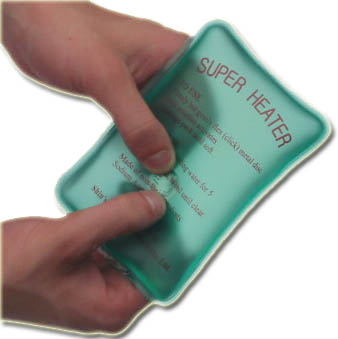
\includegraphics[width=.2\textwidth]{heatpack.jpg}
	\end{center}
	
	As a group, trigger one of the heat packs (you may know them as ``hand warmers'') on your table by clicking the button that's submerged in the liquid. Observe what happens within the heat pack during the first few minutes after triggering. Describe what you observe (i.e., tell each other a \emph{story} about what happened to the heat pack).
	
	In a few sentences, \emph{write on the whiteboard} your description (your story) of what you \textbf{\emph{observed}} (\textbf{\emph{not}} what you \emph{think} happened!). Please use words that everyone in your group is comfortable with. \textbf{Write clearly so that everybody in the room can read!}
	
	\bitem{Freezing liquid water}
	
	Based on your everyday experience, describe what you have to do to freeze water). After you have discussed this in your group for a few minutes, write your group's response on the board.
	
	\note{}{
		Desired kinds of responses something like ``put in a cold place'' or ``take heat out''
		Encourage groups to work together at board and not just have one student do all the work
	}
	
	\bitem {Does the behavior of a heat pack make sense?}
	
	Discuss in your group:
	\begin{enumerate}
		\item Based on your everyday experience with freezing things, would you say that the heat pack ``froze'' when it was triggered?
		\item Why or why not?
		\item Does the behavior of the heat pack make sense to you? Why or why not?
	\end{enumerate}
	Write your thoughts in response to (a), (b), and (c) on the whiteboard.
	\note{Possible responses}{
		\begin{enumerate}
			\item maybe/maybe not
			\item got hard and solid like ice, but didn't have to put it in a cold place. Got hotter than when a liquid.
			\item Does NOT make sense?
		\end{enumerate}
	}

\WCD

\end{benumerate}

\note{}{
	Use what students have on board to focus the summarization of the three prompts. Pick out groups to share what they have written on a particular prompt. Asking ``Why?'' and ``How do you know?'' are always good questions to ask as students present. Encourage students to speak loudly, so all can hear.
}

\subsection[Using models to make sense of physical phenomena]{Using models to make sense of physical phenomena: Introducing the \ThreePhaseModel{}}

\note{}{
	Ask students what they think of when they hear the word model. Accept all responses, but suggest confining to examples having to do with ``representing''. 

Ask students what they think a ``Scientific Model'' is.

Responses: 
Representation of certain ideas.


It is likely that any discussion of models in the first lecture didn't make much of an impression on students. Students need to get used to the idea that at one level, a model is simply the collection of ideas and relationships among those ideas, along with useful ways to represent the relationships that are needed to make sense of a particular class of phenomena, make explanations, predictions, etc. The model contains everything you need, including procedures built into the representation, that make your life much easier when doing both forefront science or responding to a quiz question.

One major goal of this first activity is to begin to get across these ideas about models. 

Intuition is good, helps us to make quick decisions and respond quickly (especially when the tiger is getting close!), but is not always so good at helping us on a quiz question. Using a model(s), on the other hand, gives you a lot of assurance that you will be on the right track (and get a good grade)

You might read the three paragraphs on the Activity Sheet to the students, have them read silently, and then summarize. However you do it, Please don't skip this part and some discussion of it.
}

\begin{reading}
\label{ReadingRefiningIntuitions}

	Before we can {\em make sense} of the process that occurs when the heat pack is triggered, we need to organize what we know about freezing and melting. You probably studied the processes of freezing and boiling in several previous science classes -- in a physical science class or chemistry in high school and perhaps in a college chemistry class. You have also had a good deal of everyday experience with freezing and boiling. But it is likely that your knowledge about these processes and phases of matter is somewhat fragmented and not well organized. Pulling together what we know and getting it organized in a useful way is what we need to do.

	\subsubsection*{{\em Learning Science} means {\em Refining Intuitions} and {\em Organizing Knowledge}}

	We all have everyday experience with lots of physical processes and phenomena. Sometimes, our intuitions seem to initially contradict the ``accepted scientific understanding.'' This is true for beginning scientists and experienced researchers alike! To continually improve our understanding of the world, we often need to refine our intuitions. In fact, we do this every day, while interacting with people, things, and situations in our environment. We use what we know about the world to make sense of our surroundings. Sometimes, we have to reorganize what we know in order to understand a new situation, and sometimes we learn something new altogether, new knowledge that we have to somehow fit in with what we already know. When this new knowledge organization becomes ``second nature'' to us, we have refined our intuition. 

	\subsubsection*{Models help scientists organize knowledge}

	One tool scientists use to organize knowledge related to a class of phenomena is the {\em scientific model}. Models bring together in one place the ideas and data patterns we use to make sense of phenomena in a concrete and useful way. A model represents these ideas in such a way that we can readily access them and use them. That is, a model typically provides the representational tools needed to use the model to develop explanations, make predictions, and more generally to make sense of phenomena. Over time, the features of a model will become second nature to us; we will have refined our intuitions about the phenomena in question.

\end{reading}

\subsubsection*{The \ThreePhaseModel{}}

	\note{}{	Probably should read this short paragraph to the class.}

	The \ThreePhaseModel{} provides a summary of the ideas needed to make sense of phase changes in matter (really, it only applies to so-called ``pure substances,'' but we won't make that distinction yet). There are instances, however, when the ``standard model'' is not sufficient to understand certain phenomena that undergo a phase change. This is the case with the heat pack. We have to extend the model, which is what we will do together in the following activities.
	

\begin{center}
\label{figTempVsEnAdd}
\begin{tikzpicture}[thick,scale=0.75, every node/.style={transform shape}]
	% title the diagram
	 \draw (7.5,7) node[align=center] {\textbf{\TempGraph{}}};

    % draw horizontal axis
    \draw[-{Stealth[scale=1.2]}, line width=1pt] (0,0) -- (14.5,0);
    % label the horizontal axis
    \draw (7.5,0) node[below=3pt] {Energy Added or Removed $\Delta E$ (at constant pressure)};

    % draw vertical axis
     \draw[-{Stealth[scale=1.2]}, line width=1pt] (0,0) -- (0,7);
    % label the vertical axis
     \draw (0,7.2) node[left=10pt, rotate=90] {Temperature $T$};
    % add melting point and boiling point on axis
     \draw[line width=1pt] (-3pt,1.8 cm) -- (3pt,1.8 cm) node[left=3pt] {\scriptsize{$T_\text{MP}$}};
     \draw[line width=1pt] (-3pt,3.8 cm) -- (3pt,3.8 cm) node[left=3pt] {\scriptsize{$T_\text{BP}$}};

	% draw first segment
	 \draw[line width=.8pt,dashed] (0,0) -- (1.5,1.8) node[below left=10pt, rotate=50.19442891] {\tiny{solid phase}};
	 
	% draw second segment
	 \draw[line width=.8pt,dashed] (1.5,1.8) -- (6,1.8) node[below left] {\tiny{mixed phase: solid/liquid}};
	 
	% draw third segment
	 \draw[line width=.8pt,dashed] (6,1.8) -- (8,3.8) node[below left=10pt, rotate=45] {\tiny{liquid phase}};

	% draw fourth segment
	 \draw[line width=.8pt,dashed] (8,3.8) -- (11.5,3.8) node[below left] {\tiny{mixed phase: liquid/gas}};

	% draw fifth segment
	 \draw[line width=.8pt,dashed] (11.5,3.8) -- (14,6.5) node[below left=10pt, rotate=47.20259816] {\tiny{gas phase}};
	 
	% draw labels
	 \draw[{Stealth[scale=.8]}-, line width=.4pt] (1.5,1.8) -- (1,2.8) node[above,align=center] {\tiny{All solid at $T_\text{MP}$}};
	 \draw[{Stealth[scale=.8]}-, line width=.4pt] (6,1.8) -- (5.5,2.8) node[above,align=center] {\tiny{All liquid at $T_\text{MP}$}};
	 \draw[{Stealth[scale=.8]}-, line width=.4pt] (8,3.8) -- (7.5,4.8) node[above,align=center] {\tiny{All liquid at $T_\text{BP}$}};
	 \draw[{Stealth[scale=.8]}-, line width=.4pt] (11.5,3.8) -- (11,4.8) node[above,align=center] {\tiny{All gas at $T_\text{BP}$}};
\end{tikzpicture}
\end{center}


%	\begin{center}
%		\label{figTempVsEnAdd}
%		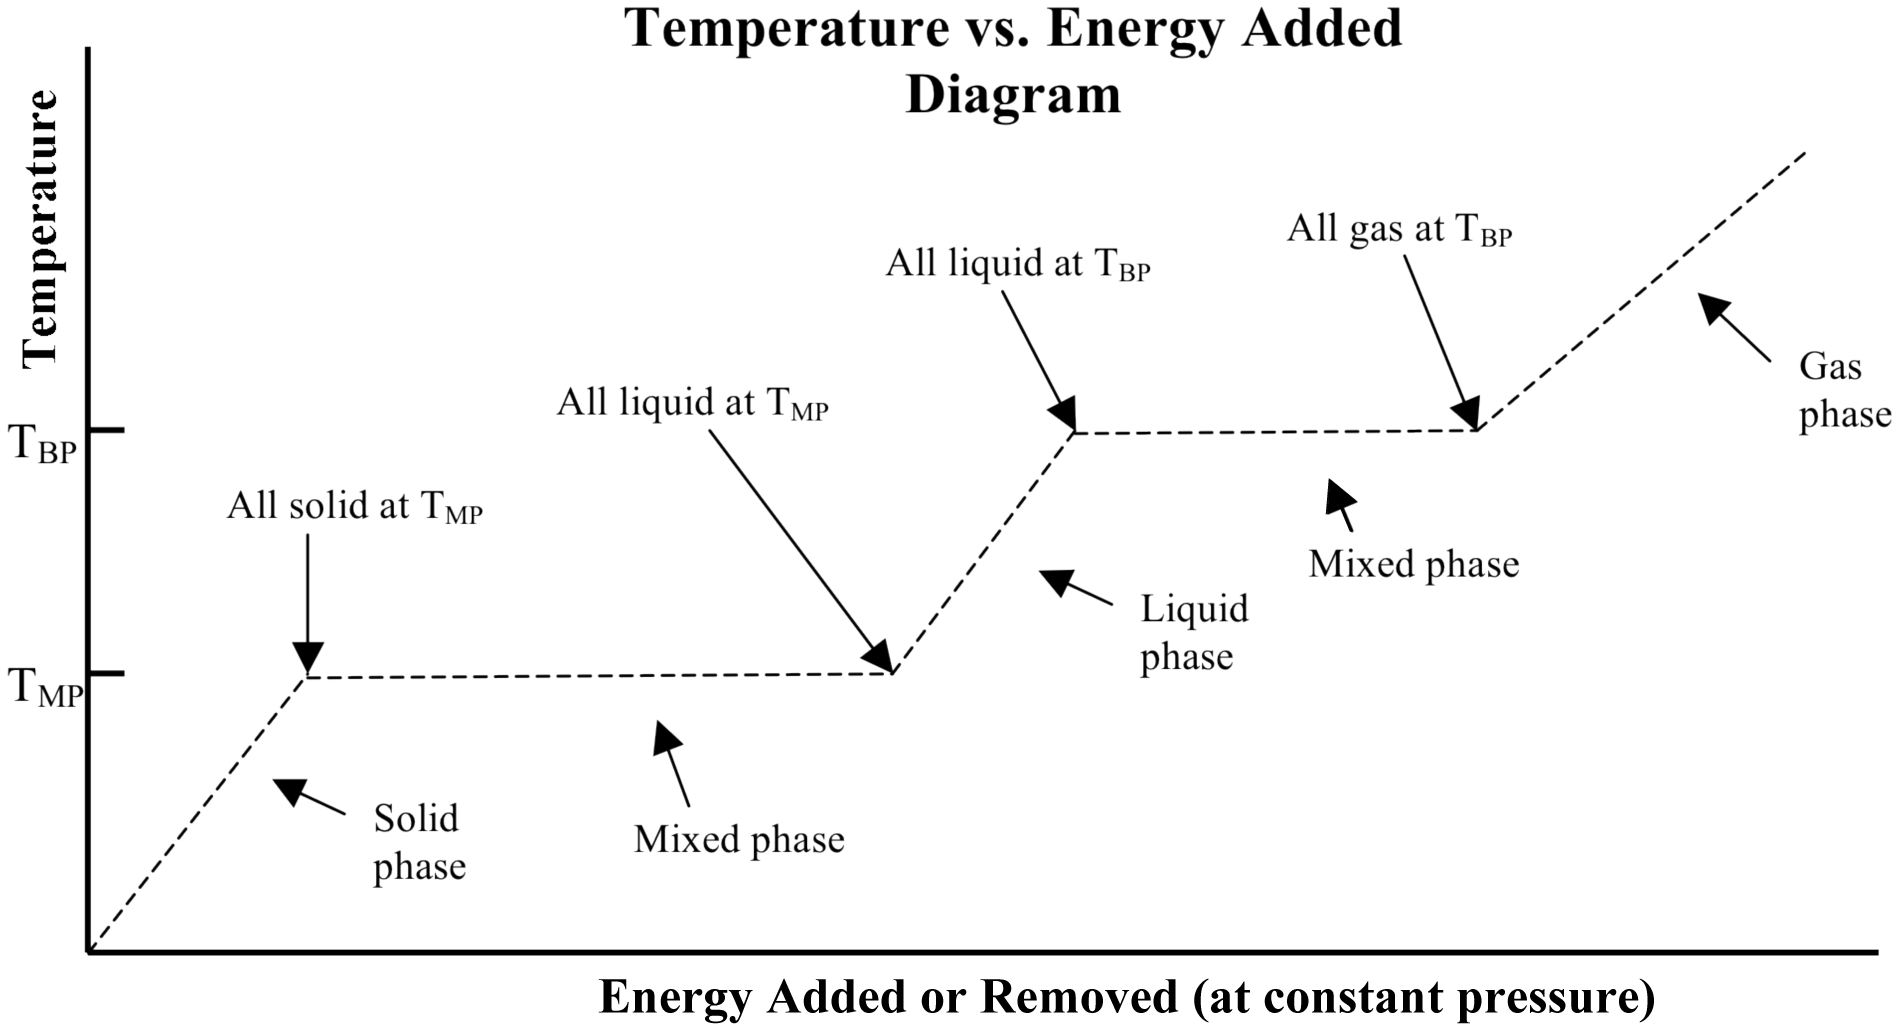
\includegraphics[width=.6\textwidth]{threephasemodel.png}
%	\end{center}

\begin{benumerate}
	\bitem {Examine the \ThreePhaseModel{} Summary}
		
	There should be several copies of the model summary sheet on your table. You can also find this summary in the online resources. Take about five minutes to look at what is on the summary sheet. Then focus on the diagrammatic representation: The \emph{\TempGraph{}}. Discuss with your group what the axes mean.
	
	\note{}{Make sure the groups have their Model Summary Sheets out and actually answer the question regarding the axes.}
	
	\bitem {Use the \ThreePhaseModel{} to construct a general explanation}

	\begin{enumerate}
		\item Put a sketch of the complete \TempGraph{} on your whiteboard that shows all three phases. Put a large dot on the graph that would represent tap water at room temperature.
		
		\item Now with the whole group participating, have someone put their finger on the dot and the rest of the group (take turns) describing what is happening to the water (tell another story!) as it is brought to a boil in the electric hotpot on your table. The person with their finger on the dot should move her/his finger along the graph to match the description. Imagine you leave the heating pot on for five or ten minutes, but not so long that all the water boils away. Now imagine putting the pot in your freezer for an hour or so and move your finger accordingly along the cooling curve.
		
		\item Repeat (b) over and over until everyone in your group is ready to explain to the whole class what goes on as you heat a substance way up and when you cool it way down. Use the language of the \ThreePhaseModel{} in your description, and use the diagram to illustrate your explanation.

\WCD

	\end{enumerate}
	\note{}{
		\begin{enumerate}
			\item Make sure every group gets their graphs on the board.  Also, make sure they get the ``dot'' in the right place.
			\item It is really important that all students in the group participate in these activities.
			\item Make sure all students are participating and that groups are taking this seriously.
		\end{enumerate}
	}

\note{}{
	Don't skip this.  ``Randomly'' call on few individual students to illustrate various processes. They need to be using phrases such as ``when you put energy (heat) in it melts more of the ice. This is represented on the graph by moving along the lower flat portion. The temperature stays constant while this happens, because the graph is horizontal here.''

	\subsubsection*{NOTE on NOMENCLATURE}
	Without making too much of a fuss about it, encourage students to use the word ``heat'' as a verb; e.g., ``We heat the water.''  ``Energy'' is what is put into or transferred to the water, during the process of heating it up.
}

	\bitem {Prepare the experiment}
	
	Use the model (and your knowledge of freezing and boiling points of water) to make a prediction (i.e., \textbf{don't start boiling the water yet!}) about temperatures:
	
	\note{}{Tell students to plug in their hot pots, but to unplug if the water starts boiling before they get to part (d).}
	
	\begin{enumerate}
		\item The hotpot in front of you should be filled about two thirds full with water. What temperature range does the model predict for the liquid water? I.e., what temperatures can liquid water have before it freezes or boils, according to the model?
		
		\item Suppose you begin heating the water. Immediately after the water has begun to boil, what does the model predict for the temperature of the liquid water? What about after it has boiled for five minutes? Compare your initial intuition with what the model tells you the temperature absolutely must be (assuming the model is appropriate for this phenomenon).
		
		\item If the lid is kept tightly on the pot and you have one thermometer immersed in the liquid and another one just above the surface of the liquid, and the water has been boiling vigorously for several minutes, what does the model tell you about the two temperatures?

	\end{enumerate}
		
	\bitem {Do the experiment}

	\begin{enumerate}
		\item Check out the model's predictions with the hot pot and the two thermometers you have at your table. On the board make a chart and compare your predictions from part 3 with your experimental results.
		
		\item Are there issues in the design of the experiment you just performed that are not taken into account in the model?  Describe these on the board and be prepared to discuss them with the class.

	\end{enumerate}

\textbf{Remember:} Make sure your responses are legible, and that your entire group agrees with what is written on the board.

	\note{}{
		\begin{enumerate}
			\item Because it is in the liquid phase, the Model for water says it must be between 0 and 100$^\circ$C.
			\item 100$^\circ$C both immediately and five min later, since we assume it will not have boiled away yet.  Make sure they get why and how the model says this.  Our intuition often tells us that the temperature will rise above 100$^\circ$C as we continue to heat it, but if the water is in the mixed phase, it must be at 100$^\circ$C according to the model.
			\item The straight-line part of the graph tells us that the temperature will be the same as long as there is some liquid and some vapor, since we are in the mixed phase.  (We assume there is nothing but water vapor -- no air -- in the space above the water.)
			\item Tell students to plug back in.  Make sure lids are on tight to prevent air getting into the pot.  Vapor should be coming out $v_i$gorously where the thermometer goes in.  When this is the case, the vapor temp is close to 100$^\circ$C.
			\item The model assumes the vapor and the liquid are in thermal equilibrium.  This implies that there is negligible energy leaving the vapor inside the top of the pot and going to the atmosphere.
			\item You will probably need to hurry the students along.
		\end{enumerate}
	}

\WCD

\note{}{
	Resolve any discrepancies among group's responses. You can ask students to compare their response with other group's responses and point out any differences.  Come to a class consensus on any discrepancies.

	Part (e) begins to get at a subtle point that we will keep coming back to.  We can be sure of our ``answers'' in terms of what the model says.  This is the level we expect the students to achieve: understand the models sufficiently well to use them to construct explanations and make predictions with high certainty that they know what they are doing.  The harder part is knowing how well the model actually fits the experimental situation/phenomenon and not making unwarranted assumptions about what can be left out of a model or what must be put in.  For (e), the model makes a completely certain prediction that the temperature in the vapor and liquid is the same, because in the model, the assumption is that the two phases are in equilibrium.  This assumption may or may not be reasonable in a real world phenomenon.  Of course, we could develop a much more sophisticated model to more precisely predict the temperature of the vapor in the top of the hot pot, but that is not our aim here. 
}

	\bitem {What does the model say?}
	\label{Part B 3j}
	
	Use the \ThreePhaseModel{} to answer the following question:
	
	When two phases of a substance are present and in thermal equilibrium (i.e., both phases have the same temperature), what do you know with certainty about certain properties or physical conditions as they relate to that substance?

	\note{}{
		The following is NOT an intuitive notion.  But it is an important aspect of the behavior of substances as they go through phase changes.  It is also Very Apparent from the graph --- the straight line --- IF the students stop to think about what the graph means.  Many students NEVER think through what the graph means!  This is a BIG part of what we want them to learn to do.
	}
	
	Discuss in your group. How does the model representation help you answer this question?

\WCD

\end{benumerate}

\note{}{See above.}
	\newpage
	\section[Analyzing a Heat Pack]{Analyzing a Heat Pack Using the \ThreePhaseModel{}}
\label{act1.1.2}

\todo[inline]{I noticed that many times, the "\ThreePhaseModel{}..." is referred to as "\ThreePhaseModel{}" without hyphen. This is a minor issue, but we should be consistent. I've replaced it in this file, but maybe we can automatically find/replace this in all files while importing?

-BH}
\todo[inline]{I've got a python script that will take care of this. It's in the \texttt{python} folder and called \texttt{ctrl\_r.py}. You're welcome to edit the list of stuff to search for and change at the beginning of the script or leave me a note and I can do it.

-EH}

\note{Timing: \unit[40]{min}}{
	
	\subsubsection*{Purpose}
		\begin{itemize}
			\item Provide practice using the \ThreePhaseModel{} applying it to the heat pack.
			\item Provide awareness that a general model, in this case the \ThreePhaseModel{}, might not apply without modification in some situations such as cooling of sodium acetate (heat pack) through the freezing temperature.
		\end{itemize}
	
	\subsubsection*{Learning Outcomes}
		\begin{itemize}
			\item Be able to explain how a specific scientific model can be used to constrain what aspects of a phenomenon need to be taken into account and what it means to make sense of a phenomenon in terms of a model.
			\item Be able to explain during which heating and cooling processes of a heat pack can be explained using the simple \ThreePhaseModel{} and which processes cannot.
		\end{itemize}
}

\begin{overview}
	\noindent
	{\bfseries Overview:} Our goal is to make sense of the heat pack behavior using both the \ThreePhaseModel{} and the \EnergyInteractionModel{}. We'll start with a focus on the \ThreePhaseModel{}.

\end{overview}

\subsection{Macroscopic properties and energy transfers}
\label{A1}

When analyzing a physical phenomenon, a model greatly simplifies and restricts what we focus on. \textbf{The constructs that make up the model {\em limit} the aspects of the phenomenon that we must pay attention to.}

\begin{enumerate}
	\item Using {\em only} the constructs of the {\bfseries \ThreePhaseModel{}}, what are \textbf{\em macroscopic properties} of the heat pack that changed (and how did they change) during the first few minutes after triggering?
	
		Look at the Model Summary Sheet and try to use only those words.
		
		Write your new story on the board.
		
	\note{Optimal student response}{
		``{\em Temperature} increased and {\em phase} changed from liquid to solid.''
		
		Students should be focused on macroscopic properties of the model, not simply repeating their response to the first question in \hyperref[act1.1.1]{Act.~\ref*{act1.1.1}}; e.g., color changed from clear to white.
	}
	\note{General}{
		Make sure all SGs actually write these things on the board. You will probably have to encourage them to do so. A loud announcement directed to the whole class can be effective with this kind of reminder. Make sure the students get used to following these instructions to write responses on the board.
	}

	
	\item How does the amount of energy associated with clicking the small disk inside the heat pack compare to the other energy transfers that occur? Think, for example, about the amount of heat transferred from the heat pack to your hands or to the environment.
	 
	 	Is it about the same amount of energy? Much larger? Much smaller?
	 	
	 	Write your group's response on the board.
	
	\note{}{
		Help students convince themselves that the mechanical energy associated with the trigger is insignificant compared with the other energy changes and transfers. You can suggest they repeatedly squeeze a liquid heat pack other than on the disk and see if it makes it any warmer.
	}

\WCD

\end{enumerate}

\note{}{
	\begin{itemize}
		\item Pick out one or two groups to share their responses to each of the questions. Alternatively, you can read responses from one or two groups. You can ask the whole class if they like the way a particular response is worded or how it could be improved, etc. Try to get them to do the explaining!
		\item Students should leave this discussion with the notion that a lot more energy ``comes out'' as heat than was put in with the clicker. You can talk about the clicker action as simply a ``trigger.''  So, the bottom line, which you should state, is that we agree that changes in clicker energy-systems are not significant and that a lot of energy comes out as heat.
	\end{itemize}
}

\subsection{Completing the cycle}

\note{General}{
	Suggest to the class that they can start this part before the Whole Class Discussion has occurred for the previous part. Remind them to put their response on the board and to constantly refer to the \textbf{\ThreePhaseModel{}} Summary and to use that language.
	
	{\em Don't wait for all groups to finish before wrapping it up in the Whole Class Discussion.}
}

Now, let's take the heat pack we had triggered before through the rest of its cycle.

\begin{enumerate}
	\item Read and follow the instructions on the heat pack to get it back to being a liquid at room temperature.
	\item Describe qualitatively and briefly how the properties of the heat pack identified in part \ref{A1} changed during the rest of the cycle. Write your new story on the board.
\end{enumerate} 

\noindent\textbf{Attention:} You will continue your analysis of the heat pack in your homework assignment. Therefore, please write down in your notes how the properties changed as the heat pack went through its complete cycle. You will need this!

\WCD

\note{}{
	DL instructor should quickly summarize the changes in temperature and phase of the pack when it is in the boiling water and then cools down to room temperature. Students should understand that this takes the pack through a cycle, i.e.\ it returns to the original state. You can remind them that one of their homework assignments will ask them to diagram a series of processes that take the heat pack through an entire cycle.
}

\subsection{Using our model}

\begin{enumerate}
	\item Think about your response to \hyperref[Part B 3j]{question~\ref*{Part B 3j}} in \hyperref[act1.1.1]{Activity~\ref*{act1.1.1}}.\footnote{Here's the question again, for reference, and so you don't need to flip back and forth: ``When two phases of a substance are present and in thermal equilibrium (i.e., both phases have the same temperature), what do you know with certainty about certain properties or physical conditions as they relate to that substance?''} When your heat pack is in a mixed solid/liquid state, what do you know about its temperature?
	
		Use this knowledge to experimentally determine the melting-point temperature of the heat pack. In order to ensure equilibrium conditions, you can minimize energy transfers to or from the heat pack by wrapping plastic bubble-wrap around the heat pack and thermometer. You can also fold your heat pack around the end of the thermometer.
		
		Does it matter how you attained the mixed state: melting when in the hot pot or freezing when triggered?
		
		Record your result on the board, indicating a ``direction'' on your diagram.
	
	\note{}{
		In principle, the phase temp between solid and liquid can be determined by getting to the phase change going from either direction. It is much easier, however, to get an equilibrium mixed state going from liquid to solid by triggering, rather than using a hot water bath to partially melt a solid heat pack. Don't let the SGs spend any significant amount of time figuring out that triggering is the quickest way to achieve the equilibrium phase change temperature. The main point is you want both phases in equilibrium. (T$_\text{MP} \approx 54^\circ$C)
	}
	
	\item Two processes that you can readily observe with the heat pack are: i) changing from liquid to solid and ii) changing from solid to liquid.
	\begin{enumerate}
		\item For which of these two processes does the heat pack seem to follow the predictions of the {\bfseries \ThreePhaseModel{}} and for which process does it \textbf{\em not} follow the model? Be brief, but specific. Put your response on the board. [Hint: Use your finger to trace the graph.]
		
		\item For which of these two processes does the heat pack behavior pretty much agree with your intuition about phase changes? For which process does it not agree? Put your response on the board. Does your intuition now agree pretty much with the model? If not, what is different?
	\end{enumerate}
	
	\note{}{
		The liquid to solid phase transition does not occur as predicted by the model. As the heat pack is cooled it remains in the liquid state significantly below the phase change temperature. Melting a solid heat pack in boiling water does follow the model. 
	}
	
\WCD

\end{enumerate}

\note{}{
	DL instructor does brief summary of entire activity. Main points are:
	\begin{itemize}
		\item Liquid/solid phase change temperature is $\sim54^\circ$C.
		\item The heat pack follows the \ThreePhaseModel{} when going from solid to liquid, but not going from liquid to solid.
		\item The heat pack drops below the temp at which it should change to a solid, instead remaining a liquid. We give the label (name) supercooling to this phenomenon of staying a liquid below the phase change temp. (Don't go into any more detail. There is a homework exercise on how to represent this on a Temp to Energy Added Diagram, with follow-up discussion in the \hyperref[act1.1.5]{Activity~\ref*{act1.1.5}}. This will be the first example of modifying and extending a model.
	\end{itemize}
}	
	\newpage
	\section[\ThreePhaseModel{} \& \EnergyInteractionModel{}]{Practicing the \ThreePhaseModel{}; Introducing the \EnergyInteractionModel{}}
\label{act1.1.3}

\note{Timing: \unit[40]{min}}{

	\subsubsection*{Purpose}
		\begin{itemize}
			\item Provide practice applying both the \ThreePhaseModel{} and the \EnergyInteractionModel{} to various phenomena.
		\end{itemize}

	\subsubsection*{Learning Outcomes}
		\begin{itemize}
			\item Capable of drawing \EnergyDiagrams{} for simple physical processes
		\end{itemize}
}

\begin{overview}
	\noindent
	{\bfseries Overview:} We briefly interrupt our efforts of making sense of the heat pack to get a bit of practice using the \ThreePhaseModel{} and to introduce the \EnergyDiagram{}.
\end{overview}

\note{}{``All members of your group must now go to the board and work on the following together.'' You must enforce this. Students need to interact with each other and not let one or two students do all the work.  Having them all at the board really helps here.}

\noindent\textbf{Your instructor will assign one or more of the following physical processes to your small group:}

\begin{enumerate}[(a)]
	\item Cooling a piece of solid copper (Cu) from \unit[500]{\textdegree C} to \unit[350]{\textdegree C}.
	\item Warming a piece of ice from \unit[-20]{\textdegree C} to the melting point.
    	\item Condensing steam completely to liquid at \unit[100]{\textdegree C}.
	\item Completely sublimating a chunk of dry ice at \unit[-79]{\textdegree C}.
	\item Partially melting 25\% of ice initially at \unit[0]{\textdegree C}.
	\item Heating a piece of copper initially at \unit[300]{\textdegree C} until it is half melted.
	\item Cooling and completely freezing \ce{H2O} initially at \unit[80]{\textdegree C}.
\end{enumerate}

\noindent {\bfseries For each of these processes, sketch the following on your whiteboard and be prepared to explain to the whole class:}

\begin{enumerate}[(i)]
	\item A complete \TempGraph{} (remember, this is the graphical part of the \ThreePhaseModel{}) with the initial and final states clearly marked; 
	
	{\bfseries and }
	
	\item An {\em open} \EnergyDiagram{}. Refer to ``Steps Involved in Using the \EnergyDiagram'' on the \EnergyInteractionModel{} summary on your table. Try your hand at translating your \EnergyDiagram{} into an algebraic expression of energy conservation.
\end{enumerate}

	
\begin{center}
%	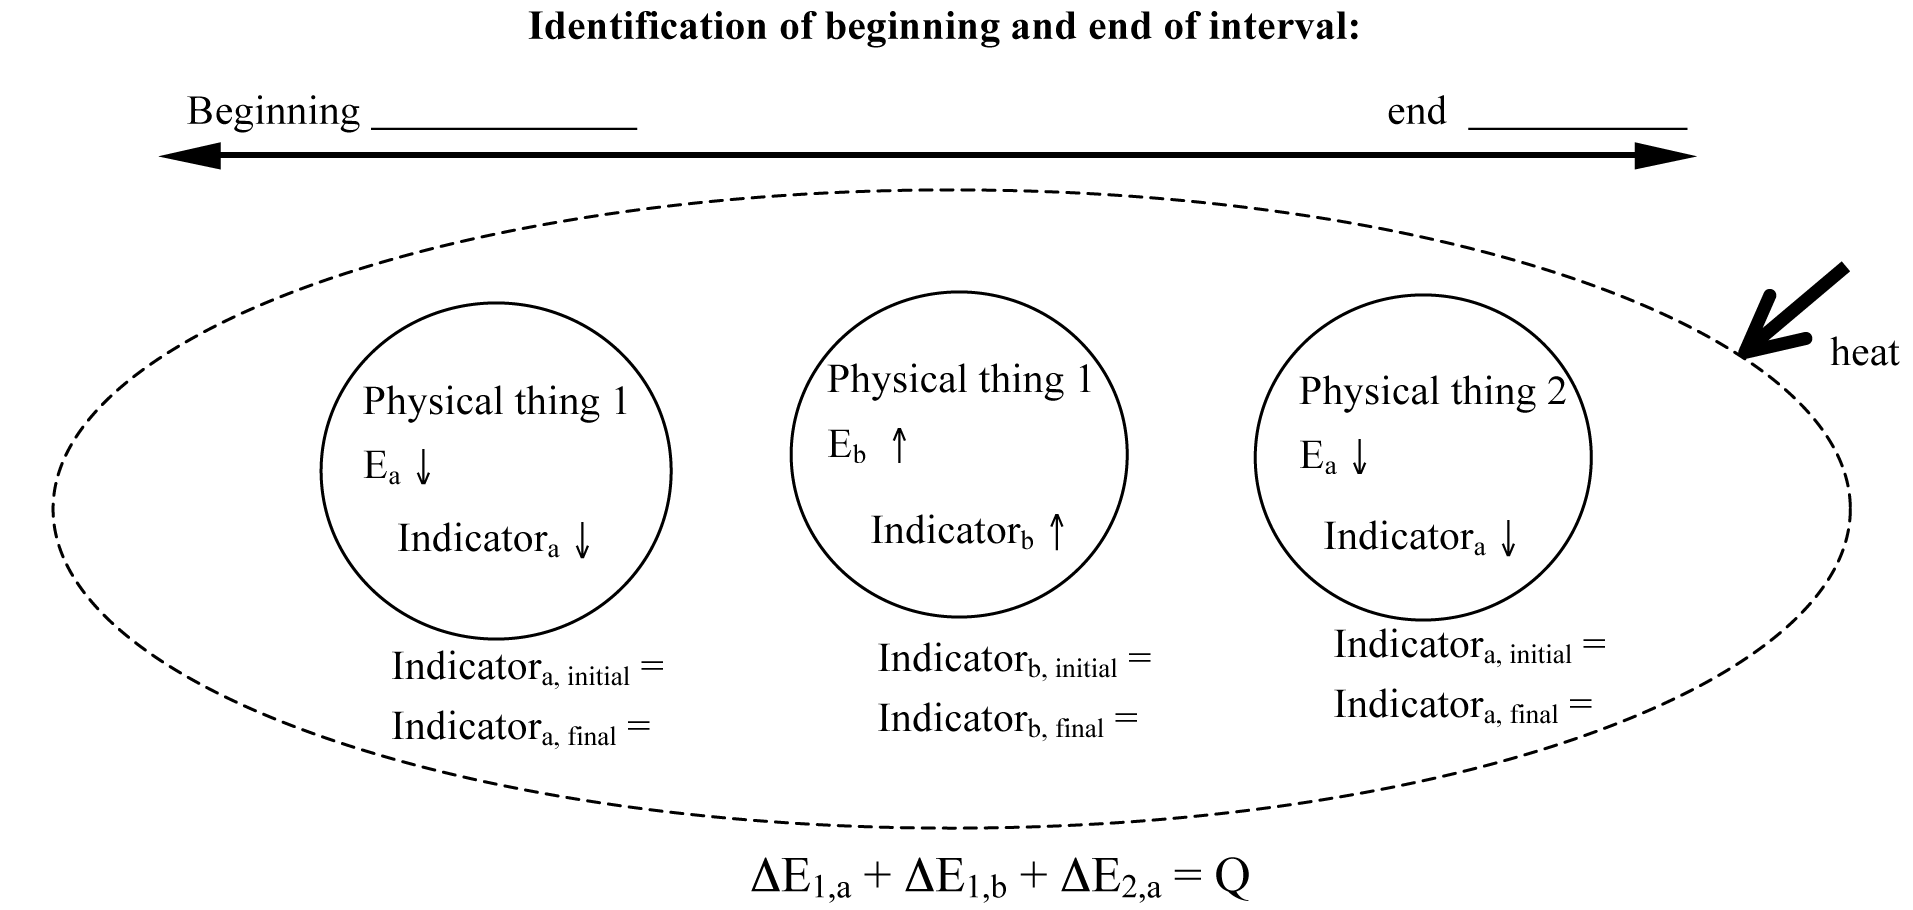
\includegraphics[width=0.7\linewidth]{E-ID}
	
\begin{tikzpicture}[thick,scale=0.75, every node/.style={transform shape}]
    % draw horizontal line   
    \draw[-{Stealth[scale=1.2]}, line width=1pt] (0,0) -- (10.2,0);

    % draw vertical lines
    \foreach \x in {0.5,9.5}
      \draw[line width=1pt] (\x cm,3pt) -- (\x cm,-3pt);

    % title the diagram
    \draw (5,0) node[above=18pt] {\scriptsize{\textbf{Identification of \emph{beginning} and \emph{end} of interval:}}};

    % draw nodes along the interval timeline
    \draw (0.5,0) node[below=3pt] {\scriptsize{initial conditions}} node[above=3pt] {\emph{beginning}};
    \draw (9.5,0) node[below=3pt] {\scriptsize{final conditions}} node[above=3pt] {\emph{end}};

    % draw the physical system boundary
    \draw [dashed,orange,line width=1pt] (5,-2.75) ellipse (6cm and 2.25cm) node[above=1.5cm] {\textbf{\emph{physical system}}};
    
    % draw energy systems
    \draw (2,-3) node[draw,circle,blue,minimum size=2.25cm,inner sep=0pt,align=center]  {\color{darkgray}\tiny{indicator $a$}\\[.5ex]$\downarrow E_\text{1,a}$\\\color{darkgray}\tiny{$a_i =$}\\[-1.2ex]\color{darkgray}\tiny{$a_f =$}} node[orange,above=1.1cm] {\scriptsize{physical thing 1}};
    \draw (5,-3.25) node[draw,circle,blue,minimum size=2.25cm,inner sep=0pt,align=center]  {\color{darkgray}\tiny{indicator $b$}\\[.5ex]$\uparrow E_\text{1,b}$\\\color{darkgray}\tiny{$b_i =$}\\[-1.2ex]\color{darkgray}\tiny{$a_f =$}} node[orange,above=1.1cm] {\scriptsize{physical thing 1}};
    \draw (8,-3) node[draw,circle,blue,minimum size=2.25cm,inner sep=0pt,align=center]  {\color{darkgray}\tiny{indicator $a$}\\[.5ex]$\downarrow E_\text{2,a}$\\\color{darkgray}\tiny{$a_i =$}\\[-1.2ex]\color{darkgray}\tiny{$a_f =$}} node[orange,above=1.1cm] {\scriptsize{physical thing 2}};    

    % draw heat arrow
    \draw[{Stealth[scale=1.2]}-, line width=1pt, blue] (10,-2.25) -- (11,-1.5)  node[right=0cm] {heat Q};
    
    % write energy conservation equation
    \draw (5,-6) node[] {$\Delta E_\text{1,a} + \Delta E_\text{1,b} + \Delta E_\text{2,a} = Q$};
    \draw (3,-6) node[above=6pt] {\scriptsize{$(-)$}};
    \draw (4.6,-6) node[above=6pt] {\scriptsize{$(+)$}};
    \draw (6.15,-6) node[above=6pt] {\scriptsize{$(-)$}};
    \draw (7.35,-6) node[above=6pt] {\scriptsize{$(+)$}};

\end{tikzpicture}
\end{center}

\note{Procedure}{
	\begin{itemize}
		\item Assign one process to each SG.  If a SG finishes early, have them do another.  You could also have them tell you how to draw one on the board.
		\item Tell students to study the example of an \EnergyDiagram{} on two-page blue model summary.
		\item Remind the students that all of these are very straightforward, and should be mastered quickly.  Any complicated process will require the coordination of multiple energy systems. These should be thought of as ``exercises.''
	\end{itemize}
	
	You do not necessarily have to get through all of these by the end of DL, but if you can at least cover the first three they should be able to finish the remainder. They are also assigned as part of the FNTs.
	
	Some of the processes are not stipulated sufficiently to guarantee a unique diagram (e.g., Process~3). That's ok. They can discuss/compare the different possibilities.
}


\noindent \textbf{Again, \emph{you need to be prepared} to explain and describe the process you have been assigned to the whole class using both models.} When you use the \ThreePhaseModel{} trace the process with your finger as you describe it. Make sure you clearly show the beginning and ending points of the process in the diagram.\\

\textbf{NOTE:} You will have an opportunity to rework these examples in the \hyperref[fnt1.1.3-1]{homework}. These are all very straightforward once you're familiar with the basic ideas of the two models. Working through these examples will also give you practice in applying the models and using the representations with a variety of phenomena. It is very important that you can do this quickly and correctly (i.e., it should become \emph{second nature} to you). When applying these models to make sense of more complicated phenomena, e.g., on a quiz, it is crucial that you are not stumbling over the basics.

%\todo[inline]{This WCD seems squished to the Note above it. I have no idea why this happens and how to fix it. It'd be good if this could be formatted consistently throughout the book. Maybe using an environment?}
\WCD

\note{}{
	Have each group explain how their \TempGraph{} matches their \EnergyDiagram{}.
	
	{\em You should have already corrected any gross errors as they are putting them up.}
	
	After a group has presented, you should ask the whole class if there is anything that is left out or that should be worded in a better way, etc.  This is an opportunity to help all students see what properly drawn diagrams should be like.
	
	{\em You should have groups correct any mistakes or omissions on their diagram on the board. This helps provide closure for everyone.}
}

\note{}{
	Shown below are examples of \EnergyDiagrams{} for Processes 1 and 3.  Notice that the indicator for bond energy systems is treated differently in the diagram than indicators for other energy systems, i.e., they are not required to record specific initial and final values of mass.
	
	\begin{multicols}{2}
		Process 1\\		
		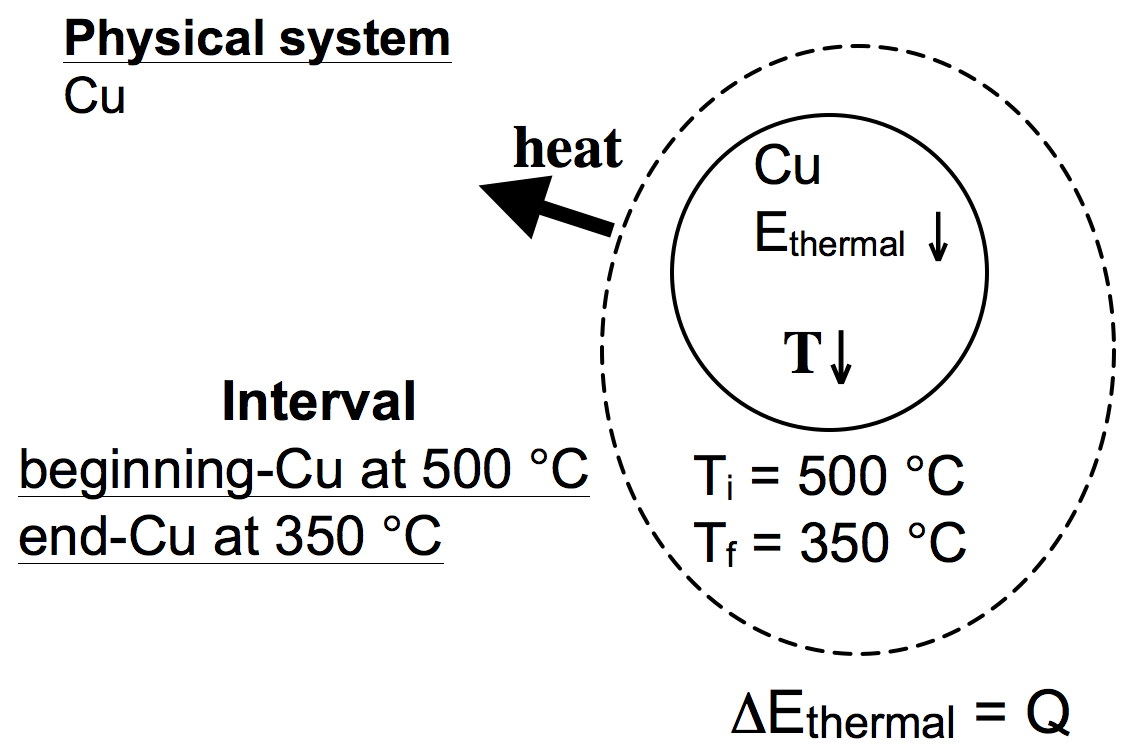
\includegraphics[width=0.9\linewidth]{act113-1}
		
		\columnbreak
		Process 3\\		
		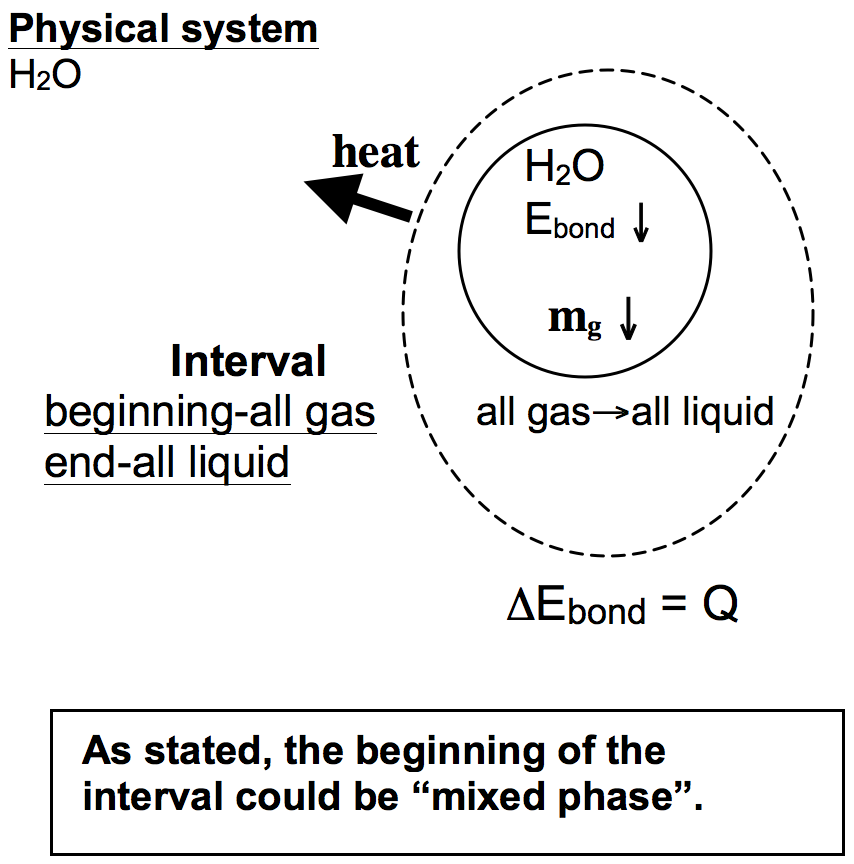
\includegraphics[width=0.9\linewidth]{act113-3}
	\end{multicols}
}


%%%%%%%%%%%%%%%%%%%%%%%%%%%%%%%%%%%%%%%%%%%%%%%%%%%%%%%%%%%%%%%%%%%%%%%%
%
%		DLM 3
%
%%%%%%%%%%%%%%%%%%%%%%%%%%%%%%%%%%%%%%%%%%%%%%%%%%%%%%%%%%%%%%%%%%%%%%%%

\chapter[\chaptername\thechapter]{\chapterlongname \thechapter}
\label{dlm3}
\addchapter

%	\iftoggle{instructor}{\note{}{\input{U1/dlm3-overview}}\newpage}{}
	\note{Brief Overview}{
	The first two CLASP Activities in this DLM continue \hyperref[dlm2]{DLM\ref*{dlm2}} with the qualitative study of both the \ThreePhaseModel{} and the \EnergyInteractionModel{}. They extend the work you did on the FNTs assigned at the end of \hyperref[dlm2]{DLM\ref*{dlm2}}.
	
	The last CLASP Activity begins \texttt{Module 1.2}: Getting Quantitative with Models.
	
	\subsubsection*{If you run out of time to complete DL Activities}
	
		In general, for any unfinished DL activities from the previous DL (which should have been assigned as an FNT), give a brief summary (\textless \unit[5]{min}) at the beginning of the current DL and sum up the main points for them. Don't spend time in DL as you normally would having the students discuss and explain.
	
	\subsubsection*{Instructor notes}
	
		Read the instructor notes before the TA meeting!! They contain not only answers (to most of the questions), but also information about what the students should be getting out of the activity, and, at times, instructions on how to run the activity. Be prepared to ask questions in the DL meeting to clarify anything you are not sure of, e.g., ``What is important for the students to get from this?''
		
	\subsubsection*{FNTs}
	
		This is the first time the students will see what they are expected to do with the FNTs. Specifically, they all should have worked hard on them outside of class. Then, in their small groups, they will have the opportunity to clear up their uncertainties about making \EnergyDiagrams{} and using them to make sense of physical phenomena. You should ``check off'' the FNTs or in some way note which of your students have put in an acceptable amount of effort working on them and which have not. Students need to know that you are keeping a record of whether they are doing their homework or not. What's important is that they work on the FNTs, not that they ``get them exactly right'' when they first do them.
		
	\subsubsection*{Explanations on the board}
	
		Students are often asked to write explanations in words on the board. Encourage them to outline, abbreviate, paraphrase, use sentence fragments, etc. in order to reduce the time required to write those explanations. In other words they don't have to be quite as careful in producing explanations for WC consumption as they should on exams, because they can easily clarify in the WC discussion.
	
	\subsubsection*{No equipment needed for DLM03}
}

\note{Reminder}{The goal in this course is ``making sense,'' not getting answers.}

\section{Practicing Our Two Models}
\label{act1.1.4}

\begin{overview}

	\noindent
	{\bfseries Overview:} We continue to practice using the \ThreePhaseModel{}, and we'll start to get more familiar with the \EnergyDiagrams{} of the \EnergyInteractionModel{}.

\end{overview}


\note{Timing: \unit[65]{min}}{

	\subsubsection*{Purpose}
		\begin{itemize}
			\item To become more familiar with the \ThreePhaseModel{} and the \EnergyInteractionModel{}, the meaning of the model constructs and the diagrammatic representations of the models
			\item To become more familiar with applying these two models to particular thermal processes
		\end{itemize}
	
	\subsubsection*{Learning Outcome}
		\begin{itemize}
			\item Be able to quickly and confidently apply both the \ThreePhaseModel{} and the \EnergyInteractionModel{} to the kinds of phenomena treated in this activity. This means being able to confidently use the diagrammatic representations of both models to develop explanations and answer specific questions related to these kinds of thermal phenomena.
		\end{itemize}
}

\subsection{Basics of the \ThreePhaseModel{}}

\begin{fnt}
	\label{fnt1.1.1-1}
\subsubsection*{Scientists don't come up with ``right answers.''}

Usually, when your instructor asks you to ``do problems'' for homework or on a test, they expect you to get a ``right answer,'' right? Well, we don't. As a matter of fact, for many of the problems you will encounter in this course, there won't be one ``right answer.'' Science just doesn't work that way. For every problem, there are a number of ways one can approach the problem, and each different solution path might result in different answers. But, that doesn't mean that one of them is ``right'' and the others are not.

\subsubsection*{Scientists come up with arguments.}

Much more important than an answer to a question or problem in science is usually the method by which one arrived at this answer. So, our emphasis is on the method you use to solve a problem. The pathway to your solution. \textbf{We want to know what assumptions and decisions you're making as you solve a problem, and how you're using these assumptions and decisions to \emph{make an argument} for \emph{your} solution.} That's how science works! There is nobody who knows ``the right answer.'' But there are people who can look at what you've done and who can tell you whether the assumptions you've made are appropriate in a particular situation and the argument you've constructed is valid and convincing. In science, this is called ``peer-review'' because the people who look at your work are other scientists.

\subsubsection*{So, if we don't care so much about you ``getting the right answer,'' how will we evaluate your progress in this course?}

Just like in a scientific publication, \textbf{we ask you to be \emph{very specific} about what you did and did not do, and \emph{how} you arrived at a particular solution to a problem.} We'll practice this a lot, so that you know what we expect from you. This first problem is an extreme example of what problem-solving in this class looks like for you: \emph{We'll actually give you some answers.} A little further down, you'll find a box with some answers that one might reasonably get when solving this problem. Note that we're not saying these are the exact answers you will get or that we expect you to get! But your solutions to this problem might be quite similar to the ones given below.

\subsubsection*{Now, if we give you the answers, what do we want you to do?}

We want you to describe in detail how you are using the diagram below to respond to the prompts in the problem. Write a story about the diagram and about how you are reading the graph to get the values you get. While this is stated a few times below, it's worth repeating: \emph{We don't want you to do any calculations for this problem!} Instead, use the diagram and tell us \emph{how} you're using the diagram and \emph{why} we should believe you that your answer to the problem is a reasonable one.

Yes, this might be a bit more work than what you're used to from other classes. Later in this course, we'll find shorter ways for you to show us your work and argument. But for now, \textbf{\emph{please do write out a detailed story -- including your assumptions, decisions, etc. -- for each part of the problem.}}

\subsubsection*{On to the actual problem:}

Use the particular \TempGraph{} of the \ThreePhaseModel{} shown below to respond to the prompts in this FNT.\\

\noindent
{\centering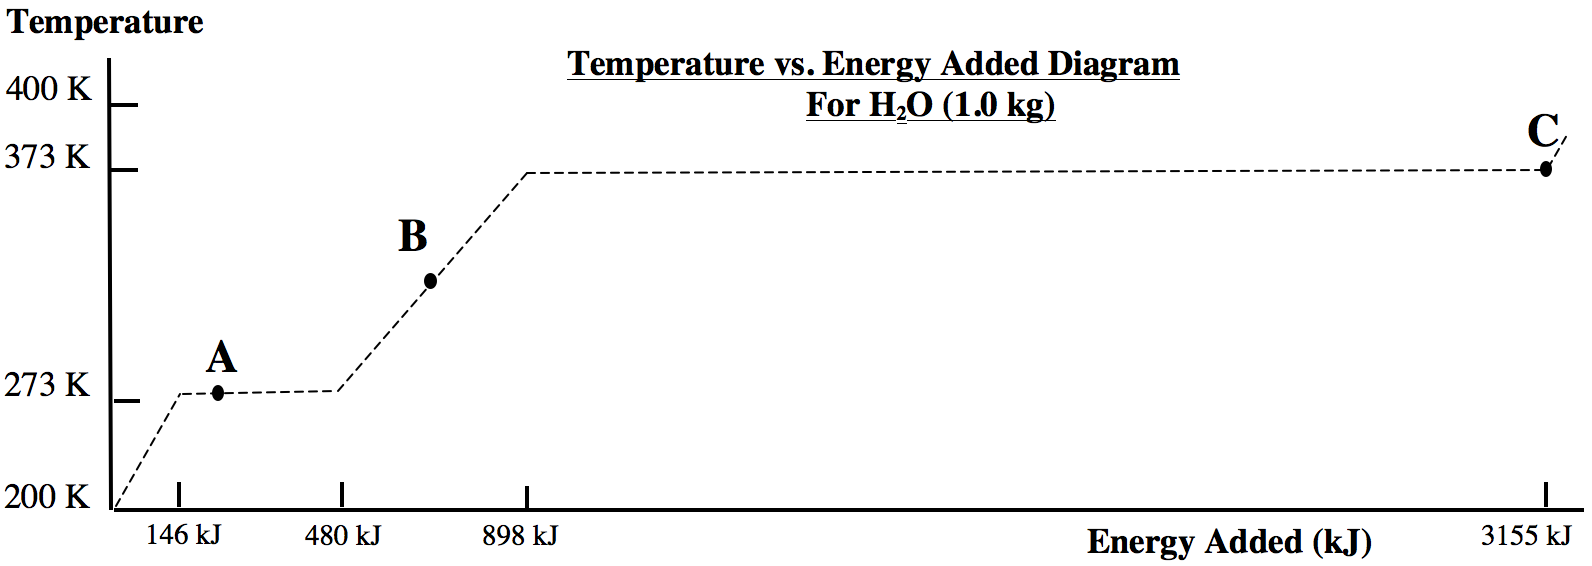
\includegraphics[width=.95\linewidth]{fnt111-1.png}\par}

\noindent The values along the $x$-axis (\unit[146]{kJ}, \unit[480]{kJ}, etc.) are the amounts of energy that must be added to get the \unit[1.0]{kg} of water from an initial temperature of \unit[200]{K} to the next phase change. For example, \unit[480]{kJ} is the total amount of energy that must be added to the water starting at the initial temperature of \unit[200]{K} to completely melt all the ice.

\begin{enumerate}
	\item Describe what is happening at each of the ``corners'' on the graph. What phase is the water in at the letter A, B, C?
	\label{fnt1.1.1-1A}
	
	\item Assume that you have one kilogram of water at an initial temperature of \unit[200]{K}. If \unit[795]{kJ} of energy is added, describe the final state (approximate temperature and phase) of the water. If the water is in a mixed phase, determine very approximately the percent in each phase.
	
		You are not expected to do any calculations at this time. Simply tell us what the diagram tells you (and how you know that it does).
	\label{fnt1.1.1-1B}
	
	\item Repeat \hyperref[fnt1.1.1-1B]{Part~\ref*{fnt1.1.1-1B}} but with \unit[146]{kJ} of energy added to the water initially at \unit[200]{K}.
	
	\item Repeat \hyperref[fnt1.1.1-1B]{Part~\ref*{fnt1.1.1-1B}} but with \unit[1650]{kJ} of energy added to the water initially at \unit[200]{K}.
	
	\item State the initial and final conditions of the process that takes the system from Point C to Point B and determine very approximately how much energy would have to be added or removed.
	\label{fnt1.1.1-1C}
	
	\item Repeat \hyperref[fnt1.1.1-1C]{Part~\ref*{fnt1.1.1-1C}} for water initially in State A and ending in State C.
	\label{fnt1.1.1-1D}
	
\end{enumerate}

\subsubsection*{Again: Do not make any calculations to respond to these prompts!}
\end{fnt}
\note{}{
	Get students started checking their responses to this FNT as they come into the room.
	
	Before the WC discussion, ask each group to put the response to one of the prompts in \#2 of the Activity on the board. Then in the WC discussion, ``randomly'' call on someone from each group to explain how they knew how to respond to that prompt. Emphasize that they really need to know how to use this modeling tool: the \TempGraph{}.
	
	You might also call on someone to explain anything in part \#1 if you feel it is necessary.
}

\noindent
You've all done this FNT individually at home. Now you have an opportunity to practice creating scientific arguments together. Back up your claims with evidence and try to convince each other of \emph{your} solution!

\begin{enumerate}
	\item Discuss with your group and make sure \emph{every} group member is confident that she/he can explain \hyperref[fnt1.1.1-1A]{Question~\ref*{fnt1.1.1-1A}} on the FNT.
	
	\item While there is not one single correct answer for \hyperref[fnt1.1.1-1B]{Parts~\ref*{fnt1.1.1-1B}} -- \hyperref[fnt1.1.1-1D]{\ref*{fnt1.1.1-1D}} of the FNT, you probably estimated the values somewhere in the vicinity of those in the box. Work out in your small groups any significant discrepancies you might have. EVERYONE in your group should be ready to explain how you obtained these results in the whole class discussion. Your instructor will tell your group which prompt you should respond to on the board.
\end{enumerate}

\begin{ans}
	\begin{enumerate}\setcounter{enumi}{1}
		\item liquid at \unit[$\sim$350]{K}
		\item completely solid at \unit[273]{K}
		\item $\sim$1/3 gas, $\sim$2/3 liquid at \unit[373]{K}
		\item initial conditions: all gas at \unit[373]{K}, final conditions: liquid at \unit[$\sim$50]{\textdegree C}; $\Delta$E~$\approx$~\unit[2470]{kJ}
		\item initial conditions: $\sim$25\% liquid at \unit[0]{\textdegree C}, final conditions: gas at \unit[100]{\textdegree C}; $\Delta$E~$\approx$~\unit[3000]{kJ}
	\end{enumerate}
\end{ans}


\WCD

\subsection{Basics of the \EnergyInteractionModel{}}

%\noindent
%{\bfseries Overview:} Using the \EnergyInteractionModel{} to describe simple processes.

\begin{fnt}
	\label{fnt1.1.3-1}

Neatly write out all of the \EnergyDiagrams{}, with the accompanying \TempGraphs{}, listed below (these are the same scenarios that were requested in \hyperref[act1.1.3]{Activity~\ref*{act1.1.3}}).

Remember that complete \EnergyDiagrams{} always include algebraic expressions of energy conservation. Refer to the \EnergyInteractionModel{} discussion in the online resources.

\begin{enumerate}[(a)]
	\item Cooling a piece of solid copper (Cu) from \unit[500]{\textdegree C} to \unit[350]{\textdegree C}.
	\item Warming a piece of ice from \unit[-20]{\textdegree C} to the melting point.
	\item Condensing steam completely to liquid at \unit[100]{\textdegree C}.
	\item Completely sublimating a chunk of dry ice at \unit[-79]{\textdegree C}.
	\item Partially melting 25\% of ice initially at \unit[0]{\textdegree C}.
	\item Heating a piece of copper initially at \unit[300]{\textdegree C} until it is half melted.
	\item Cooling and completely freezing H$_2$O initially at \unit[80]{\textdegree C}.
\end{enumerate}


\end{fnt}
\note{}{
	{\em Stress} to the WC that they should have little trouble with these. They need to look at ``General Process of Constructing an \EnergyDiagram{}'' and quickly compare with each other. Give no more than \unit[5]{min} to do their comparing.
	
	You can ask if there are any issues the entire SG is unsure of, and then respond to the WC very briefly.
}

\begin{enumerate}
	\item Compare your responses for the processes in \hyperref[act1.1.3]{Activity~\ref*{act1.1.3}}, both the \TempGraphs{} and the \EnergyDiagrams{}.
	
	\item Your instructor will tell you which one of the scenarios (a) through (g) to put on the board.
		
	Put the \TempGraph{} and the \EnergyDiagram{} near each other. Make sure the two diagrams are consistent with each other and make sure everyone in the group can explain precisely why both are drawn the way you have them.

\WCD

\end{enumerate}

	\newpage
	\section[The Heat Pack and New Thermal Phenomena]{Making Sense of the Heat Pack: Exploring New Physical Phenomena}
\label{act1.1.5}

\begin{overview}

\noindent
{\bfseries Overview:} We return to our efforts of making sense of the heat pack by using both the \ThreePhaseModel{} and the \EnergyInteractionModel{}. In the process, we'll explore some new, related thermal phenomena -- \emph{Super-Heating} and \emph{Super-Cooling} -- and we'll see that we have to modify the standard \ThreePhaseModel{} to describe and understand the heat pack.
	
\end{overview}


\note{Timing: \unit[\about50]{min}}{
	
	\subsubsection*{Purpose}
		\begin{itemize}
			\item To provide more practice making sense of a ``strange phenomena,'' the heat pack, by applying the standard \ThreePhaseModel{} to some parts the heating and cooling cycles of a heat pack
			\item Seeing how to extend/modify the \ThreePhaseModel{} to include super-cooling
			\item Seeing how this extension of the \ThreePhaseModel{} is an example of how models start out as simple as possible and are then made more sophisticated as new data-patterns are incorporated
		\end{itemize}
	
	\subsubsection*{Learning Outcome}
		\begin{itemize}
			\item Be able to use the \ThreePhaseModel{} and the \EnergyInteractionModel{} to explain the behavior of a sodium acetate heat pack during each heating and cooling process of its entire cycle.
		\end{itemize}
}

\note{}{
	The \textbf{THEME} of this activity is to use the {\em representations of the two models}, i.e., the \EnergyDiagram{} and the \TempGraph{}, in an analytic way, rather than having ``to know the answer'' or asking the instructor The models are more than just the collection of relationships (equations); a model like these contains explicitly in the representations the procedural knowledge needed to figure out what to do next when ``you don't know what to do.'' 
}


\subsection{Taking the Heat Pack through its Entire Cycle}

\begin{fnt}
	\label{fnt1.1.3-2}

When using the \EnergyInteractionModel{} to make sense of the behavior of a heat pack (or really, any thermal cycle), it helps to divide the overall process (cycle) into multiple sub-processes.  Use the following sub-processes:

\begin{center}
\begin{tabular}{llll}
	\hline\hline
	&	Initial conditions	&	Action	&	Final Conditions\\
	\hline
	(a)	&	liquid at \unit[100]{\textdegree C}	&	taken out of boiler	&	liquid at \unit[23]{\textdegree C}\\
	(b)	&	liquid at \unit[23]{\textdegree C}	&	triggered	&	solid/liquid at \unit[54]{\textdegree C}\\&& (and insulated)	& shortly after triggering\\&&& (in mixed state)\\
	(c)	&	solid/liquid at \unit[54]{\textdegree C}	&	sitting on table	&	 solid at \unit[23]{\textdegree C}\\
	(d)	&	solid at \unit[23]{\textdegree C}	&	placed in boiler	&	solid/liquid at \unit[54]{\textdegree C}\\
	(e)	&	solid/liquid at \unit[54]{\textdegree C}	&	left in boiler	&	liquid at \unit[100]{\textdegree C}\\
	\hline\hline
\end{tabular}
\end{center}

\noindent Make four \EnergyDiagrams{}, one for each sub-process (a), (c), (d), and (e), but NOT (b). Also, make a \TempGraph{} for each process. Make sure you can describe each process {\em in your own words} using both of the representations. 
\end{fnt}

%\subsection*{\em All members of your group must now go to the board and work on the following together.}

\note{}{
	This really does work best if the whole group is up at the board. This is one of the most effective ways to encourage discussion between the members of the small groups. Keep encouraging students to just stand at the board at all times instead of going back and forth between sitting in chairs and standing at the board...
}

\note{General directions}{
	\begin{itemize}
		\item Assign one part of this FNT to each group to put on the board \textbf{BUT NOT part (b) yet!} These parts: (a), (c), (d), and (e) are pretty straightforward. Make sure the students are clearly specifying the interval, getting the indicators correct, and writing the algebraic equation for energy conservation as
		\item $\Delta E_\text{system} = Q$  and the open \EnergyDiagram{} shows Heat (the word, not the symbol ``$Q$'') with an arrow pointing in or out as appropriate.  The symbol ``$Q$'' is a signed variable, so it can be confusing for the better students, who recognize this to have arrow pointing in either direction
	\end{itemize}
}

	\noindent{\bfseries Very important for the following}: Make sure everyone in your group is ready to {\em explain} to the whole class \textbf{\em how} they know the answers to the following questions (detailed instructions below):

\begin{enumerate}

	\item Does each energy system increase or decrease?
	\item Is this an open or closed system with respect to energy, and if open, does energy come in or leave?
	\item How are your responses consistent with your \TempGraph{}?
	\item And finally, how do both diagrams tell you about the sign of each term in the equation expressing energy conservation?
	
\end{enumerate}

	\noindent To make this task a bit more manageable, your instructor will assign one of the four heat pack processes listed in \ref{fnt1.1.3-2} to your group:  (a), (c), (d), or (e) -- note that we're not concerned with part (b) yet. For your assigned process, put on the board both 
	\begin{enumerate}[(i)]
		\item an \EnergyDiagram{},
		
	{\bfseries and}
		
		\item a \TempGraph{}.
	\end{enumerate}
	
	\noindent{\bfseries Make sure that} the two representations of the process are in agreement and that everyone in your group can explain why they are drawn the way they are. Refer to ``Steps Involved in Using the \EnergyDiagram'' on the model summary page. 

\WCD

\note{}{
	\begin{itemize}
		\item To keep this short, they don't need to explain how they constructed the entire diagram, but give the WC the opportunity to ask them about any questions they have.
		
		\item Definitely have each SG explain how they know whether each energy system in their diagram increases or decreases, and what that tells them about the sign of each term in their algebraic expression of energy conservation.
		
		[\textbf{Why is this important?} Many students fail to realize that the \EnergyDiagram{} can give knowledge ({\em with absolute certainty}) of the algebraic sign of each $\Delta E$ term.  This needs to be stressed repeatedly to the students because the great majority of them have (largely unconsciously) adopted the strategy: ``find and plug into an equation!'']
		
		\item Also stress that the \TempGraphs{} MUST agree with the \EnergyDiagram{} if there is any energy in or out.
	\end{itemize}
}

\subsection[The Clicking Mystery]{The Clicking Mystery: Super-heating and super-cooling}

\noindent
As we'll find out here, we have to modify the standard \ThreePhaseModel{} to illustrate what happens in the heat pack. Let's start with some preparations in this FNT.

\begin{fnt}
	\label{fnt1.1.3-3}

We want to analyze triggering step (b) in \hyperref[fnt1.1.3-2]{\thefnt} more closely using the \TempGraph{} of the \ThreePhaseModel{}. This will help us get a deeper understanding of this part of the process and will enable us to extend the \ThreePhaseModel{} to make it more realistically explain actual phenomena. (It turns out that super cooling and super-heating are rather common. Usually, however, they occur over a very small temperature range and so go unnoticed.)

\begin{enumerate}
	\item Sketch a \TempGraph{} for sodium acetate between room temperature at approximately \unit[150]{\textdegree C}, assuming the sodium acetate does not undergo any super-cooling, i.e., assuming that the heat pack is solid at room temperature, and changes phase at its normal phase change temperature, which you determined in \hyperref[act1.1.2]{Activity~\ref*{act1.1.2}}.
	
	\item On the same diagram, sketch the path representing the process of the liquid heat pack cooling down from \unit[150]{\textdegree C} to room temperature with no phase change (now assuming there is supercooling). Check that the path you sketched makes sense by verifying that the changes in temperature and energy shown on the diagram as you move along the path you sketched match what you know about the actual changes in temperature and energy of the heat pack as it cools to room temperature without changing phase from liquid to solid.
\end{enumerate}
\end{fnt}

\note{General directions}{
	Try to get most of their mistakes cleared up {\em before} the Whole Class Discussion. As they put up diagrams that have mistakes, instead of just telling them what is wrong, have them ``interpret'' what they have diagrammed by having them {\em start at the initial state} on the diagram and tell you what their diagram is describing {\em as the process proceeds}. Then ask them if that description matches the process in the FNT. [The lead instructor should explain this strategy]
	
	Make sure every group ends up with the correct combined graphs on their board, since they will need this for the next part.  The cooling curve is one diagonal straight line.  The heating curve is identical from 54 to \unit[100]{\textdegree C} and on top of the first curve, but at \unit[54]{\textdegree C} it has a horizontal section, which displaces the lower diagonal part to the left.
}

\begin{benumerate}

	\bitem{Extending the \TempGraph{}}
	
	Now you are going to take the two curves from \ref{fnt1.1.3-3}, and draw them ``on top of each other.'' The trick is to figure out where they exactly overlap and where the two curves deviate from each other.
	
	Erase your board and draw the \TempGraph{} fairly large that you drew for process 2 in \ref{fnt1.1.3-3}: Cooling from \unit[100]{\textdegree C} to \unit[23]{\textdegree C} with no phase change.
	
	Now, we are going to draw the combined heating process (d) plus (e) in the same diagram. \textbf{BUT WAIT!} The heating curve you draw will need to be ``on top of one another'' \textbf{where they describe the exact same state: namely warming or cooling the {\em liquid from \unit[54]{\textdegree C} to \unit[100]{\textdegree C}.}}
	
	They are in the same phase, liquid, when they are at \unit[100]{\textdegree C} (and consequently in the same state), but they are in different phases when they are at \unit[23]{\textdegree C}, so they are not in the same state. When they are in different states, the curves won't be on top of each other.
	
	Make sure your heating curve and cooling curve overlap where they are supposed to. Make sure everyone in your group knows {\em why} the two curves overlap the way they do.

\WCD

	\bitem {What happens when the clicker is clicked?}
	
	Now, to make the analysis a little simpler, let's assume this: When you activate your heat pack, it is thermally insulated -- like it is when wrapped tightly with bubble wrap.
	
	\textbf{Sketch the path} of the clicking process on the cooling curve you just made above -- starting at the bottom end of the cooling curve at \unit[23]{\textdegree C}. You can determine this new path after the click from what you know from your experiments about the temperature change, and from the implications of {\em heat-in} or {\em heat-out} because it was insulated with the bubble wrap.
	
	What state (temperature and phase) is the sodium acetate in {\em shortly after} the clicking has occurred and while still insulated? Use both what you know from your direct observation of the phenomenon and from your diagrams to draw this portion of the process (from \unit[23]{\textdegree C} to \unit[54]{\textdegree C}). Make sure the new part of the path you draw on the diagram (from before to shortly after clicking) describes this process.
	
	\note{Correct diagram}{
		The final part of the process in the \TempGraph{} will be a vertical line from the final state (liquid @ \unit[23]{\textdegree C}) to the horizontal part of the diagram (signifying a temperature change with no energy added or removed).
	}

\WCD
\note{}{
	It is important to conduct a wrap-up that is reassuring to the students without erring on the side of ``we will just wait until the instructor gives us the answers.''  Everything should have already been explained by now, so you are not telling them the answers.  But you are clarifying and extending the discussion, particularly on the supercooling part.  The supercooling part is a good example of how models get extended (and made more complicated).  Supercooling is actually a very common phenomenon, but usually it is not very noticeable.  Also, superheating is noticeable when bringing water to a boil in a clean container in a microwave oven.  The sudden boiling, when triggered by movement of the container, can be quite $v_i$gorous and dangerous.  You should emphasize these points in the wrap-up.
}

	\bitem {The \EnergyDiagram{} for clicking}
	
	Now make an \EnergyDiagram{} for the clicking process. Open or closed? Which energy systems? Which energy system increased and which decreased?
	
	What feature of your \EnergyDiagram{} tells you that the part of the graph in the \TempGraph{} that represents the ``clicking'' is simply a vertical straight line?
	
	\note{}{
		\noindent
		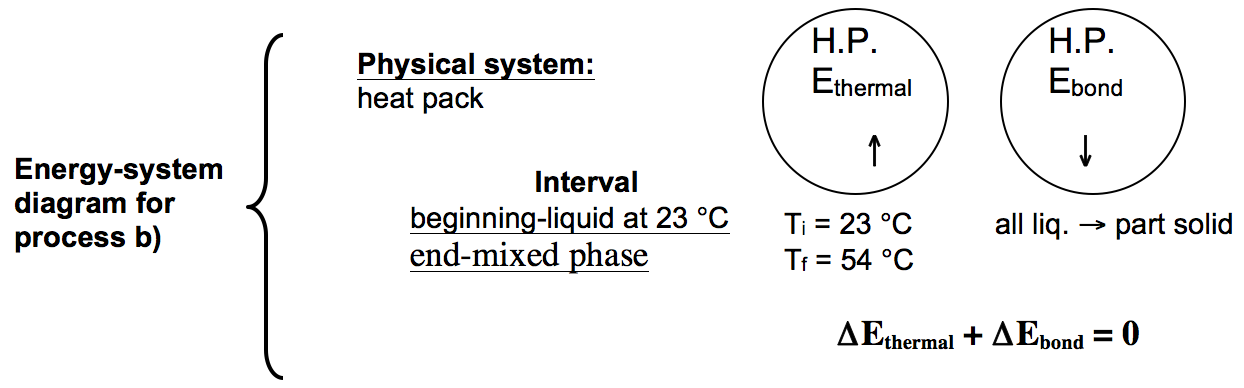
\includegraphics[width=\linewidth]{act115-chi}
	}

\WCD
\note{Pose the Question}{
	So where did the energy come from when the clicker is clicked?
	
	And: How do you know?
	
	Have the class answer this, making sure they can explain and how they know where it came from.
	
	Ans: Observe the partial phase change (bonds getting made) and $T$ going up; clicker adds insignificant energy
}

	\bitem {Getting back to room temperature}
	
	If you now partially remove the bubble wrap so the heat pack can exchange energy with the environment, sketch the rest of the path that gets the heat pack back to a solid at room temperature. Should this path fall ``on top of'' the heating path?
	
	\note{}{
		The \ThreePhaseModel{} assumes that in a mixed state, the two phases are in thermal equilibrium. After the heat pack is triggered it the temperature quickly increases to close to the melting point during initial solidification, but because the complete solidification process doesn't happen quickly (it involves hydration) the heat pack is typically far from being in thermal equilibrium as it cools from the melting temperature to room temperature. But, if we imagine it is still fairly well insulated, then the model prediction that it follows the standard horizontal line at the melting temperature until it is completely solidified would describe how a heat pack behaves. So, to the extent that the model applies to the heat pack phenomena of getting from a mixed state at the melting temp back to room temperature, it does so as the model predicts.  
	}
	
	\bitem {\ThreePhaseModel{} with Super-Cooling}
	
	Discuss in your small group how you can summarize the difference in the \ThreePhaseModel{} as applied to situations when there is and when there isn't significant/noticeable supercooling. Put your summary on your board and be ready to explain to the whole class.
	
	\note{}{
		Without supercooling the heating curve and cooling curve are identical.  When there is supercooling, the cooling curve in the liquid region will extend below the melting/freezing temperature. This means the substance can exist in the liquid state even when the temperature is below the freezing temperature. As the temperature is lowered further in the supercooled state, or when the substance is disturbed, it ``jumps'' vertically to the mixed state without absorbing or giving off heat to the environment.  (Note: supercooling also occurs when vapor cools below the boiling/condensation temperature and superheating occurs when a substance in the liquid phase is heated above the boiling point.
	}

\WCD

\end{benumerate}

\note{}{
	Let one or two groups take a stab at explaining the difference in the models with and without supercooling.  Perhaps the best summary is simply to compare the difference in the cooling curves and explain that the heating curves are the same. 
}

	\newpage
	\section{Getting Quantitative: New Thermal Properties}
\label{act1.2.1}

\begin{overview}

\noindent
{\bfseries Overview:} So far, we've used qualitative descriptions and we've estimated numbers to describe the thermal phenomena occurring in the heat pack. However, we often need to be able to accurately quantify our observations and come up with mathematical models that can hopefully give us precise predictions for measurements. In this section, we'll familiarize ourselves with some mathematical models for thermal properties. In particular, we'll talk about \emph{Heat Capacity and Specific Heat,} as well as \emph{Heat of Vaporization} and \emph{Heat of Melting}.

\end{overview}

\note{Timing: \unit[$\sim$30]{min}}{

	\subsubsection*{Purpose}
		\begin{itemize}
			\item To provide an opportunity to become familiar and comfortable using the constructs heat capacity, molar heat capacity, specific heat, and heats of vaporization and melting and how these constructs relate to the previously used constructs in the \ThreePhaseModel{} and \EnergyInteractionModel{}
		\end{itemize}
		
		This activity takes the qualitative analysis the students know how to do and makes it quantitative by incorporating the actual specific heats and heats of melting, etc.\ for specific substances. It also clarifies the difference between the intensive quantities of specific heats and the extensive quantity heat capacity. Similarly for $\Delta H$. The units used with $\Delta H$ (intensive quantity) or with lower case c (specific heat), clarify how to convert the intensive quantity to the extensive quantity that is usually of interest. Note: We consciously use notation that these particular students are most likely to come across in their chemistry and biology texts.
	
	\subsubsection*{Learning Outcomes}
		\begin{itemize}
			\item Understand and be able to describe/explain the constructs of heat capacity, heat, and a change in temperature.
			\item Understand and be able to describe/explain the connection between heat capacity and thermal energy.
			\item Understand and be able to describe/explain the difference between heat capacity, molar heat capacity, and specific heat and know how to decide when to use which one.
			\item Understand and be able to describe/explain how $\left|\Delta H_\text{VAP}\right|$ and $\left|\Delta H_\text{MELT}\right|$ connect to $\Delta E_\text{BOND}$.
		\end{itemize}
}


\noindent Your instructor will give you one or two minutes to discuss each of the following in the following parts~\hyperref[1.2.1A]{\ref*{1.2.1A}} and \ref{1.2.1B} in your Small Groups. Quickly come to a consensus and put your response on the board. Each question will be followed by a brief \framebox[1.1\width][c]{\textbf{Whole Class Discussion}}.

\subsection{Heat Capacity}
\label{1.2.1A}

\begin{enumerate}
	\item You may have used the relationship \framebox{$Q = C\Delta T$} in chemistry and physical science classes. \textbf{What does ``heat capacity'' mean \emph{in your own words?}} You don't have to put this on the board, but make sure everyone in your group is ready to explain.
		
	\note{}{
		Try to get answers that are not simply a restatement of an equation. ``Heat capacity,'' as all concepts, has a deeper meaning than an expression in a certain set of units. For example, an appropriate answer here might be: ``Heat capacity is a measure of the amount of heat that must be added to an object to raise its temperature; the greater the heat capacity, the more heat that must be added to raise an object's temperature a certain amount.''  
	}
		
	\item Imagine you have a big bucket of water and a small (like, European-sized) teacup of water, which would have the greater heat capacity -- the water in the bucket or in the teacup? Which would have the greater specific heat?
		
	\note{}{
		Bucket has much larger heat capacity, due to much larger quantity of water. Since both substances are the same, they have the same specific heat. This is an example of the difference between extensive and intensive quantities.
	}
		
	\item Create an \emph{open-system \EnergyDiagram{}} that illustrates the process of making a heat capacity measurement for the big bucket of water (adding heat to this water).\\
	\textbf{Note:} We are assuming that this measurement takes place at a \emph{constant volume} (no water is lost during the measurement). The significance of this will make more sense later in the course.
	\label{1.2.1A3}
		
	\note{}{
		\noindent
		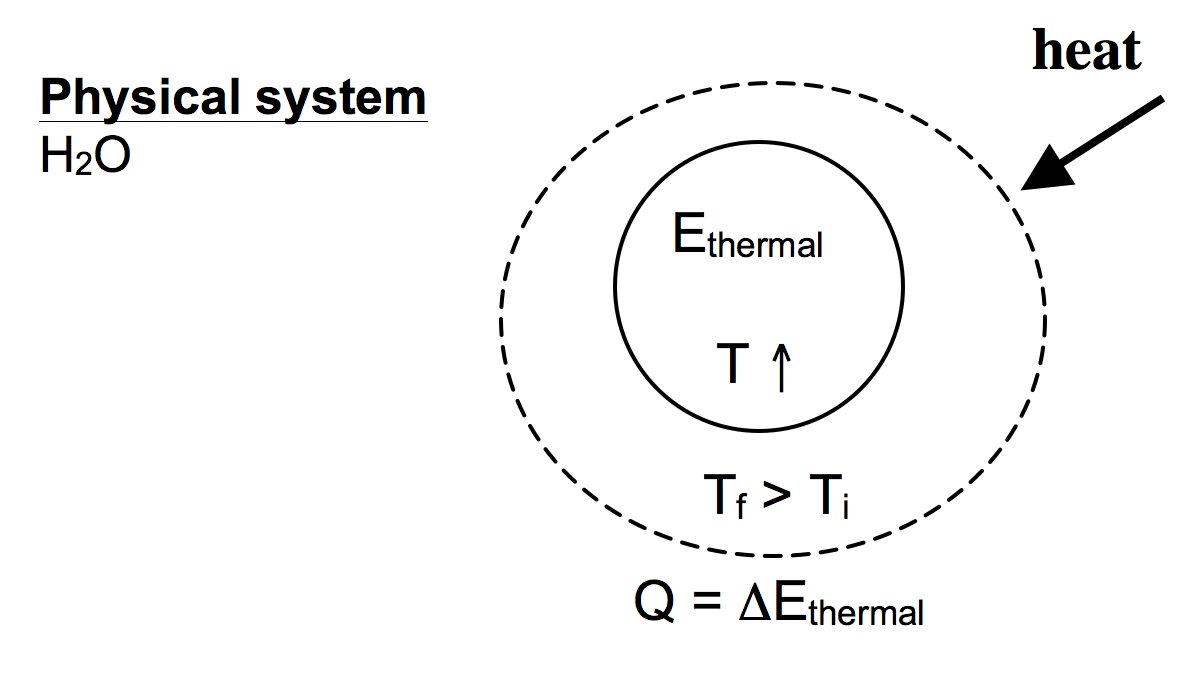
\includegraphics[width=\linewidth]{act121-3}
	}
		
	\item Use your diagram from (3) and the definition of heat capacity to develop an algebraic relationship that relates change in thermal energy to temperature change and heat capacity.
		
	\note{}{
		$\Delta E_\text{thermal} = C \Delta T$
		
		[$C$ units are \unitfrac[]{J}{K}    units for $\Delta T$ can be in either Celsius orr $KE$lvin, since the size of the degree is the same]
	}
		
	\item Use the following definitions to determine simple algebraic relationships between the heat capacity and each of two specific heats (mass \& molar): 
	
	\begin{itemize}
		\item Mass specific heat is the heat capacity per kilogram,
		
		\textbf{and}
		
		\item Molar specific heat is the heat capacity per mole.
	\end{itemize}	

	In what situations would one or the other be more useful or convenient to use?
		
	\note{}{
		Mass specific heat, $c_m = \nicefrac{C}{m}$; $m$ is mass.
		
		Molar specific heat, $c_n = \nicefrac{C}{n}$; $n$ is \# of moles.
	}
\end{enumerate}

\subsection{Heat of Vaporization and Heat of Melting}
\label{1.2.1B}

\begin{enumerate}
	\item You may have used the relationship \framebox{$Q = \Delta H$} in chemistry and physical science classes. \textbf{What does ``heat of melting'' -- or ``heat of vaporization'' -- mean \emph{in your own words?}} As above, you don't have to put this on the board, but you should make sure everyone in your group is ready to explain.
	\label{1.2.1B1}
	
	\note{}{
		They should say something like, ``Heat of vaporization'' is a measure of the amount of heat that must be added to a substance to totally vaporize it.
	}
	
	\item Use the \EnergyInteractionModel{} to illustrate a process in which $Q = \Delta E_\text{BOND}$.
	
	\note{}{Same as \hyperref[1.2.1A3]{\S\ref*{1.2.1A}\#3}, with bond energy instead of thermal energy.}
	
	\item If $\left|\Delta H\right|$ were given in units of joules per kilogram (\unitfrac[]{J}{kg}) or units of joules per mole (\unitfrac[]{J}{mol}), instead of units of joules, how would the equation, $Q = \Delta H$, change?
	\label{1.2.1B3}
	
	\note{}{
		$Q = \pm \left|\Delta H\Delta m\right|$, where $\Delta m$ means the amount of mass that changed phase; similarly for units of joules/mole, with $\Delta n$ instead of $\Delta m$. 
		
		This gets at the distinction between intensive and extensive quantities. To change an intensive quantity to an extensive quantity, such as $\Delta H$ as it is used in \hyperref[1.2.1B1]{\S\ref*{1.2.1B}\#1} (where it has units of joules), you have to multiply by the amount of the substance in the units the intensive quantity is expressed in. The two expressions in \hyperref[1.2.1B3]{\S\ref*{1.2.1B}\#3} are the most common intensive expressions for $\Delta H$. When $\Delta H$ is used as an intensive quantity, it would typically have a subscript, such as $\Delta H_\text{vap}$, but this is not a hard and fast rule and $\Delta H$ as an extensive quantity could also be subscripted. You and your students need to always be aware of the specific context.
	}
	
	\item Use questions 1 through 3 above to describe a specific relationship between the change in bond energy in our \EnergyInteractionModel{}, and the indicator of the bond energy system (i.e., the portion of mass of a substance that changed phase).
	
	\note{}{$\Delta E_\text{bond} = \pm\left|\Delta m \Delta H \right|$}
	
	\item Rewrite the equation expressing energy conservation for process (b) in \ref{fnt1.1.3-2}, using the expressions for $\Delta E_\text{th}$ and $\Delta E_\text{BOND}$ that were introduced in this activity in terms of C and H. Then substitute all known values for each variable in your expression.

\end{enumerate}

	\noindent\textbf{Let's think about our heat pack again:} What information do you need to determine how much mass will change phase when the button is clicked, assuming the heat pack is completely thermally insulated?

\WCD

	\note{Purpose}{
		To connect these new, quantitative expressions to the diagrams they have just learned to make
		\begin{align*}
			\Delta E_\text{th} + \Delta E_\text{bond} \&= 0\\
			C\Delta T - \left| \Delta m \Delta H \right| \&= 0\\
			C(54^\circ C - 23^\circ C) - \left| \Delta m \Delta H \right| \&= 0.
		\end{align*}
		They only need values for $C$ and $\Delta H$. Make sure students check that the signs of the terms make sense. 
		}


%%%%%%%%%%%%%%%%%%%%%%%%%%%%%%%%%%%%%%%%%%%%%%%%%%%%%%%%%%%%%%%%%%%%%%%%
%
%		DLM 4
%
%%%%%%%%%%%%%%%%%%%%%%%%%%%%%%%%%%%%%%%%%%%%%%%%%%%%%%%%%%%%%%%%%%%%%%%%

\chapter[\chaptername\thechapter]{\chapterlongname \thechapter}
\label{dlm4}
\addchapter

	\iftoggle{instructor}{\note{}{\section*{Brief Overview}

The first CLASP Activity, \ref{act1.1.6}, based on \ref{fnt1.1.3-4}, \ref{fnt1.1.3-5}, \ref{fnt1.1.3-6} provides a good review of the qualitative application of both the \ThreePhaseModel{} and the \EnergyInteractionModel{}. You should now be feeling fairly confident with this material. The second Activity, \ref{act1.1.7} based on \ref{fnt1.1.4-1} and \ref{fnt1.1.4-2} apply the \EnergyInteractionModel{} to chemical reactions. The last CLASP Activity continues Module 1.2: Getting Quantitative with Models is a follow-up of \ref{fnt1.2.1-1}, \ref{fnt1.2.1-2}, \ref{fnt1.2.1-3}, \ref{fnt1.2.1-4}.
	
\section*{CLASP Activities}
	
\subsection*{\ref{act1.1.6} Making Sure Things are Making Sense	(\about\unit[35]{min})}
	
\subsubsection*{Purpose}

\begin{itemize}
	\item To provide more additional practice applying both the \ThreePhaseModel{} and the \EnergyInteractionModel{} to fairly simple thermal phenomena.
	\item To provide an opportunity for students to make sure they have gotten the basics of applying these two models.
\end{itemize}

\subsubsection*{Learning Outcomes}
\begin{itemize}
	\item Confidence in being able to apply the two models to simple thermal phenomena.
\end{itemize}

%We're taking the following activity out for now and maybe insert it later if time permits.
%
%\subsection*{\ref{act1.1.7}	Applying the \EnergyInteractionModel{} to chemical reactions	(\about\unit[35]{min})}
%	
%\subsubsection*{Purpose}
%
%\begin{itemize}
%	\item To provide practice applying the \EnergyInteractionModel{} to a different kind of phenomena: chemical reactions.
%\end{itemize}
%
%\subsubsection*{Learning Outcomes}
%
%\begin{itemize}
%	\item Understand how and be able to apply the \EnergyInteractionModel{} to chemical reactions.
%\end{itemize}

\subsection*{\ref{act1.2.2}	Mostly quantitative application of the \EnergyInteractionModel{} to thermal and bond systems		(\about50 mins)}
\subsubsection*{Purpose}

\begin{itemize}
	\item To provide practice in reasoning with the \EnergyInteractionModel{} and explicitly using the constructs of heat capacity and heats of vaporization and melting and the distinction between power and energy.
	\item Practice going through the modeling process without taking shortcuts.
	\item Practice getting quantitative answers using the logic of the model instead of simply ``grabbing an equation and plugging in numbers'' without understanding what is going on.
\end{itemize}

\subsubsection*{Learning Outcomes}

\begin{itemize}
	\item Confidence in the ability to apply the \EnergyInteractionModel{} to answer questions and make predictions for more complicated thermal phenomena.
	\item Understanding that consistently going carefully through the steps of the \EnergyInteractionModel{}, it is possible to avoid the all too common mistakes that occur when you simply grab an equation to plug and chug.
\end{itemize}

\section*{Handouts}

In this DL, each student should receive Handout 1.2.2:  (for use with Act 1.2.2)

\section*{In general, when you run out of time to complete DL Activities}
	
	For any unfinished DL activities from the previous DL (which should have been assigned as an FNT), give a brief summary (\textless 5 mins.) at the beginning of the current DL and sum up the main points for them. Don't spend time in DL as you normally would having the students discuss and explain.
	
\section*{Suggested times}
	
The suggested times {\em do not} include the WC discussion.

\vspace*{1cm}
Make sure students follow instructions! Prompts and questions are carefully structured to encourage them to process the material in particular ways.

\vspace*{1cm}
\begin{mdframed}
The emphasis in much of this DL is understanding and using the logic of the model, {\em not} getting a numerical answer!
\end{mdframed}\newpage}}{}
	\section{Refining Intuitions through Practice}
\label{act1.1.6}

\begin{overview}

	\noindent
	{\bfseries Overview:} Remember how we \hyperref[ReadingRefiningIntuitions]{talked about ``refining intuitions''} and becoming so familiar with using our models that they become ``second nature'' to us? For that to happen, we need to practice using our models even more. This is what the following activities are all about. We'll attempt to make sense of more thermal phenomena by using the \ThreePhaseModel{} and the \EnergyInteractionModel{}, so that we'll become able to intuitively use them in new situations.
	
\end{overview}



\subsection{Energy in ice and liquid water}

\note{Timing: \unit[\textless5]{min}}{
	\subsubsection*{Principal learning goal}
	To learn to use the model to develop an answer that may not be immediately obvious by translating the process or situation in question into the ``language'' of the model, often in the form of a diagram, and then searching for implications or inconsistencies based on the logic of the model.
}

\begin{fnt}
	\label{fnt1.1.3-4}

Use the \EnergyInteractionModel{} to explain whether the following statement is true or false.

\todo[inline]{Seems like the \textdegree C unit was not converted to using the \texttt{\textbackslash unit} command. I've changed this below, but it should be globally changed somehow if it's not changed in general...

-BH}
\todo[inline]{I think the spacing in the italics didn't play well with the \textdegree C unit. It shouldn't need fixing anywhere else unless there are other instances of \textdegree C in italics. Using the \texttt{\textbackslash unit} command puts too much space between the number and the unit when we're doing degrees, in my opinion.

-EH}
\todo[inline]{Alright, I changed it from being in italics to being in quotes. Looks better that way. I do like the spacing between the number and the degree sign... Could you add this to the python script? I looked at it but can't really make sense of it, so I'd rather not mess with it...

-BH}

\begin{quote}
	``A quantity of ice at \unit[0]{\textdegree C} must contain less total energy than the same quantity of water at \unit[0]{\textdegree C}.''
\end{quote}
\end{fnt}

\noindent Make an \EnergyDiagram{} that relates the initial and final states described in the FNT. Use the diagram, and the logic of the model to explain which state would have more total energy.

\note{Answer to question}{
	By using an \EnergyDiagram{}, it should be obvious that energy had to be added to the ice to break some bonds (bond energy went up), while the thermal energy is unchanged (according to the simple version of our model, which we extend when we develop a particle model of bond and thermal energy), so the liquid water has more energy.
}
\note{FYI}{
	There is often a change of thermal energy at a phase change, due to a change in the heat capacity, but we are ignoring this for now in our simple model.  Don't bring this up with the students yet.  Everyone will eventually be able to deal with several subtle aspects like this, but not until we have mastered some basic thermodynamic relationships.
}

\WCD
\note{}{
	Have one or two groups give a careful explanation using the logic of the model.  Every statement must come from the model or be justified in some way (logic of the model).  Students are not used to doing this.  Emphasize it.  This is often where students falter on quizzes.
}

\subsection{The physical concept of \emph{Heat}}

\note{Timing: \unit[\about1]{min}}{
	\subsubsection*{Purpose}
	
	To emphasize the importance of knowing and using correct definitions of technical terms. In this case, the technical term is ``heat'' and how it is now used in both chemistry and physics texts, in contrast to how it was used historically.
}

\begin{fnt}
	\label{fnt1.1.3-5}

 According to the definition of heat in your course notes (pages 8 \& 16), can an energy system contain a certain amount of heat? Explain.
\end{fnt}

\noindent Discuss your response for this FNT with your group mates. Make sure everyone in your group is prepared to explain to the whole class. This is a group responsibility!

\note{Optimal response}{
	The important point is that ``heat'' has a technical definition that is much more restricted than its use in everyday English. Heat is a {\em transfer} of energy between two physical things as a result of a temperature difference between them.
}

\WCD
\note{}{
	Give them a couple of minutes to discuss in their Small Groups (SG), and have someone explain to the Whole Class.  You should comment that historically, the word ``heat'' was often used for what we now call thermal energy.  Some older textbooks will use ``heat'' this way.  This is one of those cases where you need to read critically, to know how a word is being used.  All newer introductory textbooks in both chemistry and physics we are aware of, however, use the term ``heat'' as we have defined it here.
}

\subsection{Equilibrating Copper and Water}

\note{Timing: \unit[\about20]{min} total for all parts, not including WC discussions}{
	Notice that there are two WC discussions, one after they put parts 1 and 2 on the board, and then one after they respond to part 3.
}

\begin{fnt}
	\label{fnt1.1.3-6}

Imagine that you place a piece of copper with an initial temperature of \unit[20]{\textdegree C} in contact with an amount of liquid water with an initial temperature of \unit[100]{\textdegree C}. Assume that the physical system consisting of the copper and the water is thermally isolated from everything else; i.e., water and copper can \emph{only} exchange energy \emph{with each other}.

\begin{enumerate}[(a)]
	\item Using the \ThreePhaseModel{} as applied to each substance and your understanding of what ``coming to thermal equilibrium'' means:
	
	\begin{enumerate}[i.]
		\item Sketch two \TempGraphs{} -- one for each substance -- and indicate the initial state for each one.
		\item Explain in a sentence or two how you can tell if either substance will undergo a phase change during the process of coming to thermal equilibrium. You are expected to use what you already know regarding the thermal properties of copper and water, but you do not need to do any calculations.
	\end{enumerate}
	
	\item Construct a complete \EnergyDiagram{} for the process that ends when the two substances are in thermal equilibrium. Don't forget that a complete diagram always includes an algebraic expression of energy conservation.
	
	\item Now consider a similar process. Use the same initial conditions for the copper, but assume that the \ce{H2O} is initially in the gas phase at \unit[100]{\textdegree C}.
	\begin{enumerate}[i.]
		\item Sketch two \TempGraphs{}, one for each substance, and mark the initial state for each one.
		\item How can you determine if the \ce{H2O} will undergo a temperature change? (What calculations and comparisons -- think energy -- would you need to make?  Don't actually do the calculations; just explain what you would need to do.)
	\end{enumerate}
\end{enumerate}
\end{fnt}

\begin{enumerate}
	\item Put your \TempGraphs{} on the board with the initial state marked on each one. Explain briefly how you can tell if either substance might undergo a phase change during this process.
	
	\note{For example}{
		``Given the initial states on a \TempGraph{}, neither substance will reach a phase change temperature as energy in the form of heat is transferred between them'', or, ``There are no phase change temperatures for either substance in the range of possible final temperatures.''
	}

	\item Put your complete \EnergyDiagram{} on the board for this process.
	
	If ${\Delta E_\text{th(Cu)} = \text{\unit[250]{kJ}}}$, what is $\Delta E_{\text{th}\left(\text{H}_2\text{O}\right)}$? Explain why.
	
	\note{}{
		\noindent
		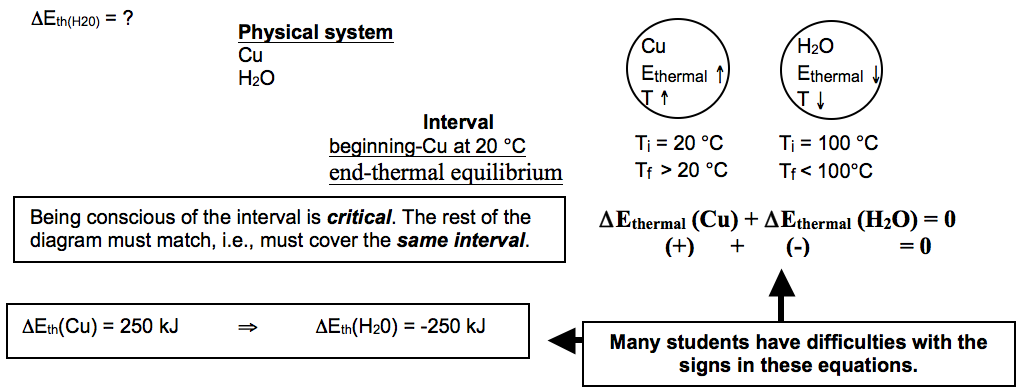
\includegraphics[width=\linewidth]{act116-b}
	}
	
\WCD

	\note{}{
		Do any clarifying that is necessary, but try to get the students to do most of the explaining. 
		
		At the end of this whole-class discussion, ask the question: ``Why was it necessary to ask part (b) after part (a) and not vice-versa?''
		
		Answer: To apply the \EnergyInteractionModel{} you have to know what energy systems are involved.  In this particular case, that means knowing whether or not there will be a phase change of either of the substances.  
	}
	
	\item Redraw your \TempGraphs{} for the new initial conditions. Explain briefly how you could determine if the \ce{H2O} will undergo a phase change or temperature change.
	
	\note{The students will need to be able to do this kind of analysis in DLM03!}{
		\todo[inline]{What is this reference to DLM03 in DLM4 using future tense about?}
		Help them figure out that they need to compare the magnitude of energy needed to increase the temperature of the Cu to 100$^\circ$C with the magnitude of energy lost by the \ce{H2O} as it completes its phase change to decide if the \ce{H2O} will change temperature.
		\begin{itemize}
			\item If the former is smaller, when the Cu reaches 100$^\circ$C the \ce{H2O} will only be partway through its phase change, and the process will stop (thermal equilibrium). 
			\item If the former is larger, the \ce{H2O} will complete its phase change before the Cu reaches 100$^\circ$, and the process will continue until thermal equilibrium is reached. 
		\end{itemize}
	}
\end{enumerate}

\WCD

\note{}{
	Try to get the students to do most of the explaining, but make sure all of the important points are covered.
}
	\newpage
%We're taking the following activity out for now and maybe will come back to it later if time permits
%	\section[Energy in Chemical Reactions]{Applying the \EnergyInteractionModel{} to Chemical Reactions}
\label{act1.1.7}

\begin{overview}

\noindent
{\bfseries Overview:} Now that we've used the \EnergyInteractionModel{} to understand a few physical phenomena, we'll apply it to understand a class of phenomena that you might already be familiar with from chemistry: Chemical reactions.

\end{overview}

\note{Purpose}{
	Students think about what bond energy means in the context of chemical reactions, instead of phase changes.
}

\begin{fnt}
	\label{fnt1.1.4-1}

Every general model is applicable to some range of physical phenomena. The \EnergyInteractionModel{} can be used to analyze $v_i$rtually {\em any} process, but up to this point we have been using it to make sense of the phenomena of {\em temperature changes} and {\em phase changes}. The former are modeled as changes in thermal energy systems, with the indicator being temperature, and the latter are modeled as changes in bond energy systems, with the indicator being the mass of substance that is changing phase. But {\em bond energy} changes in chemical reactions just as it does in phase changes, so we use exactly the same approach when modeling chemical reactions.

Consider the following chemical reaction, the hydration of calcium sulfate (Plaster of Paris). Recall that when you mix water with the white power, the paste not only gets hard, but it also gets hot:
\begin{center}
\ce{(Ca2SO4)2 * \ce{H2O} + 3\ce{H2O} -> 2Ca2SO4 * 2\ce{H2O} + Heat_{to~env.}}
\end{center}
Has the bond energy of this \textbf{\em total} system increased, decreased, or stayed the same during this process (mixing water with the powder)?  Use the \EnergyInteractionModel{} to explain. The simplest way to answer this question is to model all of these different chemicals as being a {\em single} physical system with {\em one} thermal-energy system and {\em one} bond-energy system. (Note that the question asked about the {\em total bond energy}, not bond energies of the separate molecular species. If the question had asked about bond energy changes of particular molecular species, we would have to include separate bond energies in our model.)



\end{fnt}

\noindent The chemical reaction that occurs when you mix together powdered Plaster of Paris and water resulting in a paste that can be used for molds and casts as it solidifies is given by:			
\begin{center}
	\ce{(Ca2SO4)2 * \ce{\ce{\ce{H2O}}} + 3\ce{\ce{\ce{H2O}}} -> 2 (Ca2SO4 * 2\ce{\ce{\ce{H2O}}}) + $Q$_{to~env.}}
\end{center}
Represent this process in an \EnergyDiagram{} by modeling {\em all} of the reactants and products {\em together} as having a {\em single} bond energy system and a single {\em thermal} energy system. \textbf{Assume the initial and final temperatures are the same} and that heat ($Q$) has been transferred to the environment during the process, which is obvious if you have ever mixed Plaster of Paris. This should make answering the question asked in \hyperref[fnt1.1.4-1]{the FNT} (``Did the bond energy increase, decrease, or stay the same?'') very straightforward.

\note{}{
	Since heat was produced, the total bond energy must have decreased.
}

\WCD 

\begin{fnt}
	\label{fnt1.1.4-2}

\begin{enumerate}[(a)]
	\item Think about the general case of chemical reactions. When a single compound breaks up into separated atoms, what can you say with absolute certainty regarding the \textbf{\em change} in bond energy of that compound? Why? What can you say with absolute certainty regarding the change in bond energy of a compound that is formed from separated constituent atoms? Why?
	
	\item Consider this chemical reaction: the combustion of propane.
	\begin{center}
		\ce{C3 H8 + 5 O2  ->  3 CO2 + 4 \ce{H2O}}
	\end{center}
	We can model this process as if the reactant molecules are broken down into their constituent atoms, which are then re-assembled into the product compounds.

	\begin{enumerate}[i.]
		\item Represent this process with an \EnergyDiagram{} that contains four separate bond energy systems, one for each molecular species. There will be one for the \ce{C3 H8}, one for the \ce{5 O2}, etc.
	
		\item Using your result from part (a), show the direction of each bond energy change with an arrow in the standard way. The indicator for each compound is the number of moles of that compound.
		
		\item Show the initial and final values of each of the indicators in the standard way.
	\end{enumerate}
	
	\item The magnitude of the bond energy changes for all the molecules involved in this process when they are separated into atoms are:

	\begin{center}
	\ce{C3 H8}: \unitfrac[4002]{kJ}{mol}; \;
	\ce{O2}: \unitfrac[495]{kJ}{mol}; \; 
	\ce{CO2}: \unitfrac[1607]{kJ}{mol}; \;
	\ce{H2O}: \unitfrac[925]{kJ}{mol}.
	\end{center}
	
	\begin{enumerate}[i.]
		\item Determine the bond energy changes, the $\Delta E_\text{bond}$, for each of the reactants and products.
		\item Write a conservation of energy equation in the standard way  ($\Delta E_1 + \Delta E_2 + \Delta E_3 + \Delta E_4 = Q$). Write this equation out with appropriate subscripts to clearly identify each term.
		\item Rewrite it with the numerical values being careful to get the algebraic sign correct.
		\item Calculate $Q$, which will be the heat released from the combustion of one mole of propane.
		\item Is the algebraic sign of $Q$ that you calculate consistent with our sign convention for $Q$?
	\end{enumerate}
\end{enumerate}
\end{fnt}

\noindent
We'll now use the \EnergyInteractionModel{} to get a close approximation of the heat of combustion of a mole of propane in a chemical reaction. This is an example of how our general approach to energy conservation using the \textbf{\EnergyInteractionModel{}} encompasses topics that traditionally seem to be something entirely different; e.g., the heat of combustion of various chemical substances.

\begin{enumerate}
	\item Discuss briefly in your group your responses to question (a) regarding what you can say with certainty about changes in bond energy. Come to a consensus and \textbf{put your response on the board}.
	
	\note{}{
		When a compound breaks up into constituent atoms, its bond energy increases. 
	
		When a compound is formed, its bond energy decreases.
	}
	
	\item Share your responses to part (b) in your group and put an \EnergyDiagram{} up on the board as directed in part (b) of \hyperref[fnt1.1.4-1]{the FNT}. Make sure everyone in your group understands why the values of the indicators are the way they are. Make sure the difference in the values of the indicators between reactants and products makes sense to everyone in your group and why the changes are in the direction shown on your diagram.
	
	\note{}{
		There should be four bond energy systems:
			\begin{itemize}
				\item \ce{C3H8} bond energy increases as bonds break.
				\item \ce{O2} bond energy increases as bonds break.
				\item \ce{CO2} bond energy decreases as bonds form. 
				\item \ce{\ce{\ce{\ce{H2O}}}} bond energy decreases as bonds form.
			\end{itemize}
	}
	
	\item Write your equation expressing energy conservation with the appropriate numerical values to show how to find $Q$.
	
	\note{}{
		\begin{align*}
		\Delta E_{\text{bond} (\ce{C3H8})} + \Delta E_{\text{bond} (\ce{O2})} + \Delta E_{\text{bond} (\ce{CO2})} +\Delta E_{\text{bond} (\ce{\ce{\ce{\ce{H2O}}}})} \&= Q\\
		\unitfrac[4002]{kJ}{mol} + 5(\unitfrac[495]{kJ}{mol}) - 3(\unitfrac[1607]{kJ}{mol}) - 4(\unitfrac[92]{kJ}{mol}) \&= -\unit[2044]{kJ}
		\end{align*}
	}
\end{enumerate}

\note{Note for Instructor}{
	In their introductory chemistry course students will have been introduced to various ``Heats'' expressed as $\Delta H$'s:  Heat of formation, heat of fusion, heat of vaporization, etc. In this FNT, values of the various $\Delta E_\text{bond}$'s were calculated by looking up in a chemistry text the heats of formation of the different molecules. The algebraic signs can be confusing, but thinking about it in terms of how a particular $\Delta E$ changes, you canr $KE$ep it straight. The other confusing thing about using heats of formation, is that the ``zero'' is typically taken to be the state of the element at STP. So, for example, the heat of formation of \ce{O2} is typically listed as zero, but the atomic \ce{O} does have a listed value. Also note that all values of heats of formation, other heats, and heat capacities are listed in chemistry books or tables typically shown as $\Delta H$'s. This is because enthalpy, $H$, is the appropriate energy to use when processes are carried out at constant pressure. This all becomes clear at the end of the quarter when we do some simple thermodynamics.
	\todo[inline]{The last sentence of this paragraph is false and may require updating.}
}

\WCD  
\note{}{
	Aside from summing up and clarifying, a point that is good for you to emphasize is that this is what they were doing in their chemistry class with heats of formation. This is all the same science!  Whether we call it chemistry or physics, it is the same fundamental thing!  Many students really think that physics energy is somehow different from chemistry energy.
}
%	\newpage
	%Making this a subsection because it's still about practicing the models...
\subsection{Thermal and Bond Energy Systems}
\label{act1.2.2}

\begin{fnt}
	\label{fnt1.2.1-1}

Consider again the phenomenon of two substances at different temperatures exchanging energy as they come to thermal equilibrium: \emph{Substance A} and \emph{Substance B}, at initially different temperatures, are placed in contact. They are able to exchange energy as heat, and they can only exchange it with each other. Substance A has a greater initial temperature than Substance B. No phase changes occur during this process.

Use the \EnergyInteractionModel{} to create a logical explanation that unequivocally shows that the following statement about the heat exchange described above for Substances A and B is true or that it is false:

\begin{quote}
	``The energy that is transferred as heat to or from the object with the larger heat capacity must be greater than the energy that is transferred as heat to or from the object with the smaller heat capacity.''
\end{quote}
\end{fnt}

\note{Timing: \unit[\textless3]{min}}{
	\begin{itemize}
		\item The answer may be obvious, but make them explain how they know in the WC discussion. For example, ``With only two energy systems, the magnitude of energy leaving the one must be the same as the magnitude of energy into the second.'' As always, it is important for them to put things into their own words. 
		\item Follow-up question: Ask them what the effect of the different heat capacities will be.
	\end{itemize}
}

\noindent Discuss this FNT in your group and be prepared to explain in the whole class discussion. You do not need to put anything on the board.

\WCD

\begin{fnt}
	\label{fnt1.2.1-2}

Consider the following example of two substances at different temperatures exchanging heat as they come to thermal equilibrium.

A \unit[3.50]{kg} piece of lead and a \unit[1.5]{kg} piece of aluminum, at different temperatures, are placed in contact. They are able to exchange energy as heat and they can only exchange it with each other. The initial temperature of the lead is \unit[48]{\textdegree C}, and the initial temperature of the aluminum is \unit[35]{\textdegree C}. The table on page 5 the course notes has phase change temperatures and values of specific heats for these substances. 

\begin{enumerate}[(a)]
	\item If it is possible (How do you know this?), construct a single, closed \EnergyDiagram{} for the process of lead and aluminum coming to thermal equilibrium.

	\item Write an algebraic expression of energy conservation in terms of the $\Delta E$s of the two energy systems, and then substitute in the appropriate expressions for the $\Delta E$s.

	\item Substitute in all known numerical values. How many unknowns are there in your equation expressing energy conservation?

	\item At an {\em intermediate} point in the entire process described above the lead has reached a temperature of \unit[43]{\textdegree C}.
	
	Follow the instructions for part (a) for the interval that \emph{ends when the lead is at a temperature of \unit[43]{\textdegree C}}. What feature related to the process connects the final temperatures of lead and aluminum that appear in your diagram to each other?

\end{enumerate}
\end{fnt}

\note{Timing: \unit[$\sim$15]{min}}{
	\subsubsection*{What is the purpose of Handout 1.2.2?  (distributed to students)}
	\begin{itemize}
		\item Save time in today's DL. None of the diagrams in the handout needs to be put on the board by students or instructors. 
		\item Everyone has uniform conventions for \EnergyDiagrams{}. 
		\item Illustrates what is appropriate to put on the board for WC discussion. 
		\begin{itemize}
			\item It is not useful to show the algebraic manipulations necessary to get the final answer on the board. Make it clear that in the future, only what is shown in this diagram is what they should put on the board for the WC discussion.
			\item Discourage the students from working out the algebra in class. We want them to understand the difference between ``the physics'', which is illustrated in the diagrams on the handout, and ``the algebra''.
		\end{itemize}
	\end{itemize}
}


\begin{enumerate}[1.]
	\item A student constructed the following \EnergyDiagram{} for part (a) of \hyperref[fnt1.2.1-2]{this FNT}:

	\includegraphics[width=0.7\linewidth]{handout-fnt121-2a}
	
	Discuss the diagram briefly in your group, and identify any questions you have. You don't need to put anything on the board.\footnote{Incidentally, this diagram illustrates how much algebra is useful to put down for the purpose of clear communication in whole class discussions. In general, it is not useful to show the details of solving the algebra on the board. Being able to construct the correct diagram and getting the first three lines of algebra (including verifying the signs of the terms in the third line) are worth most of the credit on an exam.}
	
	\note{}{
		Students inspect diagram for part (a) on the handout and identify any questions. Not necessary to put anything on the board.
		
		If they have questions about the diagram you can respond either to the SG individually, or if you think others might benefit, with the WC. 
	}
	
	\item Put a complete \EnergyDiagram{} on the board for the shorter interval described in part (d) of \hyperref[fnt1.2.1-2]{this FNT}. What specifically is happening in the process that ``connects'' the two final temperatures (of lead and aluminum) in your diagram? Illustrate this on the board with two separate \TempGraphs{}, one for each substance.
	
	\note{}{
		Put a complete \EnergyDiagram{} on the board for the {\em shorter} interval described in part (d). What is the connection between the two final temperatures in your diagram? 
		\begin{itemize}
			\item The \EnergyDiagram{} is shown directly below.
			\item The connection: the two indicators are correlated with the end of the interval, i.e., they have those values at the same time. This may seem obvious to the point of being trivial, but as the number of terms in the equation expressing energy conservation increases, students have more difficulty seeing the relationship among the various initial and final values.
		\end{itemize}
	}
	
	\note{}{
		\noindent
		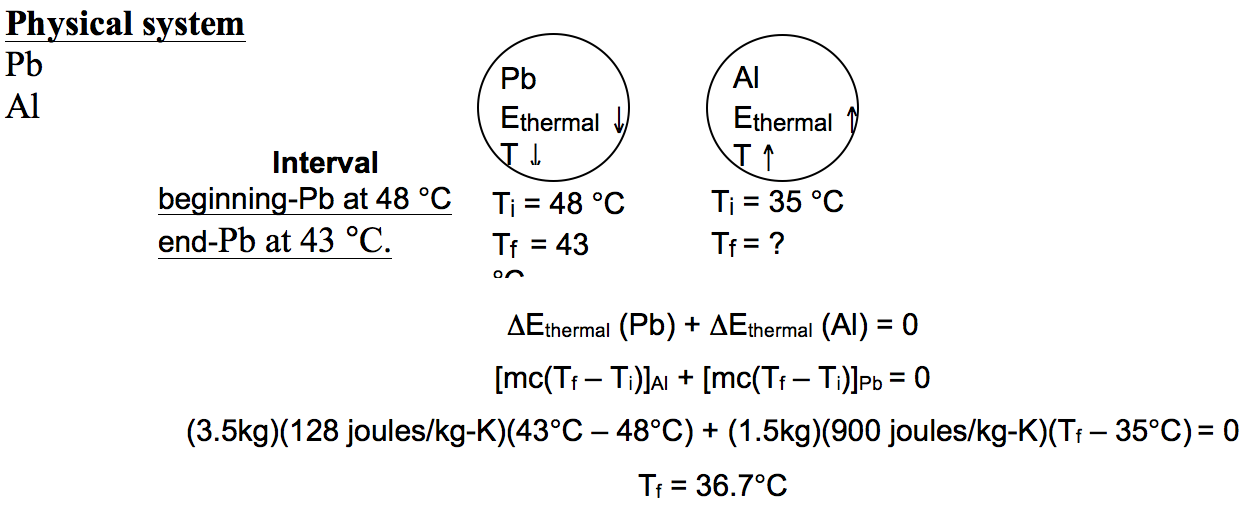
\includegraphics[width=\linewidth]{fnt121-2b}
	}

\WCD 

\end{enumerate}

\begin{fnt}
	\label{fnt1.2.1-3}

Suppose you used a hot pot to convert a \unit[150]{g} piece of ice that was initially at \unit[-15]{\textdegree C} into liquid water at \unit[50]{\textdegree C}.

\begin{enumerate}[(a)]
	\item Represent this process in two complete \EnergyDiagrams{}, one covering the interval from \unit[-15]{\textdegree C} to \unit[0]{\textdegree C} liquid, and the second covering the interval from \unit[0]{\textdegree C} liquid to \unit[50]{\textdegree C}.
	\item Now represent the entire process in one complete \EnergyDiagram{} covering the entire interval.
	\item If your hot pot has a power rating of \unit[600]{watts}, show how to find how long it will take to complete the process. (Make sure you are comfortable using standard units of energy, and that you understand the relation of power to energy.)
\end{enumerate}
\end{fnt}

\note{Timing: \unit[\about10]{min}}{
	
}

\begin{enumerate}[1.]

	\item Again, we consider a student's response to \hyperref[fnt1.2.1-3]{this FNT}. Discuss the diagrams for part (a) below and identify any questions you have. As before, you don't have to put anything on the board for this part.
	
		\includegraphics[width=0.55\linewidth]{handout-fnt121-3a1}
		\;
		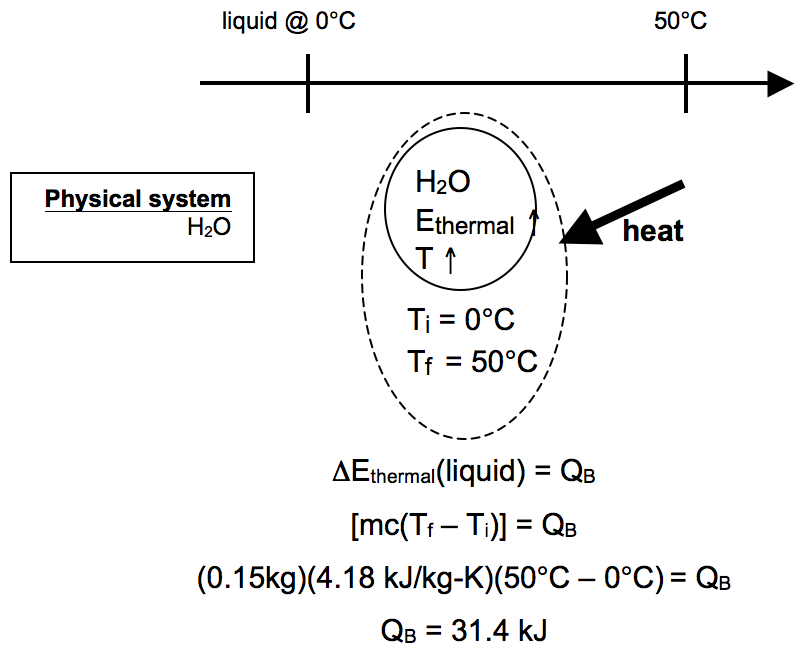
\includegraphics[width=0.35\linewidth]{handout-fnt121-3a2}
	
	\item A student objects to the diagram for part (b) of \hyperref[fnt1.2.1-3]{this FNT} below because some of the indicators do not correspond to the beginning and end of the overall interval.
	
		\includegraphics[width=0.7\linewidth]{handout-fnt121-3b}
		
		Another student says that's ok because each physical process in the interval happens sequentially and nothing has been left out. Come to a consensus about which of these two students you agree with and put a brief explanation on the board.
	
	\item Discuss the question about power in part (c) in your group and identify any questions you have. Make sure you have a clear understanding of the relationship of power to energy. You don't have to put anything on the board for part (c), but be ready to explain the difference between energy and power if called upon in the whole class discussion.

\WCD

\end{enumerate}

\subsection{Asking Questions and Determining Intervals of Interest}
\label{act1.2.2D}

\begin{fnt}
	\label{fnt1.2.1-4}

\ref{fnt1.2.1-2} and \ref{fnt1.2.1-3} emphasized the significance of the beginning and end of the interval -- we've called them ``initial'' and ``final'' states so far. This FNT illustrates
\begin{enumerate}[(i)]

	\item that the question you're asking determines the interval being analyzed with the \EnergyInteractionModel{}; and

	\item that sometimes it's necessary to adjust the size of the interval in order to be able to use the model.

\end{enumerate}

\noindent The physical process we want to analyze with the \ThreePhaseModel{} and the \EnergyInteractionModel{} is the following:\\

\noindent Imagine you are using your hot pot to gradually add heat to a \unit[500]{g} block of ice that has just been removed from a freezer with an internal temperature of \unit[-25]{\textdegree C}. The hot pot is fairly well insulated, so it is reasonable to assume that all of the heat put into the pot from the electrical heater located in the bottom of the pot goes into the \ce{H2O}. We can also assume that the heat capacity of the pot is much smaller than the heat capacity of \unit[500]{g} of \ce{H2O} (whether solid or liquid), so we can ignore the thermal energy system of the pot itself.

One question we could ask is, ``What is the final state of the water (phase and temperature) after the addition of \unit[252]{kJ} of heat?'' 

\begin{enumerate}[(a)]

	\item Explain why -- based {\em only} on the given information and without further analysis or calculation -- it is \textbf{\em not possible} to construct a {\em single} \EnergyDiagram{} that could be used to determine the final state of the water.
	
		[Hint: try to construct such a diagram. Another way to think about this is whether you can define the final state so that it depends on only one variable without making unjustified assumptions?]

	\item In cases like this, you must first use the model to analyze a {\em shorter interval}. Can you construct an \EnergyDiagram{} that could be used to determine how much energy is needed to increase the temperature of the ice to \unit[0]{\textdegree C}?
	
		Now explain in a few sentences how to proceed using the \EnergyInteractionModel{} to find the final state of the \ce{H2O}.

\end{enumerate}
\end{fnt}

\note{Timing: \unit[\about10]{min}}{
	
}

\begin{enumerate}[1.]

	\item Why is it \emph{not} possible to apply the \textbf{\EnergyInteractionModel{}} in a {\em straightforward} way to the interval of interest -- the interval that ends when all of the \unit[252]{kJ} has been added to the water? In other words, why can't the overall interval be diagrammed using {\em only} the given information prior to doing any further analysis?   Draw a \TempGraph{} to help you make sense of this and to use to explain it. In particular, be sure to make explicit which part of the graph in the diagram refers to which ``energy bubble'' on the \EnergyDiagram{}. [To save time, it is ok for explanations on the board to be more abbreviated than explanations on exams because anything that is unclear can be easily clarified in the whole class discussion.]
	
	\item Explain how to use the \textbf{\EnergyInteractionModel{}} to analyze shorter intervals in order to determine the final state (phase and temperature) of the water.  (Note: ``water,'' without a modifier, usually means \ce{H2O} in any one of its Three-Phases.) Use a \TempGraph{} in your analysis and to use in your explanation.

\WCD 

\end{enumerate}
	\newpage
%Taking out the handout because the images were incorporated into Act1.2.2
%	\section{Handout for \hyperref[act1.2.2]{Activity\about\ref*{act1.2.2}}}

\subsection*{\ref{fnt1.2.1-2}(a)}

\noindent
\includegraphics[width=0.7\linewidth]{U1/figs/handout-fnt121-2a}

\subsection*{\ref{fnt1.2.1-3}(a)}

\noindent
\includegraphics[width=0.55\linewidth]{U1/figs/handout-fnt121-3a1}
\;
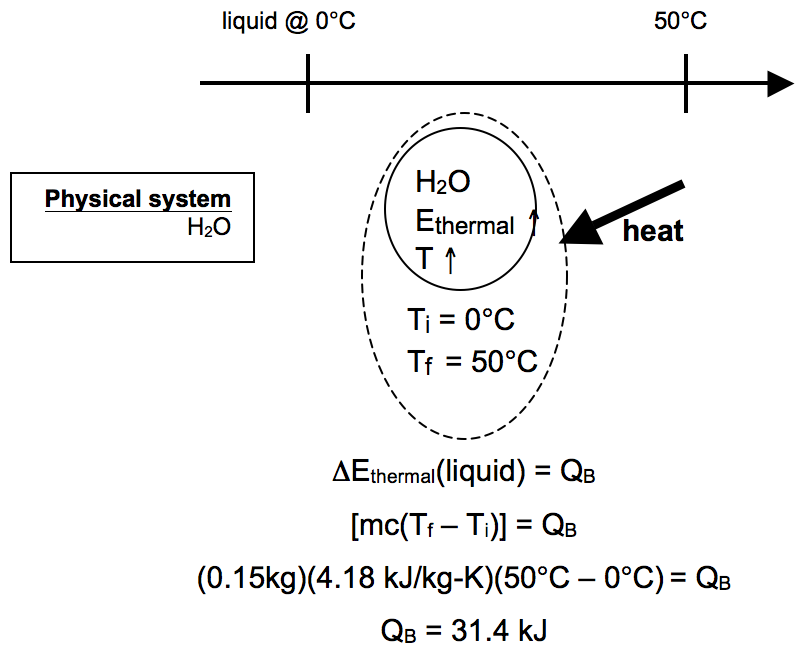
\includegraphics[width=0.35\linewidth]{U1/figs/handout-fnt121-3a2}

\subsection*{\ref{fnt1.2.1-3}(b)}

\noindent
\includegraphics[width=0.7\linewidth]{U1/figs/handout-fnt121-3b}


%%%%%%%%%%%%%%%%%%%%%%%%%%%%%%%%%%%%%%%%%%%%%%%%%%%%%%%%%%%%%%%%%%%%%%%%
%
%		DLM 5A
%
%%%%%%%%%%%%%%%%%%%%%%%%%%%%%%%%%%%%%%%%%%%%%%%%%%%%%%%%%%%%%%%%%%%%%%%%

\chapter[\chaptername\thechapter]{\chapterlongname \thechapter}
\label{dlm5a}
\addchapter

	\section{More Practice with the \EnergyInteractionModel{}}
\label{act1.1.8}

\begin{overview}

	\textbf{Overview:} We continue our efforts to practice using our models -- particularly the \EnergyInteractionModel{} -- by investigating new phenomena.
	
\end{overview}

\subsection{Cooling Water Below its Freezing Point}

\begin{fnt}
	\label{fnt1.1.4-3}

Perhaps you recall that when table salt, \ce{NaCl}, is added to water, the freezing point of water is lowered. Consider a system composed of a mixture of \unit[2.5]{kg} of ice and \unit[50]{g} of liquid water and a small, separate container of finely powdered salt. This physical system is contained in a fully insulated container that prevents all thermal interactions with the environment. Both the salt and the ice-water mixture are initially at the freezing point of water, \unit[0]{\textdegree C}. The salt is then added to the ice-water mixture, and the system of ice-water and salt is allowed to come to thermal equilibrium. The final equilibrium temperature is less than \unit[0]{\textdegree C}.\\

Use the \EnergyInteractionModel{} to predict if there will be a greater or lesser amount of ice in the final equilibrium state than in the initial state before the salt was added. Your explanation should include a complete \EnergyDiagram{}.\\

[The simplest way to model this physical system is with one thermal energy system for everything and one bond energy system, i.e., in terms of the model, it is not useful to distinguish between the various chemical components in order to answer this particular question.]
\end{fnt}

\note{Timing: \unit[\textless3]{min}}{
%Note:  You will have done these FNTs BEFORE coming to class, so you have only a few minutes (\unit[\textless3]{min}) to work on these together in your group.	
}

\noindent On the board, construct the simplest \EnergyDiagram{} that represents a particular model of the process described in this FNT. 

Make sure everyone in your group is ready to explain which elements of your completed diagram represent information that was given, or known, and which elements you had to infer, based on given or known information and the logic of the model? 

\WCD  

\begin{fnt}
	\label{fnt1.1.4-4}

\todo[inline]{FNT 1.1.4-4) change to thought experiment and we will do in class}

This FNT is a \textbf{\emph{thought experiment}} to make predictions about an actual experiment we will do in class, where you will get to observe the phenomenon described in \ref{fnt1.1.4-3}.\\

Imagine you fill an insulated cup almost full with chopped or crushed ice, and measure the temperature after a minute or two, once it's all come to thermal equilibrium. Since this ice is frozen water, the temperature should be at \unit[0]{\textdegree C} or not more than a couple of degrees below. Then, imagine you add a bunch of salt and stir it around. 

What do you think the lowest temperature you can attain will be? Why? What happens to the amount of liquid present if your keep stirring and adding salt? How can we understand this phenomenon in terms of thermal and bond energy systems?

Develop an explanation for the changes you would observe in this physical system (decrease in temperature and change of phase) in terms of the \EnergyInteractionModel{}.
\end{fnt}

\note{Timing: \unit[\textless3]{min}}{
	
}

\noindent Now we'll actually do this experiment:

\begin{enumerate}

	\item On your table, you have an insulated mug and a thermometer. Get some ice from the ice chest on the counter and fill your insulated mug. Measure the temperature inside the ice-filled cup and verify it is at around \unit[0]{\textdegree C}.

	\item Now, add some salt and stir it into the ice with a stirrer (don't use the thermometer; it might break!). Measure the temperature of the salt-ice mixture inside the cup. Add some more salt and repeat the stirring and temperature measurement. How far can you get the temperature to drop?

	\item On the board, list the low temperatures attained by your group.

\end{enumerate}

\noindent Would the following statement be something that would be good to memorize?

\begin{quote}
	{\em ``When bond energy increases, thermal energy must decrease, and vice versa.''}
\end{quote}

\noindent Explain on the board why it would or would not be good to memorize this.

\WCD  

\subsection{Heating Water with Microwaves}

\begin{fnt}
	\label{fnt1.2.1-5}

\todo[inline]{1.2.1-5) print FNT doesn't match Canvas FNT - change instructor notes to cover canvas FNT}

%\subsubsection*{Print Version}

%Use your insulated cup (and some larger microwaveable container, if available) and your thermometer to determine the effective ``cooking power'' of a microwave oven for different amounts of water. Try to use 4 or 5 different amounts of water spread over as wide a range of volumes as possible. [from a few tens of cubic centimeters (cc) to 5000 or more]. Use what you know about the thermal properties of water to design an experiment to test how much energy is transferred to the water in a given amount of time. From this measurement you can determine the actual power, in watts, that the microwave delivers to the water. This will typically not be the same for different amounts of water, so you should make measurements using different amounts. How does the maximum ``cooking power'' you measure compare to the electrical power the microwave uses (printed on the back of your microwave in watts)? Based on your data, what amounts of water corresponded to the most efficient use of electrical power?

%A microwave oven works by converting electrical energy to microwaves. Some of the energy in the microwaves is absorbed by the food/liquid placed in the oven. In terms of energy systems this means that the energy in the microwave system decreases and the thermal energy in the liquid/food increases. However, not all of the energy in the microwaves gets absorbed by the food/liquid. You are going to determine how much of the energy used by the microwave actually goes into heating your food.


%\subsubsection*{Canvas Version}

This is an actual experiment that you should perform at home:\\

\noindent Put approximately 1 cup of cold water in a microwave safe dish (Tupperware, drinking glass, etc.), measure the temperature (you can use a thermometer you would use to measure your body temperature), then heat it for a set period of time (somewhere between 30 seconds and a minute will work well). When you take the water out, measure the temperature again.

\begin{enumerate}[(a)]
	\item Draw an \EnergyDiagram{} for the water in your cup, and determine the change in thermal energy of the water. Convert this to Watts (a unit of power).
	
	\item Compare the number of Watts you determined in part a) to the power rating listed on the microwave information plate (usually located on the back of the oven, but you can always look up the model online). Which is greater? What does this mean?
	
	\item Where might the energy go if it is not heating up the food?
	
	\item Does the percentage of energy going to the food depend on the amount of water? You might choose a small amount, say half a cup, and a large amount, say two cups to investigate this question.
\end{enumerate}
\end{fnt}

\note{Timing: \unit[\textless3]{min}}{
	
}

\noindent On the board, choose the data from a member of your group, and sketch a graph of cooking power vs.\ amount of water. 

You'll notice that there appears to be some ``missing power.'' That is, the difference in power actually used to heat the water is less than the power used by the unit as stated on a label on the back of the microwave unit.

{[}\textbf{Hint:} Can you feel or hear anything near the back of the microwave unit when it is turned on?{]}

\WCD  

%Not a new activity...
%	\newpage
	%Not making this a section because it's really just more practice and should be a part of the previous activity
%\section[Quantitative Applications of the Model]{Quantitative Applications of the \EnergyInteractionModel{}}
\label{act1.2.4}

\note{

	\begin{itemize}
		\item Groups 1 - 3 discuss and respond to \ref{fnt1.2.1-6} as directed below.
		\item Groups 4 - 6 discuss and respond to \ref{fnt1.2.1-7} as directed below.
	\end{itemize}

}

\subsection{Boiling Liquid Nitrogen with Ice}  

\begin{fnt}
	\label{fnt1.2.1-6}

A \unit[2.2]{kg} block of ice (\ce{H2O}) initially at a temperature of \unit[-20]{\textdegree C} is immersed in a \emph{very large} amount of liquid nitrogen (\ce{N2}) at a temperature of \unit[-196]{\textdegree C}. The \ce{N2} and \ce{H2O} are allowed to come to thermal equilibrium.  [T$_\text{BP(\ce{N2})}$ = \unit[-196]{\textdegree C}]

Create a particular model of this process and use it to determine how much liquid \ce{N2} is converted to gas (vapor).

[Hint: The emphasis on ``very large'' implies that there will still be liquid \ce{N2} left when the two come to thermal equilibrium.]
\end{fnt}

\note{Timing: \unit[\about10]{min}}{
	
}

\begin{enumerate}
	\item There exits a definite correlation between each energy system in your \EnergyDiagram{} and each $\Delta E$ term in your energy conservation equation. In addition to ensuring that you include all the appropriate $\Delta E$'s (and no extra ones) in your algebraic equation expressing conservation of energy, what other very important detail can your \EnergyDiagram{} tell you about each $\Delta E$ term in your equation?
	
	\item Construct a complete \EnergyDiagram{} (including an algebraic statement of energy conservation in terms of the $\Delta E$'s) for this process. Then rewrite the equation expressing energy conservation substituting in the appropriate expressions for changes in energy of the energy systems using variables only (no numbers). \textbf{Do not substitute any numbers for the variables, and do not solve for the unknown, but circle the unknown variable in the equation.} Put the algebraic sign in parentheses above each algebraic term in the algebraic equation.

	We know you know how to do simple algebra and arithmetic. However, the most common mistake students often make is in the algebraic sign of the whole term when subtracting \emph{initial} values from \emph{final} values of the indicators. By using the \EnergyDiagram{} to check that the sign is correct, you will avoid making this error.\footnote{Just for reference: You likely found that \about\unit[4]{kg} of liquid \ce{N2} was converted to vapor.}

\end{enumerate}

\subsection{Warming Ice with Liquid Water}  

\begin{fnt}
	\label{fnt1.2.1-7}

The \unit[2.2]{kg} block of ice from the \ref{fnt1.2.1-6} is eventually removed from the liquid \ce{N2} (after reaching thermal equilibrium with the liquid \ce{N2}) and placed in a {\em very large} amount of liquid \ce{H2O} at \unit[0]{\textdegree C}, where it comes to thermal equilibrium with the liquid \ce{H2O}. Create a particular model of this process and use it to determine the final mass of the ice.
\end{fnt}

\note{Timing: \unit[\about10]{min}}{}

\begin{enumerate}
	\item Describe in words what is going on in this process, specifically: What physical system is changing phase? What system is changing temperature? What energy systems need to be included in the particular model you create for this process?
	
	\item Construct a complete \EnergyDiagram{} (including an algebraic statement of energy conservation in terms of the $\Delta E$'s) for this process. Then rewrite the equation that expresses energy conservation, substituting in the appropriate expressions for changes in energy of the energy systems using variables only (no numbers). \textbf{Do not substitute any numbers for the variables, and do not solve for the unknown,} but circle the unknown variable in the equation.\footnote{Again, for reference: You likely got a final mass of ice of \about\unit[5]{kg}.}

\WCD

\end{enumerate}

\subsection{Melting Gold}

\begin{fnt}
	\label{fnt1.2.1-8}

\unit[2.0]{kg} of solid gold (\ce{Au}) at an initial temperature of \unit[1000]{K} is allowed to exchange heat with \unit[1.5]{kg} of {\em liquid} gold at an initial temperature of \unit[1336]{K}. The solid and liquid can only exchange heat with each other. When the two reach thermal equilibrium, will the mixture be entirely solid, or will there be a mixed solid/liquid phase? {\em Explain how you know.}

\end{fnt}

\note{Timing: \unit[\textless5]{min}}{
	
}

\noindent Discuss in your group and make sure everyone is prepared to explain your group's response in the whole class discussion.

\WCD

	\newpage
	%\section{Manipulating the Interval}

%Changing this to just be the ice-tea activity
\section{Defining Appropriate Intervals for Analysis}
\label{act1.2.3}

\begin{overview}

\textbf{Overview:} Remember that we \hyperref[act1.2.2D]{talked about} how asking different questions makes us choose different intervals of interest for our investigations using the \EnergyInteractionModel? Here, we'll explore this issue a bit further.

\end{overview}

% We already did this activity and FNT in D/L 4. Commenting this out here.
%\subsection{}
%
%\begin{fnt}
%	\label{fnt1.2.1-4}

\ref{fnt1.2.1-2} and \ref{fnt1.2.1-3} emphasized the significance of the beginning and end of the interval -- we've called them ``initial'' and ``final'' states so far. This FNT illustrates
\begin{enumerate}[(i)]

	\item that the question you're asking determines the interval being analyzed with the \EnergyInteractionModel{}; and

	\item that sometimes it's necessary to adjust the size of the interval in order to be able to use the model.

\end{enumerate}

\noindent The physical process we want to analyze with the \ThreePhaseModel{} and the \EnergyInteractionModel{} is the following:\\

\noindent Imagine you are using your hot pot to gradually add heat to a \unit[500]{g} block of ice that has just been removed from a freezer with an internal temperature of \unit[-25]{\textdegree C}. The hot pot is fairly well insulated, so it is reasonable to assume that all of the heat put into the pot from the electrical heater located in the bottom of the pot goes into the \ce{H2O}. We can also assume that the heat capacity of the pot is much smaller than the heat capacity of \unit[500]{g} of \ce{H2O} (whether solid or liquid), so we can ignore the thermal energy system of the pot itself.

One question we could ask is, ``What is the final state of the water (phase and temperature) after the addition of \unit[252]{kJ} of heat?'' 

\begin{enumerate}[(a)]

	\item Explain why -- based {\em only} on the given information and without further analysis or calculation -- it is \textbf{\em not possible} to construct a {\em single} \EnergyDiagram{} that could be used to determine the final state of the water.
	
		[Hint: try to construct such a diagram. Another way to think about this is whether you can define the final state so that it depends on only one variable without making unjustified assumptions?]

	\item In cases like this, you must first use the model to analyze a {\em shorter interval}. Can you construct an \EnergyDiagram{} that could be used to determine how much energy is needed to increase the temperature of the ice to \unit[0]{\textdegree C}?
	
		Now explain in a few sentences how to proceed using the \EnergyInteractionModel{} to find the final state of the \ce{H2O}.

\end{enumerate}
%\end{fnt}

%\note{Timing: \unit[\about10]{min}}{
	
%}

%\begin{enumerate}
%	\item Why is it {\em not} possible to apply the \textbf{\EnergyInteractionModel{}} in a straightforward way to the interval of interest? (The interval that ends when all of the \unit[252]{kJ} has been added to the water.) In other words, why can't the overall interval be diagrammed using {\em only} the given information prior to doing any further analysis?   Draw a \TempGraph{} to help you make sense of this and to use to explain it. In particular, be sure to make explicit which part of the graph in the diagram refers to which ``energy bubble'' on the \EnergyDiagram{}. \textbf{[To save time, it is ok for explanations on the board to be more fragmentary and shorthand than explanations on exams, because anything that is unclear can be easily clarified in the Whole Class Discussion.]}
	
%	\item Explain how to use the \EnergyInteractionModel{} to analyze {\em shorter intervals} in order to determine the final state (phase and temperature) of the \ce{H2O}. Use a \TempGraph{} in your analysis and to use in your explanation.
%\end{enumerate}

%\WCD 

%\subsection{Two objects coming to thermal equilibrium}
\todo[inline]{Notes on Ice-Tea activity

	Needs to be restructured as chart addition doesn't fit well. Perhaps do original ice tea activity and THEN do chart if time?}

\noindent\textbf{Consider the following phenomenon:} A \textbf{big} chunk of ice (water) at an initial temperature of  \unit[65]{\textdegree C} is placed inside a well-insulated container with some tea at an initial temperature of \unit[20]{\textdegree C}, and the two are allowed to come to thermal equilibrium. (The tea can be treated as water with respect to thermal properties.)

\begin{enumerate}
	\item There are several possible final states of this process. We will be using and reusing the same \ThreePhaseModel{} to determine possible final states. Draw two \TempGraphs{}, one for tea and one for \ce{H2O}.
	\begin{enumerate}
		\item Why can't either substance reach thermal equilibrium in the gaseous phase nor the mixed (liquid/gas) phase nor the gaseous phase?
		\item Using the \hyperref[act123-grid]{grid below}, your instructor will assign your group one of the potentially possible final states. Trace your \TempGraph{} to show how your assigned ending phase is or is not possible.
		\label{act123-gridprob}
	\end{enumerate}

\newcommand{\gridsize}{3cm}
\begin{table}[h]
	\caption{Grid for \ref{act123-gridprob}}
	\label{act123-grid}
	\begin{tabular}{cr>{\centering}b{\gridsize}>{\centering}b{\gridsize}b{\gridsize}<{\centering}}
							&						& \multicolumn{3}{c}{\textbf{Tea}} \\
							&						& Solid 						& Mixed Phase\newline\scriptsize(Solid/Liquid) & Liquid \\\cline{3-5}
							&						& \multicolumn{1}{|l|}{i.} 			& \multicolumn{1}{|l|}{ii.}	& \multicolumn{1}{|l|}{iii.} \\
							& 						& \multicolumn{1}{|c|}{} 			& \multicolumn{1}{|c|}{}	& \multicolumn{1}{|c|}{} \\
							& Solid					& \multicolumn{1}{|c|}{} 			& \multicolumn{1}{|c|}{}	& \multicolumn{1}{|c|}{} \\
							& 						& \multicolumn{1}{|c|}{} 			& \multicolumn{1}{|c|}{}	& \multicolumn{1}{|c|}{} \\
							& 						& \multicolumn{1}{|c|}{} 			& \multicolumn{1}{|c|}{} 	& \multicolumn{1}{|c|}{} \\\cline{3-5}
							&  						& \multicolumn{1}{|l|}{iv.} 			& \multicolumn{1}{|l|}{v.}	& \multicolumn{1}{|l|}{vi.} \\
\multirow{3}{*}{\rotatebox[origin=l]{90}{\textbf{Ice}}}	& 	 		& \multicolumn{1}{|c|}{}			& \multicolumn{1}{|c|}{} 	& \multicolumn{1}{|c|}{} \\
							& Mixed Phase				& \multicolumn{1}{|c|}{} 			& \multicolumn{1}{|c|}{}	& \multicolumn{1}{|c|}{} \\
							& \scriptsize(Solid/Liquid)		& \multicolumn{1}{|c|}{} 			& \multicolumn{1}{|c|}{}	& \multicolumn{1}{|c|}{} \\
							&  						& \multicolumn{1}{|c|}{} 			& \multicolumn{1}{|c|}{}	& \multicolumn{1}{|c|}{} \\\cline{3-5}
							&  						& \multicolumn{1}{|l|}{vii.} 			& \multicolumn{1}{|l|}{viii.}	& \multicolumn{1}{|l|}{ix.} \\
							& 	 					& \multicolumn{1}{|c|}{} 			& \multicolumn{1}{|c|}{}	& \multicolumn{1}{|c|}{} \\
							& Liquid					& \multicolumn{1}{|c|}{} 			& \multicolumn{1}{|c|}{}	& \multicolumn{1}{|c|}{} \\
							&  						& \multicolumn{1}{|c|}{} 			& \multicolumn{1}{|c|}{}	& \multicolumn{1}{|c|}{} \\
							&  						& \multicolumn{1}{|c|}{} 			& \multicolumn{1}{|c|}{}	& \multicolumn{1}{|c|}{} \\\cline{3-5}
	\end{tabular} 
\end{table}


\WCD

	\item Now that we have a class consensus on which states are possible, your instructor will assign you one of the possible final states:
	\begin{enumerate}
		\item For your possible final state, draw an \EnergyDiagram{} (with energy conservation equation, as always).
		\item Would your final state be possible if there were A LOT of ice?  What about with A LOT of tea?

\WCD

	\end{enumerate}

	\bitem{Thinking about how to proceed:  How do we determine the final state?}
	
	Put a \TempGraph{} on the board for each of the two systems: The water that starts out as ice at \unit[-65]{\textdegree C} and the tea (liquid water) that starts out at \unit[20]{\textdegree C}. Put a big dot on each graph at the initial state.
	
	\begin{enumerate}
		\item Have two separate group members place a finger on the two starting dots. Then a third group member should start explaining how energy is transferred from one physical system to the other, specifically naming the energy systems that are losing energy and that are gaining energy. Move the fingers along each graph in response to the explanation. Make sure every group member agrees with the explanation and the motion along the graphs. STOP when one substance gets to a phase change temperature.
		
		\item We need to use quantitative skills to figure out \textbf{which substance gets to its phase change temperature first}. With your group members, think about ways that you might be able to determine this. Hint: Are there two values you can compare? Write in words what you need to do to figure this out.
		\label{act123-compare-energies}
		
		\item After you have explained in words how you will figure out which substance gets to its phase change first, draw an \EnergyDiagram for each calculation you want to perform, and then perform the calculation.

\WCD 

		\item Is it possible to determine the final state of the substances yet?  Is it possible to eliminate any of the possible final states? Which one(s)?
		
		\item We now need to repeat \hyperref[act123-compare-energies]{Part~\ref*{act123-compare-energies}} to figure out which happens first: the tea decreases to \unit[0]{\textdegree C},  or the ice goes through an entire phase change. Draw {\em NEW initial points} and determine which changes in energy you need to compare. Then draw the \EnergyDiagrams, and do the calculations.
		
		\item Are the two physical systems in thermal equilibrium at the end of this step?  How do you know this?
		
		\item Can you now determine the final state of the ice and tea system? Draw an appropriate \EnergyDiagram on the board for this. If you finish early, you may solve for the final temperature or state.

\WCD

	\end{enumerate}
\end{enumerate}
	
\part{Mechanical Energy Systems}
\label{Unit2}
	
	%%%%%%%%%%%%%%%%%%%%%%%%%%%%%%%%%%%%%%%%%%%%%%%%%%%%%%%%%%%%%%%%%%%%%%%%
%
%		DLM 5B
%
%%%%%%%%%%%%%%%%%%%%%%%%%%%%%%%%%%%%%%%%%%%%%%%%%%%%%%%%%%%%%%%%%%%%%%%%

\chapter[\chaptername\thechapter]{\chapterlongname \thechapter}
\label{dlm5b}
\addchapter

%	%\section{Manipulating the Interval}

%Changing this to just be the ice-tea activity
\section{Defining Appropriate Intervals for Analysis}
\label{act1.2.3}

\begin{overview}

\textbf{Overview:} Remember that we \hyperref[act1.2.2D]{talked about} how asking different questions makes us choose different intervals of interest for our investigations using the \EnergyInteractionModel? Here, we'll explore this issue a bit further.

\end{overview}

% We already did this activity and FNT in D/L 4. Commenting this out here.
%\subsection{}
%
%\begin{fnt}
%	\label{fnt1.2.1-4}

\ref{fnt1.2.1-2} and \ref{fnt1.2.1-3} emphasized the significance of the beginning and end of the interval -- we've called them ``initial'' and ``final'' states so far. This FNT illustrates
\begin{enumerate}[(i)]

	\item that the question you're asking determines the interval being analyzed with the \EnergyInteractionModel{}; and

	\item that sometimes it's necessary to adjust the size of the interval in order to be able to use the model.

\end{enumerate}

\noindent The physical process we want to analyze with the \ThreePhaseModel{} and the \EnergyInteractionModel{} is the following:\\

\noindent Imagine you are using your hot pot to gradually add heat to a \unit[500]{g} block of ice that has just been removed from a freezer with an internal temperature of \unit[-25]{\textdegree C}. The hot pot is fairly well insulated, so it is reasonable to assume that all of the heat put into the pot from the electrical heater located in the bottom of the pot goes into the \ce{H2O}. We can also assume that the heat capacity of the pot is much smaller than the heat capacity of \unit[500]{g} of \ce{H2O} (whether solid or liquid), so we can ignore the thermal energy system of the pot itself.

One question we could ask is, ``What is the final state of the water (phase and temperature) after the addition of \unit[252]{kJ} of heat?'' 

\begin{enumerate}[(a)]

	\item Explain why -- based {\em only} on the given information and without further analysis or calculation -- it is \textbf{\em not possible} to construct a {\em single} \EnergyDiagram{} that could be used to determine the final state of the water.
	
		[Hint: try to construct such a diagram. Another way to think about this is whether you can define the final state so that it depends on only one variable without making unjustified assumptions?]

	\item In cases like this, you must first use the model to analyze a {\em shorter interval}. Can you construct an \EnergyDiagram{} that could be used to determine how much energy is needed to increase the temperature of the ice to \unit[0]{\textdegree C}?
	
		Now explain in a few sentences how to proceed using the \EnergyInteractionModel{} to find the final state of the \ce{H2O}.

\end{enumerate}
%\end{fnt}

%\note{Timing: \unit[\about10]{min}}{
	
%}

%\begin{enumerate}
%	\item Why is it {\em not} possible to apply the \textbf{\EnergyInteractionModel{}} in a straightforward way to the interval of interest? (The interval that ends when all of the \unit[252]{kJ} has been added to the water.) In other words, why can't the overall interval be diagrammed using {\em only} the given information prior to doing any further analysis?   Draw a \TempGraph{} to help you make sense of this and to use to explain it. In particular, be sure to make explicit which part of the graph in the diagram refers to which ``energy bubble'' on the \EnergyDiagram{}. \textbf{[To save time, it is ok for explanations on the board to be more fragmentary and shorthand than explanations on exams, because anything that is unclear can be easily clarified in the Whole Class Discussion.]}
	
%	\item Explain how to use the \EnergyInteractionModel{} to analyze {\em shorter intervals} in order to determine the final state (phase and temperature) of the \ce{H2O}. Use a \TempGraph{} in your analysis and to use in your explanation.
%\end{enumerate}

%\WCD 

%\subsection{Two objects coming to thermal equilibrium}
\todo[inline]{Notes on Ice-Tea activity

	Needs to be restructured as chart addition doesn't fit well. Perhaps do original ice tea activity and THEN do chart if time?}

\noindent\textbf{Consider the following phenomenon:} A \textbf{big} chunk of ice (water) at an initial temperature of  \unit[65]{\textdegree C} is placed inside a well-insulated container with some tea at an initial temperature of \unit[20]{\textdegree C}, and the two are allowed to come to thermal equilibrium. (The tea can be treated as water with respect to thermal properties.)

\begin{enumerate}
	\item There are several possible final states of this process. We will be using and reusing the same \ThreePhaseModel{} to determine possible final states. Draw two \TempGraphs{}, one for tea and one for \ce{H2O}.
	\begin{enumerate}
		\item Why can't either substance reach thermal equilibrium in the gaseous phase nor the mixed (liquid/gas) phase nor the gaseous phase?
		\item Using the \hyperref[act123-grid]{grid below}, your instructor will assign your group one of the potentially possible final states. Trace your \TempGraph{} to show how your assigned ending phase is or is not possible.
		\label{act123-gridprob}
	\end{enumerate}

\newcommand{\gridsize}{3cm}
\begin{table}[h]
	\caption{Grid for \ref{act123-gridprob}}
	\label{act123-grid}
	\begin{tabular}{cr>{\centering}b{\gridsize}>{\centering}b{\gridsize}b{\gridsize}<{\centering}}
							&						& \multicolumn{3}{c}{\textbf{Tea}} \\
							&						& Solid 						& Mixed Phase\newline\scriptsize(Solid/Liquid) & Liquid \\\cline{3-5}
							&						& \multicolumn{1}{|l|}{i.} 			& \multicolumn{1}{|l|}{ii.}	& \multicolumn{1}{|l|}{iii.} \\
							& 						& \multicolumn{1}{|c|}{} 			& \multicolumn{1}{|c|}{}	& \multicolumn{1}{|c|}{} \\
							& Solid					& \multicolumn{1}{|c|}{} 			& \multicolumn{1}{|c|}{}	& \multicolumn{1}{|c|}{} \\
							& 						& \multicolumn{1}{|c|}{} 			& \multicolumn{1}{|c|}{}	& \multicolumn{1}{|c|}{} \\
							& 						& \multicolumn{1}{|c|}{} 			& \multicolumn{1}{|c|}{} 	& \multicolumn{1}{|c|}{} \\\cline{3-5}
							&  						& \multicolumn{1}{|l|}{iv.} 			& \multicolumn{1}{|l|}{v.}	& \multicolumn{1}{|l|}{vi.} \\
\multirow{3}{*}{\rotatebox[origin=l]{90}{\textbf{Ice}}}	& 	 		& \multicolumn{1}{|c|}{}			& \multicolumn{1}{|c|}{} 	& \multicolumn{1}{|c|}{} \\
							& Mixed Phase				& \multicolumn{1}{|c|}{} 			& \multicolumn{1}{|c|}{}	& \multicolumn{1}{|c|}{} \\
							& \scriptsize(Solid/Liquid)		& \multicolumn{1}{|c|}{} 			& \multicolumn{1}{|c|}{}	& \multicolumn{1}{|c|}{} \\
							&  						& \multicolumn{1}{|c|}{} 			& \multicolumn{1}{|c|}{}	& \multicolumn{1}{|c|}{} \\\cline{3-5}
							&  						& \multicolumn{1}{|l|}{vii.} 			& \multicolumn{1}{|l|}{viii.}	& \multicolumn{1}{|l|}{ix.} \\
							& 	 					& \multicolumn{1}{|c|}{} 			& \multicolumn{1}{|c|}{}	& \multicolumn{1}{|c|}{} \\
							& Liquid					& \multicolumn{1}{|c|}{} 			& \multicolumn{1}{|c|}{}	& \multicolumn{1}{|c|}{} \\
							&  						& \multicolumn{1}{|c|}{} 			& \multicolumn{1}{|c|}{}	& \multicolumn{1}{|c|}{} \\
							&  						& \multicolumn{1}{|c|}{} 			& \multicolumn{1}{|c|}{}	& \multicolumn{1}{|c|}{} \\\cline{3-5}
	\end{tabular} 
\end{table}


\WCD

	\item Now that we have a class consensus on which states are possible, your instructor will assign you one of the possible final states:
	\begin{enumerate}
		\item For your possible final state, draw an \EnergyDiagram{} (with energy conservation equation, as always).
		\item Would your final state be possible if there were A LOT of ice?  What about with A LOT of tea?

\WCD

	\end{enumerate}

	\bitem{Thinking about how to proceed:  How do we determine the final state?}
	
	Put a \TempGraph{} on the board for each of the two systems: The water that starts out as ice at \unit[-65]{\textdegree C} and the tea (liquid water) that starts out at \unit[20]{\textdegree C}. Put a big dot on each graph at the initial state.
	
	\begin{enumerate}
		\item Have two separate group members place a finger on the two starting dots. Then a third group member should start explaining how energy is transferred from one physical system to the other, specifically naming the energy systems that are losing energy and that are gaining energy. Move the fingers along each graph in response to the explanation. Make sure every group member agrees with the explanation and the motion along the graphs. STOP when one substance gets to a phase change temperature.
		
		\item We need to use quantitative skills to figure out \textbf{which substance gets to its phase change temperature first}. With your group members, think about ways that you might be able to determine this. Hint: Are there two values you can compare? Write in words what you need to do to figure this out.
		\label{act123-compare-energies}
		
		\item After you have explained in words how you will figure out which substance gets to its phase change first, draw an \EnergyDiagram for each calculation you want to perform, and then perform the calculation.

\WCD 

		\item Is it possible to determine the final state of the substances yet?  Is it possible to eliminate any of the possible final states? Which one(s)?
		
		\item We now need to repeat \hyperref[act123-compare-energies]{Part~\ref*{act123-compare-energies}} to figure out which happens first: the tea decreases to \unit[0]{\textdegree C},  or the ice goes through an entire phase change. Draw {\em NEW initial points} and determine which changes in energy you need to compare. Then draw the \EnergyDiagrams, and do the calculations.
		
		\item Are the two physical systems in thermal equilibrium at the end of this step?  How do you know this?
		
		\item Can you now determine the final state of the ice and tea system? Draw an appropriate \EnergyDiagram on the board for this. If you finish early, you may solve for the final temperature or state.

\WCD

	\end{enumerate}
\end{enumerate}
%	\newpage
	\section{Modeling with Mechanical Energy Systems}
\label{act2.1.1}

\begin{overview}

\textbf{Overview:} After spending the first few weeks of the semester discussing and making sense of various \emph{thermal} phenomena, we now shift our focus to \emph{mechanical} phenomena. We'll start with some new definitions and then immediately dive into some examples.
	
\end{overview}

\subsection{Internal Energy and Mechanical Energy}

\begin{reading}

\noindent At this point, it is useful to define and distinguish two different \emph{types} of energy systems. Make sure the definitions make sense to everybody in your group!\\

\noindent\textbf{Internal Energy}:  Internal energy systems are closely related to the {\em motions} of and {\em relationships} between {\em individual atoms and molecules}. Thermal Energy and Bond Energy are examples of internal energy systems.\\

\noindent\textbf{Mechanical Energy}: Mechanical energy systems have {\em indicators} involving the {\em position} or the {\em speed} of the {\em object as a whole}.  The object can be anything from an airplane to an atom.\\

\noindent\textbf{Important}: Some physical phenomena (such as the thermal phenomena we've dealt with, so far) involve changes {\em only} in internal energy systems, while some phenomena involve changes \emph{only} in mechanical energy systems. Other phenomena involve changes in \emph{both} mechanical and internal energy systems.
\end{reading}

\WCD 

\subsection{Phenomenon: Dropping a golf ball}

Drop a golf ball from about one meter above the floor and observe its motion and position.  Focus on the motion and position between the \textbf{beginning} and \textbf{end} states defined below. If you do not have names of energy systems associated with the changes you observed, you can just make up names for these energy systems for now.

\begin{center}
\begin{tikzpicture}
    % draw horizontal line   
    \draw[->] (0,0) -- (10,0);

    % draw vertical lines
    \foreach \x in {0.5,9.5}
      \draw (\x cm,3pt) -- (\x cm,-3pt);

    % draw nodes
    \draw (0.5,0) node[below=3pt] {\emph{just as} ball is released} node[above=3pt] {\emph{beginning}};
    \draw (9.5,0) node[below=3pt] {\emph{just before} ball hits the floor} node[above=3pt] {\emph{end}};
\end{tikzpicture}
\end{center}

\begin{enumerate}
	\item Write on the board: What properties of the physical system (indicators) do you think change \textbf{significantly} between the initial and final state?  What energy systems are associated with those indicators?  Are these \emph{internal} or \emph{mechanical} energy systems, or both?
	\item Put a complete \EnergyDiagram{} on the board.  Show with an arrow if each energy system increases or decreases. Include initial and final values of the indicators.
	\item Write an algebraic representation of your \EnergyDiagram{} that expresses energy conservation in terms of the changes of energy of the relevant energy systems.  
\end{enumerate}

\WCD 

\subsection{Phenomenon: Dropping a coffee filter}

Drop a basket type coffee filter from a height of about two meters.  Release it oriented as shown in the figure.

\begin{center}
	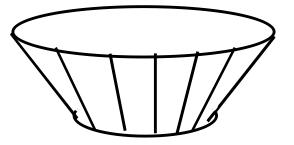
\includegraphics[width=0.25\textwidth]{act211-coffeefilter}

\begin{tikzpicture}
    % draw horizontal line   
    \draw[->] (0,0) -- (10,0);

    % draw vertical lines
    \foreach \x in {0.5,9.5}
      \draw (\x cm,3pt) -- (\x cm,-3pt);

    % draw nodes
    \draw (0.5,0) node[below=3pt] {\emph{\textbf{one second} after} filter is released} node[above=3pt] {\emph{beginning}};
    \draw (9.5,0) node[below=3pt] {\emph{just before} filter hits the floor} node[above=3pt] {\emph{end}};
\end{tikzpicture}
\end{center}

\begin{enumerate}
	\item Repeat part 1 above. Don't forget the last part of the question!
	\item Repeat parts 2 and 3 above.

\WCD 

\subsubsection*{Discuss in your group:}
	
	\item Which of the energy systems you have identified depend on only the \emph{magnitude} of the indicator and which depend on {\em both} the \emph{magnitude} and the \emph{sign} associated with that indicator? 
	\item How are your {\em particular models} for the golf ball and coffee filter different from each other?  Be specific.  What physical properties of the objects are responsible for this difference?
	
\end{enumerate}

\WCD 
	\newpage
	\section{A New Construct and A New Model}
\label{act2.1.2}

\begin{overview}
\textbf{Overview:} A third mechanical energy system -- in addition to \emph{translational kinetic} energy $KE_\text{translational}$ and \emph{gravitational potential} energy $PE_\text{gravity}$ -- is the \emph{spring-mass} energy $PE_\text{spring-mass}$, introduced here in the context of the \SOModel{}.
\end{overview}

\subsection{Oscillating Spring-Mass}

Many physical systems oscillate. The spring-mass system that you are going to examine is one example of many such systems that can be modeled using the \SOModel{}.

\begin{enumerate}
	\item Hang a \unit[200]{g} mass on the spring. The equilibrium position of the mass is the location of the mass when the system is at rest. Use the two-meter stick with the pointer to mark the equilibrium position of the mass. Pull the mass down or push it up \textbf{a few centimeters} and release it. Describe the resulting motion of the mass (e.g., Where is it moving fastest? Where is its speed zero?).
	
	\item Does the resulting motion of the mass depend on whether you started the motion by \emph{lifting the mass up} a certain small distance (try \unit[\about1]{cm}) or by \emph{pulling it down} that same distance from its equilibrium (resting) position?
\end{enumerate}

\WCD

\subsection{Applying the \EnergyInteractionModel{}}
\label{act212.2}

\noindent Work out your responses to the questions below with your small group at the board. Remember that in order to identify an energy system, we need to have an indicator that tells us that the energy system is changing.\\

\noindent Start with the mass pulled down \unit[5]{cm} below its equilibrium position. 

\begin{center}
\begin{tikzpicture}
    % draw horizontal line   
    \draw[->] (0,0) -- (10,0);

    % draw vertical lines
    \foreach \x in {0.5,9.5}
      \draw (\x cm,3pt) -- (\x cm,-3pt);

    % draw nodes
    \draw (0.5,0) node[below=3pt] {\emph{just as} mass is released} node[above=3pt] {\emph{beginning}};
    \draw (9.5,0) node[below=3pt, align=center] {\emph{the instant} the mass passes\\through equilibrium position\\for the  \emph{first} time} node[above=3pt] {\emph{end}};
\end{tikzpicture}
\end{center}

\begin{enumerate}
	\item What {\em properties} of the physical system (indicators) changed significantly between the initial and final state?  What energy systems are associated with those indicators?
	\label{act212.2-3}
	
	\item Make a complete \EnergyDiagram{}:
	\label{act212.2-4}
		
	Show the increases and decreases in the energy systems and show the initial and final values of the indicator associated with each energy system -- be as explicit as possible.
	
	\item Write down an algebraic representation of your \EnergyDiagram, expressing energy conservation.

\end{enumerate}

\WCD  

\subsection{Reflecting on the \SOModel{}}

\begin{enumerate}
	\item Do changes in the energy systems you identified depend on the direction that the indicator changed (the sign of the indicator), or only on the magnitude of the indicator?
	
	\item Would the way you modeled this physical system be any different from what you did in your response to \hyperref[act212.2-4]{\ref*{act212.2}\#\ref*{act212.2-4}} if the \textbf{final state} were the instant the mass returned to its equilibrium position the second time, instead of the first?  How about if it were the 200th time?
\end{enumerate}

\WCD


%%%%%%%%%%%%%%%%%%%%%%%%%%%%%%%%%%%%%%%%%%%%%%%%%%%%%%%%%%%%%%%%%%%%%%%%
%
%		DLM 6
%
%%%%%%%%%%%%%%%%%%%%%%%%%%%%%%%%%%%%%%%%%%%%%%%%%%%%%%%%%%%%%%%%%%%%%%%%

\chapter[\chaptername\thechapter]{\chapterlongname \thechapter}
\label{dlm6}
\addchapter

	\section{Creating Particular Models with Mechanical Energies}
\label{act2.1.3}

\begin{overview}

\noindent\textbf{Overview:} The problems in this section illustrate how we can use the \EnergyInteractionModel{} to answer questions and make predictions about the allowed behavior of interacting objects that are difficult to approach in any other way.
	
\end{overview}


\subsection{Three Thrown Rocks}
\label{act2.1.3a}

\begin{fnt}
	Before we start with this problem, let's review what the \EnergyInteractionModel{} does for us. As we have said before, conservation of energy relates values of certain physical parameters at the beginning of a process to the values of those parameters at the end of the process. The parameters are typically the indicators of the energy systems that change during the process or interaction. If we have a question about -- or want to predict values for -- some parameter and this parameter happens to be an indicator of an energy system, or a coefficient in an expression for an energy system, then we can proceed to construct a particular model and see if it gets us what we want.\\

\begin{wrapfigure}{R}{.2\textwidth}
	\centering
	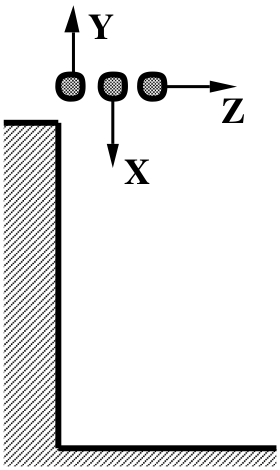
\includegraphics[width=.98\linewidth]{fnt211-rocksxyz}	
\end{wrapfigure}

\label{fnt2.1.1-1}

\noindent\textbf{The Phenomena}: Three rocks of equal mass are thrown with identical speeds from the top of the same building. (1) Rock X is thrown vertically downward, (2) Rock Y is thrown vertically upward, and (3) Rock Z is thrown horizontally.\\

\noindent\textbf{The Question}: Which rock has the greatest speed just before it hits the ground? Assume air resistance is negligible.\\

\noindent How can we determine this? We could take a guess, but it helps our argument if it is possible to apply the \EnergyInteractionModel{}. The prompts below will guide you through the process.

\begin{enumerate}[(a)]
	\item Let's start by making a prediction based on your prior experience. Don't waste a lot of time on this right now, but it's useful to give it some thought. We will definitely come back to this at the end in \hyperref[fnt211-1f]{Part~(\ref*{fnt211-1f})}. Your first, intuitive ideas might be very useful!
	\label{fnt211-1a}
	
	\item Does the question involve a parameter that you know to be an indicator of the change in an energy system? Which energy system and what is the indicator?
	\label{fnt211-1b}
	
	\item \textbf{Rock X}: Construct an \EnergyDiagram{} for Rock X, which is thrown straight down. Write out the expression for energy conservation, based on your \EnergyDiagram{}, as $\Delta E$'s; then substitute in algebraic symbols for the different energy systems. We are \emph{not} asking to go any further, but if you ``just have to,'' go ahead and try solving it for the final speed, $v_f$ (but you \emph{really} don't need to).
	\label{fnt211-1c}
	
	\item \textbf{Rock Y}: Now, without actually writing anything down, consider what would be different in your \EnergyDiagram{} for Rock Y. How about the algebraic representation -- anything different?  Go back and re-read the ``The Phenomena'' description at the beginning of the FNT, if you are not sure. Anything different in terms of what goes into the model? In terms of the \EnergyInteractionModel{} are there any differences?  Yes or No? Are you 100\% sure? Why?
	\label{fnt211-1d}
	
	\item \textbf{Rock Z}: Repeat for Rock Z. Any differences in the model?  Yes or No?
	\label{fnt211-1e}
	
	\item Do you believe that conservation of energy holds true for these three phenomena? Another way to ask this: Does the {\em particular energy model} you developed apply to all three cases?  If yes, what does conservation of energy tell you about the final \textbf{\em speeds} of the three rocks with 100\% confidence?
	\label{fnt211-1f}
	
	\item How do you reconcile your result in \hyperref[fnt211-1f]{Part~(\ref*{fnt211-1f})} with your initial ideas from \hyperref[fnt211-1a]{Part~(\ref*{fnt211-1a})} above?  They are not crazy, because there are indeed very obvious differences in the three situations. Why don't these differences matter to energy conservation?  Try to be as explicit here as you can be. This is what we will focus on in the FNT follow-up in DL.
	\label{fnt211-1g}
\end{enumerate}
\end{fnt}

\note{Timing: \unit[\textless20]{min}}{
	
}

\noindent Using the prompts below, \textbf{briefly} compare your group members' responses to \ref{fnt2.1.1-1} and put a short answer on your board (each letter corresponds to the same letter in the FNT):

\begin{enumerate}
	\item[\eqref{fnt211-1b}]	Does the \textbf{\em question} involve a parameter that you know to be an indicator of the change in an energy system?  Which energy system and what is the indicator?
	
	\item[\eqref{fnt211-1c}]	Draw an \EnergyDiagram{} for Rock X with an algebraic representation consisting of two and only two lines:
	\begin{enumerate}
		\item $1^{st}$ line, using $\Delta E$'s with subscripts.
		\item $2^{nd}$ line, substitute in algebraic expressions for each $\Delta E$.
	\end{enumerate}
	Do \textbf{NOT} solve for anything!
	
	\item[\eqref{fnt211-1d} \& \eqref{fnt211-1e}] Are there ANY differences in the \EnergyDiagrams{} for Rocks X, Y, and Z?
	
	\item[\eqref{fnt211-1f}] \begin{enumerate}[(i)]
		\item In terms of the {\em particular} model you have created for these phenomena (determined by which energy systems you included), what does your model predict with 100\% certainty about the final speed of each rock just before it hits the ground?
		\label{fnt211-1fi}
		
		\item In light of the dropping golf ball and coffee filter activity (\hyperref[act2.1.1]{Activity~\ref*{act2.1.1}}), what aspect of your model might have to be changed that could change your prediction regarding the final speeds of the ball?
		
		\item So, taking into account what you just determined in the previous two steps, what \emph{is} different about the final states of the balls?
	\end{enumerate}
	
	\item[\eqref{fnt211-1g}]	Discuss any intuitive ideas that different members of your group might've had that ``bug you the most,'' because they seem to contradict the \EnergyInteractionModel{}'s prediction that all rocks have the same final speed.
\end{enumerate}

\WCD\\

\begin{overview}
	\textbf{Check-In:} \emph{Does this all make sense to you?} In the context of this FNT, we discussed some very fundamental issues about energy conservation. If you're not sure about any of the above, please follow up with other students and/or your instructor during office hours. But before you do, carefully work through the entire FNT again!
\end{overview}

\subsection{Pulling up a Bucket}
\label{act2.1.3b}

\begin{fnt}
	\label{fnt2.1.1-2}

A person pulls a bucket of water up from a well using a rope. Assume that the initial and final speeds of the bucket are zero ($v_i=v_f=0$), and that the person lifted the bucket a vertical distance $h$. By looking at energy changes in the bucket-Earth physical system, we can make sense of the force the person must exert to pull the bucket up and determine the amount of work the person does.

\begin{enumerate}[(a)]
	\item Is the system open or closed? What energy systems undergo a change during this process? Construct an \EnergyDiagram{} and include the algebraic expression of energy conservation (in terms of $\Delta E$'s and, if open, any heat or work).
	
	\item Substitute the algebraic expression we use for the change in gravitational potential energy and solve algebraically for the work done by the person on the rope/bucket.
	
	\item Use the definition of work in terms of force and distance (refer to the \EnergyInteractionModel{} Summary) to find the average force exerted by the person on the rope and bucket while they are lifting it up.
\end{enumerate}


\end{fnt}

\note{Timing: \unit[\textless10]{min}}{
	
}

\begin{enumerate}
	\item Put on the board the algebraic expression you have for work in terms of energy changes. Be prepared to give an explanation that is both succinct and logically complete -- based on the \EnergyInteractionModel{} -- for how you know this expression is true.
	
	\item Substitute the expression for work in terms of force and distance moved (see \EnergyInteractionModel{} Summary), and solve for the force.
\end{enumerate}

\WCD
 
\subsection{Including the Potential Energy of a Spring}
\label{act2.1.3c}

\note{Timing: \unit[20]{min}}{
	
}

\begin{benumerate}
	\bitem{The Phenomenon}

	A toy car launcher works as follows:  There is a compressible spring that is attached to a horizontal rail, on which a toy car can roll. The toy car can be pushed back against the spring, compressing it a certain distance. There is a little hook that holds the car against the compressed spring. When the hook is released, the spring pushes the car out of the launcher, down the horizontal track.
	
\begin{center}
	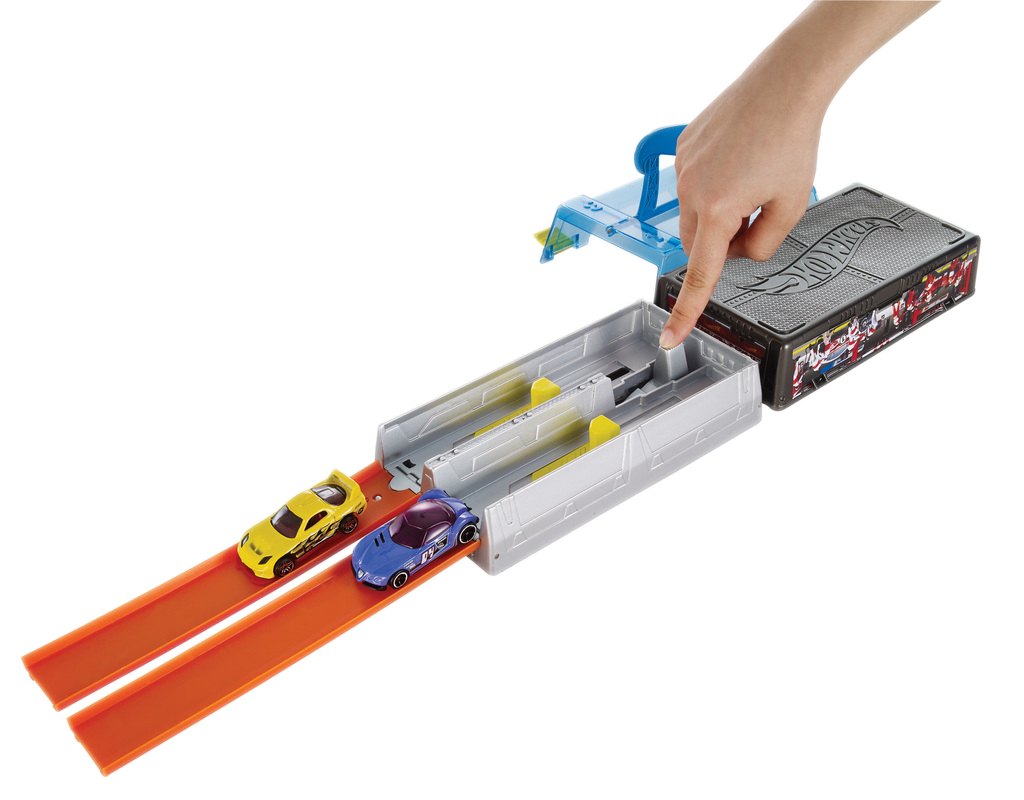
\includegraphics{act2.1.3c-toycarlauncher}	
\end{center}
	
	We want to ask some questions and make some predictions about different cars as they come out of the launcher.  Upon close examination of this launcher, it is noted that the spring is always compressed the same amount each time a car is loaded into the launcher. The spring stays put inside the launcher as the car is pushed out.

	\bitem{What we want to know or predict}
	
	\begin{itemize}
		\item Do all cars come out of the launcher with the same speed?  
		\item If they don't all have the same speed when they come out, what parameters cause the difference?
		\item What do we need to do to get our car to have a higher speed than our friend's cars?
	\end{itemize}
	
	\bitem{Create a Particular Model and Use it to answer the questions}

	Plan what you need to do in your group and how you will proceed BEFORE you start writing on the board.  Be systematic.  Then put your response on the board.	

	\bitem{Suggestions:}
	
	\begin{itemize}
		\item Use the \EnergyInteractionModel{} and the \SOModel{}.
		\item Consider what energy systems are involved.
		\item \textbf{Note:} The car is in contact with the spring while it is compressed and separates from the spring just as the spring reaches its equilibrium length. During the time that the car and spring are together, they behave as a spring-mass system.
		\item To simplify the notation, use ``$d$'' for the distance the spring is compressed instead of ``$\Delta x$''.
	\end{itemize}
	
	\bitem{Be prepared to present a precise, logical, explanation that ``gets at'' the answers to the questions.}
\end{benumerate}

\WCD
	\newpage
	\section{How We Use the \EnergyInteractionModel{}}
\label{act2.1.4}

\begin{overview}
	\textbf{Overview:} In this activity, we reflect on what we did when using the \EnergyInteractionModel{}. We'll generate some general guidelines for successful application of the model to make sense of physical phenomena.
\end{overview}


\subsection{Reflecting on Using the \EnergyInteractionModel{}}

In the previous activities we have been applying the \EnergyInteractionModel{} to a wide range of physical phenomena. Previously, we had applied it to thermal and chemical interactions. Here is a list of what we've just done with mechanical phenomena:

\begin{itemize}
	\item \hyperref[act2.1.1]{Activity~\ref*{act2.1.1}}	Dropped golf ball and dropped coffee filter
	\item \hyperref[act2.1.2]{Activity~\ref*{act2.1.2}}	Oscillating mass attached to a spring
	\item \hyperref[act2.1.3]{Activity~\ref*{act2.1.3}} \hyperref[act2.1.3a]{Three thrown rocks}, \hyperref[act2.1.3b]{Pulling up a bucket}, and \hyperref[act2.1.3c]{Toy car launcher}
\end{itemize}

\noindent In all of these cases we used the \EnergyInteractionModel{} to make sense of the phenomena, answer questions, make predictions, or develop explanations regarding the phenomena. But the \EnergyInteractionModel{} is a very general model that needs to be refined to tell us anything about the particular phenomena.

\begin{enumerate}
	\item What did you have to do and what decisions did you have to make in order to use/apply the \EnergyInteractionModel{}? There are \textbf{three} major decisions you must initially make that determine how you are modeling the process or phenomenon. The process of making an \EnergyDiagram{} helps you with this. List the most important three things you can think of here and on your board:
	\begin{enumerate}
		\item \hrulefill
		\item \hrulefill
		\item \hrulefill
	\end{enumerate}
	
	\item Which steps on the two-page blue model summary of the \EnergyInteractionModel{} do the above three steps correspond to? \hrulefill
\end{enumerate}
	
\noindent The process of making these decisions/choices is the \textbf{\em first step} in what we have and will continue to refer to as creating or developing a \textbf{\em particular model}. This is the model that can be directly applied to a particular phenomenon.

\WCD

\subsection{The Whole Process}

\begin{enumerate}
	\item To complete the creation of the particular model, you must do some more things, perhaps make some decisions. When first encountering a phenomenon, an \EnergyDiagram{} can be particularly useful because as you draw the diagram, you are forced to make these decisions.
	
	\item Create a particular model for the case of a mass hanging on a spring that is pulled down and released at a distance ``$d$'' below the point where the mass is hanging stationary. After the mass has completed a total of 10 complete oscillations, it is noticed that it didn't go quite as far down as the distance $d$. Put your particular model, in the form of a complete \EnergyDiagram{}, on the board. Be prepared to discuss in detail the decisions you had to make when forming this diagram.
	
	\item What are some of the questions that you could ask/answer or predictions you could make with this particular model? You would likely need to have more specific information that you could obtain from the phenomenon. Put these questions on the board with any additional information you would need.
\end{enumerate}

\WCD

\subsection{A New Phenomenon}

Imagine this situation: Two {\em identical} balls roll down two sets of slanted channels. The slope and length of the channels are the {\em same}, so the change in height is the same for both balls. However, the channels have different widths: one is wider than the other.

\begin{center}
	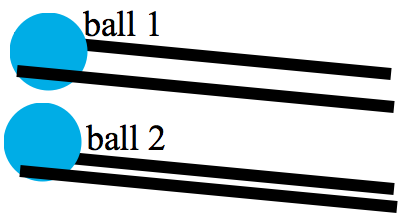
\includegraphics[width=0.25\textwidth]{act214-ramps}
\end{center}

\noindent Your instructor will give you two Pool balls. Let them roll down the channels -- starting them at the same time -- and observe what happens. Do this several times, carefully observing what is different about the way the balls roll. Could the difference be an indication that there is a new energy system that we need to take into account?

A maybe obvious question is, \textbf{\emph{``Why does one ball go faster and get to the bottom before the other ball?''}} Use the \EnergyInteractionModel{} to make sense of what is going on, and develop a succinct explanation with an appropriate \EnergyDiagram{} for why one of the balls gets to the bottom of the rails before the other ball.

\textbf{Note:} From careful measurements made on this apparatus, friction plays only a very small roll in the difference in speeds of the balls. You can safely assume that all frictional effects cause negligible energy changes compared to the changes in mechanical energies. 

\WCD
	\newpage
	\section{Quantitative Modeling of Mechanical Energies}
\label{act2.2.1}

\begin{overview}

	\textbf{Overview:} There are interesting features of some of the Mechanical Energy systems that only become apparent in the algebraic expression for the change in energy. These features can help us tremendously in making sense of physical phenomena. To remind you, the energy systems we are currently working with are $KE_\text{translational}$, $KE_\text{rotational}$, $PE_\text{gravity}$, $PE_\text{spring-mass}$, and $PE_\text{spring}$. In this activity, we will explore some quantitative features of these energy systems.
	
\end{overview}


\subsection{Relationships between Energy Systems and Indicators}

 In your small group, take a few minutes to think about and discuss {\em each} of the questions below. Each question will be followed immediately by a short \WCD

\begin{enumerate}
	\item What are the indicators of change in each of the Mechanical Energy systems?
	\item \begin{enumerate}
		\item Which of these energies depend on the square of the indicator and which depend on the first power of the indicator?
		\item Which of these energies depend on which direction something moves?
		\item What is the connection between the two previous questions?
	\end{enumerate}
	\item Which of these energy systems depend on the mass of the object and which depend on the weight? Why does this matter?
\end{enumerate}

\noindent
The fact that some indicators are linear and some are quadratic has additional consequences as the next two questions illustrate:

\begin{enumerate}\setcounter{enumi}{3}	
	\item Consider a heavy ball. Would it take the same amount of work to vertically lift it from \unit[25]{cm} to \unit[30]{cm} as it does to lift it from \unit[30]{cm} to \unit[35]{cm}? If not, which situation requires more work? Why?
	
	\item Does it take the same amount of work to speed your car up from \unitfrac[25]{m}{s} to \unitfrac[30]{m}{s} as it does to speed it up from \unitfrac[30]{m}{s} to \unitfrac[35]{m}{s}? If not, situation requires more work? Why?
\end{enumerate}

\subsection{Keeping Track of Directionality}
\label{act2.2.1b}

We are about to begin using the \EnergyInteractionModel{} to predict quantitative properties of various phenomena. A potential pitfall of quantitative modeling is that we sometimes tend to lose track of why we are doing something once we start calculating numbers. It is especially easy to lose track of \emph{directionality}, which is mathematically expressed in \emph{algebraic signs}. However, our \EnergyDiagrams{} tell us the signs of the various terms in the conservation of energy equation most of the time. Therefore, don't forget to use the \EnergyDiagrams{} to check the signs as you begin to model scenarios quantitatively!

\noindent\textbf{The Phenomenon:} Christine throws a ball straight up, letting go of the ball at a height of $y_i$ above the ground. When she lets go, the ball has an initial speed $v_i$. The ball travels straight up to its maximum height ($y_{max}$) and falls back down. Assume the frictional effects from air resistance are insignificant.

\subsubsection*{Constructing a particular model to find the maximum height:}

\begin{enumerate}
	\item Construct a particular model of this phenomenon that can be used to determine the maximum height of the ball. ($y_f = y_{max}$) Put a sketch of the path of the ball and a complete \EnergyDiagram{} (with accompanying energy conservation equation) on the board [leave half the board free for the following questions]. What do you know about the ball's speed at its maximum height when it's thrown straight up?
	
	\item Indicate the initial and final positions of the ball on your sketch that correspond to the initial and final conditions in your \EnergyDiagram{}.
	
	\item On the board, rewrite the energy conservation equation by replacing the two terms with algebraic expressions for the changes in energy of the energy systems. Does the resulting algebraic sign of each term in your energy conservation equation agree with the increases and decreases in energy systems in your diagrams?
	
	\item Solve the equation for ($y_f - y_i$). Does the sign of ($y_f - y_i$) make sense for this particular physical situation?
	\label{act2.2.1b4}
	
	\item If you knew the numerical value of $v_i$, could you calculate the maximum height?
\end{enumerate}

\WCD


%%%%%%%%%%%%%%%%%%%%%%%%%%%%%%%%%%%%%%%%%%%%%%%%%%%%%%%%%%%%%%%%%%%%%%%%
%
%		DLM 7A
%
%%%%%%%%%%%%%%%%%%%%%%%%%%%%%%%%%%%%%%%%%%%%%%%%%%%%%%%%%%%%%%%%%%%%%%%%

\renewcommand*\thesection{\thechapter}	%There's only one activity in this DL, so this will remove the letter from the activity number

\chapter[\chaptername\thechapter]{\chapterlongname \thechapter}
\label{dlm7a}
\addchapter

	\section[More Modeling with Mechanical Energy]{More Modeling of Scenarios involving Mechanical Energy Systems}
\label{act2.2.2}

\begin{overview}
	
	\textbf{Overview:} In this activity, we will explore additional scenarios that are related to phenomena we've already discussed. Here, we add some variations to the scenarios and answer some different questions we haven't asked yet.
	
\end{overview}

\noindent\textbf{Note:} Remember Christine throwing a ball in the air in \hyperref[act2.2.1b]{Activity~\ref*{act2.2.1b}}?

\begin{fnt}
	\label{fnt2.2.1-1}

If the initial upward speed of the ball in \hyperref[act2.2.1b]{Activity~\ref*{act2.2.1b}} is \unitfrac[10]{m}{s}, and the ball is released at a height of \unit[1.5]{m} above the floor, what is {\em the maximum height above the floor} that the ball reaches? How far \emph{above Christine's hand} is the ball when it reaches its maximum height, and how is this value related to your answer to \hyperref[act2.2.1b4]{\ref*{act2.2.1b4}} in \hyperref[act2.2.1b]{Activity~\ref*{act2.2.1b}}?
\end{fnt}

\begin{fnt}
	\label{fnt2.2.1-2}

\noindent With the same initial conditions as in \ref{fnt2.2.1-1}, use the \EnergyInteractionModel{} \textbf{\em in two different ways} to determine the speed of the ball when it is 4 meters above the floor, {\em headed down}:

\begin{enumerate}[(a)]
	\item Construct a particular model of {\em the entire physical process}, with the initial time when the ball leaves Christine's hand, and the final time when the ball is 4~meters above the floor, {\em headed down}.
	\item Divide the overall process into {\em two physical processes} by constructing two \EnergyDiagrams{} and applying energy conservation for each: one diagram for the interval corresponding to the ball traveling from Christine's hand to the maximum height; and one diagram corresponding to the interval for the ball traveling from the maximum height to 4 meters above the floor, {\em headed down}.
	\item Did you get different answers in parts (a) and (b) for the speed of the ball when it is 4 meters above the floor, {\em headed down}?
\end{enumerate}
\end{fnt}

\begin{fnt}
	\label{fnt2.2.1-3}

Use the \EnergyInteractionModel{} to show that an object thrown vertically upward will have the same speed as it comes down through any point that it had going up through that same point.

One way to do this is to construct two \EnergyDiagrams{}: One diagram should be from the point of release of the ball to some {\em intermediate} height as the ball is traveling upward, less than the {\em maximum} height; the second diagram should be from the point of release of the ball to that same intermediate height as the ball is on its way down. Then, compare the two diagrams. 
\end{fnt}

\begin{fnt}
	\label{fnt2.2.1-4}

In \hyperref[act2.2.1b]{Activity~\ref*{act2.2.1b}} we assumed that $y = 0$ at the level of the floor. If, instead, we assume that $y = 0$ where Christine releases the ball -- still 1.5~meters above the floor -- will this change the maximum height above the floor attained by the ball? Use the \EnergyInteractionModel{} to answer this question.
\end{fnt}

\noindent After throwing her ball in the air a few times, Christine is tired of playing with the ball and instead moves on to water balloons (much more fun, right?). She stands on top of the Science Building, ready to launch her water balloon.

\begin{fnt}
	\label{fnt2.2.1-5}

Christine drops a water balloon from the top of the Science Building. Let's assume that the balloon does not break when it strikes the ground. There are many questions we could ask about this situation. To answer any of them, it makes sense to model the Energy dynamics of the scenario first. Let's do that and then answer some particular questions!

\begin{enumerate}[(a)]
	\item \label{fnt2.2.1-5a} Create a particular model for this phenomenon by making an \EnergyDiagram{} for the process that takes place from the time the water balloon is dropped until it is motionless on the ground. Consider the indicators to determine what energy systems must be present/can be excluded. Have you included enough systems?
	\item If the water balloon falls a distance of \unit[21]{m}, what is the maximum temperature rise of the water balloon due to its being dropped? (Does you answer seem reasonable? Why or why not? It may help to check your units.)
	\item Is there anything that prohibits the water balloon from suddenly cooling off to its original temperature and leaping \unit[21]{m} into the air? From the random nature of thermal energy, why do you think we never see this happen? Respond {\em briefly}.
\end{enumerate}
\end{fnt}

\noindent Eventually, Christine grows tired of throwing and dropping things. She goes back into the Science Building to play with a mass that's hanging on a spring in one of the laboratory rooms.

\begin{fnt}
	\label{fnt2.2.1-6}

Christine's mass-spring system consists of a \unit[250]{g} mass hanging from a spring with a spring constant $k = \unitfrac[0.182]{J}{m^2}$. She pulls the mass down \unit[7.1]{cm} from its equilibrium position and then releases it from rest.

\begin{enumerate}[(a)]
	\item How much work did Christine do when she pulled the spring down from its equilibrium position? Assume that the mass was at rest before she pulled it down, and before it was released. (Use the \EnergyInteractionModel{}, {\em not} the expression $W = F_\text{avg} \cdot \Delta x$, to determine the work.)
	\label{fnt2.2.1-6a}
	\item Create a particular model (construct an \EnergyDiagram{}) for each of the following final conditions to predict the speed of the mass after it is released, and when it is:
	\label{fnt2.2.1-6b}
	\begin{enumerate}[(i)]
		\item moving up through the equilibrium position,
		\label{fnt2.2.1-6b1}
		\item moving down through equilibrium, and
		\label{fnt2.2.1-6b2}
		\item \unit[5.0]{cm} below the equilibrium position, moving down.
		\label{fnt2.2.1-6b3}
	\end{enumerate}
\end{enumerate}
\end{fnt}


\begin{center}\noindent\textbf{Each group is responsible for putting one of the following on the board.\\ Write so that all other groups can easily follow your presentation!}\end{center}


\noindent\framebox[1.1\width][c]{\textbf{Group 1}}\\

\noindent\ref{fnt2.2.1-1} \& \ref{fnt2.2.1-4} (\unit[\textless 5]{min}) 
 
 \begin{itemize}
 	\item[\textbf{Read:}] You should already have used the principle of energy conservation to develop an equation for the change in height of a ball thrown straight up in the air (from \hyperref[act2.2.1b]{Activity~\ref{act2.2.1b}}).
	
	\item[\textbf{Do:}] Write a sentence or two explaining what fundamental feature of the \EnergyInteractionModel{} ``accounts for'' why changing the location of $y = 0$ does not change your calculation of the ball's maximum height above the floor. [\textbf{Hint:} think about the general form of the algebraic expression of energy conservation.]
\end{itemize}

\noindent
\ref{fnt2.2.1-2} (\unit[\textless 5]{min})

\begin{itemize}
	\item[\textbf{Read:}] When you model the process described in \ref{fnt2.2.1-2} in two different ways, i.e., using an interval corresponding to the overall process in versus splitting the overall process into two contiguous pieces with separate intervals corresponding to each part, you should get the same result for the speed of the ball at \unit[4]{m} above the floor.
	
	Check with your instructor for the correct numerical answer.
	
	\item[\textbf{Do:}] In terms of the \EnergyInteractionModel{}, why is it not necessary to divide the overall process into two pieces in order to find the speed of the ball at \unit[4]{m} above the floor falling down? 		 
\end{itemize}


\noindent\framebox[1.1\width][c]{\textbf{Group 2}}\\

\noindent\ref{fnt2.2.1-3} (\unit[\textless 10]{min})\\

\noindent Construct one or two \EnergyDiagrams{} that you can use to explain how you know that an object thrown vertically upward will have the same speed as it comes down through any point that it had going up through that same point.\\


\noindent\framebox[1.1\width][c]{\textbf{Group 3}}\\

\noindent\ref{fnt2.2.1-5} (\unit[\textless 10]{min})\\

\noindent Construct a complete \EnergyDiagram{} for the process described in \hyperref[fnt2.2.1-5a]{Part~(\ref*{fnt2.2.1-5a})} of this FNT.\\


\noindent\framebox[1.1\width][c]{\textbf{Group 4}}\\

\noindent\hyperref[fnt2.2.1-6a]{\ref*{fnt2.2.1-6}, Part~(\ref*{fnt2.2.1-6a})} 	(\unit[\textless 10]{min})\\

\noindent Construct a complete \EnergyDiagram{} for the process described in \hyperref[fnt2.2.1-6a]{Part~(\ref*{fnt2.2.1-6a})} of this FNT.\\


\noindent\framebox[1.1\width][c]{\textbf{Group 5}}\\

\noindent\hyperref[fnt2.2.1-6b1]{\ref*{fnt2.2.1-6}, Parts~(b)-(i) \& (b)-(ii)} (\unit[\textless 10]{min})\\

\noindent Construct a complete \EnergyDiagram{} for the process described in \hyperref[fnt2.2.1-6b1]{Parts~(b)-(i)} and \hyperref[fnt2.2.1-6b2]{(b)-(ii)} of this FNT.\\


\noindent\framebox[1.1\width][c]{\textbf{Group 6}}\\

\noindent\hyperref[fnt2.2.1-6b3]{\ref*{fnt2.2.1-6}, Part~(b)-(iii)} (\unit[\textless 10]{min})\\

\noindent Construct a complete \EnergyDiagram{} for the process described in \hyperref[fnt2.2.1-6b3]{Part~(b)-(iii)} of this FNT.\\

\WCD

\renewcommand*\thesection{\thechapter\,\Alph{section}}	%Here, we're turning the lettering in activity numbers back on

%%%%%%%%%%%%%%%%%%%%%%%%%%%%%%%%%%%%%%%%%%%%%%%%%%%%%%%%%%%%%%%%%%%%%%%%
%
%		DLM 7B
%
%%%%%%%%%%%%%%%%%%%%%%%%%%%%%%%%%%%%%%%%%%%%%%%%%%%%%%%%%%%%%%%%%%%%%%%%

\chapter[\chaptername\thechapter]{\chapterlongname \thechapter}
\label{dlm7b}
\addchapter

	\section{Graphically Representing Energy Relationships}
\label{act2.3.1}

\begin{overview}

\textbf{Overview:} By now, you are very familiar with an \emph{algebraic} representation of the \textbf{energy conservation principle}. In this activity, we are restating this algebraic representation and introducing a \emph{graphical} representation of this principle as a useful tool for understanding certain physical phenomena, for example a \textbf{falling ball}.

\end{overview}

\subsection{Rethinking and Restating Energy Conservation}

\noindent\textbf{Situation 1:} A dropped ball at any time between when it is dropped from rest to {\em just} before it hits ground.\\

\noindent Our standard expression of energy conservation for this situation is $\Delta PE_\text{gravity} + \Delta KE = 0$. However, there are times when it is more useful to have a different expression of energy conservation (e.g., when graphically representing energy amounts). Your instructor will use the definition of the \emph{difference operator} ``$\Delta$'' to algebraically show how the expression:

\begin{displaymath}
	E_\text{total}\text{(at any time)} = \text{const.} = PE_\text{gravity} + KE
\end{displaymath}

\noindent is equivalent to:

\begin{displaymath}
	\Delta PE_\text{gravity} + \Delta KE = 0.
\end{displaymath}
	
\subsection{Using Energy Conservation to Graphically Represent Energy Amounts for the Falling Ball}
	
In order to plot the different amounts of energy ($PE_\text{gravity}$, $KE$, and $E_\text{total}$) of the dropped ball (Situation~1 above) as a function of height, it is necessary to decide where to set $y = 0$. This means, we need to decide where in space to put the origin of the $y$-coordinate, which measures the height of the ball above the surface of the earth.

For example, you could choose $y = 0$ to be at the floor level, or at \unit[3]{m} below the floor. Since we use $PE_\text{gravity} = mgy$ as our standard expression for gravitational potential energy, the place where $PE_\text{gravity} = 0$ depends on where we put $y = 0$. For any given physical situation you can set $y = 0$ {\em wherever you want}.\\
	
\noindent\textbf{Your instructor will demonstrate} how to create the graphical representation of energy amounts with $y = 0$ set at \unit[3]{m} {\em below} the floor. Then, each small group will construct an energy graph for a dropped ball following the directions given below for where to set the origin of the $y$-coordinate system.\\

\label{act2.3.1-2} \noindent\textbf{In your group:} Assume the ball is being dropped from a height of 2~meters above the floor (\textbf{Note:} This physical situation is exactly the same for each group). Graph the three energy amounts in Situation~1 using the $y = 0$ location listed here:

\begin{center}
\begin{tabular}{clccl}
	\hline\hline
	Group	&	$y = 0$ at:	& &	Group	&	$y = 0$ at:\\
	\hline
	1	&	\unit[2]{m} below the floor	& &	4	&	\unit[2]{m} above the floor\\
	2	&	\unit[1]{m} below the floor	& &	5	&	\unit[3]{m} above the floor\\
	3	&	\unit[1]{m} above the floor	& &	6	&	\unit[4]{m} above the floor\\
	\hline\hline
\end{tabular}
\end{center}

\begin{enumerate}[(a)]
	\item	\label{act2.3.1-2a} First, create a small, simple sketch of the physical scenario, indicating where $y = 0$, the ball's initial position, and the floor. Label each of these places with its respective $y$-value and a physical description.
	\item	\label{act2.3.1-2b} Plot $PE_\text{gravity}$, $E_\text{total}$, and $KE$ of the ball (all on the same graph) as functions of height using coordinate axes as described above. Why does it make sense to graph $PE_\text{gravity}$ {\em first}, $E_\text{total}$ {\em second}, and only then $KE$? Be ready to explain how you determined $E_\text{total}$.\footnote{Remember: It is standard convention to plot the \emph{dependent} variable on the vertical axis and the \emph{independent} variable on the horizontal axis. Consequently, the energy is plotted on the vertical axis.} Be prepared to explain how you constructed your graph.
	\item	\label{act2.3.1-2c} Choose an arbitrary value of $y$ on your graph. For this value, indicate on your graph how $E_\text{total} = PE_\text{gravity} + KE$. Then, choose two different values of $y$ on your graph. For those values, indicate on your graph how $\Delta PE_\text{gravity} + \Delta KE = 0$.
\end{enumerate}

\WCD


\subsection{Using Energy Conservation to Graphically Represent Energy Amounts for a Mass-Spring System}
\label{SpringMassActivity}

\textbf{Situation 2:} A mass hanging on a spring is pulled down and released. In your plot, consider all times between when the mass-spring is released and the first time it is momentarily at rest.\\
	
\noindent Repeat \eqref{act2.3.1-2a}, \eqref{act2.3.1-2b}, and \eqref{act2.3.1-2c} from \hyperref[act2.3.1-2]{Part~\ref*{act2.3.1-2}} using Situation~2. The three energy amounts are now plotted as functions of ``distance from equilibrium.'' In this situation, \textbf{everyone} should have $y = 0$ at the same place: The \emph{equilibrium position} of the mass-spring system.

\WCD
	\newpage
	\section{Explicit Reasoning Using Models}
\label{act2.2.3}

\begin{overview}

	\textbf{Overview:} Now that we've discussed many different physical scenarios, our models probably have become second nature to you. Maybe so much so that we may have to revisit how to explicitly model a phenomenon. We'll do that with a new phenomenon.

\end{overview}

\subsection{Two Masses Over a Pulley -- Atwood's Machine}

\begin{benumerate}
	\bitem{Think and Discuss}
	
	Imagine this situation:  A string connecting a smaller mass, $m$, and a larger mass, $M$, passes over a small pulley that is almost frictionless.  The masses are initially held at rest; then are released and allowed to move:
	
	\begin{center}
		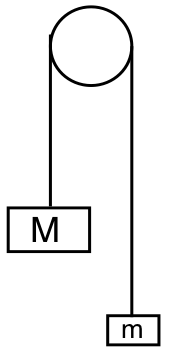
\includegraphics[width=0.1\linewidth]{act223-atwood}
	\end{center}
	
	Based on your intuition which set of attached masses, each differing by \unit[20]{g}, will move faster when released?
	
	\begin{center}
	\begin{tabular}{lll}
		\textbf{Set A:}	&	$M_A = \unit[220]{g}$,	&	$m_A = \unit[200]{g}$\\
		\textbf{Set B:}	&	$M_B = \unit[70]{g}$,	&	$m_B = \unit[50]{g}$
	\end{tabular}
	\end{center}
	\begin{center}
		\begin{tabular}{ll}
		\textbf{Circle your choice here:}	&	(a) Set A moves faster\\
								&	(b) Set B moves faster\\
								&	(c) Both move with the same speed
	\end{tabular}
	\end{center}	
	
	
	\bitem{Put your group's choice on the board.}
	
	How sure are you about your reason(s) and predictions? What is your intuition based on?
	
	\bitem{Try it out}

	Pair up with an adjacent table.  One table will attach the heavier set of masses, the other table should attach the lighter set. Try it out and see which set moves faster. 
	
	What do you observe?

\WCD
\end{benumerate}

\subsection{Applying the \EnergyInteractionModel{}}
\label{act2.2.3-2}

Apply the \EnergyInteractionModel{} to the two-masses-over-a-pulley situation. Model this system as if the pulley is massless and frictionless, so you won't have to worry about energy systems associated with the pulley.\\

\noindent Take the \textbf{initial state} to be just as you release the masses (what is $v_i$? what is $\Delta v$?).\\

\noindent Take the \textbf{final state} to be when the masses have moved a distance $d$ and have speed $v$, but before they hit anything or run out of string.\footnote{Since $d$ denotes a distance, it is a positive number; so, $\Delta y = \pm d$, as appropriate.}

\begin{enumerate}
	\item Create a particular model of the phenomenon described above by constructing a complete \EnergyDiagram{} for \textbf{each} of the mass sets using the initial and final states described above.
	\item	\label{act2.2.3-(2)} When you substitute algebraic expressions for changes in individual energy systems in the algebraic representations of your particular \EnergyInteractionModels{}, you will find the symbols $m$, $M$, $g$, $v$, and $d$ useful. Watch your ``minus signs!''
	\item One important practical use of the \EnergyDiagram{} is in the interpretation of algebraic expressing of energy conservation. For example, what do each of the terms in the equation mean, and what should their sign be? Check, and be ready to show, that the signs of the terms in the equation from \eqref{act2.2.3-(2)} are consistent with the increases and decreases in energy of the energy systems in your diagram.
	\item\label{act2.2.3-(4)} What energy systems have you ignored by your assumptions about the pulley?
	
	[You don't have to put \eqref{act2.2.3-(4)} on the board.]
	
\WCD  
\end{enumerate}
 
\subsection{Reasoning and Explaining with Particular Models}
\label{act2.2.3-3}

You have constructed two particular \EnergyInteractionModels{}, one for each of the different sets of masses. You are now going to use these models to make sense of and explain why one set of the masses (the set with the smaller masses) moved faster than the other set.

\todo[inline]{Should the ``\EnergyInteractionModels{}'' here be ``\EnergyDiagrams{}''? The same goes for any uses of the word ``model.''}

\subsubsection*{Comparing the changes in energy of the various energy systems}

\begin{enumerate}
	\item During the process (from beginning to end), does the total $KE$ of the two masses (the sum of the $KE$s) increase, decrease, or stay the same? How do you know?  Is your response the same for both the heavier and the lighter pair of masses?
	\label{act2.2.3-(5)}
	
	\item During the process, does the total $PE$ of both masses (sum of the $PE$s) increase, decrease, or stay the same? How do you know?  Is your response the same for both the heavier and the lighter pair of masses?
	
	\item Compare the magnitudes of the total change in $PE$ of both masses that occurs during the process across the two systems (the heavier pair and the lighter pair).  Are the total changes the same or different?  Explain.
	
	\item Compare the magnitudes of the total change in $KE$ of both masses that occurs during the process across the two systems (the heavier pair and the lighter pair).  Are the total changes the same or different?  Explain.
	
	\item Did the original question regarding the two sets of masses have to do with the $KE$ of the masses or something else?  Was it related to the $KE$?  Compare this across the two systems (the heavy pair and the lighter pair).  Is this the same or different?  Explain.
	\label{act2.2.3-(9)}
\end{enumerate}

\subsection{Creating a Convincing Scientific Explanation}
\label{act2.2.3-4}

Turn your responses to the questions \eqref{act2.2.3-(5)} through \eqref{act2.2.3-(9)} from \ref{act2.2.3-3} into a set of statements that constitute a logical argument based on your particular \EnergyInteractionModels{} that explains why the set of masses with smaller total mass move faster than the set with greater total mass, as long as the difference between the two masses in each set is the same.\\

\WCD


%%%%%%%%%%%%%%%%%%%%%%%%%%%%%%%%%%%%%%%%%%%%%%%%%%%%%%%%%%%%%%%%%%%%%%%%
%
%		DLM 8
%
%%%%%%%%%%%%%%%%%%%%%%%%%%%%%%%%%%%%%%%%%%%%%%%%%%%%%%%%%%%%%%%%%%%%%%%%

\chapter[\chaptername\thechapter]{\chapterlongname \thechapter}
\label{dlm8}
\addchapter

	\section[More Modeling of Mechanical Energy Systems]{Practicing Graphical and Quantitative Modeling of Mechanical Energy Systems}
%\section{Follow-up of Module 2.2-2.3 FNTs}
\label{act2.3.2}

\begin{overview}

\textbf{Overview:} Before we introduce a new class of physical phenomena, \textbf{\emph{forces}}, we want to make sure you get a bit more practice modeling phenomena using the tools we have accumulated until now, especially the method of graphing energy amounts introduced in the last activities and the carefully crafted model-based, scientific arguments we've been practicing for a while.
	
\end{overview}

\subsection*{We've done a practice activity like this before:}

At home, please work through all the FNTs listed in this activity. In class, each group will work on a portion of these FNTs to come to a consensus before we discuss the scenarios with the whole class.\\

\begin{fnt}
	\label{fnt2.2.3-1}

This FNT is excellent practice in constructing a scientific argument based on logic that follows directly from the physical situation and the relationships of the models you use to, well, model the situation. This is what science is all about!\\

\noindent Please refer back to \hyperref[act2.2.3]{Activity~\ref*{act2.2.3}}:

\begin{enumerate}[(a)]
	\item Finish any of the prompts from \ref{act2.2.3-2} and \ref{act2.2.3-3} that you were unable to finish during the last discussion lab.
	\label{fnt2.2.3-1a}
	
	\item  Respond to the prompt in \ref{act2.2.3-4}, which asks you to turn your responses to prompts from \ref{act2.2.3-2} and \ref{act2.2.3-3} into a set of statements that constitute a logical argument based on the \EnergyInteractionModel{}.
	
		With your argument, explain why the set of masses with smaller total mass moves faster than the set with greater total mass as long as the difference between the two masses in each set is the same.
	\label{fnt2.2.3-1b}
\end{enumerate}
\end{fnt}

\begin{fnt}
	\label{fnt2.2.1-7}

A \unit[0.4]{kg} mass is attached to a spring that can compress as well as stretch (spring constant \unitfrac[50]{N}{m}). The mass and spring are resting on a horizontal tabletop. The mass is pulled, stretching the spring \unit[48]{cm}. When it is released, the system begins to oscillate.

\begin{enumerate}[(a)]
	\item\label{fnt2.2.1-7a} Assuming the transfer of energy to thermal energy systems is negligible, construct a complete \EnergyDiagram{} that could be used to predict the speed of the mass as it passes a point that is a distance of \unit[39]{cm} from its equilibrium point on the other side of the equilibrium position (spring is compressed).
	
		Substitute all known values of constants and variables into the algebraic expression of energy conservation, and identify any unknown(s). Do you have enough information to find the speed of the mass?
	
	\item\label{fnt2.2.1-7b} Now assume that the effects of friction are not negligible. When pulled back and released as before, the mass now reaches its furthest distance from equilibrium at \unit[40]{cm} on the compressed side (before bouncing back again). Construct a complete \EnergyDiagram{} that could be used to determine the amount of energy transferred to thermal systems when going from the initial stretched position to where it first momentarily stops.
	
		\textbf{Proceed as in part a:} Substitute all known values and identify any unknown(s). Can you determine the increase in thermal energy?
\end{enumerate}
\end{fnt}

\begin{fnt}
	\label{fnt2.2.1-8}

\begin{wrapfigure}{R}{.28\textwidth}
	\vspace{-15pt}
  	\centering
	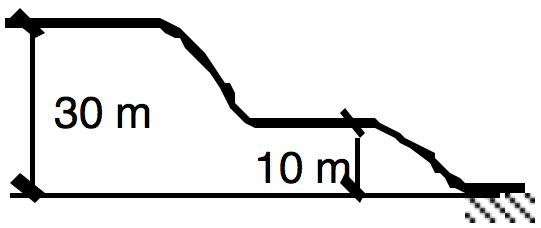
\includegraphics[width=0.95\linewidth]{fnt221-8-hill}
	\vspace{-10pt}
\end{wrapfigure}

A skier (of mass \unit[55]{kg}) skies down the smooth (frictionless) ski slope illustrated in the cross-sectional diagram. She pushes off at the top with a speed of \unitfrac[10]{m}{s}. At the bottom (\unit[0]{m}), she comes to a stop by digging her skis in sideways.

\begin{enumerate}[(a)]
	\item\label{fnt2.2.1-8a} Construct a complete \EnergyDiagram{} that can be used to predict the speed of the skier when she is on the middle flat part (at \unit[10]{m}). Substitute all known values of constants and variables, and identify any unknown(s). Do you have enough information to determine the speed at this part of the hill?

	
	\item\label{fnt2.2.1-8b} Construct a complete \EnergyDiagram{} that can be used to predict the skier's maximum speed just before digging in her skis at the bottom. Substitute for constants and variables and identify any unknown(s) as in Part~\eqref{fnt2.2.1-8a}.

	
	\item\label{fnt2.2.1-8c} Assuming that the snow at the point where she comes to a stop is at a temperature of \unit[0]{\textdegree{}C} and that all of the kinetic energy of the skier goes into melting the snow, construct a complete \EnergyDiagram{} that can be used to predict the amount of snow melted by the skier while stopping. Substitute for constants and variables and identify any unknown(s) as in Part~\eqref{fnt2.2.1-8a}.
\end{enumerate}

\end{fnt}

\begin{fnt}
	\label{fnt2.3.1-1}

\noindent Christine (from \hyperref[act2.2.1b]{Activity~\ref*{act2.2.1b}}) throws a \unit[300]{g} ball straight up into the air. The ball is exactly \unit[2]{m} above the ground when Christine lets go of it. It reaches a height \unit[12]{m} above the height from which it was released, and then falls straight back down.

\begin{enumerate}[(a)]
	\item\label{fnt2.3.1-1a} Assume that $y = 0$ at the point of release of the ball. Find the maximum and minimum values of $y$ and $PE_\text{gravity}$.
	
		What is the total energy of the system? Find the maximum and minimum values of $KE$.

	\item\label{fnt2.3.1-1b} Repeat Part~\eqref{fnt2.3.1-1a}, with $y = 0$ at the ground.	
\end{enumerate}
\end{fnt}

\begin{fnt}
	\label{fnt2.3.1-2}

A \unit[200]{g} mass is attached to a spring, just like in \hyperref[SpringMassActivity]{Activity~\ref{SpringMassActivity}}. The mass is lifted up \unit[5]{cm} and released so that it begins to oscillate about the equilibrium point. The spring has a spring constant $k = \unitfrac[500]{N}{m}$ ($= \unitfrac[500]{J}{m^2}$).

\begin{enumerate}[(a)]
	\item Calculate and accurately plot on a letter size ($\unit[8.5 \times 11]{in}$) sheet of graph paper $PE_\text{spring-mass}$, $E_\text{total}$, and $KE$. The vertical axis of the graph should be energy (in Joules). The horizontal axis is ``distance from equilibrium'' (in Meters). 

	\item On the same graph, quickly sketch (without calculating values) the $PE_\text{spring-mass}$, $KE$ and $E_\text{total}$ of the system if the mass were initially pulled back (stretched) \unit[2.5]{cm} from its equilibrium point, instead of lifted up (compressed) \unit[5]{cm}.
\end{enumerate}
\end{fnt}

\begin{fnt}
	\label{fnt2.3.1-3}

Remember the physical situation described in \ref{fnt2.2.1-8}? To refresh your memory:\\

\begin{wrapfigure}{R}{.28\textwidth}
	\vspace{-15pt}
  	\centering
	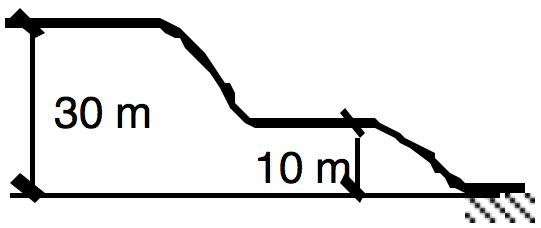
\includegraphics[width=0.95\linewidth]{fnt221-8-hill}
	\vspace{-10pt}
\end{wrapfigure}

\noindent A skier (of mass \unit[55]{kg}) skies down the smooth (frictionless) ski slope illustrated in the cross-sectional diagram. She pushes off at the top with a speed of \unitfrac[10]{m}{s}. At the bottom (\unit[0]{m}), she comes to a stop by digging her skis in sideways.\\

\noindent Use the algebraic expression of energy conservation that shows that the sum of all the energies at all points in time is constant and equal to the total energy for the following:

\begin{enumerate}[(a)]

	\item Pick a location to set $y = 0$ and determine the total energy of the system.
	\item Write an algebraic representation expressing energy conservation that you could use to find the speed of the skier when she is on the middle flat part (at the height \unit[10]{m}).
	\item Substitute all known values of constants and variables, and identify any unknown(s).
	
\end{enumerate}

\end{fnt}

\begin{center}\noindent\textbf{Each group is responsible for putting one of the following on the board.\\ Write so that all other groups can easily follow your presentation!}\end{center}

\noindent\framebox[1.1\width][c]{\textbf{Group 1}}\\

\noindent\ref{fnt2.3.1-1}\\

\noindent For each of Parts~\eqref{fnt2.3.1-1a} and \eqref{fnt2.3.1-1b} of this FNT, make a simple sketch (not a graph) showing the origin 
(where $y = 0$), the ball's initial position, positions $y_\text{max}$ and $y_\text{min}$, and the floor. Then, for each of your two sketches, show how to find the maximum and minimum values of gravitational potential energy, and the total energy.\\

\noindent Be ready to explain how changing the location of where $y = 0$ will affect $PE_\text{gravity}$.\\

\noindent\framebox[1.1\width][c]{\textbf{Group 2}}\\

\noindent\ref{fnt2.3.1-2}

\begin{enumerate}[(a)]
	\item Draw $PE_\text{spring-mass}$ and $E_\text{total}$ (but not $KE$) on a graph of Energy vs.\ ``Distance ($x$) from equilibrium'' for the case of the mass displaced \unit[5]{cm} from equilibrium and released. Clearly label the maximum and minimum values of $PE_\text{spring-mass}$.
	
	\item Demonstrate how to use point by point plotting to graph the $KE$ by doing the following: For at least two different values of $x$, use energy conservation in the form: ``$KE = E_\text{total} - PE$'' to plot a point representing the $KE$. Label the graph clearly showing $PE$, $E_\text{total}$, and $KE$ at each point. In the Whole Class Discussion you can show how to then fill in the $KE$ by sketching a dashed line connecting the points with a smooth curve.
	
	\item On the same graph, quickly draw $PE_\text{spring-mass}$ and $E_{total}$ (but not $KE$) for the case of the mass displaced \unit[2.5]{cm} from equilibrium.
\end{enumerate}

\noindent\framebox[1.1\width][c]{\textbf{Group 3}}\\

\noindent\hyperref[fnt2.2.1-7a]{\ref*{fnt2.2.1-7} Part~\ref*{fnt2.2.1-7a}}\\

\noindent Construct a complete \EnergyDiagram{} with accompanying equations as directed in Part~\eqref{fnt2.2.1-7a} of this FNT, and be ready to explain if you have enough information to determine the speed of the mass.\\

\noindent\hyperref[fnt2.2.1-7b]{\ref*{fnt2.2.1-7} Part~\ref*{fnt2.2.1-7b}}\\

\noindent Construct a complete \EnergyDiagram{} with accompanying equations as directed in Part~\eqref{fnt2.2.1-7b} of this FNT, and be ready to explain if you have enough information to determine the increase in thermal energy.\\
 
\noindent\framebox[1.1\width][c]{\textbf{Group 4}}\\

\noindent\hyperref[fnt2.2.1-8a]{\ref*{fnt2.2.1-8} Part~\ref*{fnt2.2.1-8a}}\\

\noindent Construct a complete \EnergyDiagram{} with accompanying equations as directed in Part~\ref*{fnt2.2.1-8a} of this FNT, and be ready to explain if you have enough information to determine the speed of the skier on the middle part of the hill.\\

\noindent\framebox[1.1\width][c]{\textbf{Group 5}}\\

\noindent\hyperref[fnt2.2.1-8b]{\ref*{fnt2.2.1-8} Part~\ref*{fnt2.2.1-8b}}\\

\noindent Construct a complete \EnergyDiagram{} with accompanying equations as directed in Part~\eqref{fnt2.2.1-8b} of this FNT, and be ready to explain if you have enough information to determine the speed of the skier at the bottom of the hill.\\

\noindent Could you have used different initial values of energy system indicators to answer the same question? Briefly show/explain on the board.\\

\noindent\framebox[1.1\width][c]{\textbf{Group 6}}\\

\noindent\ref{fnt2.3.1-3}\\

\noindent Put your response for this FNT on the board. Be sure to show how you determined the total energy of the physical system.\\

\noindent Is this the only correct value of total energy for the system? Briefly show/explain.\\

\noindent\framebox[1.1\width][c]{\textbf{All Groups}}\\

\noindent\ref{fnt2.2.3-1}\\

\noindent Put your response for this FNT on the board.\\

\WCD
	\newpage
	\section{Connecting Potential Energy with Forces}
\label{act2.4.1}

\begin{overview}

\textbf{Overview:} We have studied two different potential energy systems so far,  $PE_\text{gravity}$ and $PE_\text{mass-spring}$. Our goal in this section is to understand how the forces associated with these potential energy systems are related to the graph of Potential Energy as a function of position.

\end{overview}

\subsection{Graphs for Gravitational Potential Energy}
\label{act2.4.1-1}

\begin{enumerate}
	\item Sketch a graph of $PE_\text{gravity}$ vs.\ the vertical position $y$ of a ball that is thrown upward from the surface of the Earth. Let $y = 0$ be at the ground.
	
		\textbf{Note:} Be sure to plot $PE$ on the vertical axis and $y$ on the horizontal axis.
	
	\item Next to your graph, write a mathematical expression for $PE_\text{gravity}$ as a function of $y$.
	
	\item Consider a particular value of $y$ that is greater than $y_{min}$ and less than $y_{max}$. At your value of $y$, what is the direction of the force of gravity on the ball (in the direction of \emph{decreasing $y$} or \emph{increasing $y$})?
	
		Put an arrow on your graph showing the direction of the force. Repeat for a different value of $y$. How do the magnitudes of the forces at these two points compare?
	
	\item What, in general, can you say about the magnitude and direction of the force at different $y$-values?
\end{enumerate}

\subsection{Graphs for Mass-Spring Potential Energy}
\label{act2.4.1-2}

\begin{enumerate}
	\item Sketch a graph of $PE_\text{mass-spring}$ vs.\ the distance $x$ of a mass from its equilibrium position in an oscillating mass-spring system. Remember that for a mass-spring system, we always set the origin of the coordinate system at the equilibrium point.
	
	\item Next to your graph, write an algebraic expression for $PE_\text{mass-spring}$ as a function of $x$.
	
	\item Consider a particular value of $x$ that is greater than zero and less than $x_{max}$. At your value of $x$, what is the direction of the force on the mass (\emph{away} from equilibrium or \emph{toward} equilibrium), and is that in the direction of \emph{increasing $PE$} or \emph{decreasing $PE$}?
	
		\textbf{Note:} You can use the mass-spring system at your table to test this. Pull the mass down \unit[\about2]{cm} from equilibrium, and then push it up \unit[\about2]{cm} from equilibrium.
		
		Put an arrow on your graph showing the direction of the force. Repeat for a different value of $x$. How do the magnitudes of the forces at the two points compare?
	
	\item What, in general, can you say about the magnitude and direction of the force at different $x$-values?
\end{enumerate}

\subsection{The Big Idea}

\begin{overview}

\textbf{Remember our goal:} We want to relate our observations about the gravitational forces in \ref{act2.4.1-1} and the mass-spring forces in \ref{act2.4.1-2} to features of the graphs of the potential energy systems associated with these forces. That is, we want to find a relationship that \textbf{holds true for both forces}.
	
\end{overview}

\noindent This relationship will need to relate \textbf{both} the \textbf{magnitude} of the force and the \textbf{direction} of the force to \textbf{specific features} of the \textbf{graphs} of the respective potential energies. The two features of the graphs we will focus on are the \textbf{instantaneous slope} of the graph of $PE(y)$ or $PE(x)$, and the \textbf{change in $PE$} as the position changes.

\begin{enumerate}
	\item Can you find any correlation between the magnitude of the force and the magnitude of the instantaneous slope of the $PE$ for these two forces?
	
	\item Can you find any correlation between the direction of the force and the direction of decreasing $PE$ for these two forces?
	
	\item Come to a group consensus about how to state this relationship most succinctly and clearly in words. \textbf{Write this statement on the board.}
\end{enumerate}

\subsubsection*{``Physicality Check''}

When you use the feature you found above to predict a force from the potential energy vs.\ distance graphs, do your results make sense physically?  For example, do the directions and magnitudes of the forces found at various points on the graph agree with what you know about the force?  Try this with various points on both sets of graphs. Be ready to demonstrate this for the whole class.\\

\WCD
	\newpage
	\todo{This badly needs formatting! Skipping for now because this is already printed and it does not seem like we have these FNTs in this version of the manual. Need to look at this before next semester!}

Follow-up of Module 2.4 FNTs

➢	Groups 1 \& 2 discuss and respond to FNT 2.4.1-1 as directed below. 
➢	Groups 3 \& 4 discuss and respond to FNT 2.4.2-1 as directed below. 
➢	Groups 5 \& 6 discuss and respond to FNT 2.4.2-2 as directed below. 

FNT 2.4.1-1 (\unit[\textless10]{min})  
α)	Come to a consensus in your SG about how the changes in $PE_\text{grav}$ compare for the two situations. 
β)	Come to a consensus in your SG about how the maximum heights compare. 

All members of your group must now go to the board and work on this together 

χ)	After you reach consensus (and check with your instructor) about (α) and (β), sketch the two plots of $PE_\text{gravitational}$ on the same graph of Energy vs.\ Height.  
δ)	You know that the force of gravity is constant near the surface of the earth and near the surface of the moon, and that it is approximately six times stronger for the earth than for the moon.  Make sure everyone in your SG is ready to explain how your graph conveys this information.  


All members of your group must now go to the board and work on this together 

FNT 2.4.2-1 (\unit[\textless10]{min})  
α)	For two masses connected by a spring the potential energy is given by: 
$PE_\text{spring} = \frac{1}{2} k(r-r_0)^2$
How does doubling the force constant affect $PE_\text{spring}$ at any particular value of $r$? 
β)	On one graph, sketch two plots of $PE$ for the two different springs. Pick some particular value of $r$, and show explicitly on your graph how doubling the spring constant affects the potential energy of the system. How do these two systems differ physically?
χ)	On a second graph, sketch two plots of $PE$ for the two different values of $r_0$. How do these two systems differ physically?  

All members of your group must now go to the board and work on this together 

FNT 2.4.2-2 (\unit[\textless10]{min})  
α)	Why do we define the $PE$ between atoms or molecules to be zero when $r$ is very large (i.e., when the atoms are far apart instead of when they are close together)? 
β)	Sketch three separate graphs of $PE$ vs.\ separation distance on the board: one for a pair of positively charged particles, one for a pair of negatively charged particles, and one for two particles with opposite charges. Make sure everyone in your SG is ready to explain why the graphs are drawn as they are.


\WCD

	
\part[Forces and Motion: Momentum Conservation]{Forces and Motion:\\The \pModel{}}
\label{Unit6}
	
	%%%%%%%%%%%%%%%%%%%%%%%%%%%%%%%%%%%%%%%%%%%%%%%%%%%%%%%%%%%%%%%%%%%%%%%%
%
%		DLM 9
%
%%%%%%%%%%%%%%%%%%%%%%%%%%%%%%%%%%%%%%%%%%%%%%%%%%%%%%%%%%%%%%%%%%%%%%%%

\mychapter{dlm9}

	\section{Adding and Subtracting Vectors}
\label{act6.1.1}

\begin{overview}

\textbf{Overview:} After studying the energy dynamics of mechanical systems, we're now moving on to take a look at some of the underlying mechanisms and some of the effects of energy transfers and transformations: \textbf{\emph{forces and motion}}. Since we will spend some time and effort on quantitatively describing both, we need to get familiar with mathematical entities that will make this quantitative treatment possible: \textbf{\emph{vectors}}.

\end{overview}

\subsection{Vectors}

Often, a physical quantity cannot be fully described without giving both a magnitude and a direction for it. For instance, consider two physical quantities, mass and force. Suppose I have an object with a mass of \unit[5.0]{kg} and another with a mass of \unit[1.5]{kg}. What is the range of possible values for the total mass of these two objects (i.e. how big might the total mass be and how small might it be)?

Now suppose I push on some object with a force of \unit[2.5]{N} and you push on it with a force of \unit[1.5]{N}. What is the range of values for the total force on the object?  Explain. (\textbf{Hint:} the forces might be in the same directions or in opposite directions.)

\WCD

\subsection{Vector Addition}

\begin{enumerate}
	\item
	  % We have to create a parbox here because wrapfigure does not support enumerate environments directly
	  \parbox[t]{\dimexpr\textwidth-\leftmargin}{%
      \vspace{-3.9mm}
      \begin{wrapfigure}[6]{r}{1.5cm}
        \centering
        \vspace{-\baselineskip}
			\begin{tikzpicture}{r}{1cm}
			% draw the first arrow; "Stealth" is the name of the arrowhead, and it's capitalized, so that it's scalable
			\draw[-{Stealth[scale=1]}, line width=0.8pt] (0,0) -- (0,2.25) node[midway, left=3pt]{$\vec{F}_1$};
			% draw the second arrow
			\draw[-{Stealth[scale=1]}, line width=0.8pt] (0.6,0.5) -- (0.6,2) node[midway, right=3pt]{$\vec{F}_2$};
			\end{tikzpicture}
	  \end{wrapfigure}
      The picture to the right shows two force vectors. $\vec{F}_1$ represents a force of \unit[2.5]{N} pushing straight up the page and $\vec{F}_2$ a force of \unit[1.5]{N} pushing straight up the page. Decide in your groups what the magnitude and direction of the total force acting on an object would be if both $\vec{F}_1$ and $\vec{F}_2$ were acting on it at the same time. Then decide how you should arrange the two vectors that are shown to represent the addition of these vectors showing how you get the total vector that you expect.
      }
	
	\textbf{Hint:} You can easily move the vectors around so that either:
	\vspace{-6pt}
	\begin{enumerate}[(i)]
		\item their tails touch, 
		\item their heads touch, or 
		\item the tail of one touches the head of the other.
	\end{enumerate}
	
	Which of these three methods best demonstrates addition of these two vectors to find the proper total vector?  Sketch this method on the board and also sketch the total force (also called the ``net force'' or the ``sum of the forces'', $\vec{F}_\text{net} = \sum \vec{F}$).
		
	\item 
	  % We have to create a parbox here because wrapfigure does not support enumerate environments directly
	  \parbox[t]{\dimexpr\textwidth-\leftmargin}{%
      \vspace{-2.9mm}
      \begin{wrapfigure}[6]{r}{5cm}
        \centering
        \vspace{-\baselineskip}
			\begin{tikzpicture}{r}{3cm}
			% draw the first arrow; "Stealth" is the name of the arrowhead, and it's capitalized, so that it's scalable
			\draw[-{Stealth[scale=1]}, line width=0.8pt] (0,0) -- (0,2.25) node[midway, left=2pt]{$\vec{F}_1$};
			% draw the second arrow
			\draw[{Stealth[scale=1]}-, line width=0.8pt] (0.75,0.5) -- (0.75,2) node[midway, right=2pt]{$\vec{F}_2$};
			% draw the third arrow
			\draw[-{Stealth[scale=1]}, line width=0.8pt] (1.75,1.25) -- (3.25,1.25) node[midway, above=1pt]{$\vec{F}_3$};
			\end{tikzpicture}
	  \end{wrapfigure}
	The picture to the right shows three force vectors. Show that your method from Part~1 gives a sensible result if $\vec{F}_1$ and $\vec{F}_2$ are the two forces acting on an object. Show that your method works if $\vec{F}_1$ and $\vec{F}_3$ are the two forces acting on an object.
	}
\end{enumerate}

\WCD

\subsection{Vector Subtraction}

\begin{enumerate}
	\item
		  % We have to create a parbox here because wrapfigure does not support enumerate environments directly
	  \parbox[t]{\dimexpr\textwidth-\leftmargin}{%
      \vspace{-2.9mm}
      \begin{wrapfigure}[10]{r}{5cm}
        \centering
        \vspace{-\baselineskip}
			\begin{tikzpicture}{r}{3cm}
				% draw the vertical axis
				\draw[-{Stealth[scale=1.2]}, line width=.5pt] (0,-1.5) -- (0,2.5) node[left=2pt]{$y$};
				% draw the horizontal axis
				\draw[-{Stealth[scale=1.2]}, line width=.5pt] (-0.5,0) -- (4,0) node[below=2pt]{$x$};
				
				% draw points and coordinates
				\fill (2,-1) circle[radius=2pt] node[right=1pt]{\scriptsize{$(x_i,y_i)$}}; 
				\fill (3.5,1) circle[radius=2pt] node[right=1pt]{\scriptsize{$(x_f,y_f)$}}; 

				% draw R_i
				\draw[-{Stealth[scale=1]}, line width=1pt] (0,0) -- (2,-1) node[midway, below=2pt]{$\vec{R}_i$};
				% draw R_f
				\draw[-{Stealth[scale=1]}, line width=1pt] (0,0) -- (3.5,1) node[midway, above=2pt]{$\vec{R}_f$};
				
				% draw connecting lines
				\draw[dashed, line width=.1pt] (2,-1) -- (2,0);
				\draw[dashed, line width=.1pt] (2,0.02) -- (3.5,0.02);
				\draw[dashed, line width=.1pt] (3.5,0) -- (3.5,1);
			\end{tikzpicture}
	  \end{wrapfigure}	
	An object starts at the initial location ($x_i$, $y_i$) as shown in the $x$-$y$ graph to the right and then follows the dashed line path shown to a final location ($x_f$,$y_f$). The picture also shows the initial and final position vectors (position is always measured with respect to some axis origin so all position vectors are drawn from the origin to the position of the object). Draw this figure on the board. Then decide in your groups what arrow you would draw to represent the change in the position, $\Delta\vec{R}$ (both the distance moved as well as the direction moved) and then draw this vector on the board.
	
	}
	
	\item Like before, we define the change in a quantity to be the final value minus the initial value: $\Delta\vec{R} = \vec{R}_f - \vec{R}_i$. Decide in your groups whether $\vec{R}_i$ and $\vec{R}_f$ should be arranged tail-to-head, tail-to-tail, etc. to represent the subtraction of these vectors and show how you get the change $\Delta\vec{R}$ that you expected.
	
	(\textbf{Hint:} This might be easier thank you think.)
	
	\item Does the method used above give you a reasonable $\Delta\vec{v}$ for the two velocity vectors shown below?
\end{enumerate} 

\begin{center}
	\begin{tikzpicture}{r}{1cm}
		% draw the first arrow; "Stealth" is the name of the arrowhead, and it's capitalized, so that it's scalable
		\draw[-{Stealth[scale=1]}, line width=0.8pt] (0,0) -- (0,2) node[midway, left=3pt]{$\vec{v}_i$};
		% draw the second arrow
		\draw[{Stealth[scale=1]}-, line width=0.8pt] (0.6,0) -- (0.6,2) node[midway, right=3pt]{$\vec{v}_f$};
	\end{tikzpicture}
\end{center}

\WCD
 

	\newpage
	\section{Working with Position and Displacement Vectors}
\label{act6.1.2}

\begin{overview}

\textbf{Overview:} Now that we know the basic properties of vectors, let's talk about two similar, yet very different kinds of vectors: \textbf{\emph{position}} and \textbf{\emph{displacement vectors}}.

\end{overview}

\noindent\textbf{Phenomenon:} You are in a strange city that has streets that are laid out in a perfectly square grid. Your job will be to move around to different locations as instructed and record your progress.\\

\noindent\textbf{Make sure everyone in your group fully understands the ideas behind each question or part in these activities before going on to the next part.}

\begin{enumerate}
	\item Make a drawing on the board showing the streets in the central city (this should be a square grid with at least 10 streets going in each direction). Decide as a group how you are going to label the streets and use your labeling system. Make sure your diagram is large enough for everyone in the room to clearly see it.

	\item Near one of the edges of the diagram, label a street corner ``o'' for origin of your coordinate system. Your origin should be different from the origins in other groups' drawings. Sketch a coordinate system so that the $y$-axis points North and the $x$-axis points East.
	
	You start walking somewhere in the city, so choose an intersection near the lower middle part of your diagram, and call that location your ``initial'' position. Draw a position vector on your diagram that shows this initial position. Label this vector ``$\vec{R}_i$.''
	
	\begin{enumerate}
		\item Write $\vec{R}_i$, in terms of its $x$- and $y$-components, as $\left(R_{i,x}, R_{i,y}\right)$. Determine the length of $\vec{R}_i$. What units does it have? How would you describe the direction of the position vector?

\WCD
\vspace{12pt}

		\item Starting from your initial location, imagine walking a distance equal to 4~blocks North and then 1~block West and then 1~block South to a ``final'' location. Show the \emph{position vector}, $\vec{R}_f$, for this new location and write $\vec{R}_f$ in terms of its components as $\left(R_{f,x}, R_{f,y}\right)$.
		
		\item As you might expect, we define the ``change in position'' to be $\Delta \vec{R} = \vec{R}_f - \vec{R}_i$, so that $\vec{R}_i + \Delta \vec{R} = \vec{R}_f$.
		
		Using the tail-to-head method shown on Page~38 of the course notes, redraw the vectors $\vec{R}_i$ and $\vec{R}_f$ off to the side of your map. Then show how you can \textbf{graphically obtain} $\Delta \vec{R}$ from $\vec{R}_i$ and $\vec{R}_f$. Make sure you draw these vectors with the same lengths and directions that they have on your map.
		
		Using the same picture that you used to show $\Delta \vec{R} = \vec{R}_f - \vec{R}_i$, show that $\vec{R}_i + \Delta \vec{R} = \vec{R}_f$ is also true. Now transfer your $\Delta \vec{R}$ over to your street diagram.
		
		\item In physics, we are interested in describing motion. If you could choose only one vector from $\vec{R}_i$, $\vec{R}_f$, and $\Delta \vec{R}$ to describe your motion, which one would it be? Why? What do either of the other two vectors, by themselves, tell you about your motion?
		
		\item How are the $x$-components of $\vec{R}_i$ and $\vec{R}_f$ related to the $x$-component of $\Delta \vec{R}$? How about the $y$-components?

\WCD
\vspace{12pt}

		\item Suppose you walked the 4~blocks North and 1~block West and 1~block South in 60~seconds. Draw the \emph{average velocity} vector for this situation. Write this average velocity vector in component form, $\left(v_x , v_y\right)$. What is the ``length'' of this vector? Include the units. Draw another velocity vector for a situation where you took 180~seconds for this 6~block walk. Which arrow is longer? Why?
		
		\item In which direction(s) would your \emph{instantaneous velocity} be?
		
		\item If you now walked back to your initial point and assuming the total journey took eight hours what is your average velocity for the entire trip?
	\end{enumerate}

\WCD
\vspace{12pt}

	\item Look around the room at the different street diagrams. What is similar in each one? What is different? Discuss in your group how you would summarize the meaning of everything you did in this activity. Be prepared to share with the whole class.
\end{enumerate}
 




%%%%%%%%%%%%%%%%%%%%%%%%%%%%%%%%%%%%%%%%%%%%%%%%%%%%%%%%%%%%%%%%%%%%%%%%
%
%		DLM 10A
%
%%%%%%%%%%%%%%%%%%%%%%%%%%%%%%%%%%%%%%%%%%%%%%%%%%%%%%%%%%%%%%%%%%%%%%%%

\mychapter{dlm10a}

	\section{Check for Understanding: Vector Operations}

\begin{overview}

\textbf{Overview:} In this section, we'll apply our newly-gained knowledge about vectors.

\end{overview}

\label{act6.1.3}

\begin{fnt}
	\label{fnt6.1.2-1}Three force vectors are added together. One has a magnitude of \unit[9]{N}, the second one a magnitude of \unit[18]{N}, and the third a magnitude of \unit[15]{N}. What can we conclude about the magnitude of the net force vector?  Explain.

\begin{enumerate}[I.]
	\item It must equal \unit[42]{N}.
	
	\item It cannot be \unit[0]{N}.
	
	\item Anything from \unit[-42]{N} to \unit[+42]{N}.
	
	\item It can be anything from \unit[0]{N} to \unit[42]{N}.
	
	\item None of the above can be concluded.
\end{enumerate}
\end{fnt}

\vspace{-10pt}
\WCD
\vspace{3pt}

\begin{fnt}
	\label{fnt6.1.2-2}

Alice, Bob and Chuck are three friends standing around, talking. We know that Alice is standing \unit[9]{m} away from Bob, and that Bob is standing \unit[3]{m} away from Chuck. Let $\Delta \vec{R}_\text{AB}$ be the vector that starts at Alice and ends at Bob, and $\Delta \vec{R}_\text{BC}$ be the vector that starts at Bob and ends at Chuck.

\begin{enumerate}[(a)]
	\item Write an equation to find the displacement between Alice and Chuck.
	
	\item What is the furthest distance Chuck can be from Alice, given the information in the question? What is the closest they can be?
	
	\item Draw a picture where Chuck is neither as close as he can be or as far as he can be from Alice. Draw and label the vectors $\Delta \vec{R}_\text{AB}$ and $\Delta \vec{R}_\text{BC}$. 
\end{enumerate}
\end{fnt}

\vspace{-10pt}
\WCD

\begin{fnt}
	\label{fnt6.1.2-3}

\begin{wrapfigure}{R}{0.5\textwidth}
	\vspace{-20pt}
	\begin{center}
	\begin{tikzpicture}[thick,scale=0.65, every node/.style={transform shape},background rectangle/.style={fill=white}, show background rectangle]
		% draw a 10x7.5 grid in light gray with 5mm grid spacing
		\draw[step=.5cm,gray,very thin] (0,0) grid (10,7.5);
		% draw a darker grid in light gray with 2.5mm grid spacing
		\draw[step=2.5cm,gray,thick] (0,0) grid (10,7.5);
    
		% draw the first arrow; "Stealth" is the name of the arrowhead, and it's capitalized, so that it's scalable
		\draw[-{Stealth[scale=1.2]}, line width=1.5pt] (0.5,7) -- (2.5,5);
		% draw label A on top of the first vector
		\draw (2.5,5) node[above=12pt,align=center] {$\vec{A}$};
    
		% draw the second arrow, with descriptor B
		\draw[-{Stealth[scale=1.2]}, line width=1.5pt] (8.5,7) -- (8.5,3) node[right=3pt]{$\vec{B}$};
    
		% draw the second arrow, with descriptor C
		\draw[-{Stealth[scale=1.2]}, line width=1.5pt] (7.5,1) -- (2,1) node[above=3pt]{$\vec{C}$};

	\end{tikzpicture}
	\end{center}
	\vspace{-10pt}
\end{wrapfigure}

\noindent Using a piece of graph paper, carry out the operations listed below on the vectors shown at right. Label all vectors.

\begin{enumerate}[(a)]
	\item $\vec{A}$ + $\vec{B}$
	\item $\vec{B}$ + $\vec{A}$
	\item $\vec{A}$ - $\vec{B}$
	\item $\vec{A}$ + $\vec{B}$ + $\vec{C}$
	\item $\vec{B}$ - $\vec{A}$
	\item -$\vec{C}$
\end{enumerate}
\end{fnt}

\vspace{-10pt}
\WCD
\vspace{3pt}

\begin{fnt}
	\label{fnt6.1.2-4}

\begin{wrapfigure}{R}{0.5\textwidth}
	\vspace{-35pt}
	\begin{center}
	\begin{tikzpicture}[thick,scale=0.65, every node/.style={transform shape},background rectangle/.style={fill=white}, show background rectangle]
		% draw a 10x7.5 grid in light gray with 5mm grid spacing
		\draw[step=.5cm,gray,very thin] (0,0) grid (10,7.5);
		% draw a darker grid in light gray with 2.5mm grid spacing
		\draw[step=2.5cm,gray,thick] (0,0) grid (10,7.5);
    
		% draw the first arrow; "Stealth" is the name of the arrowhead, and it's capitalized, so that it's scalable
		\draw[-{Stealth[scale=1.2]}, line width=1.5pt] (6,5.5) -- (2,5.5);
    
		% draw the vector equation on top of the first vector
		\draw (4,5.5) node[above=6pt,align=center] {$\Sigma \vec{F} = \vec{F_1} + \vec{F_2} + \vec{F_3}$};
    
		% draw object node
		\draw (5,1) node[circle,minimum size=6pt,fill,inner sep=1pt]{} node[below=3pt]{object};
    
		% draw the second arrow, with descriptor F1
		\draw[-{Stealth[scale=1.2]}, line width=1.5pt] (5,1) -- (3,2) node[above=3pt]{$\vec{F_1}_\text{ on object}$};
    
		% draw the second arrow, with descriptor F2
		\draw[-{Stealth[scale=1.2]}, line width=1.5pt] (5,1) -- (9,5) node[above=3pt]{$\vec{F_2}_\text{ on object}$};

	\end{tikzpicture}
	\end{center}
	\vspace{-10pt}
\end{wrapfigure}

%\begin{wrapfigure}{R}{0.5\textwidth}
%	\vspace{-35pt}
 % 	\centering
%	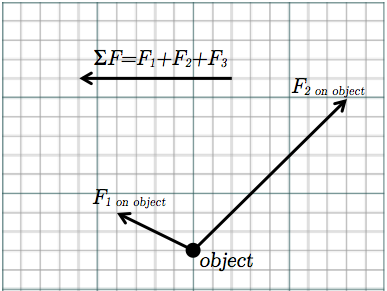
\includegraphics[height=150pt]{fnt612-4-vectors}
%	\vspace{-10pt}
%\end{wrapfigure}

\noindent Vectors $\vec{F}_\text{1 on object}$, $\vec{F}_\text{2 on object}$, and $\vec{F}_\text{3 on object}$ are all exerted on an object, adding together to form a net force vector, $\Sigma \vec{F}$, as shown in the graph to the right. However, only vectors $\vec{F}_\text{1 on object}$, $\vec{F}_\text{2 on object}$, and $\Sigma \vec{F}$ are known.\\

\noindent On a separate piece of graph paper, use the properties of vector addition to graphically determine the vector $\vec{F}_\text{3 on object}$.
\end{fnt}

\vspace{-10pt}
\WCD
	\newpage
	\section[Representing the Motion of a Mass along a Circle]{Using Vectors to Represent the Motion of a Mass Moving in a Circle}
\label{act6.1.4}

\begin{overview}

\textbf{Overview:} So far, we've only talked about linear motion -- an object moving along a straight path. However, many phenomena have objects moving along curved paths. As an example, we'll take a closer look at an object moving along a circle.

\end{overview}

\noindent\textbf{Phenomenon:} You are going to swing a ball in a circle and represent its velocity in several different ways using vectors.\\

\noindent\textbf{Make sure everyone in your group fully understands the ideas behind each question or part in these activities before going on to the next part.}


\begin{enumerate}
	\item \begin{enumerate}
		\item Get the ball swinging in a \emph{large} horizontal \emph{circle}, going \emph{clockwise} when viewed from above:
	\begin{center}
		\begin{tikzpicture}[decoration={markings,mark=at position 0.5*\pgfdecoratedpathlength-25pt with {\arrow[thick]{<}},mark=at position 0.5*\pgfdecoratedpathlength+5.5cm+5pt with {\arrow[thick]{<}}}]
			\node[inner sep=0pt] (fingers) at (-.5,3) {
\includegraphics[width=1cm]{pinchedFingers.png}};
			\draw[postaction={decorate},dashed] (0,0) ellipse (3cm and .8cm);
			\draw (-.18,2.82) -- (1.95,.65);
			\draw[fill=gray] (2,.6) circle (.1);
		\end{tikzpicture}
	\end{center}	
		Imagine looking down on the ball. Pick a position in space that you will identify as the ``12~o'clock'' position. Draw the circular path of the ball on the board with the 12~o'clock position toward the top of the board.
		
		Choose a coordinate system and sketch it on the board.
		
		\item Draw a position vector identifying the position of the ball when it is in the 4~o'clock position. Show the $x$- and $y$-components of this vector on your diagram. Discuss in your group how to do this. Be prepared to share with the whole class.
		
		\item Draw another position vector when the ball is in the 5~o'clock position. To the side of your diagram, graphically subtract the position vectors \textbf{as accurately as possible} to find the displacement vector; label it $\Delta \vec{r}$.
		
		\textbf{\emph{Describe in a sentence what the delta means here.}}
	\end{enumerate}

\vspace{6pt}
\hspace{-\textwidth}\hspace{\linewidth} \textbf{Brief}
\hspace{\textwidth}\hspace{-\linewidth}
\WCD
	
	\item \begin{enumerate}
		\item Describe in words the \textbf{velocity} of the ball as it moves in its circle. Be prepared to share.
		
		\item What do you think is an \emph{instantaneous velocity vector}?  How might it be different from a position vector?  Does it always point in the same direction? If you are having trouble answering these questions, apply them to a specific situation (e.g. driving northwest on I-5 at \unit[65]{mph} and then curving toward the north).
	\end{enumerate}
	
	\item \begin{enumerate}
		\item Imagine that you are sitting on the ball and ``driving'' it in a circle. Which way are you moving when you are at the 4~o'clock position?  Draw a velocity vector (put the tail of the vector at the ball's location) showing the velocity of the ball at the 4~o'clock position. Show the $x$- and $y$-components of this velocity vector on your diagram. Discuss in your group how you do this.
		
		\item  Looking at the vectors you have drawn, is a \emph{position} vector or a \emph{displacement} vector more closely related to a velocity vector? Make sure this agrees with your knowledge of the definition of velocity.
		
		\item Which vectors on your diagram would be different if you changed the origin?
	\end{enumerate}
	
\WCD
	
	\item Draw the velocity vector for the ball at the 6~o'clock position. Off to the side, graphically determine the change in velocity, $\Delta \vec{v}$, between the 4~o'clock position and the 6~o'clock position.
	
	\item \begin{enumerate}
		\item Find the $x$- and $y$-components of the 6~o'clock velocity vector.
		
		\item Find the $x$- and $y$-components of the vector $\Delta \vec{v}$.
		
	\end{enumerate}
	
	\item How can you use the $x$- and $y$-components of the 4~o'clock and the 6~o'clock positions to get the change in velocity, $\Delta \vec{v}$~?  Summarize your method and be prepared to share it with the class.
\end{enumerate}

\WCD
	\newpage


%%%%%%%%%%%%%%%%%%%%%%%%%%%%%%%%%%%%%%%%%%%%%%%%%%%%%%%%%%%%%%%%%%%%%%%%
%
%		DLM 10B
%
%%%%%%%%%%%%%%%%%%%%%%%%%%%%%%%%%%%%%%%%%%%%%%%%%%%%%%%%%%%%%%%%%%%%%%%%

\mychapter{dlm10b}

	\section[Force Model: Net Force and Force Diagrams]{Force Model: Net Force and Force Diagrams\protect{\footnote{See Pages~41-51 of course notes and Force Model Summary.}}}
\label{act6.2.1}

\begin{overview}

\textbf{Overview:} Now that we can represent linear and curved motion with vectors, let's see how vectors are tremendously useful to describe \emph{forces}, as well.

\end{overview}

\noindent\textbf{Phenomenon:} You are going to pull on a metal ring with three ropes attached. A spring is attached to each rope to determine the tension in the rope.

\begin{itemize}
	\item Before you start, make sure each scale is set to zero by twisting the knob.
	\item Work together as a group. No, really: This takes multiple hands!
	\item Attach the ropes with the scales turned so you can read force values in Newtons.
\end{itemize}

\noindent\textbf{Note:} To get the angles to be 130\textdegree{}, trace the ring on a sheet of paper and draw a vertical line pointing down from it. Use a protractor to mark the 130\textdegree{} angles from the vertical line. Line up the ropes along the lines you drew, pull and then note the force scale readings.

\begin{figure}[h!]
	\vspace{-4pt}
	\centering
	\begin{subfigure}[b]{0.45\textwidth}
		\centering
		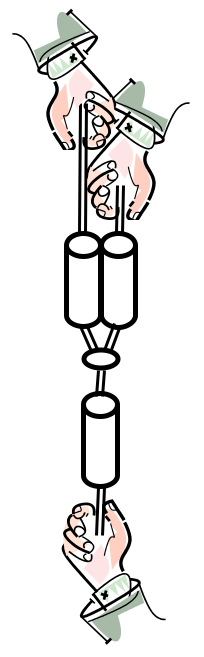
\includegraphics[width=0.25\textwidth]{act621-scenario1}
		\begin{tikzpicture}[thick,scale=0.65, every node/.style={transform shape},background rectangle/.style={fill=white}, show background rectangle]
			% draw object node
			\draw (0,3.5) node[circle,minimum size=12pt,fill,inner sep=1pt]{} node[right=6pt]{Ring};	
			
			% draw and label F1
			\draw[-{Stealth[scale=1.2]}, line width=1pt] (0,3.5) -- (0,5.25) node[right=3pt,align=center] {$\vec{F}_\text{Scale 1 on Ring}$};
			% draw and label F2
			\draw[-{Stealth[scale=1.2]}, line width=1pt] (0,5.25) -- (0,7) node[right=3pt,align=center] {$\vec{F}_\text{Scale 2 on Ring}$};
			
			% draw and label F3
			\draw[-{Stealth[scale=1.2]}, line width=1pt] (0,3.5) -- (0,0) node[right=3pt,align=center] {$\vec{F}_\text{Scale 3 on Ring}$};
		\end{tikzpicture}
		\caption*{\textbf{Scenario 1:} Person~1 and Person~2 pull directly opposite to Person~3 so that the yellow spring scale for the third person reads \unit[30]{N}. Record the values on all three scales.}
	\end{subfigure}
	\hspace{0.05\textwidth}
	\begin{subfigure}[b]{0.45\textwidth}
		\centering
		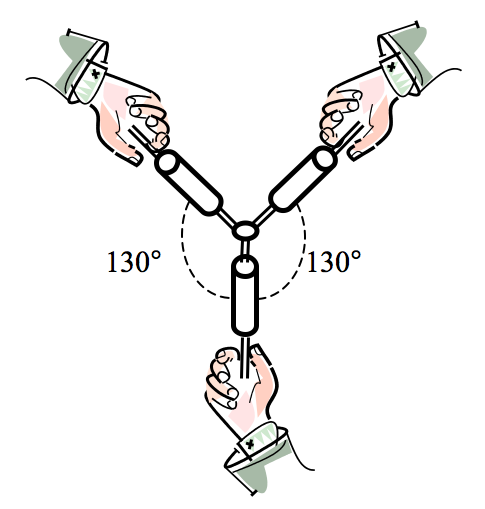
\includegraphics[width=0.5\textwidth]{act621-scenario2}
		\caption*{\textbf{Scenario 2:}  Persons~1 and 2 change the direction they are pulling until their ropes make an angle of about 130\textdegree{} with respect to Person~3. Record the readings of all scales.}
	\end{subfigure}
\end{figure}

\begin{enumerate}
	\item Use appropriately scaled force vectors from the sheet of paper you've used as a guide, and graphically add the three vectors while preserving their angles on the board. What do you get? Why is that? Draw and label all vector components on your graph.
	
	\item A properly labeled and scaled force diagram for the ring is shown for Scenario 1 (on the left, above). \textbf{Note:} Two forces acting on the same object and going in the same direction can be drawn as shown here, or both arrows can have their tails attached to the dot.
	
	Draw a properly labeled and scaled force diagrams for the ring as the object that the three forces act on in Scenario 2. Be sure to use the labeling conventions spelled out on Page~43 of the textbook on any force diagram you make.
	
	\item On the board, off to the side of each force diagram, repeat the method of vector addition from (1). What is the net force on the ring in each case? Check: Why does the resultant net force make sense?

\vspace{12pt}
\hspace{-\textwidth}\hspace{\linewidth} \textbf{Brief}
\hspace{\textwidth}\hspace{-\linewidth}
\WCD
	
	\item Use trigonometry (sine and cosine, as appropriate) to find the magnitude of the components ($x$ and $y$) of the two forces, $\vec{F}_\text{Scale 1 on ring}$ and $\vec{F}_\text{Scale 2 on Ring}$. Put responses to the following on the board:
	\begin{enumerate}
		\item What is the relationship between the components of these two forces and the components of the third force?
		
		\item Develop an explanation for this relationship in your small group and be ready to share.
		
		\item Explain why the scale readings changed when the two people pulling parallel separated to form 130\textdegree{} angles with the third force scale.
	\end{enumerate}
\end{enumerate}

\WCD
\vspace{12pt}

\noindent \textbf{Follow-up Question:} Could two people pull their ropes all the way to 180\textdegree{} apart with the third person still pulling at \unit[30]{N}? Include a force diagram in your response. \textbf{Hint:} Think about the components.
 
\vspace{12pt}
\WCD

	\newpage
	\section[Check for understanding: More Vectors]{Check for understanding: Force, Velocity, and Momentum Vectors}
\label{act6.1.3b}

\begin{overview}

\textbf{Overview:} In this section, we'll practice what we've learned about force and velocity vectors, so far.

\end{overview}

\begin{fnt}
	\label{fnt6.1.2-5}

%\missingfigure{Needs a grid showing F1 and F2.}

\begin{wrapfigure}{R}{0.5\textwidth}
	\vspace{-32pt}
	\begin{center}
	\begin{tikzpicture}[thick,scale=0.65, every node/.style={transform shape},background rectangle/.style={fill=white}, show background rectangle]
		% draw a 10x7.5 grid in light gray with 5mm grid spacing
		\draw[step=.5cm,gray,very thin] (0,0) grid (10,7.5);
		% draw a darker grid in light gray with 2.5mm grid spacing
		\draw[step=2.5cm,gray,thick] (0,0) grid (10,7.5);
    
		% draw object node
		\draw (8.5,2.5) node[circle,minimum size=12pt,fill,inner sep=1pt]{} node[below=3pt]{object};
    
		% draw the first arrow, with descriptor F1; "Stealth" is the name of the arrowhead, and it's capitalized, so that it's scalable
		\draw[-{Stealth[scale=1.2]}, line width=1.5pt] (8.5,2.5) -- (6.5,4.5) node[above=6pt,align=center] {$\vec{F}_\text{1 on object}$};
    
		% draw the second arrow, with descriptor B
		\draw[-{Stealth[scale=1.2]}, line width=1.5pt] (8.5,2.5) -- (1.5,2.5) node[above=6pt]{$\vec{F}_\text{2 on object}$};
		
		% label "no net force" and forces to find
		\draw (2,5) node[above=3pt, align=left]{$\Sigma \vec{F} = 0$
								\\$\vec{F}_\text{3 on object}=?$
								\\$\vec{F}_\text{4 on object}=?$};
	\end{tikzpicture}
	\end{center}
	\vspace{-12pt}
\end{wrapfigure}

\noindent Vectors $\vec{F}_\text{1 on object}$, $\vec{F}_\text{2 on object}$, $\vec{F}_\text{3 on object}$, and $\vec{F}_\text{4 on object}$ are all exerted on an object, adding together to form a net force vector $\Sigma \vec{F} = 0$, as shown to the right.

However, only vectors $\vec{F}_\text{1 on object}$, $\vec{F}_\text{2 on object}$, and  $\Sigma \vec{F}$ (which is zero) are known. It is known that $\vec{F}_\text{3 on object}$ is completely vertical, and $\vec{F}_\text{4 on object}$ is completely horizontal.\\

\noindent On a separate piece of graph paper, use the properties of vector addition to determine the magnitudes of the vertical vector $\vec{F}_\text{3 on object}$, and the horizontal vector $\vec{F}_\text{4 on object}$.
\end{fnt}

\WCD
\vspace{12pt}

\begin{fnt}
	\label{fnt6.1.2-6}

%\missingfigure{Needs xy-axes showing F1 and F2}

\begin{wrapfigure}{R}{0.25\textwidth}
	\vspace{-39.5pt}
  	\centering
	\begin{center}
	\begin{tikzpicture}[thick,scale=0.65, every node/.style={transform shape},background rectangle/.style={fill=white}, show background rectangle]
		% draw xy-axes
		\draw[-{Stealth[scale=1.2]}, line width=0.5pt] (0,-0.5) -- (0,5) node[left=6pt,align=center] {$y$};
		\draw[-{Stealth[scale=1.2]}, line width=0.5pt] (-0.5,0) -- (3,0) node[below=6pt,align=center] {$x$};
		
		% draw F1
		\draw[-{Stealth[scale=1.2]}, line width=1.5pt] (0,0) -- (1.15,0.67) node[above=3pt,align=center] {$\vec{F}_1$};
		% Label F1 = 5N
		\node[label={[rotate=30]above:\unit[5]{N}}] at (0.577,0.333) {};
		% draw F1 arc
		\draw[line width=0.5] (0.6,0) arc (0:30:0.6);
		% label F1 arc 30deg
		\node[label={above:30\textdegree}] at (1.25,-0.25) {};
		
		% draw F2
		\draw[-{Stealth[scale=1.2]}, line width=1.5pt] (0,0) -- (0,4) node[right=6pt,align=center] {$\vec{F}_2$};
		% label F2
		\node[label={[rotate=90]left:\unit[15]{N}}] at (-0.125,2.5) {};
		
		% draw and label v_i
		\draw[->] (1.5,3) -- (2.5,3);
		\node[label={center:$\vec{v}_i=\unitfrac[3]{m}{s}$}] at (2,2.5) {};
	\end{tikzpicture}
	\end{center}
\end{wrapfigure}

\noindent Two force vectors ($\vec{F}_1$ and $\vec{F}_2$, as shown to the right) act on a \unit[2]{kg} object that has an initial velocity $\vec{v}_i$ of \unitfrac[3]{m}{s} in the $+x$-direction.

\begin{enumerate}[(a)]
	\item Use trigonometry to find the $x$- and $y$-components of the net force.
	\item Find the magnitude and direction of the net force.
\end{enumerate}
\end{fnt}

\WCD
\vspace{12pt}
\newpage

\begin{fnt}
	\label{fnt6.1.2-7}

Two rolling carts are moving toward each other at the \textbf{same speed}.  Cart 1 has a mass $m_1 = \unit[200]{g}$ and Cart 2 has a mass $m_2 = \unit[400]{g}$.

\begin{enumerate}[(a)]
	\item Draw a velocity vector $\vec{v}$ for each cart.
	
	\item Momentum $\vec{p}$ is a vector defined as $\vec{p} = m\vec{v}$.  Draw a momentum vector for each cart.
	
	\item Add the two momentum vectors together to find the total momentum, $\vec{p}_\text{total} = \vec{p}_1 + \vec{p}_2$.
\end{enumerate}
\end{fnt}

\WCD
\vspace{12pt}

\begin{fnt}
	\label{fnt6.2.1-1}

Rework the parts of Activity \ref{act6.2.1} that you still have questions about. Bring any remaining questions to the next DL meeting.
\end{fnt}

\WCD
	\newpage

	
%\part{Momentum Conservation}
	%%%%%%%%%%%%%%%%%%%%%%%%%%%%%%%%%%%%%%%%%%%%%%%%%%%%%%%%%%%%%%%%%%%%%%%%
%
%		DLM 11
%
%%%%%%%%%%%%%%%%%%%%%%%%%%%%%%%%%%%%%%%%%%%%%%%%%%%%%%%%%%%%%%%%%%%%%%%%

%commentedchapterlabel%\chapter[\chaptername\thechapter]{\chapterlongname \thechapter}
\mychapter{dlm11}

	\section[Momentum and Change in Momentum: 1-D Cases]{Momentum and Change in Momentum:\\One-Dimensional Cases}
\label{act7.1.1}

\todo[inline]{Last semester, we talked about possibly doing "Part C" before "Parts A and B." I rearranged these to do just that. Originally, this first subsection came third.}

\begin{overview}

\textbf{Overview:} We've previously discussed that moving objects have kinetic energy. In this section, we'll see that moving objects have another property, \emph{momentum}. Colloquially, you may be familiar with this property as ``Oomph.''
\end{overview}


\subsection{Getting a Feel for Momentum}
\label{act7.1.1c}

\textbf{Phenomenon:} Collisions of a cart with another object.\\

\noindent In your small group, you are going to observe, talk about, and analyze simple collisions in one dimension using carts that slide almost frictionlessly on a long aluminum track.\\

\noindent\textbf{Please be gentle with the carts and track. Thanks!}\\

\noindent Make sure everyone in your group fully understands the ideas behind each question or part in these activities before going on to the next part.

\begin{enumerate}
	\item Arrange a collision so that a cart sticks to the bumper of the track. Observe the collision several times (observe the motion). Analyze the collision using the \pConsModel{}.
	\begin{enumerate}
		\item Use vectors to represent the various momenta. Draw on the board a \pchart{}. Each column should have appropriately scaled and labeled vectors for either the momentum or the \emph{change} in momentum $\Delta \vec{p}$ during the collision.
		
		\item Write a vector equation for the momentum, off to the side of your chart, with appropriate subscripts on the symbols, to express what you observed during this collision.
		
		\item Describe in words what physically happened (tell a story!) and how conservation of momentum applies in this situation. Draw a force diagram for the cart for the time when its momentum was changing. Put your diagrams, equation, and story on the board, but leave enough space so you can write the responses to (2) for comparison.
	\end{enumerate}
	
	\item Arrange a collision so that a cart bounces off the bumper. Observe the collision several times. Analyze the collision using the \pConsModel{}, and repeat Steps~(a) to (c), as above.
	
	\todo[inline]{We also talked about removing the "elastic/inelastic" language from this and following activities.}
	
%	\item When total kinetic energy is conserved in a collision, we call it an elastic collision. If it is not conserved, we call it an inelastic collision. Classify the two collisions above as elastic or inelastic.
	\item For each of the two collisions above, is the total kinetic energy conserved?
		
%	\item Does an inelastic collision violate conservation of energy?  If not, which other energy systems could the kinetic energy have gone to?
	\item Does a case in which total kinetic energy is not conserved violate the \emph{conservation of energy} law? If not, which other energy systems could the kinetic energy have gone to?
	
%	\item Is momentum conserved in the inelastic case and the elastic case?  Where in your \pchart{} is this shown?
	\item Is momentum conserved in the case where total kinetic energy is conserved and in the case where total kinetic energy is not conserved? Where in your \pchart{} is this shown?
\end{enumerate}

\WCD

\subsection{Change in Momentum and Impulse in One Dimension}
\label{act7.1.1a}

%(See Model Summary \#6)

A change in momentum of an object is caused by a net force acting on the object over a certain amount of time. We define the \emph{Net Impulse} $\Sigma\vec{I}$ as the product of the net force $\Sigma\vec{F}_\text{on object}$ and the amount of time $\Delta t$ during which the net force is acting on the object:
\vspace{-5pt}

\begin{equation*}
	\text{Net Impulse} = \Sigma\vec{I} = \Sigma\vec{F}_\text{on object} \cdot \Delta t
\end{equation*}

\noindent Because a net impulse $\Sigma\vec{I}$ causes a change in momentum $\vec{p}$ of the object, we can also write:
\vspace{-10pt}

\begin{equation*}
	\overset{\mbox{\normalfont\tiny\sffamily cause}}{\text{Net Impulse}} = \Sigma\vec{I} = \Sigma\vec{F}_\text{on object} \cdot \Delta t = \vec{p}_f - \vec{p}_i = \Delta\vec{p} = \overset{\mbox{\normalfont\tiny\sffamily effect}}{\text{Change in Momentum}}
\end{equation*}

\noindent Remember the law of Energy Conservation? We observed that when there is no energy coming into or going out of a given physical system, the total energy of that system is conserved, which means the total change of energy $\sum\Delta E$ is equal to zero. There is a similar phenomenon with momentum, the \emph{Conservation of Momentum}. In this case, the total momentum of a system of objects remains unchanged:
\vspace{-5pt}

\begin{equation*}
	\Delta \vec{p}_\text{system} = \vec{p}_{f,\text{sys}} - \vec{p}_{i,\text{sys}} = 0 \text{  when  } \Sigma\vec{I} = 0 \text{  or  } \Sigma\vec{F} = 0	
\end{equation*}

\begin{enumerate}
	\item In your small group, describe an example of an impulse. Identify two ways you can change this impulse. For instance, how could you make the impulse greater?   Describe both 
	\begin{enumerate}
		\item a system that involves one object and 
		\item a system that involves two interacting objects.
	\end{enumerate}
	Explain what $\Delta \vec{p}_\text{system}$ is for each of your physical systems. Put this on the board.
	
	\item In your small group, develop a statement in your own words of what \textbf{\em conservation of momentum} means for your two systems in (1).
\end{enumerate}

\WCD

\newpage

\section{Representing Momentum Conservation with Vectors}
\label{act7.1.1b}
%(See Page~54 of Course Notes)

\begin{overview}
	\textbf{Overview:} Just as \EnergyDiagrams{} are useful in helping us work through conservation of energy questions/problems, \pcharts{} are useful for questions/problems involving conservation of momentum. The \pchart{}, like an \EnergyDiagram{}, helps us keep track of what we know about the interaction, and it also helps us see what we do not know.
\end{overview}

\noindent\textbf{All \pcharts{} are to be filled in with \emph{scaled} arrows representing momentum vectors.}\footnote{The algebraic expression for a momentum vector is  $\vec{p} = m\vec{v}$, where $\vec{v}$ is the velocity vector. This means that velocity and momentum point in the same direction at any instance in time!}

\begin{figure}[h!]
	\centering
	\begin{subfigure}[b]{0.45\textwidth}
		\centering
		\caption*{\textbf{Closed System}\\Typically used for collisions/interactions involving two or more objects:}
		\begin{tikzpicture}[thin,scale=0.9, every node/.style={transform shape},background rectangle/.style={fill=white}, show background rectangle]
			% draw table
			\draw (0,0) -- (0,4);
			\draw[very thick] (2,0) -- (2,4);
			\draw (4,0) -- (4,4);
			\draw (6,0) -- (6,4);
			\draw (8,0) -- (8,4);
			\draw (0,0) -- (8,0);
			\draw[very thick] (0,1) -- (8,1);
			\draw (0,2) -- (8,2);
			\draw[very thick] (0,3) -- (8,3);
			\draw (0,4) -- (8,4);
			
			% label table
			\node[text width=2cm, align=center] at (1,3.5)
				{Closed $\vec{p}$ system};
			\node[text width=2cm, align=center] at (3,3.5)
				{$\vec{p}_i$};
			\node[text width=2cm, align=center] at (5,3.5)
				{$\Delta\vec{p}$};
			\node[text width=2cm, align=center] at (7,3.5)
				{$\vec{p}_f$};
			\node[text width=2cm, align=center] at (1,2.5)
				{Object 1};
			\node[text width=2cm, align=center] at (1,1.5)
				{Object 2};
			\node[text width=2cm, align=center] at (1,0.5)
				{Total System};
			\node[text width=2cm, align=center] at (5,0.5)
				{0};
		\end{tikzpicture}
		\caption*{For total system: $\Delta \vec{p} = 0$\\
	For each object: $\vec{p}_i + \Delta \vec{p} = \vec{p}_f$}
	\end{subfigure}
	\hspace{0.05\textwidth}
	\begin{subfigure}[b]{0.45\textwidth}
		\centering
		\caption*{\textbf{Open System}\\Typically used when the phenomenon involves a \textbf{net impulse} acting on the system:}
		\begin{tikzpicture}[thin,scale=0.9, every node/.style={transform shape},background rectangle/.style={fill=white}, show background rectangle]
			\draw[white] (0,0) -- (8,0);
			% draw table
			\draw (0,2) -- (0,4);
			\draw[very thick] (2,2) -- (2,4);
			\draw (4,2) -- (4,4);
			\draw (6,2) -- (6,4);
			\draw (8,2) -- (8,4);
			\draw (0,2) -- (8,2);
			\draw[very thick] (0,3) -- (8,3);
			\draw (0,4) -- (8,4);
			
			% label table
			\node[text width=2cm, align=center] at (1,3.5)
				{Open $\vec{p}$ system};
			\node[text width=2cm, align=center] at (3,3.5)
				{$\vec{p}_i$};
			\node[text width=2cm, align=center] at (5,3.5)
				{$\Delta\vec{p}$};
			\node[text width=2cm, align=center] at (7,3.5)
				{$\vec{p}_f$};
			\node[text width=2cm, align=center] at (1,2.5)
				{Total System};
		\end{tikzpicture}
		\caption*{For total system: $\Delta \vec{p} = \Sigma\vec{I}$\\
	\phantom{For total system: } $\vec{p}_i + \Delta\vec{p} = \vec{p}_f$}
	\end{subfigure}
	\caption*{To identify any forces that cause the object's change in momentum (change in motion), it helps to draw a force diagram for each object in the \pchart{}.}
\end{figure}
\vspace{-12pt}

\begin{enumerate}
	\item On your boards, complete the appropriate \pchart{} for each of your examples from Activity~\ref{act7.1.1a}.
	
	\item Each row and each column represent a separate vector equation. Check that every row equation and every column equation are added correctly and are consistent.
	
	\item Which column is significant for showing whether momentum is conserved?
	
	\item Determine what parts of the \pcharts{} are analogous to \EnergyDiagrams{}. List the analogous parts on the board. In what fundamental way do these diagrams differ?
\end{enumerate}

\WCD 


	\newpage
%	\input{U7/act7.1.1c}
%	Review for Midterm
	\section{Check for understanding: 1-D Momentum}
\label{14C.1}

\begin{overview}
	\textbf{Overview:} In this section, we'll practice what we've learned so far about momentum, change in momentum, and momentum conservation.	
\end{overview}

\subsection{Collisions and Other Interactions between Objects}

\begin{fnt}
	\label{fnt7.1.1-1}

You're playing with two of the carts (each with mass $m$) that you used in \hyperref[act7.1.1c]{Activity~\ref*{act7.1.1c}}. Initially, these two carts are moving toward each other with the same initial speed $v_i$ along the track. The carts collide and the result is one of these final states:
\begin{enumerate}[(a)]
	\item Assume that the carts hit each other and stop so that the final state of the system has both carts just sitting still (not moving). Draw a \pchart{} for this situation. Make a separate row for each cart.% Refer to \pConsModel{} 
	\item Assume that the carts bounce off each other so that the final state of the system has each cart moving opposite to its initial motion but with the same speed. Draw a \pchart{} for this situation.
	\label{fnt7.1.1-1b}
	\item As in \eqref{fnt7.1.1-1b}, assume that the carts bounce off each other but now assume that the final speeds are smaller than the initial speeds, equal and in opposite directions. Draw a \pchart{}.
	\item For each case above, does the total momentum of the system that contains the two carts change? How do the \pcharts{} help you answer this question?
	\item Is the total kinetic energy constant for all three cases? How do you know?
\end{enumerate}

\end{fnt}

\begin{fnt}
	\label{fnt7.1.1-2}

A rocket expels gas at a high speed out of its back for a short period of time. We are going to treat the rocket as being far away from any gravitational objects.

\begin{enumerate}[(a)]
	\item Draw a \pchart{} for the rocket expelling gas in space. Take the initial time before expelling gas and the final time after the rocket has finished expelling gas. The rocket has an initial constant speed in the horizontal direction. Put the rocket and the expelled gas on separate rows.
	\item Use your chart to explain why the rocket speed increases. 
	\item Does the rocket have to keep expelling gas to stay at a constant speed? Explain.
\end{enumerate}
\end{fnt}

\begin{fnt}
	\label{fnt7.1.1-3}

Victoria is standing on a boat, during a perfectly calm day. Initially, both Victoria and the boat are not moving. Then Victoria walks from one end of the boat to the other. Take the initial time to be before she walks and the final time at some point while she is still walking.

\begin{enumerate}[(a)]
	\item Draw a \pchart{} for this situation. Does the boat move, and if so, in which direction?
	\item Compare the speed of the boat with Victoria's speed. Are they the same or different? Why?
\end{enumerate}
\end{fnt}

%\subsection*{In Your Small Group}
Compare your responses to \ref{fnt7.1.1-1}, \ref{fnt7.1.1-2}, and \ref{fnt7.1.1-3} with the other members of your small group. Come to a consensus on the appropriate \pcharts{} and answers, and put these on your board.

\textbf{Added problem:} Draw an appropriately scaled force diagram (for each object) that shows all the forces acting during the interaction (when the impulse occurs). Do this for each FNT.

\WCD

\subsection{More Collisions of Two Carts}

\noindent Your instructor will assign each group a situation from 1--3 below and one from 4--5. Use the \pConsModel{} to analyze each of the collisions between two carts in the Situations~1--3 below. You may treat the system made up of the two carts as a closed physical system because there is no net external impulse imparted on the system during the collision.\\

\noindent\textbf{Situations:}
\begin{enumerate}
	\item Use two carts of equal mass, physically arranged so the carts will bounce off one another. Start with \textbf{\em one cart stationary}.
	\item Use two carts of equal mass, physically arranged so the collision ends with the \textbf{\em carts locked (stuck together)}.
	\item Use two carts of equal mass initially \textbf{\em moving toward each other} with equal speed and \textbf{\em ending with the carts locked (stuck together)}.
	\item Place two carts of \textbf{\em unequal mass} on the track, turned so the collision \textbf{\em ends with the carts locked (stuck together)}. Start with one cart stationary, and have the other move to collide with it. Make the stationary cart have more mass. Repeat, switching carts.
	\item Place two carts of \textbf{\em unequal mass} on the track, turned so the collision \textbf{\em ends with the carts locked (stuck together)}. Start with both carts \textbf{\em moving toward each other} with the same speed.
\end{enumerate}

\noindent
\textbf{For each Situation:}
\begin{enumerate}[(a)]
	\item Draw and fill in a \pchart{} to help you describe momentum conservation in this closed physical system.
	\item For each line of the \pchart{}, write an algebraic vector equation, with appropriate subscripts on the symbols, to express what that line tells you about the collision.
	\item Draw a force diagram for each cart that shows the forces \emph{during} the collision.
	\item Describe in words what physically happened and then how conservation of momentum applies to each cart and to the system as a whole. Put your equation and word statement on the board.
	\item Compare the total kinetic energy before the collision to the total kinetic energy after the collision.% Classify each case as elastic or inelastic.
\end{enumerate}

\noindent Observe what is similar and what is different in your \pcharts{}. What patterns can you observe? Discuss in your group any rules you come up with for the patterns.

\WCD %FNTs only


%%%%%%%%%%%%%%%%%%%%%%%%%%%%%%%%%%%%%%%%%%%%%%%%%%%%%%%%%%%%%%%%%%%%%%%%
%
%		DLM 11B
%
%%%%%%%%%%%%%%%%%%%%%%%%%%%%%%%%%%%%%%%%%%%%%%%%%%%%%%%%%%%%%%%%%%%%%%%%

%Commented out because FNTs were incorporated into the previous D/L

%\chapter[\chaptername\thechapter]{\chapterlongname \thechapter}
%\label{dlm11b}
%\addchapter

%	\section{Check for understanding: 1-D Momentum}
\label{14C.1}

\begin{overview}
	\textbf{Overview:} In this section, we'll practice what we've learned so far about momentum, change in momentum, and momentum conservation.	
\end{overview}

\subsection{Collisions and Other Interactions between Objects}

\begin{fnt}
	\label{fnt7.1.1-1}

You're playing with two of the carts (each with mass $m$) that you used in \hyperref[act7.1.1c]{Activity~\ref*{act7.1.1c}}. Initially, these two carts are moving toward each other with the same initial speed $v_i$ along the track. The carts collide and the result is one of these final states:
\begin{enumerate}[(a)]
	\item Assume that the carts hit each other and stop so that the final state of the system has both carts just sitting still (not moving). Draw a \pchart{} for this situation. Make a separate row for each cart.% Refer to \pConsModel{} 
	\item Assume that the carts bounce off each other so that the final state of the system has each cart moving opposite to its initial motion but with the same speed. Draw a \pchart{} for this situation.
	\label{fnt7.1.1-1b}
	\item As in \eqref{fnt7.1.1-1b}, assume that the carts bounce off each other but now assume that the final speeds are smaller than the initial speeds, equal and in opposite directions. Draw a \pchart{}.
	\item For each case above, does the total momentum of the system that contains the two carts change? How do the \pcharts{} help you answer this question?
	\item Is the total kinetic energy constant for all three cases? How do you know?
\end{enumerate}

\end{fnt}

\begin{fnt}
	\label{fnt7.1.1-2}

A rocket expels gas at a high speed out of its back for a short period of time. We are going to treat the rocket as being far away from any gravitational objects.

\begin{enumerate}[(a)]
	\item Draw a \pchart{} for the rocket expelling gas in space. Take the initial time before expelling gas and the final time after the rocket has finished expelling gas. The rocket has an initial constant speed in the horizontal direction. Put the rocket and the expelled gas on separate rows.
	\item Use your chart to explain why the rocket speed increases. 
	\item Does the rocket have to keep expelling gas to stay at a constant speed? Explain.
\end{enumerate}
\end{fnt}

\begin{fnt}
	\label{fnt7.1.1-3}

Victoria is standing on a boat, during a perfectly calm day. Initially, both Victoria and the boat are not moving. Then Victoria walks from one end of the boat to the other. Take the initial time to be before she walks and the final time at some point while she is still walking.

\begin{enumerate}[(a)]
	\item Draw a \pchart{} for this situation. Does the boat move, and if so, in which direction?
	\item Compare the speed of the boat with Victoria's speed. Are they the same or different? Why?
\end{enumerate}
\end{fnt}

%\subsection*{In Your Small Group}
Compare your responses to \ref{fnt7.1.1-1}, \ref{fnt7.1.1-2}, and \ref{fnt7.1.1-3} with the other members of your small group. Come to a consensus on the appropriate \pcharts{} and answers, and put these on your board.

\textbf{Added problem:} Draw an appropriately scaled force diagram (for each object) that shows all the forces acting during the interaction (when the impulse occurs). Do this for each FNT.

\WCD

\subsection{More Collisions of Two Carts}

\noindent Your instructor will assign each group a situation from 1--3 below and one from 4--5. Use the \pConsModel{} to analyze each of the collisions between two carts in the Situations~1--3 below. You may treat the system made up of the two carts as a closed physical system because there is no net external impulse imparted on the system during the collision.\\

\noindent\textbf{Situations:}
\begin{enumerate}
	\item Use two carts of equal mass, physically arranged so the carts will bounce off one another. Start with \textbf{\em one cart stationary}.
	\item Use two carts of equal mass, physically arranged so the collision ends with the \textbf{\em carts locked (stuck together)}.
	\item Use two carts of equal mass initially \textbf{\em moving toward each other} with equal speed and \textbf{\em ending with the carts locked (stuck together)}.
	\item Place two carts of \textbf{\em unequal mass} on the track, turned so the collision \textbf{\em ends with the carts locked (stuck together)}. Start with one cart stationary, and have the other move to collide with it. Make the stationary cart have more mass. Repeat, switching carts.
	\item Place two carts of \textbf{\em unequal mass} on the track, turned so the collision \textbf{\em ends with the carts locked (stuck together)}. Start with both carts \textbf{\em moving toward each other} with the same speed.
\end{enumerate}

\noindent
\textbf{For each Situation:}
\begin{enumerate}[(a)]
	\item Draw and fill in a \pchart{} to help you describe momentum conservation in this closed physical system.
	\item For each line of the \pchart{}, write an algebraic vector equation, with appropriate subscripts on the symbols, to express what that line tells you about the collision.
	\item Draw a force diagram for each cart that shows the forces \emph{during} the collision.
	\item Describe in words what physically happened and then how conservation of momentum applies to each cart and to the system as a whole. Put your equation and word statement on the board.
	\item Compare the total kinetic energy before the collision to the total kinetic energy after the collision.% Classify each case as elastic or inelastic.
\end{enumerate}

\noindent Observe what is similar and what is different in your \pcharts{}. What patterns can you observe? Discuss in your group any rules you come up with for the patterns.

\WCD %FNTs only
%	Review for Midterm


%%%%%%%%%%%%%%%%%%%%%%%%%%%%%%%%%%%%%%%%%%%%%%%%%%%%%%%%%%%%%%%%%%%%%%%%
%
%		DLM 12A
%
%%%%%%%%%%%%%%%%%%%%%%%%%%%%%%%%%%%%%%%%%%%%%%%%%%%%%%%%%%%%%%%%%%%%%%%%

%commentedchapterlabel%\chapter[\chaptername\thechapter]{\chapterlongname \thechapter}
\mychapter{dlm12a}

%	\textbf{Phenomenon:} Collisions of two carts in one dimension, both elastic and inelastic collisions.

Your instructor will assign each group a Situation from 1 -- 3 below and one from 4--5. Use the \pConsModel{} to analyze each of the collisions between two carts in the Situations~1 -- 3 below. You may treat the system made up of the two carts as a closed physical system because there is no net external impulse transferred to the system during the collision.

\noindent
\textbf{Situations:}
\begin{enumerate}
	\item Use two carts of equal mass, physically arranged so the carts will bounce off one another. Start with \textbf{\em one cart stationary}.
	\item Use two carts of equal mass, physically arranged so the collision ends with the \textbf{\em carts locked (stuck together)}.
	\item Use two carts of equal mass initially \textbf{\em moving toward each other} with equal speed and \textbf{\em ending with the carts locked}.
	\item Place two carts of \textbf{\em unequal mass}, on the track turned so the collision \textbf{\em ends with the carts locked}. Start with one cart stationary, and have the other move to collide with it. Make the stationary cart have more mass (repeat, switching carts).
	\item Place two carts of \textbf{\em unequal mass}, on the track turned so the collision \textbf{\em ends with the carts locked}. Start with both carts \textbf{\em moving toward each other} with the same speed.
\end{enumerate}

\noindent
\textbf{For each Situation:}
\begin{enumerate}[(a)]
	\item Draw and fill in a \pchart{} to help you describe momentum conservation in this closed physical system.
	\item For each line of the \pchart{}, write an algebraic vector equation, with appropriate subscripts on the symbols, to express what that line tells you about the collision.
	\item Draw a force diagram for each cart that shows the forces \emph{during} the collision.
	\item Describe in words what physically happened and then how conservation of momentum applies to each cart and to the system as a whole. Put your equation and word statement on the board.
	\item Compare the total kinetic energy before the collision to the total kinetic energy after the collision.% Classify each case as elastic or inelastic.
\end{enumerate}

Observe what is similar and what is different in your \pcharts{}. What patterns can you observe? Discuss in your group any rules you come up with for the patterns.

\WCD %second half
%	\newpage
	\section[The Significance of $\Delta t$]{\protect\boldmath The Significance of $\Delta t$}

\begin{overview}
\textbf{Overview:} The examples and activities in this section illustrate how the time duration $\Delta t$ of an impulse imparted on an object (or system) relates to the net force $\Sigma F$ and the change in momentum of the object (or system) $\Delta \vec{p}$.
\end{overview}

\subsection{The Tablecloth Trick}
\label{act7.1.3B}

\textbf{Phenomenon:} If a tablecloth (or a large piece of paper) is pulled quickly enough from under some objects sitting on it, those objects slide only a very short distance on the table top after the tablecloth has been pulled out from under them. This implies that they acquired only a small velocity from the tablecloth moving out from under them. If the tablecloth is pulled a little less quickly, the objects slide a little further on the table top, implying they acquired a slightly greater velocity.\\

\noindent\textbf{Try the trick:} Use a ``hanging mass'' or another object and a fairly large piece of paper. Try pulling the piece of paper at different rates, so that the object
	\begin{itemize}
		\item moves a lot (but does not fall off the table); and
		\item moves very little.
	\end{itemize}

\noindent In both cases, make sure you are pulling sufficiently fast so that the objects are continually sliding on the paper as it is being pulled. That is, you need to pull sufficiently fast so that the objects do not move with the paper.\\
	
\noindent\textbf{Our goal is to make sense of this phenomenon using the relation of impulse to a force and the time interval over which it acts.}

\subsubsection*{Establishing which part of the phenomenon we need to focus on:}

\begin{enumerate}
	\item The momentum of an object is first increased as the paper is pulled out from under it. Then the momentum is decreased back to zero as it slides to a stop on the table. How far it slides on the table after the paper is pulled out from under it is a qualitative measure of the speed it acquired when the paper was sliding under it: the greater the distance it slid, the greater the speed it had acquired.
	
	So, thinking in terms of impulse and momentum, \textbf{which force} acting through \textbf{what time interval} determined the maximum speed the object acquired before sliding to a stop on the table top?

\vspace{8pt}
\hspace{-\textwidth}\hspace{\linewidth} \textbf{Brief}
\hspace{\textwidth}\hspace{-\linewidth}
\WCD

	Express the friction force, which is the horizontal component of the force the paper exerts on the object, $F_{||\text{ paper on object}}$, as a constant (coefficient of friction $\mu$) times the object's weight $mg$.\footnote{Note that the coefficient will depend on the surfaces of the two materials in contact, but for reasonably smooth surfaces like paper and metal, it generally has a value in the range of 0.5 to 1.0.}
	
	\emph{The important point for the analysis here is that the \textbf{friction force} is \textbf{only proportional to the weight of the object} \boldmath$mg$. It does \emph{not} depend on how fast you pull the paper.}
	
	\item In your small group, make two complete \pcharts{} -- including force diagrams -- for one of the objects on your table (such as keys, small bottles, etc.) that is sitting on a piece of paper, which is pulled out from under it. One \pchart{} should show the process when the paper is pulled quickly, and the second \pchart{} should show the process when it is pulled less quickly. Consider the interval to be just before the pull until immediately after the paper is no longer under the object.
	
	\item Make sure all forces in the force diagrams are appropriately labeled. Does how fast you pull the tablecloth affect the net force acting on the object? Identify exactly what things are exerting forces on your object!
	
	\item Develop an explanation of these phenomena using the \pcharts{} you have prepared. Start by writing out an expression for impulse.
	
	\textbf{Extra question:} Try using different objects for your performance of the tablecloth trick. Do all the objects appear to move about the same distance for a given pull? How can you explain this?
	
	\item If you know the initial and the final momentum, you know the impulse. In each of your scenarios, did you have the same or a different impulse? So what is the effect of changing $\Delta t$? 
\end{enumerate}

\noindent Be prepared to explain what $\Delta t$ is and why it is important in a momentum problem!\\

\noindent Be ready to illustrate and give your explanations to the whole class.

\vspace{8pt}
\WCD
	\newpage
	%\section{The Importance of $\Delta t$ in Collisions}
\subsection{Automobile crash}
\label{act7.1.3A}

%Use the following phenomenon for \ref{fnt7.1.1-4}, \ref{fnt7.1.1-5}, and \ref{fnt7.1.1-6}.\\

\noindent\textbf{Phenomenon:} You are riding in a car that crashes into a solid wall.  The car comes to a complete stop without bouncing back.  The car has a mass of \unit[1500]{kg} and has a speed of \unitfrac[30]{m}{s} before the crash (this is about \unitfrac[65]{mi}{hr}). 

\begin{fnt}
	\label{fnt7.1.1-4}

%You are riding in a car that crashes into a solid wall.  The car comes to a complete stop without bouncing back.  The car has a mass of \unit[1500]{kg} and has a speed of \unitfrac[30]{m}{s} before the crash (this is about \unitfrac[65]{mi}{hr}).  

\begin{enumerate}[(a)]
	\item What is the car's initial momentum?
	\item What is your initial momentum? Recall that the weight of one kilogram is \unit[2.2]{lbs}.
	\item Draw separate \pcharts{} for the car and the person. Treat both as open systems with a net impulse.
	\item What is the change in the momentum of the car?
	\item What is the change in your momentum?
\end{enumerate}
\end{fnt}

\begin{fnt}
	\label{fnt7.1.1-5}

%You are riding in a car that crashes into a solid wall.  The car comes to a complete stop without bouncing back.  The car has a mass of \unit[1500]{kg} and has a speed of \unitfrac[30]{m}{s} before the crash (this is about \unitfrac[65]{mi}{hr}).  

\begin{enumerate}[(a)]
	\item What is the net impulse that acts on the car to bring it to a stop?
	\item What is the net impulse that acts on you to bring you to a stop?
\end{enumerate}
\end{fnt}

\begin{fnt}
	\label{fnt7.1.1-6}

%You are riding in a car that crashes into a solid wall.  The car comes to a complete stop without bouncing back.  The car has a mass of \unit[1500]{kg} and has a speed of \unitfrac[30]{m}{s} before the crash (this is about \unitfrac[65]{mi}{hr}).  

Refer to your \pcharts{} from \ref{fnt7.1.1-4}. Consider the following two situations.

\begin{enumerate}[I.]
	\item You remain buckled into the seat and the seat remains attached to the center of the car.
	\item You are not buckled into your seat and you fly through the windshield and hit the wall.
\end{enumerate}

\begin{enumerate}[(a)]
	\item Is the impulse the same in both cases?
	\item Are the forces acting on you the same?
	\item Using the words impulse, force, time, and momentum explain why one scenario is safer for you.  Hint: Think about how the shape of the car changes when it hits the wall.
\end{enumerate}
\end{fnt}

\begin{enumerate}
	\item In your group, decide on two specific scenarios (\ref{fnt7.1.1-6}) and use these scenarios in Parts~2, 3, and 4 below. For these two scenarios, think about how much time passes between the time the force is first applied by the object and the time when you have zero momentum. In which scenario will this time difference $\Delta t$ be larger and why?
	
	\item  On the board, put up complete \pcharts{} (with force diagrams and equations worked through to numerical values) for the car and for the person in each of the two scenarios you have chosen. Describe the scenario above each of the \pcharts{} for the person.
	
	\item Use your \pcharts{} to explain why the net force acting on the person will not be the same in both scenarios.
	
	\item For each of the scenarios that you described in \ref{fnt7.1.1-6}, estimate the magnitude of the average force that would have been acting on you to bring you to a stop.
	\begin{enumerate}
		\item You will have to determine the time during which the impulse acts for the different scenarios. To do this you must first decide on the initial and final momentum for the cases you are describing and over \emph{what distance} the impulse acts.
		
		\item Now you need to \emph{calculate} the time duration of the impulse using your knowledge of how distance and time are related. If you assume that you slow down at a constant rate, then your average speed during this time is one-half your initial speed.
		
		\item Make an estimation of the average force for the two situations. If your answers differ for the two situations, explain what factor is causing this difference.
	\end{enumerate}
	
	\item If you know the initial and the final momentum, you know the impulse. In each of your scenarios did you have the same or a different impulse? What then is the effect of changing $\Delta t$ (with the given constraints in the case of this automobile crash)?
	
	How does this compare to your response to Question~5 for the tablecloth trick? Which parameters are variable and which are constrained in the scenarios for each phenomenon?
\end{enumerate}

Be prepared to explain what $\Delta t$ is and why it is important in a momentum problem!

\vspace{8pt}
\WCD
	\newpage
	\section{Check for Understanding: The Egg Throw}

\begin{overview}

	\textbf{Overview:} In this section, we'll attempt to explain a new phenomenon (another party trick, if you will) with the models we've accumulated, so far.
	
\end{overview}

\textbf{Consider the following two phenomena:}

\begin{enumerate}
	\item Egg thrown at velocity $\vec{v}$ at a wall that stands motionless with respect to the earth.
	
	\item Egg thrown at velocity $\vec{v}$ at a bed sheet that is held by two people standing motionless with respect to the earth.
\end{enumerate}

\noindent For both cases, consider the following interval:

\begin{center}
\begin{tikzpicture}
    % draw horizontal line   
    \draw[->] (0,0) -- (10,0);

    % draw vertical lines
    \foreach \x in {0.5,9.5}
      \draw (\x cm,3pt) -- (\x cm,-3pt);

    % draw nodes
    \draw (0.5,0) node[below=3pt] {the egg flying at top speed} node[above=3pt] {\emph{beginning}};
    \draw (9.5,0) node[below=3pt] {$\vec{v}=0$ in horizontal direction} node[above=3pt] {\emph{end}};
\end{tikzpicture}
\end{center}

\noindent\textbf{Make sure everyone in your group fully understands the ideas behind each question or part below before going on to the next part.}

\begin{enumerate}
	\item In your small groups, predict if the egg will or will not break in either case.
	\item Use your intuition to think about what factors determine whether the egg will break or not. List these factors on your group's board.
	\item Use ideas, models, language, and/or equations from this class to explain why these factors are important. 
	
\WCD
\end{enumerate}

\noindent\textbf{Now, go do it!} You will investigate the egg throw cases together as a class.

\begin{itemize}
	\item Come up with a logical argument for why the egg does or does not break in either case.
	\item Write out your argument as you might on a quiz.
	\item Use physics ideas, models, words, and/or equations from class to explain your reasoning.
\end{itemize}

\WCD

%%%%%%%%%%%%%%%%%%%%%%%%%%%%%%%%%%%%%%%%%%%%%%%%%%%%%%%%%%%%%%%%%%%%%%%%
%
%		DLM 12B
%
%%%%%%%%%%%%%%%%%%%%%%%%%%%%%%%%%%%%%%%%%%%%%%%%%%%%%%%%%%%%%%%%%%%%%%%%
%integrated above and below
%\chapter[\chaptername\thechapter]{\chapterlongname \thechapter}
%\label{dlm12b}
%\addchapter

%	%\section{The Importance of $\Delta t$ in Collisions}
\subsection{Automobile crash}
\label{act7.1.3A}

%Use the following phenomenon for \ref{fnt7.1.1-4}, \ref{fnt7.1.1-5}, and \ref{fnt7.1.1-6}.\\

\noindent\textbf{Phenomenon:} You are riding in a car that crashes into a solid wall.  The car comes to a complete stop without bouncing back.  The car has a mass of \unit[1500]{kg} and has a speed of \unitfrac[30]{m}{s} before the crash (this is about \unitfrac[65]{mi}{hr}). 

\begin{fnt}
	\label{fnt7.1.1-4}

%You are riding in a car that crashes into a solid wall.  The car comes to a complete stop without bouncing back.  The car has a mass of \unit[1500]{kg} and has a speed of \unitfrac[30]{m}{s} before the crash (this is about \unitfrac[65]{mi}{hr}).  

\begin{enumerate}[(a)]
	\item What is the car's initial momentum?
	\item What is your initial momentum? Recall that the weight of one kilogram is \unit[2.2]{lbs}.
	\item Draw separate \pcharts{} for the car and the person. Treat both as open systems with a net impulse.
	\item What is the change in the momentum of the car?
	\item What is the change in your momentum?
\end{enumerate}
\end{fnt}

\begin{fnt}
	\label{fnt7.1.1-5}

%You are riding in a car that crashes into a solid wall.  The car comes to a complete stop without bouncing back.  The car has a mass of \unit[1500]{kg} and has a speed of \unitfrac[30]{m}{s} before the crash (this is about \unitfrac[65]{mi}{hr}).  

\begin{enumerate}[(a)]
	\item What is the net impulse that acts on the car to bring it to a stop?
	\item What is the net impulse that acts on you to bring you to a stop?
\end{enumerate}
\end{fnt}

\begin{fnt}
	\label{fnt7.1.1-6}

%You are riding in a car that crashes into a solid wall.  The car comes to a complete stop without bouncing back.  The car has a mass of \unit[1500]{kg} and has a speed of \unitfrac[30]{m}{s} before the crash (this is about \unitfrac[65]{mi}{hr}).  

Refer to your \pcharts{} from \ref{fnt7.1.1-4}. Consider the following two situations.

\begin{enumerate}[I.]
	\item You remain buckled into the seat and the seat remains attached to the center of the car.
	\item You are not buckled into your seat and you fly through the windshield and hit the wall.
\end{enumerate}

\begin{enumerate}[(a)]
	\item Is the impulse the same in both cases?
	\item Are the forces acting on you the same?
	\item Using the words impulse, force, time, and momentum explain why one scenario is safer for you.  Hint: Think about how the shape of the car changes when it hits the wall.
\end{enumerate}
\end{fnt}

\begin{enumerate}
	\item In your group, decide on two specific scenarios (\ref{fnt7.1.1-6}) and use these scenarios in Parts~2, 3, and 4 below. For these two scenarios, think about how much time passes between the time the force is first applied by the object and the time when you have zero momentum. In which scenario will this time difference $\Delta t$ be larger and why?
	
	\item  On the board, put up complete \pcharts{} (with force diagrams and equations worked through to numerical values) for the car and for the person in each of the two scenarios you have chosen. Describe the scenario above each of the \pcharts{} for the person.
	
	\item Use your \pcharts{} to explain why the net force acting on the person will not be the same in both scenarios.
	
	\item For each of the scenarios that you described in \ref{fnt7.1.1-6}, estimate the magnitude of the average force that would have been acting on you to bring you to a stop.
	\begin{enumerate}
		\item You will have to determine the time during which the impulse acts for the different scenarios. To do this you must first decide on the initial and final momentum for the cases you are describing and over \emph{what distance} the impulse acts.
		
		\item Now you need to \emph{calculate} the time duration of the impulse using your knowledge of how distance and time are related. If you assume that you slow down at a constant rate, then your average speed during this time is one-half your initial speed.
		
		\item Make an estimation of the average force for the two situations. If your answers differ for the two situations, explain what factor is causing this difference.
	\end{enumerate}
	
	\item If you know the initial and the final momentum, you know the impulse. In each of your scenarios did you have the same or a different impulse? What then is the effect of changing $\Delta t$ (with the given constraints in the case of this automobile crash)?
	
	How does this compare to your response to Question~5 for the tablecloth trick? Which parameters are variable and which are constrained in the scenarios for each phenomenon?
\end{enumerate}

Be prepared to explain what $\Delta t$ is and why it is important in a momentum problem!

\vspace{8pt}
\WCD
%	\newpage
%	\section[2D- and 3D-Momentum and Change in Momentum]{Momentum and Change in Momentum in Two and Three Dimensions}

\begin{overview}
	\textbf{Overview:} So far, we have only concerned ourselves with momentum in one dimension -- which means we've only looked at movement in the ``forward/backward'' directions. However, as you know, we can also move left and right, as well as up and down. In order to consider most real-life phenomena, we have to expand our ideas about momentum to those additional dimensions.
\end{overview}

\subsection{Impulse in Two Dimensions}

\begin{fnt}
	\label{fnt7.2.1-1}

\begin{wrapfigure}{R}{0.25\textwidth}
	\vspace{-20pt}
  	\centering
	\begin{center}
	\begin{tikzpicture}[thick,scale=0.9, every node/.style={transform shape},background rectangle/.style={fill=white}, show background rectangle]
		% draw xy-axes
		\draw[-{Stealth[scale=1.2]}, line width=0.5pt] (0,-0.5) -- (0,5) node[left=6pt,align=center] {$y$};
		\draw[-{Stealth[scale=1.2]}, line width=0.5pt] (-0.5,0) -- (3,0) node[below=6pt,align=center] {$x$};
		
		% draw F1
		\draw[-{Stealth[scale=1.2]}, line width=1.5pt] (0,0) -- (1.15,0.67) node[above=3pt,align=center] {$\vec{F}_1$};
		% Label F1 = 5N
		\node[label={[rotate=30]above:\unit[5]{N}}] at (0.577,0.333) {};
		% draw F1 arc
		\draw[line width=0.5] (0.6,0) arc (0:30:0.6);
		% label F1 arc 30deg
		\node[label={above:30\textdegree}] at (1.25,-0.25) {};
		
		% draw F2
		\draw[-{Stealth[scale=1.2]}, line width=1.5pt] (0,0) -- (0,4) node[right=6pt,align=center] {$\vec{F}_2$};
		% label F2
		\node[label={[rotate=90]left:\unit[15]{N}}] at (-0.125,2.5) {};
		
		% draw and label v_i
		\draw[->] (1.5,3) -- (2.5,3);
		\node[label={center:$\vec{v}_i=\unitfrac[3]{m}{s}$}] at (2,2.5) {};
	\end{tikzpicture}
	\vspace{20pt}
	\end{center}
\end{wrapfigure}

\noindent\textbf{Note:} This is an extension of \ref{fnt6.1.2-6}. Two force vectors ($\vec{F}_1$ and $\vec{F}_2$, as shown to the right) act on a \unit[2]{kg} object that has an initial velocity $\vec{v}_i$ of \unitfrac[3]{m}{s} in the $+x$-direction.

\begin{enumerate}[(a)]\setcounter{enumi}{2}
	\item Use the $x$- and $y$-components of the force you found in (a) to determine the $x$- and $y$-components of impulse that would act on the \unit[2]{kg} object if the forces were applied for a time interval of \unit[0.50]{s}. Always include units with your answers. Start with the relationship of impulse and force. Find each component of impulse separately.
	
	\item Find separately, for each component, the change in velocity of the \unit[2]{kg} object, due to the impulse from (c).
	
	\item Find the magnitude of the velocity of the object after the impulse has acted and the direction the velocity vector makes with the positive $x$-axis.
\end{enumerate}
\end{fnt}

\noindent Compare with your group your responses to \ref{fnt7.2.1-1}. Come to a consensus and put your response on the board.

\WCD

\subsection{A Mass Swinging in a Horizontal Circle}
\label{MassCircle}

\textbf{Phenomenon:} You are going to observe, talk about, and analyze a three dimensional problem. This will give you practice working with vectors and the concept of impulse in more than one dimension and practice determining the net force.

\begin{center}
	\begin{tikzpicture}[decoration={markings,mark=at position 0.5*\pgfdecoratedpathlength-25pt with {\arrow[thick]{<}},mark=at position 0.5*\pgfdecoratedpathlength+5.5cm+5pt with {\arrow[thick]{<}}}]
		\node[inner sep=0pt] (fingers) at (-.5,3) {
\includegraphics[width=1cm]{pinchedFingers.png}};
		\draw[postaction={decorate},dashed] (0,0) ellipse (3cm and .8cm);
		\draw (-.18,2.82) -- (1.95,.65);
		\draw[fill=gray] (2,.6) circle (.1);
	\end{tikzpicture}
\end{center}

\noindent Hold the ball and swing it so it revolves in a horizontal circle as in \hyperref[act6.1.3]{Activity~\ref*{act6.1.3}}. Focus on a small section of the arc of the circle. Put your responses to the following parts on the board and be prepared to discuss them with the whole class.

\begin{enumerate}
	\item If we treat the moving mass (just the ball) as our physical system, is there a net impulse on this physical system? How do you know? (Hint: Is the momentum changing?)
	
	\item What must be the direction of the net impulse acting on the ball? How do you know this from the motion? Explicitly show the vectors $\vec{v}_i$, $\vec{v}_f$, and $\Delta \vec{v}$ on a diagram, drawn from above (looking down on the motion).
	
	\item In which direction must the net force $\Sigma \vec{F}$ be? How do you know this from the motion?
	
	\item
	\parbox[t]{\dimexpr\textwidth-\leftmargin}{%
	      \vspace{-3mm}
	      \begin{wrapfigure}[7]{r}{3cm}
	        \centering
%	        \vspace{-\baselineskip}
		\begin{tikzpicture}{r}{2cm}
			\draw (-.18,2.82) -- (1.95,.65);
			\draw[fill=gray] (2,.6) circle (.1);
		\end{tikzpicture}
		\end{wrapfigure}
	
	 Analyze the forces acting on the revolving ball. What objects exert forces on the ball? Remember, these could be contact forces or long-range forces. Now think about a side view of the revolving ball (see figure at right). Use what you know about the directions of these forces and the direction of $\Sigma \vec{F}$ to draw a force diagram for the ball in this side view. Be sure to label all forces with two subscripts and make their lengths appropriately scaled with respect to each other. Show the net force separately with a double arrow.
	 }
	
	\item Write a few sentences explaining why the ball revolves in a horizontal circle in terms of momentum, impulse and net force.
	
	\item Still treating our physical system as the moving ball, is mechanical energy conserved -- that is, does the mechanical energy of the system remain constant? How do you know? You should answer this in terms of energy systems changing or not changing, as well as whether energy is transferred as work.
	
	\item Is the net force more closely related to $\vec{v}_i$, $\vec{v}_f$, or $\Delta \vec{v}$?
\end{enumerate}

\WCD
%	\newpage
%	\section{Check for Understanding: The Egg Throw}

\begin{overview}

	\textbf{Overview:} In this section, we'll attempt to explain a new phenomenon (another party trick, if you will) with the models we've accumulated, so far.
	
\end{overview}

\textbf{Consider the following two phenomena:}

\begin{enumerate}
	\item Egg thrown at velocity $\vec{v}$ at a wall that stands motionless with respect to the earth.
	
	\item Egg thrown at velocity $\vec{v}$ at a bed sheet that is held by two people standing motionless with respect to the earth.
\end{enumerate}

\noindent For both cases, consider the following interval:

\begin{center}
\begin{tikzpicture}
    % draw horizontal line   
    \draw[->] (0,0) -- (10,0);

    % draw vertical lines
    \foreach \x in {0.5,9.5}
      \draw (\x cm,3pt) -- (\x cm,-3pt);

    % draw nodes
    \draw (0.5,0) node[below=3pt] {the egg flying at top speed} node[above=3pt] {\emph{beginning}};
    \draw (9.5,0) node[below=3pt] {$\vec{v}=0$ in horizontal direction} node[above=3pt] {\emph{end}};
\end{tikzpicture}
\end{center}

\noindent\textbf{Make sure everyone in your group fully understands the ideas behind each question or part below before going on to the next part.}

\begin{enumerate}
	\item In your small groups, predict if the egg will or will not break in either case.
	\item Use your intuition to think about what factors determine whether the egg will break or not. List these factors on your group's board.
	\item Use ideas, models, language, and/or equations from this class to explain why these factors are important. 
	
\WCD
\end{enumerate}

\noindent\textbf{Now, go do it!} You will investigate the egg throw cases together as a class.

\begin{itemize}
	\item Come up with a logical argument for why the egg does or does not break in either case.
	\item Write out your argument as you might on a quiz.
	\item Use physics ideas, models, words, and/or equations from class to explain your reasoning.
\end{itemize}

\WCD


%%%%%%%%%%%%%%%%%%%%%%%%%%%%%%%%%%%%%%%%%%%%%%%%%%%%%%%%%%%%%%%%%%%%%%%%
%
%		DLM 13
%
%%%%%%%%%%%%%%%%%%%%%%%%%%%%%%%%%%%%%%%%%%%%%%%%%%%%%%%%%%%%%%%%%%%%%%%%

%commentedchapterlabel%\chapter[\chaptername\thechapter]{\chapterlongname \thechapter}
\mychapter{dlm13}

	\section[2D- and 3D-Momentum and Change in Momentum]{Momentum and Change in Momentum in Two and Three Dimensions}

\begin{overview}
	\textbf{Overview:} So far, we have only concerned ourselves with momentum in one dimension -- which means we've only looked at movement in the ``forward/backward'' directions. However, as you know, we can also move left and right, as well as up and down. In order to consider most real-life phenomena, we have to expand our ideas about momentum to those additional dimensions.
\end{overview}

\subsection{Impulse in Two Dimensions}

\begin{fnt}
	\label{fnt7.2.1-1}

\begin{wrapfigure}{R}{0.25\textwidth}
	\vspace{-20pt}
  	\centering
	\begin{center}
	\begin{tikzpicture}[thick,scale=0.9, every node/.style={transform shape},background rectangle/.style={fill=white}, show background rectangle]
		% draw xy-axes
		\draw[-{Stealth[scale=1.2]}, line width=0.5pt] (0,-0.5) -- (0,5) node[left=6pt,align=center] {$y$};
		\draw[-{Stealth[scale=1.2]}, line width=0.5pt] (-0.5,0) -- (3,0) node[below=6pt,align=center] {$x$};
		
		% draw F1
		\draw[-{Stealth[scale=1.2]}, line width=1.5pt] (0,0) -- (1.15,0.67) node[above=3pt,align=center] {$\vec{F}_1$};
		% Label F1 = 5N
		\node[label={[rotate=30]above:\unit[5]{N}}] at (0.577,0.333) {};
		% draw F1 arc
		\draw[line width=0.5] (0.6,0) arc (0:30:0.6);
		% label F1 arc 30deg
		\node[label={above:30\textdegree}] at (1.25,-0.25) {};
		
		% draw F2
		\draw[-{Stealth[scale=1.2]}, line width=1.5pt] (0,0) -- (0,4) node[right=6pt,align=center] {$\vec{F}_2$};
		% label F2
		\node[label={[rotate=90]left:\unit[15]{N}}] at (-0.125,2.5) {};
		
		% draw and label v_i
		\draw[->] (1.5,3) -- (2.5,3);
		\node[label={center:$\vec{v}_i=\unitfrac[3]{m}{s}$}] at (2,2.5) {};
	\end{tikzpicture}
	\vspace{20pt}
	\end{center}
\end{wrapfigure}

\noindent\textbf{Note:} This is an extension of \ref{fnt6.1.2-6}. Two force vectors ($\vec{F}_1$ and $\vec{F}_2$, as shown to the right) act on a \unit[2]{kg} object that has an initial velocity $\vec{v}_i$ of \unitfrac[3]{m}{s} in the $+x$-direction.

\begin{enumerate}[(a)]\setcounter{enumi}{2}
	\item Use the $x$- and $y$-components of the force you found in (a) to determine the $x$- and $y$-components of impulse that would act on the \unit[2]{kg} object if the forces were applied for a time interval of \unit[0.50]{s}. Always include units with your answers. Start with the relationship of impulse and force. Find each component of impulse separately.
	
	\item Find separately, for each component, the change in velocity of the \unit[2]{kg} object, due to the impulse from (c).
	
	\item Find the magnitude of the velocity of the object after the impulse has acted and the direction the velocity vector makes with the positive $x$-axis.
\end{enumerate}
\end{fnt}

\noindent Compare with your group your responses to \ref{fnt7.2.1-1}. Come to a consensus and put your response on the board.

\WCD

\subsection{A Mass Swinging in a Horizontal Circle}
\label{MassCircle}

\textbf{Phenomenon:} You are going to observe, talk about, and analyze a three dimensional problem. This will give you practice working with vectors and the concept of impulse in more than one dimension and practice determining the net force.

\begin{center}
	\begin{tikzpicture}[decoration={markings,mark=at position 0.5*\pgfdecoratedpathlength-25pt with {\arrow[thick]{<}},mark=at position 0.5*\pgfdecoratedpathlength+5.5cm+5pt with {\arrow[thick]{<}}}]
		\node[inner sep=0pt] (fingers) at (-.5,3) {
\includegraphics[width=1cm]{pinchedFingers.png}};
		\draw[postaction={decorate},dashed] (0,0) ellipse (3cm and .8cm);
		\draw (-.18,2.82) -- (1.95,.65);
		\draw[fill=gray] (2,.6) circle (.1);
	\end{tikzpicture}
\end{center}

\noindent Hold the ball and swing it so it revolves in a horizontal circle as in \hyperref[act6.1.3]{Activity~\ref*{act6.1.3}}. Focus on a small section of the arc of the circle. Put your responses to the following parts on the board and be prepared to discuss them with the whole class.

\begin{enumerate}
	\item If we treat the moving mass (just the ball) as our physical system, is there a net impulse on this physical system? How do you know? (Hint: Is the momentum changing?)
	
	\item What must be the direction of the net impulse acting on the ball? How do you know this from the motion? Explicitly show the vectors $\vec{v}_i$, $\vec{v}_f$, and $\Delta \vec{v}$ on a diagram, drawn from above (looking down on the motion).
	
	\item In which direction must the net force $\Sigma \vec{F}$ be? How do you know this from the motion?
	
	\item
	\parbox[t]{\dimexpr\textwidth-\leftmargin}{%
	      \vspace{-3mm}
	      \begin{wrapfigure}[7]{r}{3cm}
	        \centering
%	        \vspace{-\baselineskip}
		\begin{tikzpicture}{r}{2cm}
			\draw (-.18,2.82) -- (1.95,.65);
			\draw[fill=gray] (2,.6) circle (.1);
		\end{tikzpicture}
		\end{wrapfigure}
	
	 Analyze the forces acting on the revolving ball. What objects exert forces on the ball? Remember, these could be contact forces or long-range forces. Now think about a side view of the revolving ball (see figure at right). Use what you know about the directions of these forces and the direction of $\Sigma \vec{F}$ to draw a force diagram for the ball in this side view. Be sure to label all forces with two subscripts and make their lengths appropriately scaled with respect to each other. Show the net force separately with a double arrow.
	 }
	
	\item Write a few sentences explaining why the ball revolves in a horizontal circle in terms of momentum, impulse and net force.
	
	\item Still treating our physical system as the moving ball, is mechanical energy conserved -- that is, does the mechanical energy of the system remain constant? How do you know? You should answer this in terms of energy systems changing or not changing, as well as whether energy is transferred as work.
	
	\item Is the net force more closely related to $\vec{v}_i$, $\vec{v}_f$, or $\Delta \vec{v}$?
\end{enumerate}

\WCD
	%\subsection[$\vec{p}$ and $\Delta \vec{p}$ In Two and Three Dimensions, Part II]{Momentum and Change in Momentum In Two and Three Dimensions, Part II}
\subsection{Heavy Ball Swung in a Horizontal Circle -- String Breaks}
\label{act7.2.2}

%Discuss and put on the board the following follow-up questions to each FNT. You will have 8-10~minutes per FNT. Each FNT will be followed by a WC discussion with student presentations.
\label{act7.2.2-1}
\begin{fnt}
	\label{fnt7.2.1-2}

Turn to the \pModel{} summary page and do the following:

\begin{enumerate}
	\item Use the model relationships found there to analyze each physical situation, and
	\item Make logical arguments that would convince another physics student of your response to the following prompts.
\end{enumerate}

\noindent Remember that a momentum conservation law requires you to compare a quantity at two times so you must always consider an initial time and a final time.\\

\noindent\parbox[t]{\textwidth}{%
      \vspace{-3mm}
      \begin{wrapfigure}[10]{r}{3cm}
        \centering
        \vspace{-\baselineskip}%\vspace{-10pt}
			\begin{tikzpicture}[decoration={markings,mark=at position 0.5*\pgfdecoratedpathlength with {\arrow[thick]{>}},mark=at position 1*\pgfdecoratedpathlength with {\arrow[thick]{>}}},thick,scale=0.8, every node/.style={transform shape},background rectangle/.style={fill=white}, show background rectangle]{r}{2cm}
  	\centering
		\node[inner sep=0pt] (fingers) at (-.32,.16) {
\includegraphics[width=1cm]{pinchedFingers.png}};
		\draw[postaction={decorate},dashed] (0,0) circle [radius=1.5cm];
		\draw (0,0) -- (1.06,-1.06);
		\draw[fill=gray] (1.06,-1.06) circle (.1) node[right=2pt] {$P$};
	\end{tikzpicture}
\end{wrapfigure}
\noindent A heavy ball is attached to a string and swung in a circular path counter-clockwise in a horizontal plane as illustrated in the diagram to the right.  At point $P$ indicated in the diagram, the string suddenly breaks and the ball is released.  If these events were observed from directly above, draw the path the ball takes immediately after the string breaks.
}
\end{fnt}
\begin{enumerate}
	\item On the board, draw a physical picture of the situation. Make sure to include from 10\textdegree{} before the string breaks until after the string breaks.
	\item On the board, make a \pchart{} for this phenomenon, taking the initial point to be about 10\textdegree{} before the string breaks and the final point to be immediately before the string breaks.
	\item On the board, make a second \pchart{} for this phenomenon, taking the initial point to be immediately after the string breaks and the final point to be after the ball has gone a short distance.
	\item Use your charts to explain the path of the heavy ball, before and after the string breaks.
\end{enumerate}
\WCD

\newpage
\subsection{An Asteroid Moving in a Straight Line Receives a Push at Right Angles}
\label{act7.2.2-2}

The diagram below depicts an asteroid, moving with a \textbf{constant velocity}, from point $a$ to point $b$ in space where there is no air resistance. When the asteroid reaches point $b$, an alien (who decides the asteroid is in her way) applies a force for an instant in the direction of the solid arrow. 

\begin{center}
	\begin{tikzpicture}
		\node[inner sep=0pt] (asteroid) at (0,0) {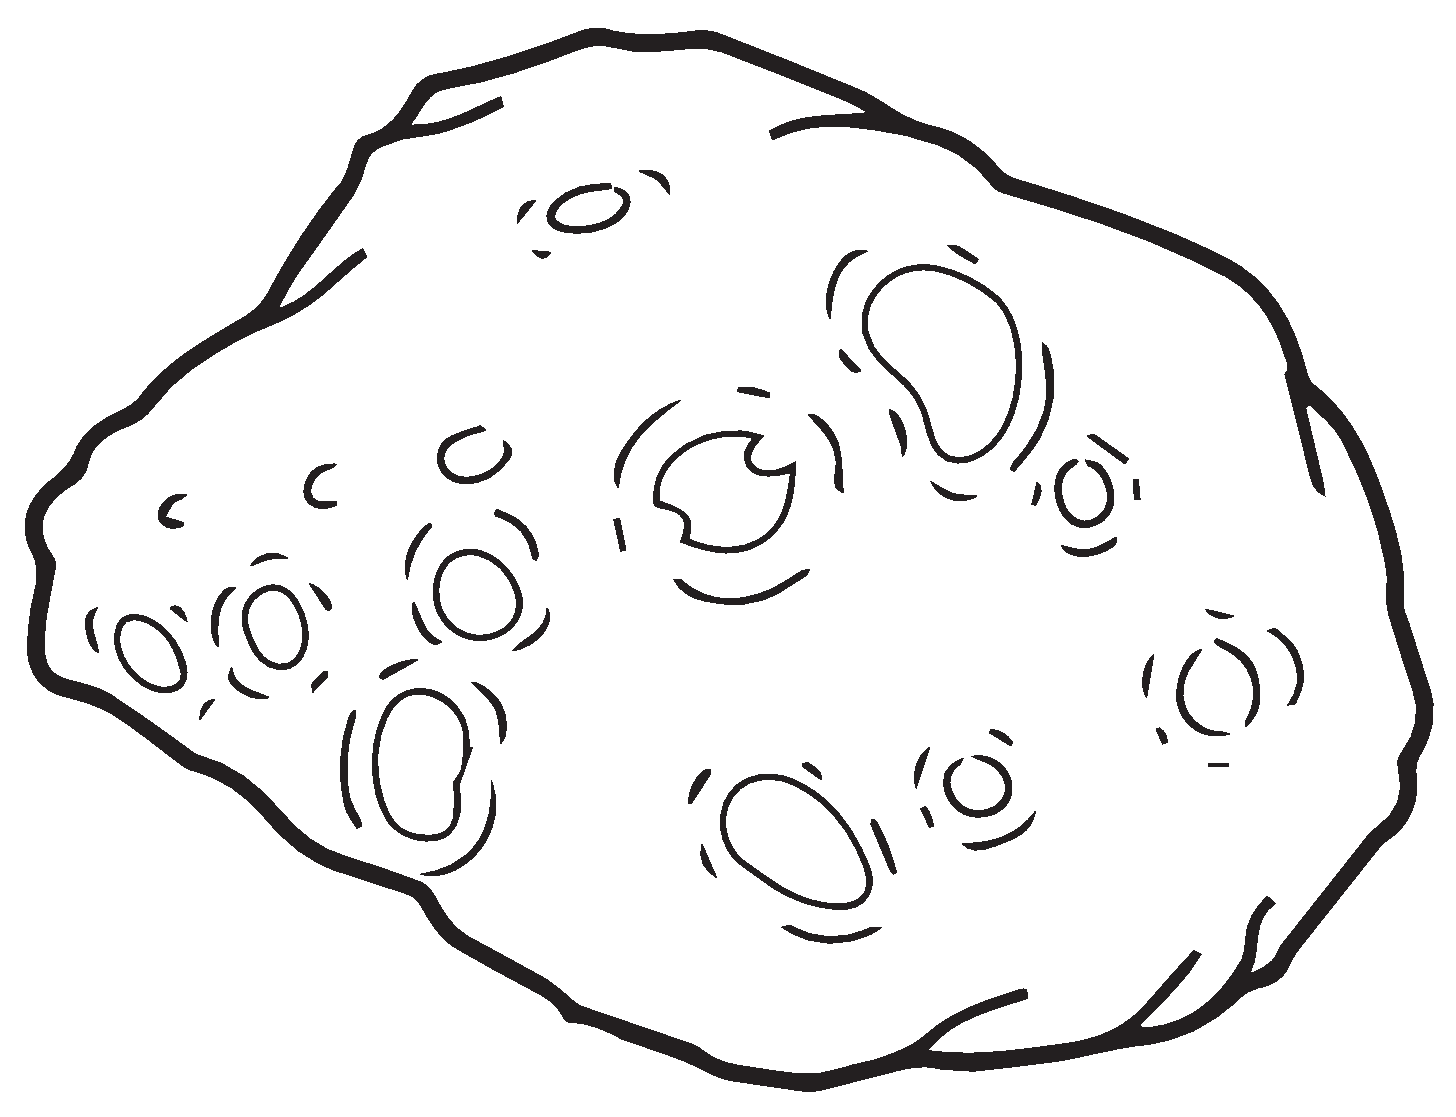
\includegraphics[width=3cm]{asteroid.eps}} node[right=1.5cm] {--- $b$};
		\draw[dashed,thick,-Stealth] (0,-4) -- (0,-1.1);
		\draw (2,-4) node {--- $a$};
		\node[inner sep=0pt] (alien) at (-3.7,0) {
\includegraphics[width=1.8cm]{alien.eps}};
		\draw[thick,-Stealth] (-3,0) -- (-1.5,0);
	\end{tikzpicture}
\end{center}

\begin{fnt}
	\label{fnt7.2.1-3}

Draw the path of the asteroid \textbf{after} the alien applies the force.
\end{fnt}

\begin{enumerate}
	\item On the board, make a \pchart{} for this phenomenon taking the initial point to be just before the push and the final point to be just after the push.
		\label{act7.2.2-2a}
	\item On the board, make a second \pchart{} for this phenomenon taking the initial point to be the same point as the final point in \eqref{act7.2.2-2a} and the final point to be after the asteroid has traveled some distance.
		\label{act7.2.2-2b}
	\item Use your \pcharts{} to explain the path of the asteroid.
	\item Considering your work above in \eqref{act7.2.2-2a} what is the predominant effect of the push?
\end{enumerate}
\vspace{-6pt}
\WCD
\vspace{6pt}
%\subsection{Asteroid moving in a straight line receives a push at right angles}
%\label{act7.2.2-3}

\begin{fnt}
	\label{fnt7.2.1-4}

Along the path you chose in \ref{fnt7.2.1-3}, how does the speed of the asteroid vary \textbf{after} receiving the ``kick''?  Is the velocity changing in direction? Is it increasing, decreasing or remaining the same in magnitude? Describe the motion.
\end{fnt}

\begin{enumerate}\setcounter{enumi}{4}
	\item On the board, use the appropriate \pchart{} from %\hyperref[act7.2.2-2]{\ref*{act7.2.2-2}}
	\eqref{act7.2.2-2a} and \eqref{act7.2.2-2b}
	 to justify your answer to this FNT.
\end{enumerate}
\vspace{-6pt}
\WCD
\vspace{6pt}
%\subsection{Asteroid moving in a straight line receives a push at right angles}
%\label{act7.2.2-4}

\begin{fnt}
	\label{fnt7.2.1-5}

Identify the forces acting on the asteroid, \textbf{after} the alien is finished applying the force.
\end{fnt}

\begin{enumerate}\setcounter{enumi}{5}
	\item On the board, use the appropriate \pchart{} from %\hyperref[act7.2.2-2]{\ref*{act7.2.2-2}}
	\eqref{act7.2.2-2a} and \eqref{act7.2.2-2b}
	 to make a scaled force diagram to answer this FNT.
\end{enumerate}
\vspace{-6pt}
\WCD

\subsection{A Ball Is Dropped and Bounces}
\label{act7.2.2-5}

\begin{fnt}
	\label{fnt7.2.1-6}

When a rubber ball dropped from rest bounces off the floor, its direction of motion is reversed because
\begin{enumerate}[(a)]
	\item energy of the ball is conserved;
	\item momentum of the ball is conserved;
	\item the floor exerts a force on the ball that stops its fall and then drives it upward;
	\item the floor is in the way and the ball has to keep moving;
	\item none of the above.
\end{enumerate}
\end{fnt}

\noindent On the board, make a \pchart{} (include a force diagram) that helps make sense of this situation and helps you to answer the question in this FNT.

\vspace{6pt}
\WCD









 

	\newpage
	\section{Check for Understanding: Momentum}
\label{act7.2.3}

\begin{overview}

	\textbf{Overview:} In this section, we'll pull everything we've discussed about momentum together to apply our understanding to a few new situations.
	
\end{overview}


\subsection{Collisions in One and Two Dimensions}

\begin{fnt}
	\label{fnt7.1.1-7}

Two asteroids collide head-on and stick together. Before the collision, asteroid A (mass 1,\unit[000]{kg}) moved at \unitfrac[100]{m}{s}, and asteroid B (mass 2,\unit[000]{kg}) moved at \unitfrac[80]{m}{s} in the opposite direction. Use momentum conservation (make a complete \pchart{}) to find the velocity of the asteroids after the collision.
\end{fnt}

\begin{fnt}
	\label{fnt7.2.1-7}

Two asteroids identical to those in \ref{fnt7.1.1-7} collide at right angles and stick together. ``Collide at right angles'' means that their initial velocities were perpendicular to each other. You can assume that Asteroid A initially moved to the right and Asteroid B initially moved up.

Use the \pModel{} (make a complete \pchart{}) to find the velocity (magnitude \emph{and} direction, expressed as the angle with the initial velocity vector of Asteroid A) of the asteroids after the collision.  
\end{fnt}

\begin{fnt}
	\label{fnt7.2.1-8}

Determine the decrease in total kinetic energy $\Delta KE_\text{total}$ of the two asteroids in \ref{fnt7.1.1-7} and \ref{fnt7.2.1-7} when they collide.  If the average specific heat of the material composing the asteroids is assumed to be that of ice (\unitfrac[2.05]{kJ}{kg$\cdot$\textdegree{}C}), by how much does the temperature of the asteroids rise as a result of the collision in each case?
\end{fnt}

\begin{enumerate}
	\item In your group, compare your individually created \pcharts{} for \ref{fnt7.1.1-7} and \ref{fnt7.2.1-7}. Note that you do not need to complete the entire chart to find the final velocity. That is, you don't need to find the change in momentum of each asteroid separately. However, finding the individual changes is a good opportunity to hone your skills with momentum conservation.
	
	\textbf{Note:} You may find it useful to choose an $x$-$y$ coordinate system and fill in the chart for \ref{fnt7.2.1-7} with $x$- and $y$-components.
	
	\item On the board, put up complete \pcharts{} (with equations worked through to numerical values) for the 1-D linear collision and the 2-D collision in these two asteroid collision FNTs.
	
	\item Compare your answers to \ref{fnt7.2.1-8}, come to a consensus, and put your response on the board.
	
	\item \textbf{Extension:} Let's consider the asteroid collision as a ``Many Body Problem:'' Three asteroids collide and stick together. Create a possible \pchart{}.
\end{enumerate}

\WCD

\subsection{Horizontally Thrown and Dropped Balls}

\begin{fnt}
	\label{fnt7.2.1-9}

Throw an object (like a ball) horizontally and observe its motion. You are now going to analyze this motion using conservation of momentum. We assume there is no air friction on the ball. Consider the motion of the ball just after it has left your hand moving in a horizontal direction.

\begin{enumerate}[(a)]
	\item Draw a force diagram for the ball. What direction is the net force?
	
	\item Complete the first two rows in the \pchart{} below. The $\vec{p}_i$ of each successive step will be the $\vec{p}_f$ from the previous step. What is the direction of $\Delta \vec{p}~$?
	\vspace{-8pt}
	\begin{center}
		\begin{tikzpicture}[thin,scale=0.9, every node/.style={transform shape},background rectangle/.style={fill=white}, show background rectangle]
			% draw table
			\draw (0,0) -- (0,3);
			\draw[very thick] (2,0) -- (2,3);
			\draw (4,0) -- (4,3);
			\draw (6,0) -- (6,3);
			\draw (8,0) -- (8,3);
			\draw[dashed] (0,0) -- (8,0);
			\draw[very thick] (0,1) -- (8,1);
			\draw[very thick] (0,2) -- (8,2);
			\draw (0,3) -- (8,3);
			
			% label table
			\node[text width=2cm, align=center] at (1,2.5)
				{Open $\vec{p}$ system};
			\node[text width=2cm, align=center] at (3,2.5)
				{$\vec{p}_i$};
			\node[text width=2cm, align=center] at (5,2.5)
				{$\Delta\vec{p}$};
			\node[text width=2cm, align=center] at (7,2.5)
				{$\vec{p}_f$};
			\node[text width=2cm, align=center] at (1,1.5)
				{Ball $\Delta t_1$};
			\node[text width=2cm, align=center] at (1,0.5)
				{Ball $\Delta t_2$};
				
			% arrows
			\draw[-Stealth] (2.5,1.5) -- (3.5,1.5);
			\draw[-Stealth] (6.5,1.75) -- (7.5,1.25);
			\draw[-Stealth] (2.5,0.75) -- (3.5,0.25);
		\end{tikzpicture}
	\end{center}
	\vspace{-12pt}
	\item Add three more rows to the \pchart{} (just show the three vectors $\vec{p}_i$, $\Delta \vec{p}$, and $\vec{p}_f$). Assume the same time interval for each change such that $\Delta \vec{p}$ will be \nicefrac{1}{5} the length of the initial momentum, $\vec{p}_i$.
	
	\item Why does $\Delta \vec{p}$ stay constant for each step?
	
	\item After you have carefully constructed a series of final momenta, use them and what you know about the relationship of the direction of momentum to the path of an object to construct a sketch of the path of the ball.
\end{enumerate}
\end{fnt}

\begin{fnt}
	\label{fnt7.2.1-10}

Repeat what you did in \ref{fnt7.2.1-9}, but this time do two separate \pcharts{}, one for the horizontal and one for the vertical components of the motion. Describe in words how the motion changes in the two directions. Compare your two sketches from part~(e) in \ref{fnt7.2.1-9} and \ref{fnt7.2.1-10}. Are the paths you constructed the same?
\end{fnt}

\begin{fnt}
	\label{fnt7.2.1-11}

\begin{enumerate}[(a)]
	\item Wrap up what you have done in \ref{fnt7.2.1-9} and \ref{fnt7.2.1-10} by explaining, in as few words as possible, why the ball moves along the path you sketched.
	\item For any object to be moving in a curved path what is necessary about the relationships between $\vec{p}_i$, $\Delta \vec{p}$, $\vec{p}_f$, and $\sum F$?
	\item If $\Delta \vec{p}$ were always perpendicular to $\vec{p}_i$ what type of path would this result in?
\end{enumerate}
\end{fnt}

\begin{enumerate}
	\item In your group, compare your individually created \pcharts{} for \ref{fnt7.2.1-9} and \ref{fnt7.2.1-10} and negotiate a consensus for each one.
	
	\item Put your consensus charts on the board. It is simplest to put one header row, with labels $\vec{p}_i$, $\Delta \vec{p}$, and $\vec{p}_f$, and then start a new row in your chart for each time step.
	
	\item Discuss and be prepared to share with the class your response to the prompt, ``Describe in words how the motion changes in the two directions.'' Compare your diagrams from Part~(e) between the two FNTs. Are the paths you constructed the same? Come to a consensus in your small group on your response to Question~(a) in \ref{fnt7.2.1-11} and be prepared to share it with the whole class.
	
	\item Come to a consensus on Parts~(b) and (c)  in  \ref{fnt7.2.1-11} and be prepared to share them with the whole class.
\end{enumerate}

\WCD

%	\section{Check for Understanding: Momentum}
\label{act7.2.3}

\begin{overview}

	\textbf{Overview:} In this section, we'll pull everything we've discussed about momentum together to apply our understanding to a few new situations.
	
\end{overview}


\subsection{Collisions in One and Two Dimensions}

\begin{fnt}
	\label{fnt7.1.1-7}

Two asteroids collide head-on and stick together. Before the collision, asteroid A (mass 1,\unit[000]{kg}) moved at \unitfrac[100]{m}{s}, and asteroid B (mass 2,\unit[000]{kg}) moved at \unitfrac[80]{m}{s} in the opposite direction. Use momentum conservation (make a complete \pchart{}) to find the velocity of the asteroids after the collision.
\end{fnt}

\begin{fnt}
	\label{fnt7.2.1-7}

Two asteroids identical to those in \ref{fnt7.1.1-7} collide at right angles and stick together. ``Collide at right angles'' means that their initial velocities were perpendicular to each other. You can assume that Asteroid A initially moved to the right and Asteroid B initially moved up.

Use the \pModel{} (make a complete \pchart{}) to find the velocity (magnitude \emph{and} direction, expressed as the angle with the initial velocity vector of Asteroid A) of the asteroids after the collision.  
\end{fnt}

\begin{fnt}
	\label{fnt7.2.1-8}

Determine the decrease in total kinetic energy $\Delta KE_\text{total}$ of the two asteroids in \ref{fnt7.1.1-7} and \ref{fnt7.2.1-7} when they collide.  If the average specific heat of the material composing the asteroids is assumed to be that of ice (\unitfrac[2.05]{kJ}{kg$\cdot$\textdegree{}C}), by how much does the temperature of the asteroids rise as a result of the collision in each case?
\end{fnt}

\begin{enumerate}
	\item In your group, compare your individually created \pcharts{} for \ref{fnt7.1.1-7} and \ref{fnt7.2.1-7}. Note that you do not need to complete the entire chart to find the final velocity. That is, you don't need to find the change in momentum of each asteroid separately. However, finding the individual changes is a good opportunity to hone your skills with momentum conservation.
	
	\textbf{Note:} You may find it useful to choose an $x$-$y$ coordinate system and fill in the chart for \ref{fnt7.2.1-7} with $x$- and $y$-components.
	
	\item On the board, put up complete \pcharts{} (with equations worked through to numerical values) for the 1-D linear collision and the 2-D collision in these two asteroid collision FNTs.
	
	\item Compare your answers to \ref{fnt7.2.1-8}, come to a consensus, and put your response on the board.
	
	\item \textbf{Extension:} Let's consider the asteroid collision as a ``Many Body Problem:'' Three asteroids collide and stick together. Create a possible \pchart{}.
\end{enumerate}

\WCD

\subsection{Horizontally Thrown and Dropped Balls}

\begin{fnt}
	\label{fnt7.2.1-9}

Throw an object (like a ball) horizontally and observe its motion. You are now going to analyze this motion using conservation of momentum. We assume there is no air friction on the ball. Consider the motion of the ball just after it has left your hand moving in a horizontal direction.

\begin{enumerate}[(a)]
	\item Draw a force diagram for the ball. What direction is the net force?
	
	\item Complete the first two rows in the \pchart{} below. The $\vec{p}_i$ of each successive step will be the $\vec{p}_f$ from the previous step. What is the direction of $\Delta \vec{p}~$?
	\vspace{-8pt}
	\begin{center}
		\begin{tikzpicture}[thin,scale=0.9, every node/.style={transform shape},background rectangle/.style={fill=white}, show background rectangle]
			% draw table
			\draw (0,0) -- (0,3);
			\draw[very thick] (2,0) -- (2,3);
			\draw (4,0) -- (4,3);
			\draw (6,0) -- (6,3);
			\draw (8,0) -- (8,3);
			\draw[dashed] (0,0) -- (8,0);
			\draw[very thick] (0,1) -- (8,1);
			\draw[very thick] (0,2) -- (8,2);
			\draw (0,3) -- (8,3);
			
			% label table
			\node[text width=2cm, align=center] at (1,2.5)
				{Open $\vec{p}$ system};
			\node[text width=2cm, align=center] at (3,2.5)
				{$\vec{p}_i$};
			\node[text width=2cm, align=center] at (5,2.5)
				{$\Delta\vec{p}$};
			\node[text width=2cm, align=center] at (7,2.5)
				{$\vec{p}_f$};
			\node[text width=2cm, align=center] at (1,1.5)
				{Ball $\Delta t_1$};
			\node[text width=2cm, align=center] at (1,0.5)
				{Ball $\Delta t_2$};
				
			% arrows
			\draw[-Stealth] (2.5,1.5) -- (3.5,1.5);
			\draw[-Stealth] (6.5,1.75) -- (7.5,1.25);
			\draw[-Stealth] (2.5,0.75) -- (3.5,0.25);
		\end{tikzpicture}
	\end{center}
	\vspace{-12pt}
	\item Add three more rows to the \pchart{} (just show the three vectors $\vec{p}_i$, $\Delta \vec{p}$, and $\vec{p}_f$). Assume the same time interval for each change such that $\Delta \vec{p}$ will be \nicefrac{1}{5} the length of the initial momentum, $\vec{p}_i$.
	
	\item Why does $\Delta \vec{p}$ stay constant for each step?
	
	\item After you have carefully constructed a series of final momenta, use them and what you know about the relationship of the direction of momentum to the path of an object to construct a sketch of the path of the ball.
\end{enumerate}
\end{fnt}

\begin{fnt}
	\label{fnt7.2.1-10}

Repeat what you did in \ref{fnt7.2.1-9}, but this time do two separate \pcharts{}, one for the horizontal and one for the vertical components of the motion. Describe in words how the motion changes in the two directions. Compare your two sketches from part~(e) in \ref{fnt7.2.1-9} and \ref{fnt7.2.1-10}. Are the paths you constructed the same?
\end{fnt}

\begin{fnt}
	\label{fnt7.2.1-11}

\begin{enumerate}[(a)]
	\item Wrap up what you have done in \ref{fnt7.2.1-9} and \ref{fnt7.2.1-10} by explaining, in as few words as possible, why the ball moves along the path you sketched.
	\item For any object to be moving in a curved path what is necessary about the relationships between $\vec{p}_i$, $\Delta \vec{p}$, $\vec{p}_f$, and $\sum F$?
	\item If $\Delta \vec{p}$ were always perpendicular to $\vec{p}_i$ what type of path would this result in?
\end{enumerate}
\end{fnt}

\begin{enumerate}
	\item In your group, compare your individually created \pcharts{} for \ref{fnt7.2.1-9} and \ref{fnt7.2.1-10} and negotiate a consensus for each one.
	
	\item Put your consensus charts on the board. It is simplest to put one header row, with labels $\vec{p}_i$, $\Delta \vec{p}$, and $\vec{p}_f$, and then start a new row in your chart for each time step.
	
	\item Discuss and be prepared to share with the class your response to the prompt, ``Describe in words how the motion changes in the two directions.'' Compare your diagrams from Part~(e) between the two FNTs. Are the paths you constructed the same? Come to a consensus in your small group on your response to Question~(a) in \ref{fnt7.2.1-11} and be prepared to share it with the whole class.
	
	\item Come to a consensus on Parts~(b) and (c)  in  \ref{fnt7.2.1-11} and be prepared to share them with the whole class.
\end{enumerate}

\WCD %B
%	\newpage
%	\input{U7/act7.3.1}


%%%%%%%%%%%%%%%%%%%%%%%%%%%%%%%%%%%%%%%%%%%%%%%%%%%%%%%%%%%%%%%%%%%%%%%%
%
%		DLM 14
%
%%%%%%%%%%%%%%%%%%%%%%%%%%%%%%%%%%%%%%%%%%%%%%%%%%%%%%%%%%%%%%%%%%%%%%%%

%\chapter[\chaptername\thechapter]{\chapterlongname \thechapter}
%\label{dlm14}
%\addchapter

%	\input{U7/act7.3.5}
%	\newpage
%	\input{U7/act7.3.3}
%	\newpage
%	\input{U7/act7.3.4}


%%%%%%%%%%%%%%%%%%%%%%%%%%%%%%%%%%%%%%%%%%%%%%%%%%%%%%%%%%%%%%%%%%%%%%%%
%
%		DLM 15
%
%%%%%%%%%%%%%%%%%%%%%%%%%%%%%%%%%%%%%%%%%%%%%%%%%%%%%%%%%%%%%%%%%%%%%%%%

%\chapter[\chaptername\thechapter]{\chapterlongname \thechapter}
%\label{dlm15}
%\addchapter

%%	\input{U7/act7.3.5}
%%	\newpage
%%	\input{U7/act7.3.3}
%%	\newpage
%%	\input{U7/act7.3.4}


%%%%%%%%%%%%%%%%%%%%%%%%%%%%%%%%%%%%%%%%%%%%%%%%%%%%%%%%%%%%%%%%%%%%%%%%
%
%		DLM 16A
%
%%%%%%%%%%%%%%%%%%%%%%%%%%%%%%%%%%%%%%%%%%%%%%%%%%%%%%%%%%%%%%%%%%%%%%%%

%\chapter[\chaptername\thechapter]{\chapterlongname \thechapter}
%\label{dlm16a}
%\addchapter

%%	\input{U7/act7.3.5}
%%	\newpage
%%	\input{U7/act7.3.3}
%%	\newpage
%%	\input{U7/act7.3.4}


%%%%%%%%%%%%%%%%%%%%%%%%%%%%%%%%%%%%%%%%%%%%%%%%%%%%%%%%%%%%%%%%%%%%%%%%
%
%		DLM 16B
%
%%%%%%%%%%%%%%%%%%%%%%%%%%%%%%%%%%%%%%%%%%%%%%%%%%%%%%%%%%%%%%%%%%%%%%%%

%\chapter[\chaptername\thechapter]{\chapterlongname \thechapter}
%\label{dlm16b}
%\addchapter

%	\input{U7/fnt7.3.2-3}
%	\newpage
%	\input{U7/practice-quiz-10}
%	\newpage
%	\label{fnt8.1.1-1}

\textbf{Cart and Horse Paradox:} If a horse pulls on a cart, and the cart pulls back on the horse with an equal magnitude force, how can either possibly begin to move?

Use what you have learned about force to \textbf{give a complete explanation of this paradox.} For a complete explanation, make and refer to complete \forcediags{} for each of the following.
\begin{enumerate}[(a)]
	\item the horse, 
	\item the cart, and 
	\item the whole system (horse \& cart).
\end{enumerate}
%	\newpage
%	\label{fnt8.1.1-2}

\begin{wrapfigure}{R}{0.25\textwidth}
	\vspace{-37pt}
  	\centering
	\begin{center}
	\begin{tikzpicture}[thick,scale=0.9, every node/.style={transform shape},background rectangle/.style={fill=white}, show background rectangle]
		\node[inner sep=0pt,rotate=-20] (fingers) at (-.7,4.3) {
\includegraphics[width=2cm]{pinchedFingers.png}};
		\node at (0,0) {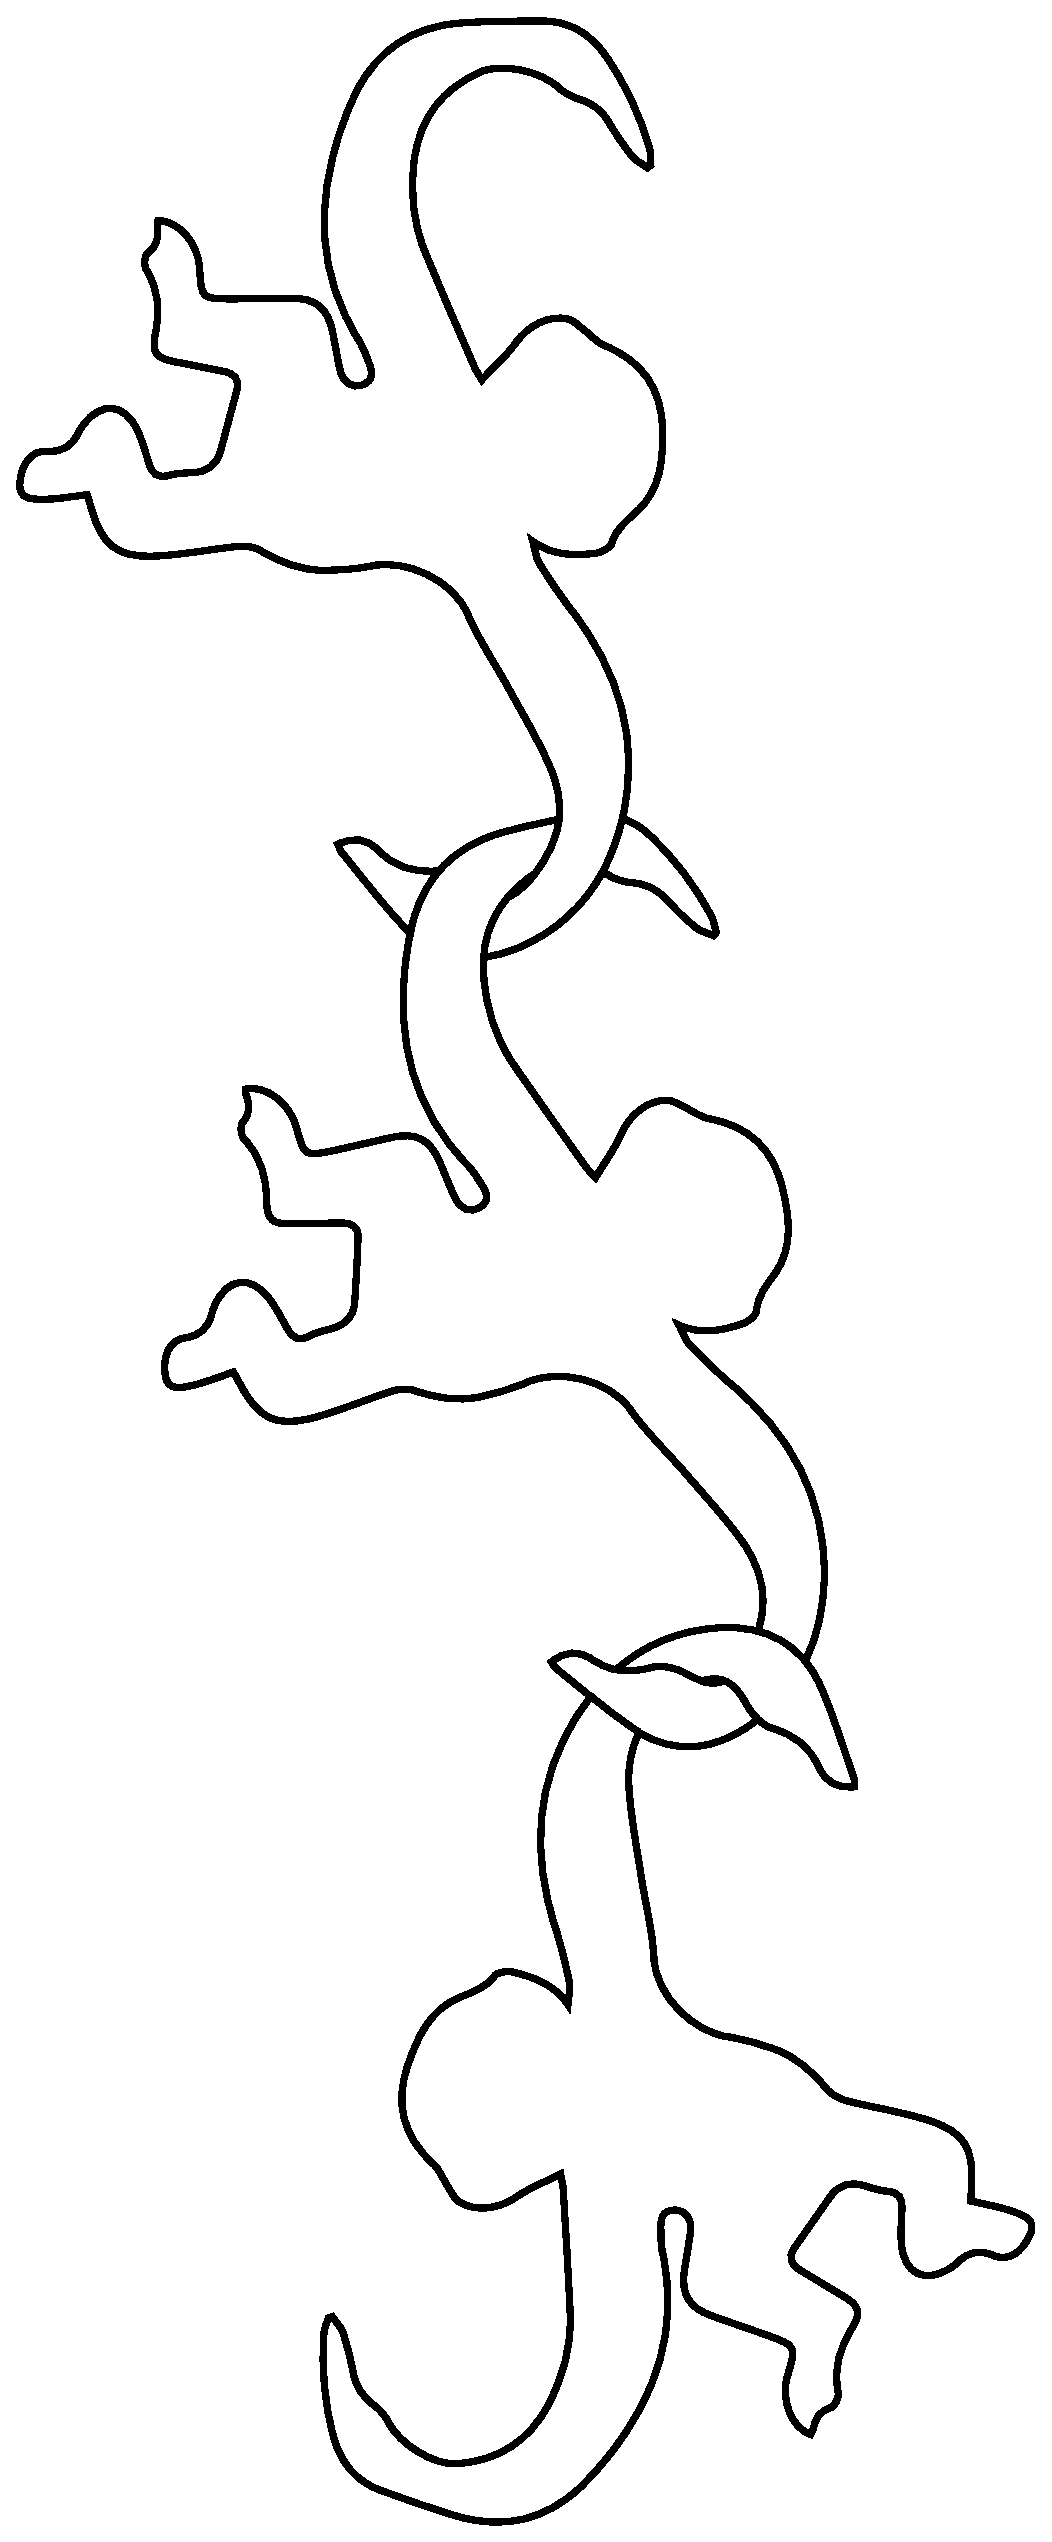
\includegraphics[width=3cm]{barrelmonkey.eps}};
		\node at (-0.25,2.4) {\scriptsize{$m=\unit[40]{g}$}};
		\node[rotate=2] at (0.12,0.1) {\scriptsize{$m=\unit[30]{g}$}};
		\node[rotate=-20] at (0.3,-2.5) {\scriptsize{$m=\unit[20]{g}$}};
	\end{tikzpicture}
	\vspace{20pt}
	\end{center}
\end{wrapfigure}

\noindent Your little brother is playing with monkeys in a barrel. The mass of each monkey is indicated in the illustration on the right. Note that your brother is holding the monkeys still and his hand weighs \unit[50]{N}.

\begin{enumerate}[(a)]
	\item Make a separate \forcediag{} for each of the four objects, the hand, top monkey, middle monkey, bottom monkey.
	
	\item Identify all 3rd law pairs of forces appearing in your \forcediags{} by circling the two forces and connecting them with a line.
	
	\item Use Newton's 1st and 3rd laws to numerically determine all of the forces acting on the monkeys and the hand. If necessary, redraw your \forcediags{}, so they are more to scale.
\end{enumerate}
%	\newpage
%	\section{Newton's Laws and Momentum Conservation}
\label{act8.1.1}

\begin{overview}

	\textbf{Overview:} Over the past few weeks, we've dealt a lot with forces, and we know much more about motion in general. We even know that forces cause changes in motion. Sir Isaac Newton, a physicist of the 17th/18th century, formulated three famous laws that powerfully express the relationship between forces and motion. In this next section, we'll discuss these so-called \emph{Newton's Laws}.

\end{overview}

\subsection{Getting started with Newton's Laws}

\begin{fnt}
	\label{8.1.0-1}

\textbf{A puzzle to think about:} Two weights of mass \unit[1]{kg} hang from strings which go over pulleys (see illustration below). The strings are attached to the two ends of a spring scale which reads the force. Does the scale read \unit[0]{N}, \unit[9.8]{N}, or \unit[19.6]{N}? Why?\\

\vspace{-10pt}
\begin{center}
	\begin{tikzpicture}[thin,scale=1, every node/.style={transform shape},background rectangle/.style={fill=white}, show background rectangle]
		%table
		\draw (2,3) rectangle (10,3.5);
		\draw (3,0) rectangle (3.25,3);
		\draw (8.75,0) rectangle (9,3);
		%pulleys
		\draw (1.5,3.62) circle (.3);
		\draw (10.5,3.62) circle (.3);
		\filldraw[fill=white,draw=black] (1.5,3.5) rectangle (2.5,3.7);
		\filldraw[fill=white,draw=black] (9.5,3.5) rectangle (10.5,3.7);
		%weights
		\draw (.8,1.5) rectangle (1.6,2) node[midway] {\unit[1]{kg}};
		\draw (10.4,1.5) rectangle (11.2,2) node[midway] {\unit[1]{kg}};
		%string
		\draw (1.2,2) -- (1.2,3.62);
		\draw (10.8,2) -- (10.8,3.62);
		\draw (1.5,3.92) -- (5.3,3.92);
		\draw (10.5,3.92) -- (6.9,3.92);
		%spring scale
		\draw (5.5,3.72) rectangle (6.5,4.12) node[midway,above=6pt] {\scriptsize{Spring Scale}};
		\foreach \x in {5.7, 5.9, 6.1, 6.3}
			\draw (\x,3.8) -- (\x,4.04);
		\draw (5.4,3.92) circle (.1);
		\draw (6.7,3.92) ellipse (.2 and .1);
	\end{tikzpicture}
\end{center}

\noindent\textbf{Hint:} Draw a \forcediag{} for the scale in this situation and then draw a \forcediag{} for the scale when it is being used to weigh a hanging object with mass \unit[1]{kg}.
\end{fnt}

\WCD

\newpage

\subsection{Newton's Laws and the \pConsModel{}}

\begin{reading}
\textbf{\textit{Newton's Three Laws of Motion}}

\begin{enumerate}[I.]
	\item Without a net force, there can be no change in the velocity of an object:\footnote{This can be expressed as ``An object in motion remains in motion in a straight line forever unless acted on by an external force;'' and ``An object at rest remains at rest forever unless acted on by an external force.''}
	
	\begin{center}\framebox[1.1\width][c]{If $\sum\vec{F}=0$, then $\Delta\vec{v}=0$.}\end{center}
	
	\item An object will be accelerated if there is a net force acting upon it:
	
	\begin{center}\framebox[1.1\width][c]{$\sum\vec{F}=m\vec{a}$}\end{center}

	\item If object $A$ exerts a force on object $B$, object $B$ \emph{simultaneously} exerts an equal and opposite force on object $A$:\footnote{You may have heard of this as ``For every action, there is an equal and opposite reaction.''}
	
	\begin{center}\framebox[1.1\width][c]{$\vec{F}_\text{A on B} = -\vec{F}_\text{B on A}$}\end{center}
	
\end{enumerate}

\end{reading}

\begin{enumerate}
	\item Come up with a physical scenario that illustrates each of Newton's three laws. Describe each law in both sentence form and with a concise mathematical expression, specific to your example. Be careful and precise with notation in the algebraic expressions.
	
	\item 
	  % We have to create a parbox here because wrapfigure does not support enumerate environments directly
	  \parbox[t]{\dimexpr\textwidth-\leftmargin}{%
      \vspace{-3mm}
      \begin{wrapfigure}[6]{r}{5cm}
        \centering
        \vspace{-\baselineskip}
			\begin{tikzpicture}[scale=.8, every node/.style={transform shape}]{r}{1}
				\draw[blue] (0,0) ellipse (0.75cm and 0.33cm);
				\draw[blue] (3,1.5) ellipse (0.75cm and 0.33cm);
				\draw[blue,dashed] (1,0) .. controls (2.25,0.25) .. (2.75,1) node[midway, right=4pt, blue] {3rd law};
			\end{tikzpicture}
	  \end{wrapfigure}
      Make a \forcediag{} for each object in each of the following situations. For each situation, circle and connect the forces that are in tandem as third law pairs, as shown.
      }
	
	\begin{enumerate}
		\item Refer to the %rocket example of \ref{fnt7.1.1-2}.
		astronaut example from \ref{14C.1}. 
		Recreate a \pchart{} and follow the instructions for the force diagram above. Explain how each of Newton's Laws can be identified in the \pcharts{} and \forcediags{}. Suppose we wanted the rocket to move at a constant speed, is a net force necessary to make this happen?
		
		\item Refer to the boat example of \ref{fnt7.1.1-3}. Recreate a \pchart{} and follow the instructions for the force diagram above. Explain how each of Newton's Laws can be identified in the \pcharts{} and \forcediags{}.
	\end{enumerate}
\end{enumerate}

\WCD

\subsection{Use Newton's Three Laws applied to a system of three objects}

\subsubsection*{\emph{Static} Case: All objects sitting still}

\begin{enumerate}
	\item Refer to the picture below of three books sitting on a table that is standing on a floor. Make a separate \forcediag{} for each of the four objects: Books~A, B, and C, and the table. The masses of the books are \unit[0.8]{kg}, \unit[0.2]{kg}, and \unit[0.5]{kg} for Books~A, B, and C, respectively and the mass of the table is \unit[30]{kg}.
	
	\begin{center}
	\begin{tikzpicture}{c}{1}
		% Table
		\draw[double distance = 5pt] (1,0) -- (1,2);
		\draw[double distance = 5pt] (4,0) -- (4,2);
		\draw (0.5,2) rectangle (4.5,2.5) node[midway] {table};
		% Book C
		\draw (1.75,2.5) rectangle (3.5,3.25) node[midway] {C};
		% Book B
		\draw (2,3.25) rectangle (3.25,3.75) node[midway] {B};
		% Book A
		\draw (1.25,3.75) rectangle (3.75,4.5) node[midway] {A};
		% Floor
		\draw (0,0) -- (5,0);
		\foreach \x in {0.5,1,1.5,2,2.5,3,3.5,4,4.5,5}
    			\draw (\x,0) -- (\x-0.25,-0.25);
	\end{tikzpicture}
	\end{center}
	
	\item Identify all 3rd law pairs of forces appearing in your \forcediags{} by circling the two forces and connecting as shown in the diagram on the previous page.
	
	\item Use Newton's 1st and 3rd laws to numerically determine all of the forces acting on the books and the table. If necessary, redraw your \forcediags{} so they are more to scale.
\end{enumerate}

\subsubsection*{\emph{Dynamic} Cases: Objects moving horizontally and vertically}

\begin{enumerate}
	  \setcounter{enumi}{3}
	\item If the books and table together are sliding across the room each at the same constant speed, how would your \forcediags{} change? Show precisely how it would change or explain why it would not.
	
	\item Now imagine the table is sitting in an elevator that begins to accelerate upward with an acceleration equal to $\unitfrac[2]{m}{s^2}$.
	\begin{enumerate}
		\item Make a new \forcediag{} for each book and determine the forces acting on it.
		\item Create a \pchart{} for at least two of the objects.
		\item Do any of the objects experience a net force? If so, give the magnitude and direction of each.
		\item Is it correct to say a force always equals $m\vec{a}$~?
	\end{enumerate}
\end{enumerate}

\WCD

\subsection{Applications of Newton's Laws}

\begin{fnt}
	\label{fnt8.1.1-2}

\begin{wrapfigure}{R}{0.25\textwidth}
	\vspace{-37pt}
  	\centering
	\begin{center}
	\begin{tikzpicture}[thick,scale=0.9, every node/.style={transform shape},background rectangle/.style={fill=white}, show background rectangle]
		\node[inner sep=0pt,rotate=-20] (fingers) at (-.7,4.3) {
\includegraphics[width=2cm]{pinchedFingers.png}};
		\node at (0,0) {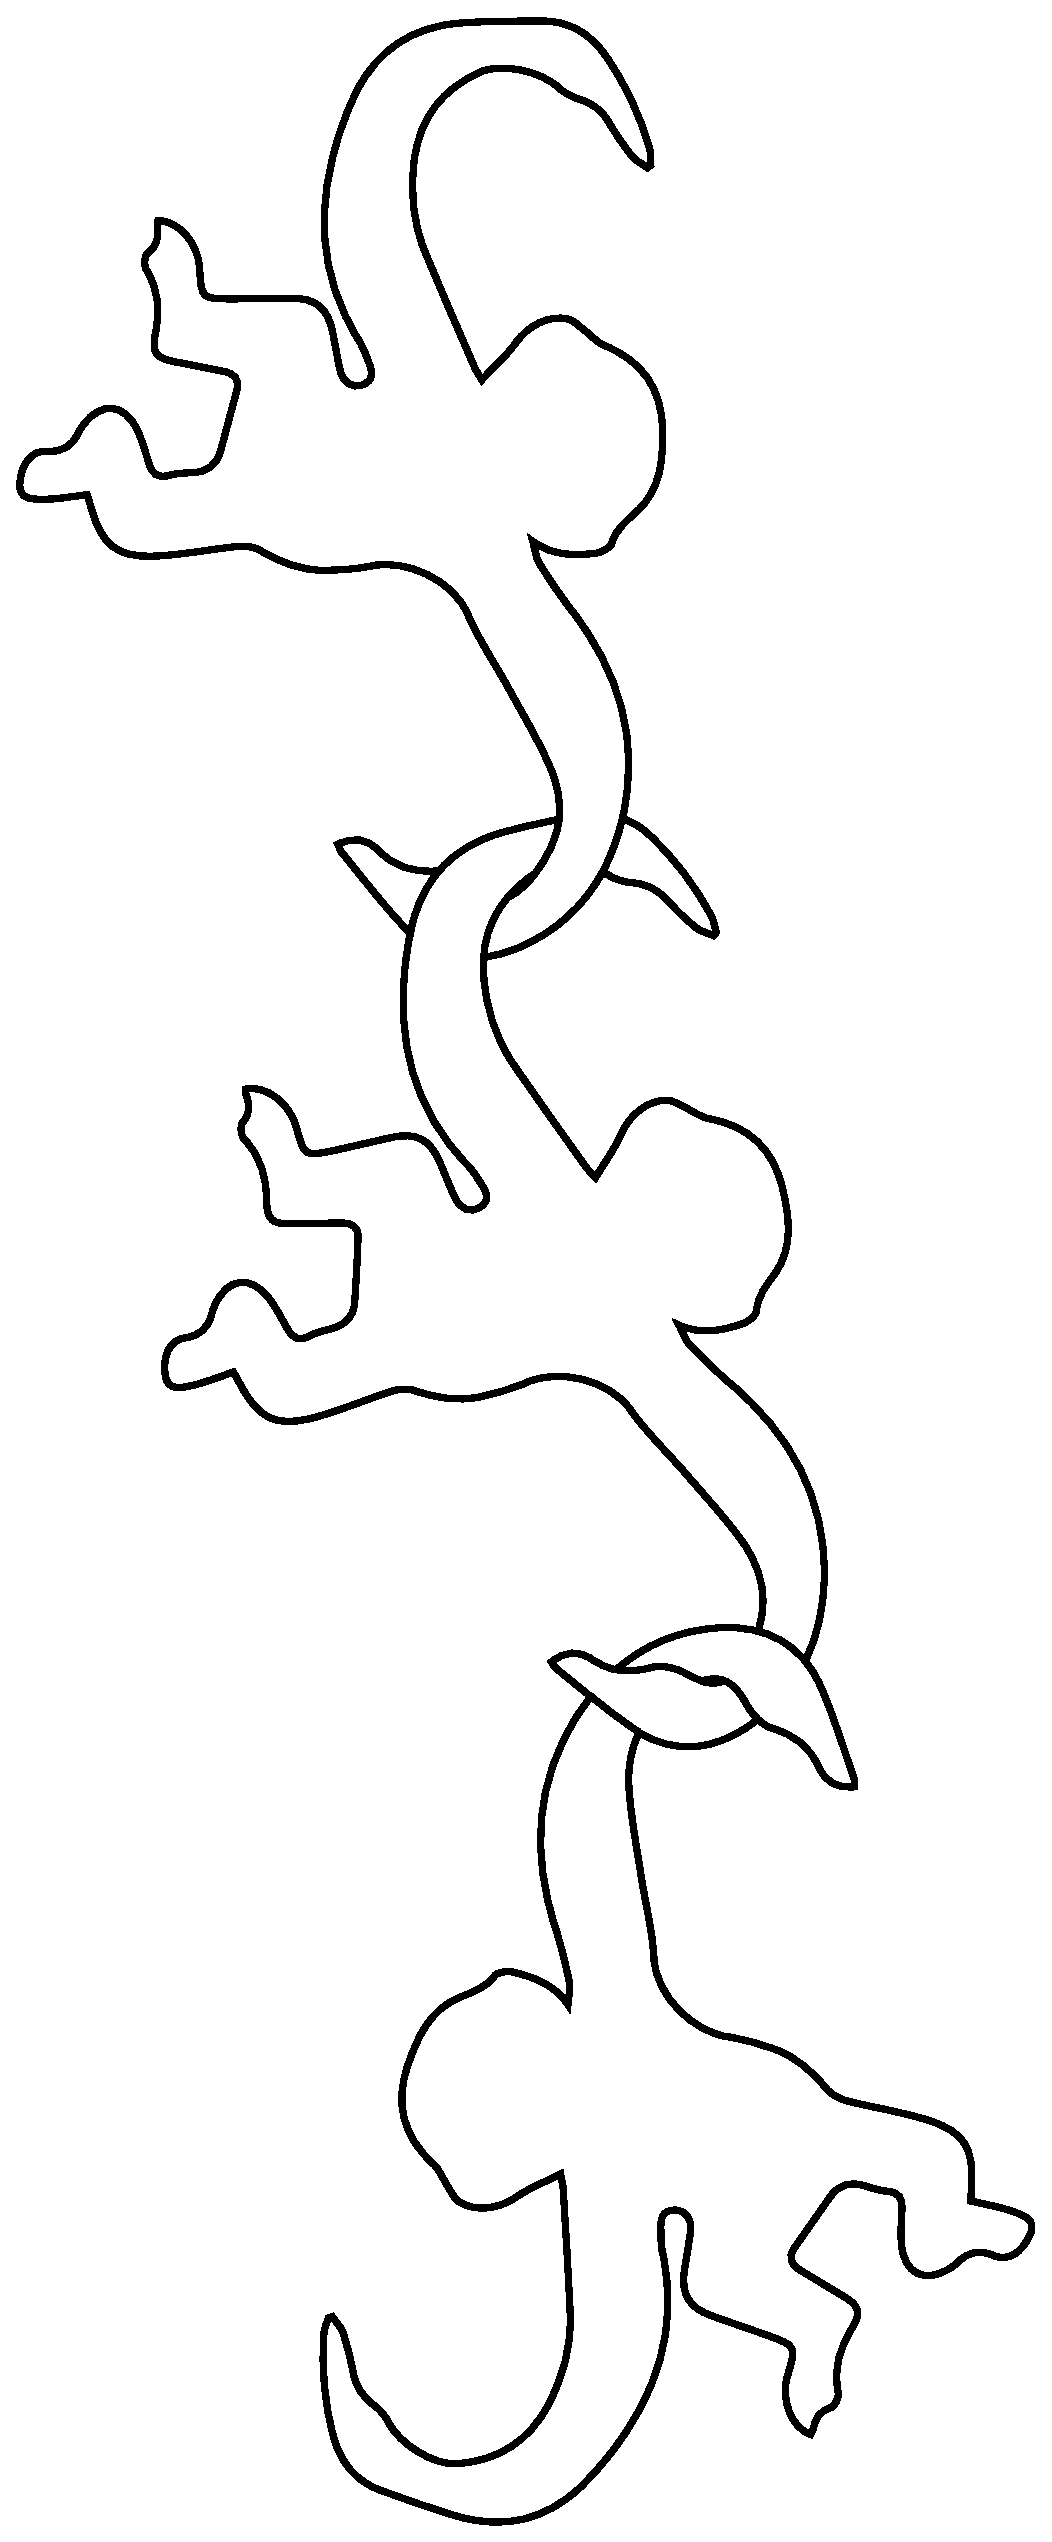
\includegraphics[width=3cm]{barrelmonkey.eps}};
		\node at (-0.25,2.4) {\scriptsize{$m=\unit[40]{g}$}};
		\node[rotate=2] at (0.12,0.1) {\scriptsize{$m=\unit[30]{g}$}};
		\node[rotate=-20] at (0.3,-2.5) {\scriptsize{$m=\unit[20]{g}$}};
	\end{tikzpicture}
	\vspace{20pt}
	\end{center}
\end{wrapfigure}

\noindent Your little brother is playing with monkeys in a barrel. The mass of each monkey is indicated in the illustration on the right. Note that your brother is holding the monkeys still and his hand weighs \unit[50]{N}.

\begin{enumerate}[(a)]
	\item Make a separate \forcediag{} for each of the four objects, the hand, top monkey, middle monkey, bottom monkey.
	
	\item Identify all 3rd law pairs of forces appearing in your \forcediags{} by circling the two forces and connecting them with a line.
	
	\item Use Newton's 1st and 3rd laws to numerically determine all of the forces acting on the monkeys and the hand. If necessary, redraw your \forcediags{}, so they are more to scale.
\end{enumerate}
\end{fnt}

\vspace{-6pt}
\WCD
\vspace{12pt}

%\section{Some things to ponder before we begin}
\label{act8.1.0-part2}

\begin{fnt}
	\input{U8/fnt8.1.0-2}
\end{fnt}

\vspace{-6pt}
\WCD

%We'll skip this one...
%\begin{fnt}
%	\input{U8/fnt8.1.1-3}
%\end{fnt}

%\WCD

%\begin{fnt}
%	\input{U8/fnt8.1.1-4}
%\end{fnt}
%
%\WCD
	\label{Unit7}

\part[Forces and Motion: Newton's Laws]{Forces and Motion:\\ The \FModel{}}
	%%%%%%%%%%%%%%%%%%%%%%%%%%%%%%%%%%%%%%%%%%%%%%%%%%%%%%%%%%%%%%%%%%%%%%%%
%
%		DLM 16B (continued)
%
%%%%%%%%%%%%%%%%%%%%%%%%%%%%%%%%%%%%%%%%%%%%%%%%%%%%%%%%%%%%%%%%%%%%%%%%

\chapter[\chaptername\thechapter]{\chapterlongname \thechapter}
\label{dlm16b}
\addchapter

%	\section{Somethings to ponder before we begin}
\label{act8.1.0}

\begin{fnt}
	\label{8.1.0-1}

\textbf{A puzzle to think about:} Two weights of mass \unit[1]{kg} hang from strings which go over pulleys (see illustration below). The strings are attached to the two ends of a spring scale which reads the force. Does the scale read \unit[0]{N}, \unit[9.8]{N}, or \unit[19.6]{N}? Why?\\

\vspace{-10pt}
\begin{center}
	\begin{tikzpicture}[thin,scale=1, every node/.style={transform shape},background rectangle/.style={fill=white}, show background rectangle]
		%table
		\draw (2,3) rectangle (10,3.5);
		\draw (3,0) rectangle (3.25,3);
		\draw (8.75,0) rectangle (9,3);
		%pulleys
		\draw (1.5,3.62) circle (.3);
		\draw (10.5,3.62) circle (.3);
		\filldraw[fill=white,draw=black] (1.5,3.5) rectangle (2.5,3.7);
		\filldraw[fill=white,draw=black] (9.5,3.5) rectangle (10.5,3.7);
		%weights
		\draw (.8,1.5) rectangle (1.6,2) node[midway] {\unit[1]{kg}};
		\draw (10.4,1.5) rectangle (11.2,2) node[midway] {\unit[1]{kg}};
		%string
		\draw (1.2,2) -- (1.2,3.62);
		\draw (10.8,2) -- (10.8,3.62);
		\draw (1.5,3.92) -- (5.3,3.92);
		\draw (10.5,3.92) -- (6.9,3.92);
		%spring scale
		\draw (5.5,3.72) rectangle (6.5,4.12) node[midway,above=6pt] {\scriptsize{Spring Scale}};
		\foreach \x in {5.7, 5.9, 6.1, 6.3}
			\draw (\x,3.8) -- (\x,4.04);
		\draw (5.4,3.92) circle (.1);
		\draw (6.7,3.92) ellipse (.2 and .1);
	\end{tikzpicture}
\end{center}

\noindent\textbf{Hint:} Draw a \forcediag{} for the scale in this situation and then draw a \forcediag{} for the scale when it is being used to weigh a hanging object with mass \unit[1]{kg}.
\end{fnt}

\WCD

%\begin{fnt}
%	\label{fnt8.1.1-1}

\textbf{Cart and Horse Paradox:} If a horse pulls on a cart, and the cart pulls back on the horse with an equal magnitude force, how can either possibly begin to move?

Use what you have learned about force to \textbf{give a complete explanation of this paradox.} For a complete explanation, make and refer to complete \forcediags{} for each of the following.
\begin{enumerate}[(a)]
	\item the horse, 
	\item the cart, and 
	\item the whole system (horse \& cart).
\end{enumerate}
%\end{fnt}
%
%\WCD

\begin{fnt}
	\label{fnt8.1.1-2}

\begin{wrapfigure}{R}{0.25\textwidth}
	\vspace{-37pt}
  	\centering
	\begin{center}
	\begin{tikzpicture}[thick,scale=0.9, every node/.style={transform shape},background rectangle/.style={fill=white}, show background rectangle]
		\node[inner sep=0pt,rotate=-20] (fingers) at (-.7,4.3) {
\includegraphics[width=2cm]{pinchedFingers.png}};
		\node at (0,0) {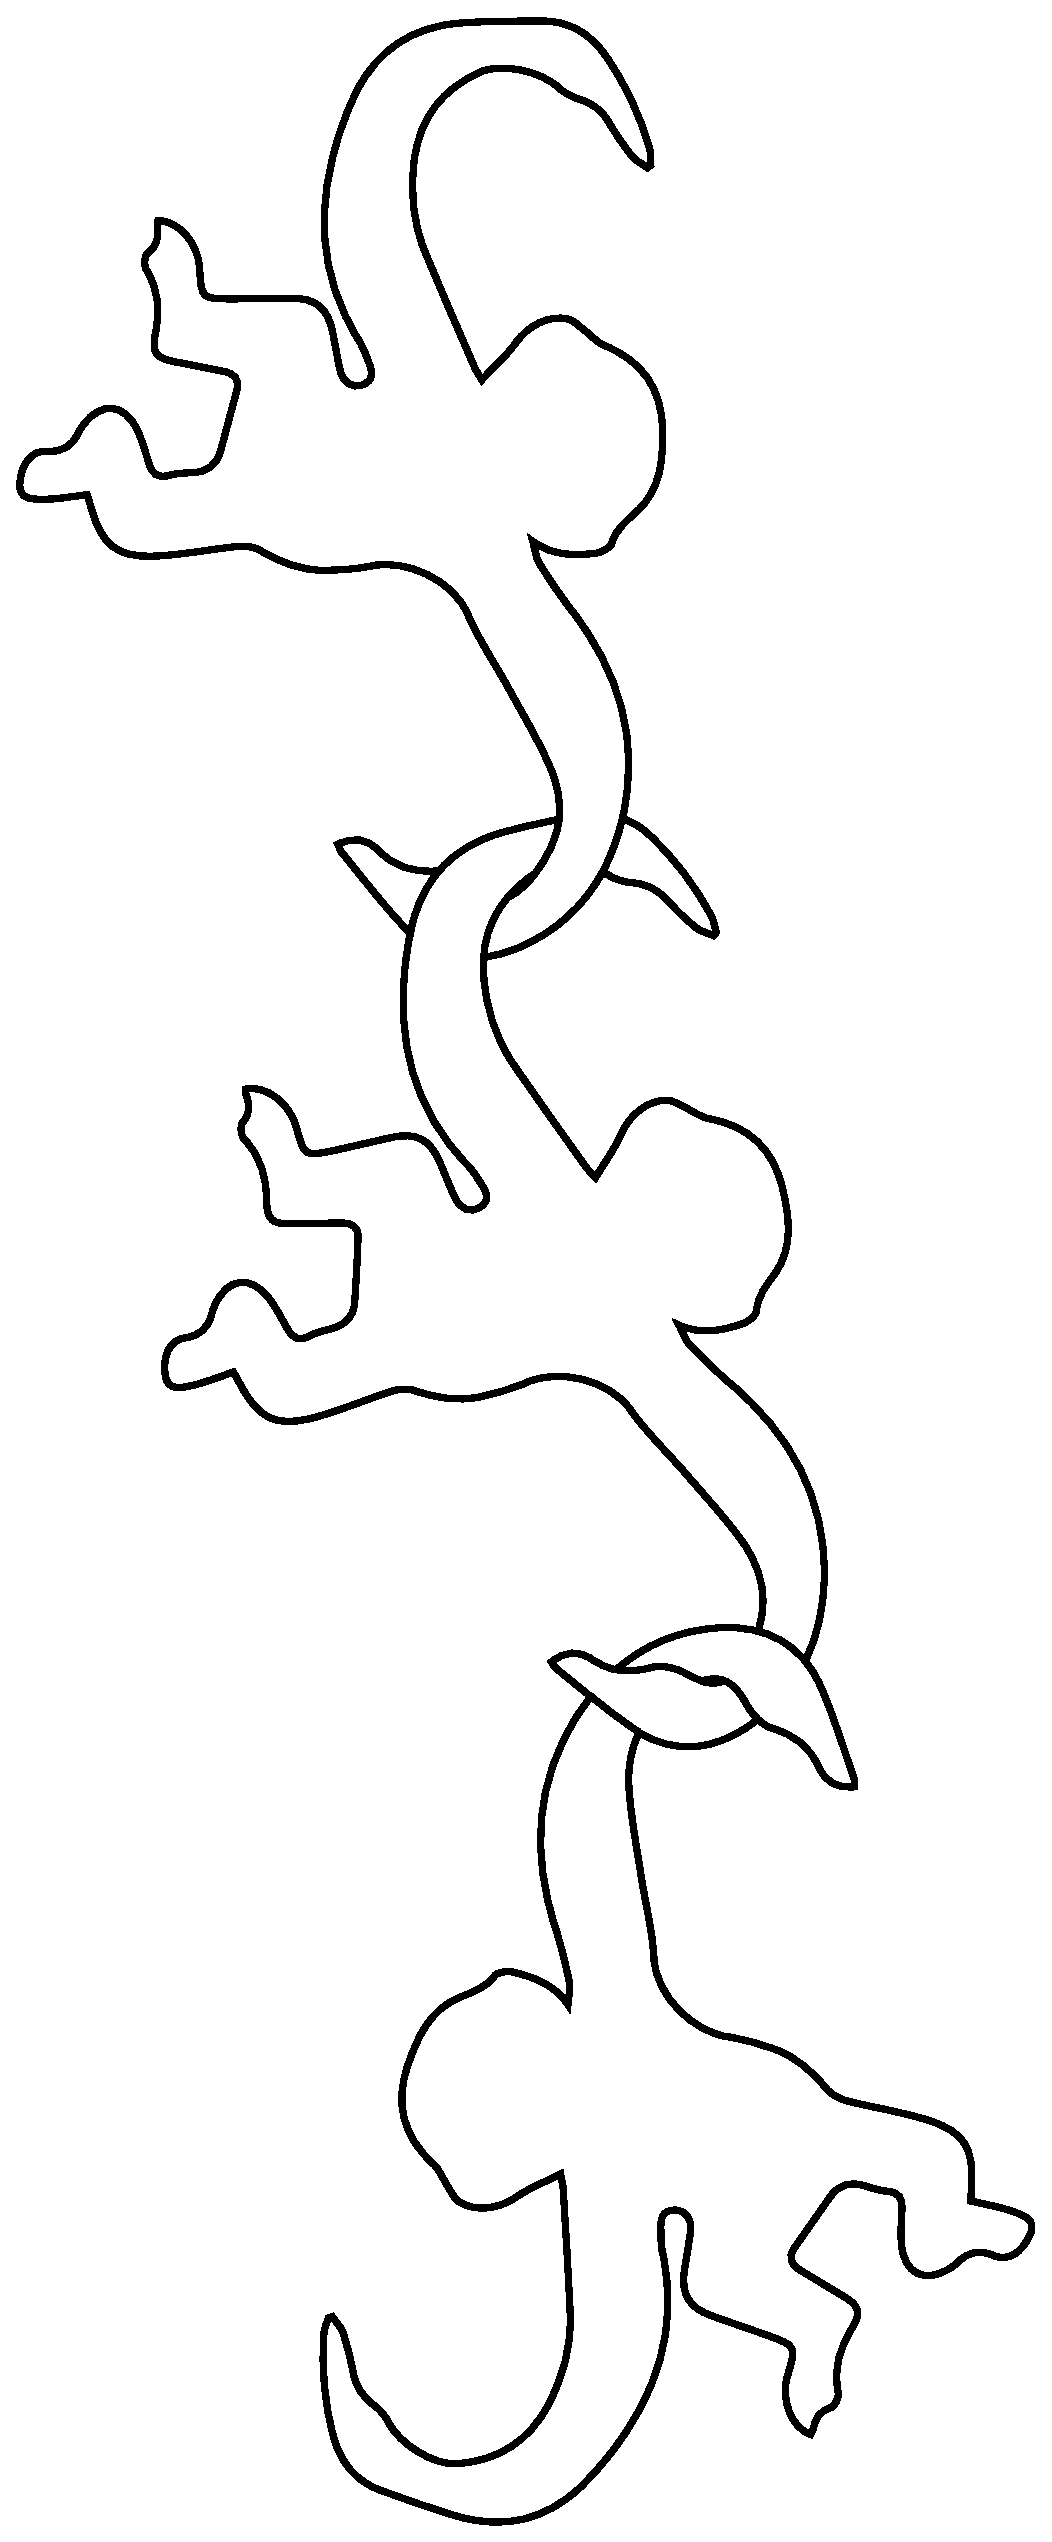
\includegraphics[width=3cm]{barrelmonkey.eps}};
		\node at (-0.25,2.4) {\scriptsize{$m=\unit[40]{g}$}};
		\node[rotate=2] at (0.12,0.1) {\scriptsize{$m=\unit[30]{g}$}};
		\node[rotate=-20] at (0.3,-2.5) {\scriptsize{$m=\unit[20]{g}$}};
	\end{tikzpicture}
	\vspace{20pt}
	\end{center}
\end{wrapfigure}

\noindent Your little brother is playing with monkeys in a barrel. The mass of each monkey is indicated in the illustration on the right. Note that your brother is holding the monkeys still and his hand weighs \unit[50]{N}.

\begin{enumerate}[(a)]
	\item Make a separate \forcediag{} for each of the four objects, the hand, top monkey, middle monkey, bottom monkey.
	
	\item Identify all 3rd law pairs of forces appearing in your \forcediags{} by circling the two forces and connecting them with a line.
	
	\item Use Newton's 1st and 3rd laws to numerically determine all of the forces acting on the monkeys and the hand. If necessary, redraw your \forcediags{}, so they are more to scale.
\end{enumerate}
\end{fnt}

\WCD
%	\newpage
% Incorporated into next act
	\section{Newton's Laws and Momentum Conservation}
\label{act8.1.1}

\begin{overview}

	\textbf{Overview:} Over the past few weeks, we've dealt a lot with forces, and we know much more about motion in general. We even know that forces cause changes in motion. Sir Isaac Newton, a physicist of the 17th/18th century, formulated three famous laws that powerfully express the relationship between forces and motion. In this next section, we'll discuss these so-called \emph{Newton's Laws}.

\end{overview}

\subsection{Getting started with Newton's Laws}

\begin{fnt}
	\label{8.1.0-1}

\textbf{A puzzle to think about:} Two weights of mass \unit[1]{kg} hang from strings which go over pulleys (see illustration below). The strings are attached to the two ends of a spring scale which reads the force. Does the scale read \unit[0]{N}, \unit[9.8]{N}, or \unit[19.6]{N}? Why?\\

\vspace{-10pt}
\begin{center}
	\begin{tikzpicture}[thin,scale=1, every node/.style={transform shape},background rectangle/.style={fill=white}, show background rectangle]
		%table
		\draw (2,3) rectangle (10,3.5);
		\draw (3,0) rectangle (3.25,3);
		\draw (8.75,0) rectangle (9,3);
		%pulleys
		\draw (1.5,3.62) circle (.3);
		\draw (10.5,3.62) circle (.3);
		\filldraw[fill=white,draw=black] (1.5,3.5) rectangle (2.5,3.7);
		\filldraw[fill=white,draw=black] (9.5,3.5) rectangle (10.5,3.7);
		%weights
		\draw (.8,1.5) rectangle (1.6,2) node[midway] {\unit[1]{kg}};
		\draw (10.4,1.5) rectangle (11.2,2) node[midway] {\unit[1]{kg}};
		%string
		\draw (1.2,2) -- (1.2,3.62);
		\draw (10.8,2) -- (10.8,3.62);
		\draw (1.5,3.92) -- (5.3,3.92);
		\draw (10.5,3.92) -- (6.9,3.92);
		%spring scale
		\draw (5.5,3.72) rectangle (6.5,4.12) node[midway,above=6pt] {\scriptsize{Spring Scale}};
		\foreach \x in {5.7, 5.9, 6.1, 6.3}
			\draw (\x,3.8) -- (\x,4.04);
		\draw (5.4,3.92) circle (.1);
		\draw (6.7,3.92) ellipse (.2 and .1);
	\end{tikzpicture}
\end{center}

\noindent\textbf{Hint:} Draw a \forcediag{} for the scale in this situation and then draw a \forcediag{} for the scale when it is being used to weigh a hanging object with mass \unit[1]{kg}.
\end{fnt}

\WCD

\newpage

\subsection{Newton's Laws and the \pConsModel{}}

\begin{reading}
\textbf{\textit{Newton's Three Laws of Motion}}

\begin{enumerate}[I.]
	\item Without a net force, there can be no change in the velocity of an object:\footnote{This can be expressed as ``An object in motion remains in motion in a straight line forever unless acted on by an external force;'' and ``An object at rest remains at rest forever unless acted on by an external force.''}
	
	\begin{center}\framebox[1.1\width][c]{If $\sum\vec{F}=0$, then $\Delta\vec{v}=0$.}\end{center}
	
	\item An object will be accelerated if there is a net force acting upon it:
	
	\begin{center}\framebox[1.1\width][c]{$\sum\vec{F}=m\vec{a}$}\end{center}

	\item If object $A$ exerts a force on object $B$, object $B$ \emph{simultaneously} exerts an equal and opposite force on object $A$:\footnote{You may have heard of this as ``For every action, there is an equal and opposite reaction.''}
	
	\begin{center}\framebox[1.1\width][c]{$\vec{F}_\text{A on B} = -\vec{F}_\text{B on A}$}\end{center}
	
\end{enumerate}

\end{reading}

\begin{enumerate}
	\item Come up with a physical scenario that illustrates each of Newton's three laws. Describe each law in both sentence form and with a concise mathematical expression, specific to your example. Be careful and precise with notation in the algebraic expressions.
	
	\item 
	  % We have to create a parbox here because wrapfigure does not support enumerate environments directly
	  \parbox[t]{\dimexpr\textwidth-\leftmargin}{%
      \vspace{-3mm}
      \begin{wrapfigure}[6]{r}{5cm}
        \centering
        \vspace{-\baselineskip}
			\begin{tikzpicture}[scale=.8, every node/.style={transform shape}]{r}{1}
				\draw[blue] (0,0) ellipse (0.75cm and 0.33cm);
				\draw[blue] (3,1.5) ellipse (0.75cm and 0.33cm);
				\draw[blue,dashed] (1,0) .. controls (2.25,0.25) .. (2.75,1) node[midway, right=4pt, blue] {3rd law};
			\end{tikzpicture}
	  \end{wrapfigure}
      Make a \forcediag{} for each object in each of the following situations. For each situation, circle and connect the forces that are in tandem as third law pairs, as shown.
      }
	
	\begin{enumerate}
		\item Refer to the %rocket example of \ref{fnt7.1.1-2}.
		astronaut example from \ref{14C.1}. 
		Recreate a \pchart{} and follow the instructions for the force diagram above. Explain how each of Newton's Laws can be identified in the \pcharts{} and \forcediags{}. Suppose we wanted the rocket to move at a constant speed, is a net force necessary to make this happen?
		
		\item Refer to the boat example of \ref{fnt7.1.1-3}. Recreate a \pchart{} and follow the instructions for the force diagram above. Explain how each of Newton's Laws can be identified in the \pcharts{} and \forcediags{}.
	\end{enumerate}
\end{enumerate}

\WCD

\subsection{Use Newton's Three Laws applied to a system of three objects}

\subsubsection*{\emph{Static} Case: All objects sitting still}

\begin{enumerate}
	\item Refer to the picture below of three books sitting on a table that is standing on a floor. Make a separate \forcediag{} for each of the four objects: Books~A, B, and C, and the table. The masses of the books are \unit[0.8]{kg}, \unit[0.2]{kg}, and \unit[0.5]{kg} for Books~A, B, and C, respectively and the mass of the table is \unit[30]{kg}.
	
	\begin{center}
	\begin{tikzpicture}{c}{1}
		% Table
		\draw[double distance = 5pt] (1,0) -- (1,2);
		\draw[double distance = 5pt] (4,0) -- (4,2);
		\draw (0.5,2) rectangle (4.5,2.5) node[midway] {table};
		% Book C
		\draw (1.75,2.5) rectangle (3.5,3.25) node[midway] {C};
		% Book B
		\draw (2,3.25) rectangle (3.25,3.75) node[midway] {B};
		% Book A
		\draw (1.25,3.75) rectangle (3.75,4.5) node[midway] {A};
		% Floor
		\draw (0,0) -- (5,0);
		\foreach \x in {0.5,1,1.5,2,2.5,3,3.5,4,4.5,5}
    			\draw (\x,0) -- (\x-0.25,-0.25);
	\end{tikzpicture}
	\end{center}
	
	\item Identify all 3rd law pairs of forces appearing in your \forcediags{} by circling the two forces and connecting as shown in the diagram on the previous page.
	
	\item Use Newton's 1st and 3rd laws to numerically determine all of the forces acting on the books and the table. If necessary, redraw your \forcediags{} so they are more to scale.
\end{enumerate}

\subsubsection*{\emph{Dynamic} Cases: Objects moving horizontally and vertically}

\begin{enumerate}
	  \setcounter{enumi}{3}
	\item If the books and table together are sliding across the room each at the same constant speed, how would your \forcediags{} change? Show precisely how it would change or explain why it would not.
	
	\item Now imagine the table is sitting in an elevator that begins to accelerate upward with an acceleration equal to $\unitfrac[2]{m}{s^2}$.
	\begin{enumerate}
		\item Make a new \forcediag{} for each book and determine the forces acting on it.
		\item Create a \pchart{} for at least two of the objects.
		\item Do any of the objects experience a net force? If so, give the magnitude and direction of each.
		\item Is it correct to say a force always equals $m\vec{a}$~?
	\end{enumerate}
\end{enumerate}

\WCD

\subsection{Applications of Newton's Laws}

\begin{fnt}
	\label{fnt8.1.1-2}

\begin{wrapfigure}{R}{0.25\textwidth}
	\vspace{-37pt}
  	\centering
	\begin{center}
	\begin{tikzpicture}[thick,scale=0.9, every node/.style={transform shape},background rectangle/.style={fill=white}, show background rectangle]
		\node[inner sep=0pt,rotate=-20] (fingers) at (-.7,4.3) {
\includegraphics[width=2cm]{pinchedFingers.png}};
		\node at (0,0) {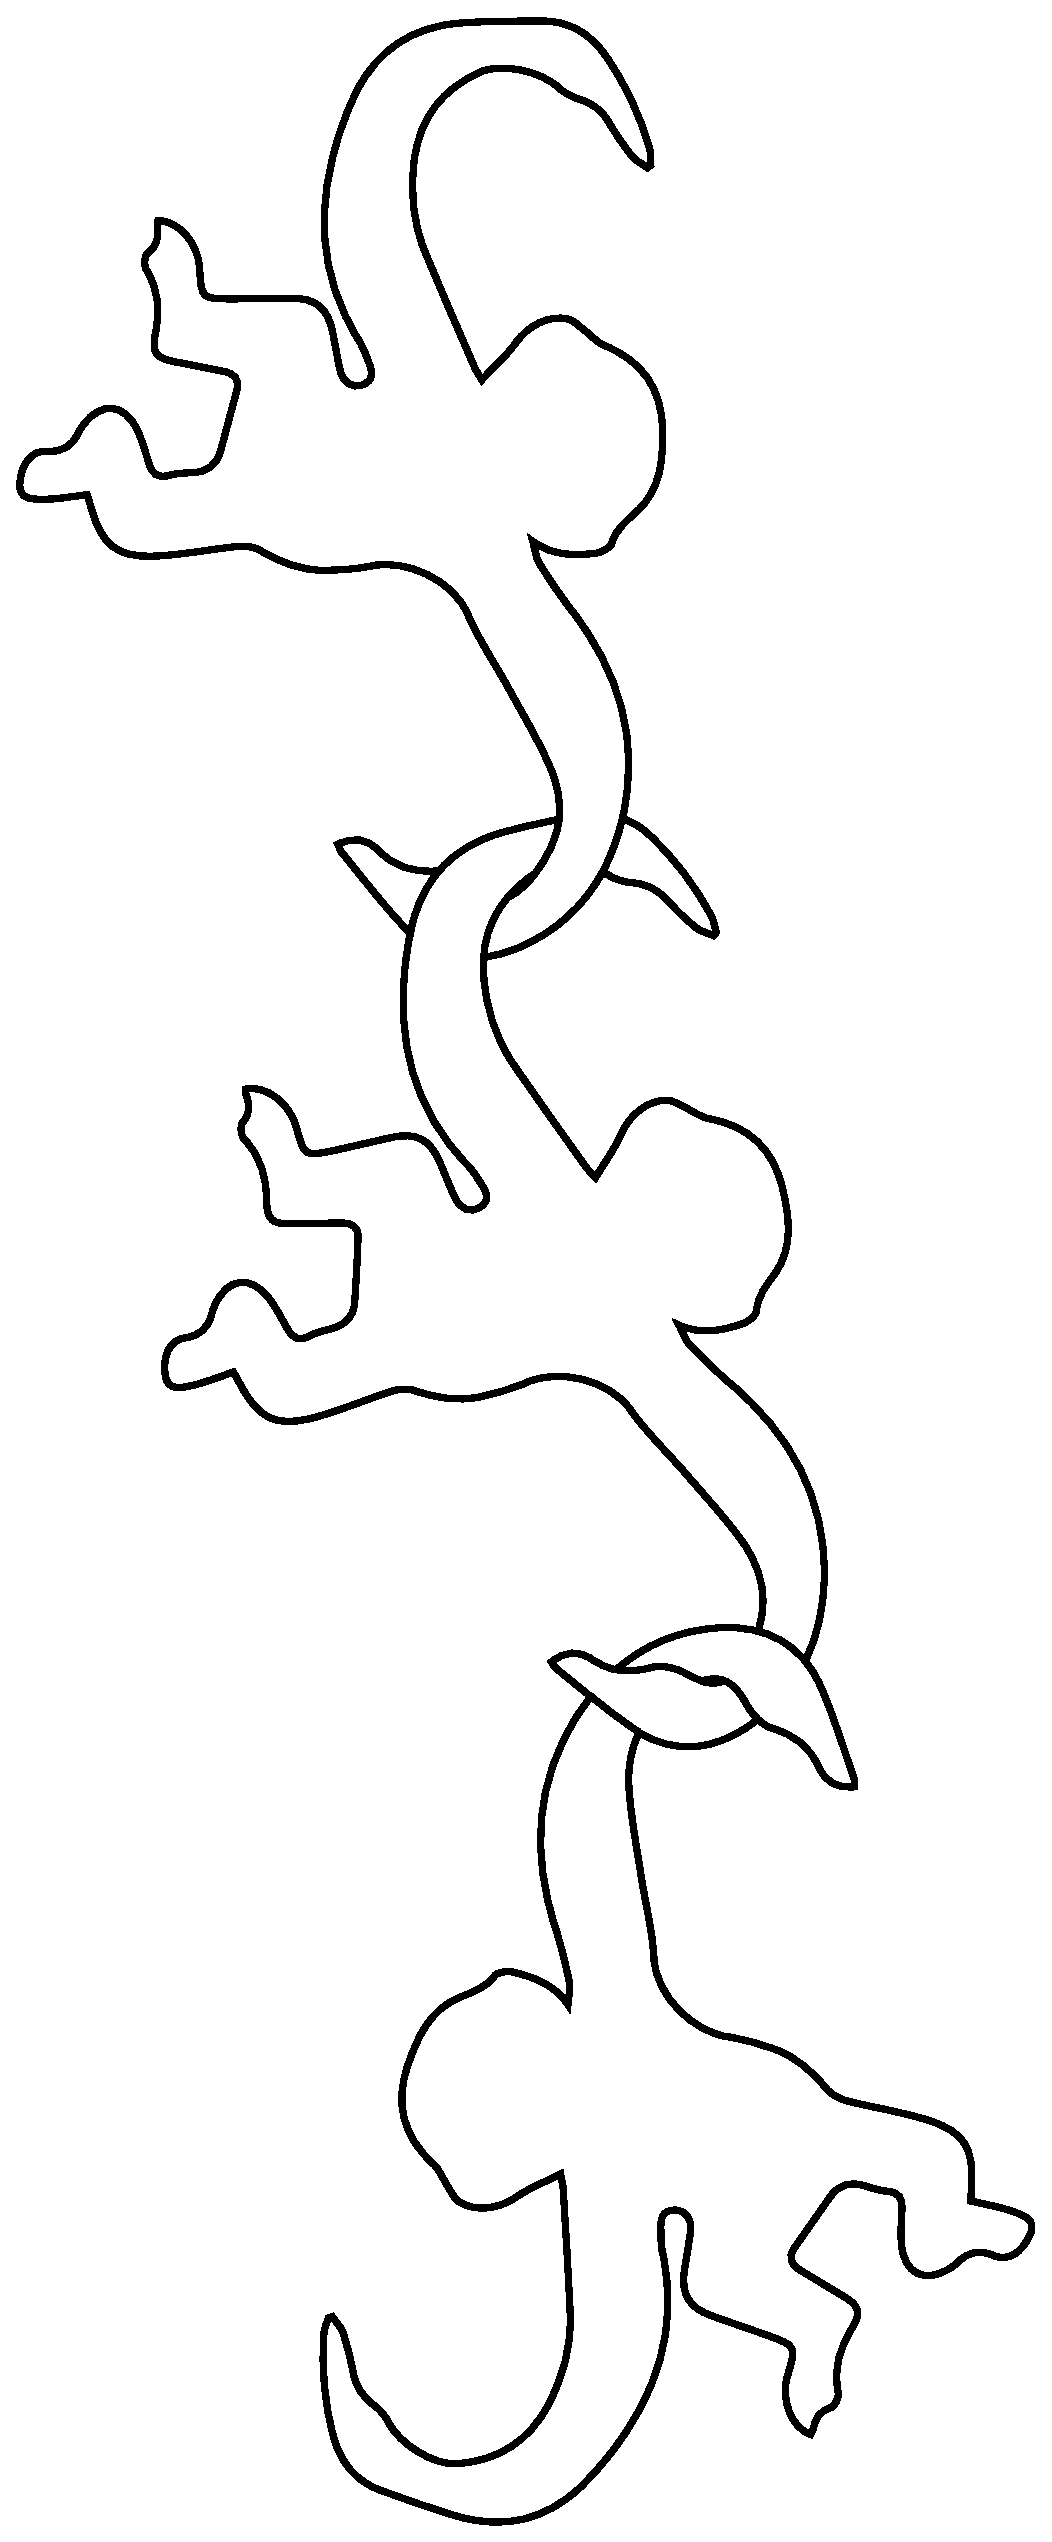
\includegraphics[width=3cm]{barrelmonkey.eps}};
		\node at (-0.25,2.4) {\scriptsize{$m=\unit[40]{g}$}};
		\node[rotate=2] at (0.12,0.1) {\scriptsize{$m=\unit[30]{g}$}};
		\node[rotate=-20] at (0.3,-2.5) {\scriptsize{$m=\unit[20]{g}$}};
	\end{tikzpicture}
	\vspace{20pt}
	\end{center}
\end{wrapfigure}

\noindent Your little brother is playing with monkeys in a barrel. The mass of each monkey is indicated in the illustration on the right. Note that your brother is holding the monkeys still and his hand weighs \unit[50]{N}.

\begin{enumerate}[(a)]
	\item Make a separate \forcediag{} for each of the four objects, the hand, top monkey, middle monkey, bottom monkey.
	
	\item Identify all 3rd law pairs of forces appearing in your \forcediags{} by circling the two forces and connecting them with a line.
	
	\item Use Newton's 1st and 3rd laws to numerically determine all of the forces acting on the monkeys and the hand. If necessary, redraw your \forcediags{}, so they are more to scale.
\end{enumerate}
\end{fnt}

\vspace{-6pt}
\WCD
\vspace{12pt}

%\section{Some things to ponder before we begin}
\label{act8.1.0-part2}

\begin{fnt}
	\input{U8/fnt8.1.0-2}
\end{fnt}

\vspace{-6pt}
\WCD

%We'll skip this one...
%\begin{fnt}
%	\input{U8/fnt8.1.1-3}
%\end{fnt}

%\WCD

%\begin{fnt}
%	\input{U8/fnt8.1.1-4}
%\end{fnt}
%
%\WCD



%%%%%%%%%%%%%%%%%%%%%%%%%%%%%%%%%%%%%%%%%%%%%%%%%%%%%%%%%%%%%%%%%%%%%%%%
%
%		DLM 16C
%
%%%%%%%%%%%%%%%%%%%%%%%%%%%%%%%%%%%%%%%%%%%%%%%%%%%%%%%%%%%%%%%%%%%%%%%%

%\chapter[\chaptername\thechapter]{\chapterlongname \thechapter}
%\label{dlm16c}
%\addchapter

%	%\section{Some things to ponder before we begin}
\label{act8.1.0-part2}

\begin{fnt}
	\label{fnt8.1.0-2}

We've already investigated this problem with one spring scale in \ref{8.1.0-1}. Now, imagine you have two spring scales, A and B, connected at the end of the scale that doesn't move. The end that moves of each spring scale (where you take readings from) is attached to a string that goes over a pulley and connects to a \unit[1]{kg} mass for both spring scales A and B.

\vspace{-6pt}
\begin{center}
	\begin{tikzpicture}[thin,scale=.7, every node/.style={transform shape},background rectangle/.style={fill=white}, show background rectangle]
		%table
		\draw (2,3) rectangle (10,3.5);
		\draw (3,0) rectangle (3.25,3);
		\draw (8.75,0) rectangle (9,3);
		%pulleys
		\draw (1.5,3.62) circle (.3);
		\draw (10.5,3.62) circle (.3);
		\filldraw[fill=white,draw=black] (1.5,3.5) rectangle (2.5,3.7);
		\filldraw[fill=white,draw=black] (9.5,3.5) rectangle (10.5,3.7);
		%weights
		\draw (.8,1.5) rectangle (1.6,2) node[midway] {\unit[1]{kg}};
		\draw (10.4,1.5) rectangle (11.2,2) node[midway] {\unit[1]{kg}};
		%string
		\draw (1.2,2) -- (1.2,3.62);
		\draw (10.8,2) -- (10.8,3.62);
		\draw (1.5,3.92) -- (4.5,3.92);
		\draw (10.5,3.92) -- (7.7,3.92);
		%spring scales
		\draw (4.9,3.72) rectangle (5.9,4.12) node[midway,above=6pt,align=center] {\scriptsize{Spring}\\[-1.2ex]\scriptsize{Scale A}};
		\foreach \x in {5.1, 5.3, 5.5, 5.7}
			\draw (\x,3.8) -- (\x,4.04);
		\draw (6,3.92) circle (.1);
		\draw (4.7,3.92) ellipse (.2 and .1);
		\draw (6.3,3.72) rectangle (7.3,4.12) node[midway,above=6pt,align=center] {\scriptsize{Spring}\\[-1.2ex]\scriptsize{Scale B}};
		\foreach \x in {6.5, 6.7, 6.9, 7.1}
			\draw (\x,3.8) -- (\x,4.04);
		\draw (6.2,3.92) circle (.1);
		\draw (7.5,3.92) ellipse (.2 and .1);
	\end{tikzpicture}
\end{center}
\vspace{-24pt}

\begin{enumerate}[(a)]
	\item State what you think \emph{each} spring scale will read in this situation.
	
	\item Construct a logical argument that explains why the spring scales read what you reported in Question~(a). You should treat this as a quiz/test question and therefore use complete sentences, reference any models you think will strengthen your argument, and provide evidence to support your claim.
\end{enumerate}
\end{fnt}

\vspace{-6pt}
\WCD

%We'll skip this one...
%\begin{fnt}
%	\label{fnt8.1.1-3}

Use Newton's laws to analyze the three car train shown in the picture. Car~A is the engine and pulls Cars~B and C. Car~A has a mass of \unit[10000]{kg}, Car~B is \unit[8000]{kg}, and Car~C is \unit[5000]{kg}. The train is initially at rest but then starts to move with an acceleration of $\unitfrac[3]{m}{s^2}$ to the left.

Calculate the force of Car~B on Car~A. Answer the following questions to help you do this.

\begin{enumerate}[(a)]
	\item Draw a \forcediag{} for EACH car with the train at rest.

	\item Car~A powers up its engine and each car starts to accelerate. What provides the force for Car~C to start accelerating?

	\item Draw a \forcediag{} for each car now that each car is accelerating (You may need to come back and update them after you determine the numerical values for each force).

	\item Calculate the force of Car~B on Car~C. 
		
		\textbf{Hint:} the sum of the forces on EACH car is equal to the mass of that car times the car's acceleration. $\sum \vec{F}_A = m_A \vec{a}_A$.
	
	\item What is the net force on Car~B?
	
	\item Calculate the force of Car~A on Car~B.
	
	\item What is the force of Car~B on Car~A?
	
	\item What is the magnitude and direction of the force of the rails on Car~A?
\end{enumerate}
%\end{fnt}

%\WCD

%\begin{fnt}
%	\label{fnt8.1.1-4}

For each of the following
\begin{enumerate}[(i)]
	\item Identify all the forces acting on the object of interest (\textbf{\em bold} in each statement) in each of the situations below.
	
	\item Draw a \forcediag{} for the object of interest.
	
	Note: Be sure to label your force vectors and make their length approximately equal to their magnitudes.
\end{enumerate}

\begin{enumerate}[(a)]
	\item The \textbf{\em softball player} is slowing as she slides into the base.
	\item The \textbf{\em child} on the swing who is being pulled back before being released.
	\item A \textbf{\em skydiver} who is descending at a constant velocity.
	\item The \textbf{\em squirrel} that is sitting still on a slanted roof.
\end{enumerate}
%\end{fnt}
%
%\WCD
%	\newpage



%%%%%%%%%%%%%%%%%%%%%%%%%%%%%%%%%%%%%%%%%%%%%%%%%%%%%%%%%%%%%%%%%%%%%%%%
%
%		DLM 17A
%
%%%%%%%%%%%%%%%%%%%%%%%%%%%%%%%%%%%%%%%%%%%%%%%%%%%%%%%%%%%%%%%%%%%%%%%%

%Skipping all these next activities because they're introducing motion graphing. Since we only have a few weeks left, I'm not introducing another new topic. We'll introduce Newton's laws and then finish momentum with the 2D/3D pendulum, coming back to forces to look at that, and then finish 2D momentum at the end of the semester.
%\chapter[\chaptername\thechapter]{\chapterlongname \thechapter}
%\label{dlm17a}
%\addchapter

%	\section{Using the \FModel{} to Analyze the Motion of Dropped Objects}
\label{act8.2.1}

\textbf{Phenomenon:} Dropping a wadded up piece of paper and a flat bottomed coffee filter

\begin{enumerate}
	\item Observing the Motion. Do (a) and (b) as a group, then put up (c) and (d) on the board.
	
	\begin{enumerate}
		\item Obtain a flat-bottomed coffee filter that still has it original shape. Wad up a piece of paper until it is in the shape and size of a golf ball. Drop both simultaneously from a height of about six feet.
		
		\item Carefully observe the motion of the two objects.
		
		\item Write out a description of the motion you observed using the terminology ``velocity.''
		
		\item Sketch a velocity graph on the board (only the vertical component) for each object on the same set of velocity versus time axes.
	\end{enumerate}

\WCD

	\item Analyzing the Motion. Discuss (a), (b), and (c) as a group while working at the board.
	
	\begin{enumerate}
		\item Create \forcediags{} for both objects at two times, 
		\begin{enumerate}
			\item first at the instant each object has been released and
			\item second after each has fallen about \nicefrac{1}{4} of the way to the floor.
		\end{enumerate}
		Show the net force vector explicitly (use double lines). What does this tell you about the accelerations of these two objects as they fall? Apply Newton's 2nd law to both objects in order to determine their accelerations.
		
			\textbf{Put all of this on the board.}
		
		\item Use the accelerations you obtained in (a) along with the actual motions you observed to make an acceleration graph ($\vec{a}$ versus time) for the two dropped objects from the time they are released to just before hitting the floor.
		
			\textbf{Put these graphs on the board.}
		
		\item What is the mathematical relation between the instantaneous acceleration and the instantaneous velocity? How does this relation show up on the two graphs you made for the two cases? Adjust your curves to be consistent with both (b) and (c).
	\end{enumerate}
\end{enumerate}

\textbf{\em Be prepared to share your responses with the whole class.}

\WCD
 %part 2
%	\newpage
%	\section{The \FModel{}}
\label{act8.2.2}

\begin{fnt}
	\label{fnt8.2.1-1}

State whether the acceleration is positive, negative, or zero for each of the position functions $\vec{x}(t)$ in the position versus time graphs below. How do you know?
\end{fnt}

\begin{fnt}
	\label{fnt8.2.1-2}

For the each of the following scenarios make a position vs.\ time graph.  Directly below it draw a velocity vs.\ time graph, and beneath that draw acceleration vs.\ time. 

\begin{enumerate}[(a)]
	\item A dropped object as it is falling (before it hits the floor). 
	\item A rocket firing its engines for a certain length of time descending on Mars.
	\item A racecar during the first 10~seconds after it starts from a stop.
\end{enumerate}
\end{fnt}

\begin{fnt}
	\label{fnt8.2.1-3}

Beneath the appropriate column of graphs from \ref{fnt8.2.1-2}, write an equation that solves for the variable in question (see below).  Write which model you used: \FModel{}, \EnergyInteractionModel{}, the \pConsModel{}, %the \LConsModel{}, 
etc... If you introduce any new variables, clearly indicate what they mean.

\begin{enumerate}[(a)]
	\item The velocity of a dropped object just before it hits the floor. 
	\item The time it takes the dropped object in (a) to reach the floor after being dropped.
	\item The change in velocity for a spacecraft firing its rockets for a certain length of time.
	\item The speed of the racecar after the first 10~seconds.
\end{enumerate}
\end{fnt}

%\begin{fnt}
%	\label{fnt8.2.1-4}

Interpret the graph to the right as representing the velocity of an object. Rank the points in order of increasing acceleration (from most negative to most positive). Practice walking this plotted motion.
%\end{fnt}

What kinds of questions can the various models answer?

In Your Small Group discuss the following and put your responses on the board.

Your instructor will assign each group one of the following tasks:

\begin{enumerate}
	\item \textbf{Group 1:}
	\begin{enumerate}
		\item Decide on your group's answer to \ref{fnt8.2.1-1}, redraw each graph and explain next to it how you know whether the $x$-component of the acceleration is positive, negative, or zero.
		\item In each case, is the $x$-component of the velocity positive or negative?
		\item Does a negative acceleration always mean a decreasing speed? Come up with a relationship between the sign of acceleration and the change in velocity and write this on the board.
		\item Go to the boards of the groups working on \ref{fnt8.2.1-2}. Check each group's answers and graphs and assign them a ``grade'' for their work on \ref{fnt8.2.1-2}; seriously do this. Grade their graphs taking into account the initial points, the signs of the slope of the line in each graph, and how the slope of the line in each graph changes with time. Don't give them a low grade just because their answer doesn't look like your answer. Only give them a low grade if their answer is an unreasonable one for the problem at hand.
	\end{enumerate}
	
	\item \textbf{Groups 2, 3, \& 4:} For your group's assigned scenario from \ref{fnt8.2.1-2}, make a column of three graphs with the top most being position vs.\ time and the bottom most acceleration vs.\ time. Line up your graphs so that a vertical line through all three would correspond to the same instant in time in each.
	
	\item \textbf{Group 5:} Go to the boards of the groups working on \ref{fnt8.2.1-2} and answer \ref{fnt8.2.1-3} by writing the appropriate equation and naming which model is used.
	
	\item \textbf{All groups:} What kinds of questions can the \FModel{} answer that the conservation models cannot answer? Explain why. (Use what you have learned from lecture and/or the Course Notes to help you answer this question.) Give two specific examples.
\end{enumerate}

\WCD

	
	

%%%%%%%%%%%%%%%%%%%%%%%%%%%%%%%%%%%%%%%%%%%%%%%%%%%%%%%%%%%%%%%%%%%%%%%%
%
%		DLM 17B
%
%%%%%%%%%%%%%%%%%%%%%%%%%%%%%%%%%%%%%%%%%%%%%%%%%%%%%%%%%%%%%%%%%%%%%%%%

%\chapter[\chaptername\thechapter]{\chapterlongname \thechapter}
%\label{dlm17b}
%\addchapter

%	\section[Graphs of Motion and Newton's 2nd Law]{Making Sense of Motion from Graphs And Newton's 2nd Law}
\label{act8.2.3}

\begin{fnt}
	\label{fnt8.2.1-4}

Interpret the graph to the right as representing the velocity of an object. Rank the points in order of increasing acceleration (from most negative to most positive). Practice walking this plotted motion.
\end{fnt}

Discuss your group's response to the following prompts and then put your responses up on the board.
\begin{enumerate}
	\item Describe in words the motion of the object whose velocity is shown in the graph. Practice walking this graph for the whole class presentation.
	\item Explain exactly how you can determine the acceleration from a graph of velocity vs.\ time.
	\item Construct an acceleration graph from the velocity graph shown in this FNT.
	\item Describe in words how the net force on this object changes from one lettered point to the next.
\end{enumerate}

\WCD

\begin{fnt}
	\label{fnt8.2.1-5}

The velocity graph of a \unit[1]{g} coffee filter released from rest is shown below. Note the break in the time axis. Four distinct intervals are shown on the graph.
\begin{enumerate}[(a)]
	\item Speed downward increasing from rest, $\unit[0]{s} \leq t \leq \unit[0.02]{s}$.
	\item Speed downward increasing, $\unit[0.02]{s} \leq t \leq \unit[0.09]{s}$.
	\item Speed downward is constant, $\unit[0.09]{s} \leq t \leq \unit[4.99]{s}$.
	\item Landing on the floor, $\unit[4.99]{s} \leq t \leq \unit[5.00]{s}$.
\end{enumerate}
Draw an acceleration graph for the same time intervals above. You may use the tangent lines drawn on the velocity graph to calculate the average slopes of the velocity curve during the first two intervals.
\end{fnt}

Discuss how you can be sure that the values of the acceleration you determined from the velocity graph in regions (a) and (c) are the correct values according to Newton's 2nd law. Show this ``check'' on the board. Note: you do not have to put the graph on the board.

\WCD

\begin{fnt}
	\label{fnt8.2.1-6}

Refer to the graphs on the reverse which were made using a motion detector mounted above a basketball that was dropped from a height of \unit[1.5]{m} above the floor. The position measured and indicated is really the position of the top surface of the ball. The velocity graph was computed by the software as the derivative of the position vs.\ time graph. Complete the following tasks related to this situation.

\begin{enumerate}[(a)]
	\item Determine accurately the acceleration from the velocity graph and plot it on the acceleration axis. Make sure you extend the acceleration curve as far as the other two are extended in time.
	
	\item Describe the motion of the ball at the six indicated times numbered [1] to [6]. That is, describe where it is located and say something about its speed, direction of motion, and acceleration. If you look closely, you should see that at position [3] the ball is still in contact with the floor.
	
	\item Draw \forcediags{} for each of the six marked times. For which times are the \forcediags{} identical?
	
	\item For the times when the \forcediags{} are identical, which aspects of the motion are identical? Which aspects are different? Are your answers to the previous two questions consistent with Newton's 2nd law?
	
	\item Determine the average value of the force exerted by the floor on the ball between the times numbered [2] and [3] two different ways:
	\begin{enumerate}[(i)]
		\item from the impulse imparted to the ball from the floor and the velocity graph; and 
		\item using Newton's 2nd law.
	\end{enumerate}
	Explain two ways (once for each approach) why the force of the floor on the basketball when it bounces is so much greater than the basketball's weight.
\end{enumerate}
\end{fnt}

Discuss your group's responses to all parts of this FNT and respond to the following prompts.
\begin{enumerate}
	\item Put your responses to part (a) on the board.
	\item Put only the \textbf{different} \forcediags{} on the board for part (c) and note above each diagram which points, [1] through [6], it applies to. Make sure everyone in your group understands part (d) and is prepared to share with the class.
	\item Make sure everyone in your group understands part (e) and is prepared to share with the class.
\end{enumerate}

\WCD

\begin{fnt}
	\label{fnt8.2.1-7}

Consider the following ``problem'' that many beginning physics students struggle with: ``How is it that at a certain instant in time, an object can have zero velocity, but at that same instant, have a non-zero acceleration?''  Figure out how to explain this using the graphs of the motion of the dropped and bouncing basketball, the basic definitions of velocity and acceleration, and Newton's 2nd law.
\end{fnt}

Discuss this FNT in your group and put a \textbf{concise} explanation on the board.

\WCD

\begin{fnt}
	\label{fnt8.1.1-1}

\textbf{Cart and Horse Paradox:} If a horse pulls on a cart, and the cart pulls back on the horse with an equal magnitude force, how can either possibly begin to move?

Use what you have learned about force to \textbf{give a complete explanation of this paradox.} For a complete explanation, make and refer to complete \forcediags{} for each of the following.
\begin{enumerate}[(a)]
	\item the horse, 
	\item the cart, and 
	\item the whole system (horse \& cart).
\end{enumerate}
\end{fnt}

Discuss this FNT in your group, put the three \forcediags{} on the board, and make sure everyone in your group understands these and is prepared to share with the class.

\WCD
%	\newpage
%	\input{U8/cylinder-activity}
	
	

%%%%%%%%%%%%%%%%%%%%%%%%%%%%%%%%%%%%%%%%%%%%%%%%%%%%%%%%%%%%%%%%%%%%%%%%
%
%		DLM 18?
%
%%%%%%%%%%%%%%%%%%%%%%%%%%%%%%%%%%%%%%%%%%%%%%%%%%%%%%%%%%%%%%%%%%%%%%%%

%\chapter[\chaptername\thechapter]{\chapterlongname \thechapter}
%\label{dlm18}
%\addchapter

	\section{Ball Swinging in a Horizontal Circle}

\begin{overview}

	\textbf{Overview:} Remember the Mass Swinging in a Horizontal Circle in Activity \ref{MassCircle}? We already started analyzing the forces acting on the ball in that activity. Now that we have another model in our tool bag, we return to this scenario to continue our analysis of the forces on the ball.
	
\end{overview}

\noindent\textbf{Phenomenon:} Ball on a string, swinging in a horizontal circle at constant speed. The experiment shows that as the ball moves faster, $\theta$ becomes larger, and the tension in the string increases.

%\begin{wrapfigure}[6]{r}{6cm}
%        \centering
%        \vspace{-\baselineskip}
\begin{center}
			\begin{tikzpicture}{r}{1}
				% Reference Measurements
				\draw[dashed] (2,3.5) -- (2,0);
				\draw[dashed] (2,0.5) ellipse (2cm and 0.25cm);
				\draw[thin] (2,0.5) -- (4,0.5) node[midway,above=1.5pt] {$r$};
				\draw[thin] (2,2.5) arc (270:240:1) node[below=2pt] {$\theta$};
				
				% Ball & String
				\draw[thick] (2,3.5) -- (0,0.5) node[midway,left=3pt] {$\ell$};
				\draw[fill=gray] (0,0.5) circle (0.125cm);
			\end{tikzpicture}
\end{center}
%	  \end{wrapfigure}


\subsection*{What model/approach would you use?}

Suppose you are interested in how the tension in the string depends on the angle $\theta$ that the string makes with the vertical direction. Which approach do you think would help you make progress with this question: energy conservation, momentum %or angular momentum
conservation, or Newton's 2nd law?\\

\noindent Discuss in your group what information you specifically need, and which models/approaches can give you that information. Start by thinking about the specific motion and what is required to produce this motion. (Note that rotational velocity -- how fast the ball swings around the circle -- is assumed constant. What does this imply?)

\subsection*{Use the model}

Carry out the analysis using whichever approach/model you have decided on.
\begin{enumerate}
	\item Put a properly labeled \forcediag{} for the ball on the board.
	\label{act8.3.1-2a}
	
	\item Use the \forcediag{} to develop \textbf{two} mathematical relationships (one for the vertical direction and one for the horizontal direction). You will need to figure out (or remember) the direction of the acceleration of an object traveling in a circle at constant speed. The magnitude of this acceleration is $a_\text{centripetal} = \frac{v_\text{tangential}{}^2}{r}$.\\(Notice $v_\text{tangential}$ refers to the \emph{tangential} speed of the ball).
	
	\item Does the force of the string on the ball equal the force of the Earth on the ball? If not, what does?
	
\WCD
\vspace{2pt}

	\item Illustrate using vectors what happens to the tension in the string ($\vec{F}_\text{string on ball}$) when the tangential speed of the ball increases. Think about how the two relationships in \eqref{act8.3.1-2a} can both be satisfied.
	
	\item Develop a short explanation of why the angle of the string (from the vertical direction) changes when the tangential velocity is increased significantly. Check this out with the real ball and string.
\end{enumerate}

\WCD

%	\newpage
%	\input{U8/cylinder-activity}
	
	


	\label{Unit8}


%%%%%%%%%%%%%%%%%%%%%%%%%%%%%%%%%%%%%%%%%%%%%%%%%%%%%%%%%%%%%%%%%%%%%%%%
%
%		APPENDICES
%
%%%%%%%%%%%%%%%%%%%%%%%%%%%%%%%%%%%%%%%%%%%%%%%%%%%%%%%%%%%%%%%%%%%%%%%%

\cleardoublepage		% Start Appendix on right hand side of page
\appendix
%\cfoot{\thechapter-\thepage}

\pagenumbering{gobble}	% No page numbers
\part*{Appendix}
\addcontentsline{toc}{part}{Appendix}

\fancyhead[LE,RO]{\sc\nouppercase{\leftmark}}
\fancyhead[RE,LO]{\sc\nouppercase{\rightmark}}

\numberwithin{page}{chapter}	% resets page number every chapter
\renewcommand{\thepage}{\thechapter-\arabic{page}}
\newcommand{\appendixchapter}[1]{\chapter{#1}\setcounter{page}{1}}
%\pagenumbering{arabic}	% reset page numbering
%\renewcommand{\thepage}{Appendix \arabic{page}}

\appendixchapter{SI Units and Conversions}
\label{UnitsConv}

\begin{table}[h]
	\centering
	\caption{Common SI Units Relating to Energy}
	\begin{tabular}{cccc}
		\hline\hline
		SI Unit	&	Construct	&	Abbreviation	&	Expressed in base units\\
		\hline
		Joule	&	energy	&	J	&	\unitfrac{kg$\cdot$m$^2$}{s$^2$} = N$\cdot$m\\
		Watt	&	power	&	W	&	\unitfrac[]{J}{s} = \unitfrac[]{kg$\cdot$m$^2$}{s$^3$}\\
		Newton	&	force	&	N	&	\unitfrac[]{kg$\cdot$m}{s$^2$}\\
		Pascal	&	pressure	&	Pa	&	\unitfrac[]{J}{m$^3$} = \unitfrac[]{N}{m$^2$}\\
		\hline\hline
	\end{tabular}
\end{table}


\begin{table}[h]
	\centering
	\caption{Some common energy units and conversions to SI}
	\begin{tabular}{c}
		\hline\hline
		\unit[1]{kWh} = \unit[3.6]{MJ}\\
		\unit[1]{erg} = \unit[10$^{-7}$]{J}\\
		\unit[1]{cal} = \unit[4.184]{J}\\
		1 food Calorie (big ``C'' calorie) = \unit[1]{kcal} = \unit[4184]{J}\\
		\unit[1]{ft$\cdot$lb} = \unit[1.36]{N$\cdot$m}\\
		\unit[1]{eV} = \unit[$1.602\times10^{-19}$]{J}\\
		\unit[1]{BTU} = \unit[778]{ft$\cdot$lb} = \unit[252]{cal} = \unit[1054]{J}\\
		\hline\hline
	\end{tabular}
\end{table}


\begin{table}[h]
	\centering
	\caption{International System (SI) of Units (Metric)}
	\begin{tabular}{ccc}
		\hline\hline
		Meter	&	Distance/Length	&	m	\\
		Centimeter	&	Distance/Length	&	cm	\\
		Kilogram	&	mass	&	kg	\\
		Gram	&	mass	&	g	\\
		Liter	&	Volume	&	L	\\
		Second	&	Time	&	s	\\
		Celsius	&	Temperature	&	\textdegree C	\\
		Kelvin	&	Temperature	&	K	\\
		Mole	&	Amount of Substance	&	mol	\\
		\hline\hline
	\end{tabular}
\end{table}


\begin{table}
	\centering
	\caption{SI Unit Conversions}
	\begin{tabular}{>{\centering}m{2cm}>{\centering}m{2cm}m{2cm}< {\centering}}
		\hline\hline
		Derived Quantity	&	SI~Units in terms of base units	&	Alternative name for SI~Unit	\\
		\hline
		Area	&	m$^2$	&	---	\\
		Volume	&	m$^3$	&	---	\\
		Density	&	\unitfrac[]{kg}{m$^3$}	&	---	\\
		Speed/Velocity	&	\unitfrac[]{m}{s}	&	---	\\
		Acceleration	&	$\frac{\unitfrac[]{m}{s}}{\unit[]{s}}$ = \unitfrac[]{m}{s$^2$}	&	---	\\
		Momentum	&	\unitfrac{kg$\cdot$m}{s}	&	---	\\
		Force	&	\unitfrac{kg$\cdot$m}{s$^2$}	&	Newton, N	\\
		Pressure	&	\unitfrac{kg}{m$\cdot$s$^2$}	&	Pascal, Pa	\\
		Work, Energy	&	\unitfrac{kg$\cdot$m$^2$}{s$^2$}	&	Joule, J	\\
		Power	&	\unitfrac{kg$\cdot$m$^2$}{s$^3$}	&	Watt, W	\\
		\hline\hline	
	\end{tabular}
\end{table}


\begin{table}
	\centering
	\caption{Conversion Factors}
	\begin{tabular}{cccc}
		\hline\hline
		Length	&	Mass/Weight$^*$	&	Temperature	&	Volume\\
		\hline
		\unit[1]{in} = \unit[2.54]{cm}	&	\unit[1]{kg} = \unit[2.20]{lbs}	&	$\left< \text{\textdegree F}\right> = \frac{9}{5}\left< \text{\textdegree C}\right> + 32$	&	\unit[1]{L} = \unit[0.26]{gal}	\\
		\unit[1]{cm} = \unit[0.39]{in}	&	\unit[1]{lb} = \unit[0.45]{kg}	&	$\left< \text{\textdegree F}\right> = \frac{9}{5}\left< {K}\right> - 459.67$	&	\unit[1]{L} = \unit[33.81]{fl oz}	\\
		\unit[1]{m} = \unit[39.37]{in} = \unit[3.28]{ft}	&	\unit[1]{g} = \unit[0.035]{oz}	&	$\left< \text{\textdegree C}\right> = \frac{5}{9}\left(\left< \text{\textdegree F}\right> - 32\right)$	&	\unit[1]{gal} = \unit[3.79]{L}	\\
		\unit[1]{ft} = \unit[0.31]{m}	&	\unit[1]{oz} = \unit[28.35]{g}	&	$\left< \text{\textdegree C}\right> = \left< \text{K}\right> - 273.15$	&	\unit[1]{gal} = \unit[128]{fl oz}	\\
		\unit[1]{km} = \unit[0.62]{mi}	&&	$\left< \text{K}\right> = \left< \text{\textdegree C}\right> + 273.15$	&	\unit[1]{mL} = \unit[1]{cc} = \unit[1]{cm$^3$}	\\
		\unit[1]{mi} = \unit[1.61]{km}	&&	$\left< \text{K}\right> = \frac{5}{9}\left(\left< \text{\textdegree F}\right> + 459.67\right)$	&	\unit[1]{fl oz} = \unit[29.57]{mL}	\\
		&&&	\unit[1]{mL} = \unit[0.034]{fl oz}	\\
		\hline\hline
	\end{tabular}\\
	\footnotesize{$^*$~Kilograms and grams are units of mass while pounds and ounces are units of weight, which is mass under the influence of gravity. This makes them units of force. These conversions might work on the surface of the earth, but not necessarily everywhere else in the universe.}
\end{table}


\begin{sidewaystable}[h]
	\centering
	\caption{Table of Melting and Boiling Points, Heats of Melting and Vaporization, and Specific Heats of Some Common Substances (at a constant pressure of one atmosphere)}
	\label{HeatCapTab}
	\begin{tabular}{c|c|cc|cc|cc|cc}
	\hline\hline
	\multirow{3}{*}{Substance}	&	\multirow{3}{*}{Formula}	&	\multicolumn{2}{c|}{Melting/Boiling} 	&	\multicolumn{2}{c|}{Heat of}	&	\multicolumn{2}{c|}{Heat of}	&	\multicolumn{2}{c}{Specific Heat,}	\\
		&		&	\multicolumn{2}{c|}{Points}	&	\multicolumn{2}{c|}{Melting}	&	\multicolumn{2}{c|}{Vaporization}	&	\multicolumn{2}{c}{$C_P$}\\
		&		&	(K)	&	(K)	&	(\unitfrac[]{kJ}{kg})	&	(\unitfrac[]{kJ}{mol})	&	(\unitfrac[]{kJ}{kg})	&	(\unitfrac[]{kJ}{mol})	&	(\unitfrac[]{J}{K$\cdot$mol})	&	(\unitfrac[]{kJ}{kg$\cdot$K})	\\\hline
		Aluminum	&	\ce{Al(s)}	&	933	&	2600	&	389.18	&	10.5	&	10790	&	291	&	24.3	&	0.900	\\%\hline
		Bismuth	&	\ce{Bi(s)}	&	544	&	1693	&	52.2	&	10.9	&	722.5	&	151	&	25.7	&	0.123	\\\hline
		Copper	&	\ce{Cu(s)}	&	1356	&	2839	&	205	&	13	&	4726	&	300.3	&	24.5	&	0.386	\\%\hline
		Gold	&	\ce{Au(s)}	&	1336	&	3081	&	62.8	&	1.24	&	1701	&	33.5	&	25.4	&	0.126	\\\hline
		Ice (\unit[-10]{\textdegree C})	&	\ce{H2O(s)}	&&&&&&&	36.9	&	2.05	\\
		Water	&	\ce{H2O(l)}	&	273	&	373	&	333.5	&	6.01	&	2257	&	40.7	&	75.2	&	4.18	\\
		Steam	&	\ce{H2O(g)}	&&&&&&&	33.6	&	1.866	\\\hline
		Lead	&	\ce{Pb(s)}	&	600	&	2023	&	24.7	&	5.12	&	858	&	177.78	&	26.4	&	0.128	\\\hline
		Sodium	&	\ce{Na(s)}	&&&&&&&	28.2	&	1.23\\
		Sodium	&	\ce{Na(l)}	&	370.82	&	1154.4	&	114.8	&	2.64	&	4306	&	99	&	 32.7	&	1.42	\\\hline
		Silver	&	\ce{Ag(s)}	&	1234.93	&	2436	&	88.2	&	9.5	&	2323	&	250.6	&	25.4	&	0.233	\\\hline
		Mercury	&	\ce{Hg(s)}	&&&&&&&	28.3	&	0.141\\
		Mercury	&	\ce{Hg(l)}	&	234	&	5630	&	11.3	&	2.3	&	5296	&	59.1	& 28	&	0.140\\
		Mercury	&	\ce{Hg(g)}	&&&&&&&	20.8	&	0.103	\\\hline
		Tungsten	&	\ce{W(s)}	&	3410	&	5900	&	184.1	&	33.86	&	4812	&	884.85	&	24.6	&	0.134	\\%\hline
		Nitrogen	&	\ce{N2(g)}	&	63.14	&	77	&	25.7	&	0.720	&	199.1	&	5.58	&	29.04	&	1.04	\\\hline
		Oxygen	&	\ce{O2(g)}	&	54.39	&	90.18	&	13.9	&	0.444	&	213.1	&	6.82	&	29.16	&	0.911	\\\hline
		Iron	&	\ce{Fe(s)}	&	1535	&	3000	&&&&&	25.1	&	0.449	\\
		\hline\hline
	\end{tabular}
\end{sidewaystable}


\begin{sidewaystable}[h]
	\centering
	\caption{Metric Prefixes}
	\begin{tabular}{ccccc}
	\hline
	Prefix	&	Symbol	&	$10^n$	&	Decimal	&	English word	\\
	\hline\hline
	yotta	&	Y	&	 $10^{24}$	&	$1 \; 000 \; 000 \; 000 \; 000 \; 000 \; 000 \; 000 \; 000$\phantom{$1 \; 000 \; 000 \; 000 \; 000 \; 000 \; 000 \; 000 \; 00$}	&	septillion	\\
	zetta	&	Z	&	 $10^{21}$	&	$1 \; 000 \; 000 \; 000 \; 000 \; 000 \; 000 \; 000$\phantom{$1 \; 000 \; 000 \; 000 \; 000 \; 000 \; 000 \; 00$}	&	sextillion	\\
	exa	&	E	&	 $10^{18}$	&	$1 \; 000 \; 000 \; 000 \; 000 \; 000 \; 000$\phantom{$1 \; 000 \; 000 \; 000 \; 000 \; 000 \; 00$}	&	quintillion	\\
	peta	&	P	&	 $10^{15}$	&	$1 \; 000 \; 000 \; 000 \; 000 \; 000$\phantom{$1 \; 000 \; 000 \; 000 \; 000 \; 00$}	&	quadrillion	\\
	tera	&	T	&	 $10^{12}$	&	$1 \; 000 \; 000 \; 000 \; 000$\phantom{$1 \; 000 \; 000 \; 000 \; 00$}	&	trillion	\\
	giga	&	G	&	 $10^9$	&	$1 \; 000 \; 000 \; 000$\phantom{$1 \; 000 \; 000 \; 00$}	&	billion	\\
	mega	&	M	&	$10^6$	&	$1 \; 000 \; 000$\phantom{$1 \; 000 \; 00$}	&	million	\\
	kilo	&	k	&	$10^3$	&	$1 \; 000$\phantom{$1 \; 00$}	&	thousand	\\
	hecto	&	h	&	$10^2$	&	100\phantom{10}	&	hundred	\\
	deca	&	da	&	$10^1$	&	10\phantom{1}	&	ten	\\
	---	&	---	&	$10^0$	&	1	&	one	\\
	deci	&	d	&	$10^{-1}$	&	\phantom{1.}0.1	&	tenth	\\
	centi	&	c	&	$10^{-2}$	&	\phantom{01.}0.01	&	hundredth	\\
	milli	&	m	&	$10^{-3}$	&	\phantom{001.}0.001	&	thousandth	\\
	micro	&	$\mu$	&	$10^{-6}$	&	\phantom{00000\;1.}$0.000 \; 001$	&	millionth	\\
	nano	&	n	&	$10^{-9}$	&	\phantom{000\;000\;001.}$0.000 \; 000 \; 001$	&	billionth	\\
	pico	&	p	&	$10^{-12}$	&	\phantom{000\;000\;000\;001.}$0.000 \; 000 \; 000 \; 001$	&	trillionth	\\
	femto	&	f	&	$10^{-15}$	&	\phantom{000\;000\;000\;000\;001.}$0.000 \; 000 \; 000 \; 000 \; 001$	&	quadrillionth	\\
	atto	&	a	&	$10^{-18}$	&	\phantom{000\;000\;000\;000\;000\;001.}$0.000 \; 000 \; 000 \; 000 \; 000 \; 001$	&	quintillionth	\\
	zepto	&	z	&	$10^{-21}$	&	\phantom{000\;000\;000\;000\;000\;000\;001.}$0.000 \; 000 \; 000 \; 000 \; 000 \; 000 \; 001$	&	sextillionth	\\
	yocto	&	y	&	$10^{-24}$	&	\phantom{000\;000\;000\;000\;000\;000\;000\;001.}$0.000 \; 000 \; 000 \; 000 \; 000 \; 000 \; 000 \; 001$	&	septillionth	\\
	\hline
	\end{tabular}
\end{sidewaystable}
\appendixchapter{\ThreePhaseModel{}}

\subsection*{Graphical Representation}

\begin{center}
\begin{tikzpicture}
	% title the diagram
	 \draw (7.5,7) node[align=center] {\textbf{\TempGraph{}}};

    % draw horizontal axis
    \draw[-{Stealth[scale=1.2]}, line width=1pt] (0,0) -- (14.5,0);
    % label the horizontal axis
    \draw (7.5,0) node[below=3pt] {Energy Added or Removed $\Delta E$ (at constant pressure)};

    % draw vertical axis
     \draw[-{Stealth[scale=1.2]}, line width=1pt] (0,0) -- (0,7);
    % label the vertical axis
     \draw (0,7.2) node[left=10pt, rotate=90] {Temperature $T$};
    % add melting point and boiling point on axis
     \draw[line width=1pt] (-3pt,1.8 cm) -- (3pt,1.8 cm) node[left=3pt] {\scriptsize{$T_\text{MP}$}};
     \draw[line width=1pt] (-3pt,3.8 cm) -- (3pt,3.8 cm) node[left=3pt] {\scriptsize{$T_\text{BP}$}};

	% draw first segment
	 \draw[line width=.8pt,dashed] (0,0) -- (1.5,1.8) node[below left=10pt, rotate=50.19442891] {\tiny{solid phase}};
	 
	% draw second segment
	 \draw[line width=.8pt,dashed] (1.5,1.8) -- (6,1.8) node[below left] {\tiny{mixed phase: solid/liquid}};
	 
	% draw third segment
	 \draw[line width=.8pt,dashed] (6,1.8) -- (8,3.8) node[below left=10pt, rotate=45] {\tiny{liquid phase}};

	% draw fourth segment
	 \draw[line width=.8pt,dashed] (8,3.8) -- (11.5,3.8) node[below left] {\tiny{mixed phase: liquid/gas}};

	% draw fifth segment
	 \draw[line width=.8pt,dashed] (11.5,3.8) -- (14,6.5) node[below left=10pt, rotate=47.20259816] {\tiny{gas phase}};
	 
	% draw labels
	 \draw[{Stealth[scale=1]}-] (1.5,1.8) -- (1,2.8) node[above,align=center] {\tiny{All solid at $T_\text{MP}$}};
	 \draw[{Stealth[scale=1]}-] (6,1.8) -- (5.5,2.8) node[above,align=center] {\tiny{All liquid at $T_\text{MP}$}};
	 \draw[{Stealth[scale=1]}-] (8,3.8) -- (7.5,4.8) node[above,align=center] {\tiny{All liquid at $T_\text{BP}$}};
	 \draw[{Stealth[scale=1]}-] (11.5,3.8) -- (11,4.8) node[above,align=center] {\tiny{All gas at $T_\text{BP}$}};
\end{tikzpicture}
\end{center}

\subsection*{Algebraic Representations}

\noindent Change in temperature $\Delta T$ of an amount $m$ of a substance with specific heat $C_p$ when energy is \emph{added} or \emph{removed} as \emph{heat} $Q$:
\begin{align*}
	\Delta T = \frac{Q}{C_p \cdot m}
\end{align*}

\noindent Amount $\Delta m$ of a substance with heat of melting/vaporization/sublimation $\Delta H$ that changes phase when energy is \emph{added} or \emph{removed} as \emph{heat} $Q$:
\begin{align*}
	\left|\Delta m\right| = \frac{Q}{H_p}
\end{align*}


\pagebreak


\newcommand{\leftcolumn}{0.35\linewidth}
\newcommand{\rightcolumn}{0.65\linewidth}

\noindent
\parbox[b]{\leftcolumn}{
	\textbf{Constructs}}
\parbox[b]{\rightcolumn}{
	\textbf{Relationships}}

\noindent
\hrulefill

\noindent
\begin{minipage}[c]{\leftcolumn}
	\baselineskip=1.5\baselineskip
	Pure Substances\\
	Three \emph{Phases}: \emph{solid}, \emph{liquid}, \emph{gas}\\
	Temperature\\
	Energy \emph{transferred} as\\
	\hspace*{5mm}\emph{Heat} or \emph{Work}
\end{minipage}
\begin{minipage}[c]{\rightcolumn}
	\begin{enumerate}
		\item {\em Pure substances} exist in one of three phases, depending on the \emph{temperature} and \emph{pressure}: solid, liquid, and gas. {\em Non}-pure substances, e.g., solutions and composites, require more complex models for analysis.
		\item To change either the \emph{temperature} or the \emph{phase} of a substance, \emph{energy} must be \emph{added} or \emph{removed}. Often, this energy is \emph{transferred} to or from the substance as \emph{heat} $Q$ but can also be transferred as \emph{work} $W$.\\[0.2mm]
	\end{enumerate}
\end{minipage}

\noindent
\begin{minipage}[c]{\leftcolumn}
	\baselineskip=1.5\baselineskip
	Phase Change Temperatures:\\
	\hspace*{5mm}$T_\text{MP}$, $T_\text{BP}$, $T_\text{SP}$\\
	\emph{Melting}, \emph{Boiling}, \emph{Sublimation}
\end{minipage}
\begin{minipage}[c]{\rightcolumn}
\begin{enumerate}\setcounter{enumi}{2}
	\item At constant pressure, changes of {\em phase} (solid~$\Leftrightarrow$~liquid and liquid~$\Leftrightarrow$~gas, or at some values of pressure, solid~$\Leftrightarrow$~gas) occur at specific temperatures: the \emph{phase change temperatures} $T_\text{MP}$, $T_\text{BP}$, and $T_\text{SP}$. They have particular values for each pure substance. The values of these temperatures are the same when ``going through'' the respective phase change in ``both directions.'' However, phase change temperatures are \emph{dependent on the pressure}.\\[0.2mm]
	\end{enumerate}
\end{minipage}

\noindent
\begin{minipage}[c]{\leftcolumn}
	\baselineskip=1.2\baselineskip
	Heat of \emph{Melting}\\
	Heat of \emph{Vaporization} (Boiling)\\
	Heat of \emph{Sublimation}\\[0.1mm]
\end{minipage}
\begin{minipage}[c]{\rightcolumn}
	\begin{enumerate}
		\item[] The amount of \emph{energy added} or \emph{removed} during a particular \emph{phase change} (written as $\Delta H$, indicating constant pressure) is unique to each substance and has been measured and tabulated for most substances.\\[0.2mm]
	\end{enumerate}
\end{minipage}

\noindent
\begin{minipage}[c]{\leftcolumn}
	\baselineskip=1.5\baselineskip
	Thermal Equilibrium\\
	Mixed phase
\end{minipage}
\begin{minipage}[c]{\rightcolumn}
	\begin{enumerate}
		\item[] If the substance is in \emph{thermal equilibrium} (i.e., if the entire substance is at the same temperature) at the \emph{phase change temperature}, both phases will \emph{remain} at the phase change temperature as the phase change occurs. \emph{Mixed phases} can exist in thermal equilibrium {\em only} when the temperature has the value of the phase-change temperature.\\[0.2mm]
	\end{enumerate}
\end{minipage}

\noindent
\begin{minipage}[c]{\leftcolumn}
	\baselineskip=1.5\baselineskip
	Heat Capacity\\
	Specific Heat
\end{minipage}
\begin{minipage}[c]{\rightcolumn}
	\begin{enumerate}\setcounter{enumi}{3}
		\item Changes of {\em temperature} of a substance occur when energy is added or removed while the substance is \emph{not} at a phase-change temperature.

		When the energy added is in the form of heat, the change in temperature $\Delta T$ is related to the amount of energy added by a property of the substance called \emph{heat capacity} $C$. The \emph{specific heat} $C_p$ (heat capacity per unit mass) has a particular value for each substance. This value has been measured and tabulated for most substances (see Table \ref{HeatCapTab} in Appendix \ref{UnitsConv}).
	\end{enumerate}
\end{minipage}
\appendixchapter{\EnergyInteractionModel{}}

\subsection*{Graphical Representation: The \EnergyDiagram{}}

Generic Example involving two physical systems, three energy systems, and with energy added to the system as heat. The \textbf{physical system} consists of \emph{physical thing 1} and \emph{physical thing 2}.

\begin{center}
%	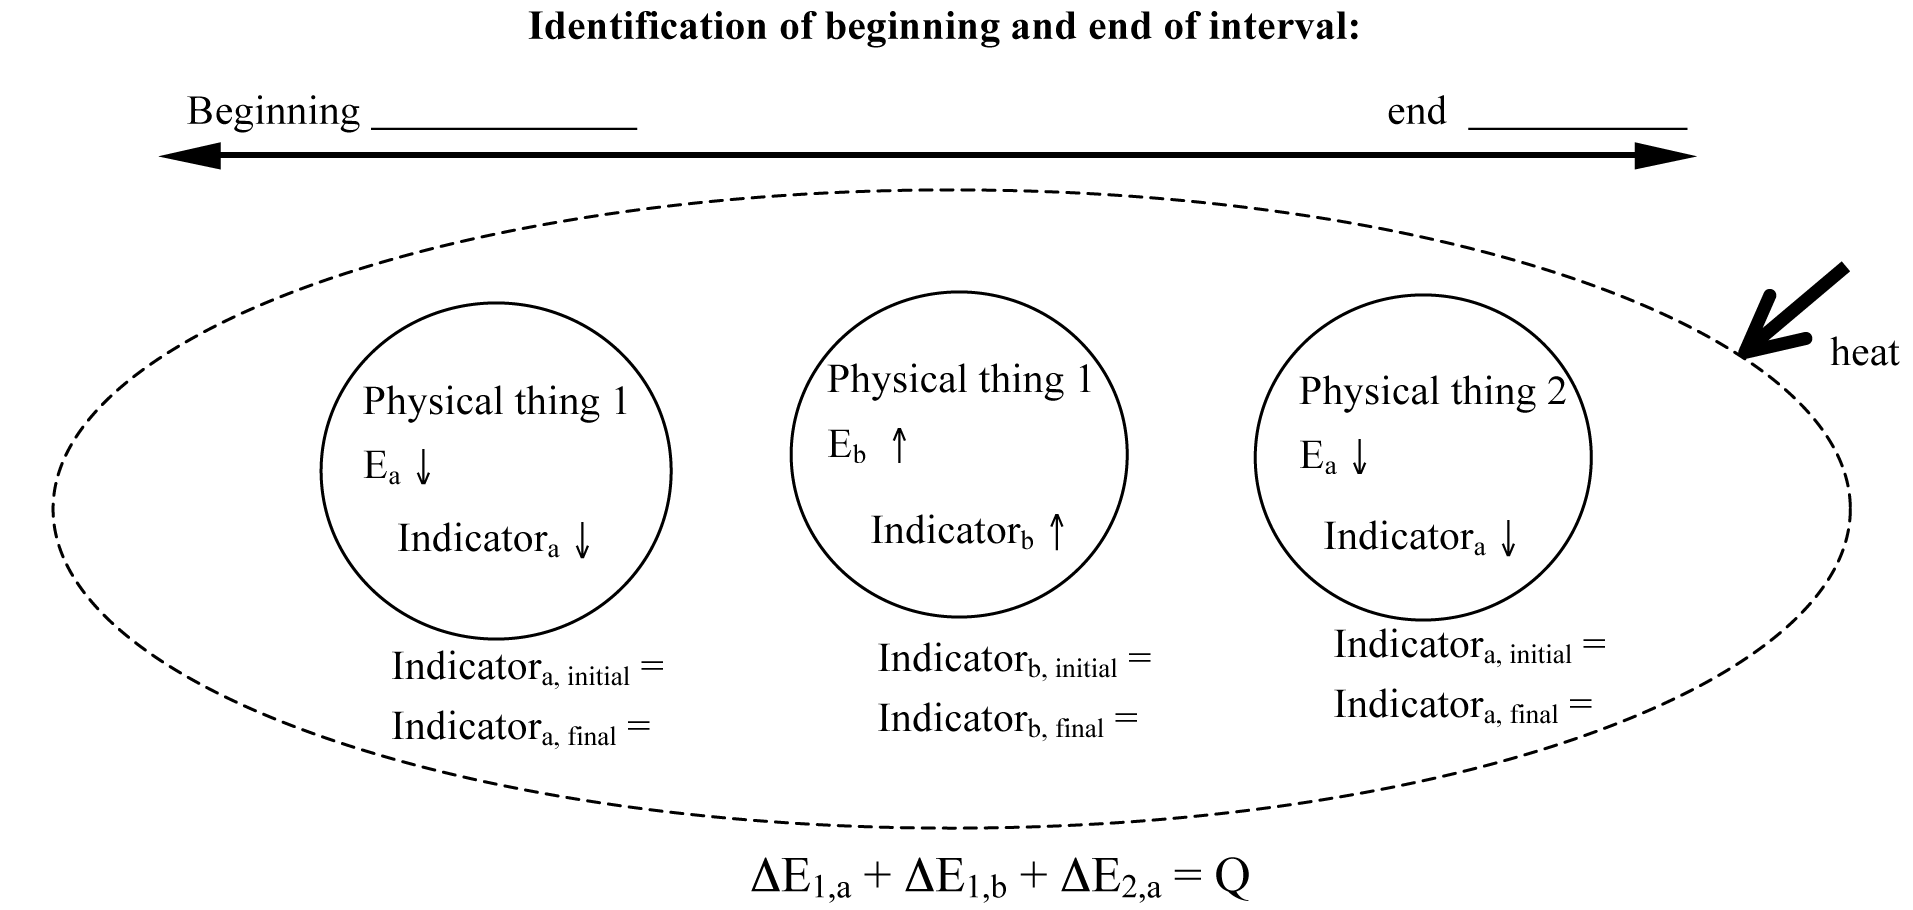
\includegraphics[width=0.8\linewidth]{E-ID}
	
\begin{tikzpicture}
    % draw horizontal line   
    \draw[-{Stealth[scale=1.2]}, line width=1pt] (0,0) -- (10.2,0);

    % draw vertical lines
    \foreach \x in {0.5,9.5}
      \draw[line width=1pt] (\x cm,3pt) -- (\x cm,-3pt);

    % title the diagram
    \draw (5,0) node[above=18pt] {\scriptsize{\textbf{Identification of \emph{beginning} and \emph{end} of interval:}}};

    % draw nodes along the interval timeline
    \draw (0.5,0) node[below=3pt] {\scriptsize{initial conditions}} node[above=3pt] {\emph{beginning}};
    \draw (9.5,0) node[below=3pt] {\scriptsize{final conditions}} node[above=3pt] {\emph{end}};

    % draw the physical system boundary
    \draw [dashed,orange,line width=1pt] (5,-2.75) ellipse (6cm and 2.25cm) node[above=1.5cm] {\textbf{\emph{physical system}}};
    
    % draw energy systems
    \draw (2,-3) node[draw,circle,blue,minimum size=2.25cm,inner sep=0pt,align=center]  {\color{darkgray}\tiny{indicator $a$}\\[.5ex]$\downarrow E_\text{1,a}$\\\color{darkgray}\tiny{$a_i =$}\\[-1.2ex]\color{darkgray}\tiny{$a_f =$}} node[orange,above=1.1cm] {\scriptsize{physical thing 1}};
    \draw (5,-3.25) node[draw,circle,blue,minimum size=2.25cm,inner sep=0pt,align=center]  {\color{darkgray}\tiny{indicator $b$}\\[.5ex]$\uparrow E_\text{1,b}$\\\color{darkgray}\tiny{$b_i =$}\\[-1.2ex]\color{darkgray}\tiny{$a_f =$}} node[orange,above=1.1cm] {\scriptsize{physical thing 1}};
    \draw (8,-3) node[draw,circle,blue,minimum size=2.25cm,inner sep=0pt,align=center]  {\color{darkgray}\tiny{indicator $a$}\\[.5ex]$\downarrow E_\text{2,a}$\\\color{darkgray}\tiny{$a_i =$}\\[-1.2ex]\color{darkgray}\tiny{$a_f =$}} node[orange,above=1.1cm] {\scriptsize{physical thing 2}};    

    % draw heat arrow
    \draw[{Stealth[scale=1.2]}-, line width=1pt, blue] (10,-2.25) -- (11,-1.5)  node[right=0cm] {heat Q};
    
    % write energy conservation equation
    \draw (5,-6) node[] {$\Delta E_\text{1,a} + \Delta E_\text{1,b} + \Delta E_\text{2,a} = Q$};
    \draw (3,-6) node[above=6pt] {\scriptsize{$(-)$}};
    \draw (4.6,-6) node[above=6pt] {\scriptsize{$(+)$}};
    \draw (6.15,-6) node[above=6pt] {\scriptsize{$(-)$}};
    \draw (7.35,-6) node[above=6pt] {\scriptsize{$(+)$}};

\end{tikzpicture}
\end{center}

\subsection*{Algebraic Representations}

\begin{align*}
	\text{Open system:} && \Delta E_\text{total} &= \sum \Delta E_i = \Delta E_1 + \Delta E_2 + \Delta E_3 + \ldots = Q + W \\[5mm]
	\text{Closed system:} && \Delta E_\text{total} &= \sum \Delta E_i = \Delta E_1 + \Delta E_2 + \Delta E_3 + \ldots = 0 \\[5mm]
	\text{Power:} && P &= \frac{\Delta E}{\Delta t}\\[5mm]
%	\text{Work:} && W &= F_\text{parallel} \Delta x = F_{||}\Delta x
\end{align*}

\pagebreak

\renewcommand{\leftcolumn}{0.375\linewidth}
\renewcommand{\rightcolumn}{0.625\linewidth}

\noindent
\parbox[b]{\leftcolumn}{
	\textbf{Constructs}}
\parbox[b]{\rightcolumn}{
	\textbf{Relationships}}

\vspace*{-\parskip}
\noindent
\hrulefill

\vspace*{-\parskip}
\noindent
\parbox[c]{\leftcolumn}{
	\noindent
	Energy
		\\\hspace*{1em}$\bullet$ Conservation of Energy
		\\\hspace*{1em}$\bullet$ Internal Energy ($U$)
		\\\hspace*{1em}$\bullet$ Mechanical Energy
		\\\hspace*{1em}$\bullet$ Energy Transfers ($Q$, $W$)\\

	\noindent
	Physical System
		\\\hspace*{1em}$\bullet$ closed
		\\\hspace*{1em}$\bullet$ open\\
	(with respect to energy transfers)\\

	\noindent
	Energy Transfer
		\\\hspace*{1em}$\bullet$ Heat, $Q$
		\\\hspace*{1em}$\bullet$ Work, $W$\\
	
	\noindent
	Energy System
		\\\hspace*{1em}$\bullet$ Indicators
		\\\hspace*{1em}$\bullet$ Change in Energy ($\Delta E$)\\
			
	\noindent
	Process or Interaction
		\\\hspace*{1em}$\bullet$ Interval
		\\\hspace*{1em}$\bullet$ initial (start) Time of Interval
		\\\hspace*{1em}$\bullet$ final (end) Time of Interval\\
	
	\noindent
	State of a Physical System
		\\\hspace*{1em}$\bullet$ Temperature
		\\\hspace*{1em}$\bullet$ Phase\\
	
	\noindent
	Energy Systems related to Thermal \& Chemical Processes
		\\\hspace*{1em}$\bullet$ $E_\text{thermal}$
		\\\hspace*{1em}$\bullet$ $E_\text{bond}$\\
	
	\noindent
	Energy Systems related to Mechanical Processes
		\\\hspace*{1em}$\bullet$ $PE_\text{gravitational}$
		\\\hspace*{1em}$\bullet$ $PE_\text{elastic}$
		\\\hspace*{1em}$\bullet$ $PE_\text{mass-spring}$
		\\\hspace*{1em}$\bullet$ $KE_\text{translational}$
		\\\hspace*{1em}$\bullet$ $KE_\text{rotational}$
	}
\parbox[c]{\rightcolumn}{
	\begin{enumerate}
		\item The heart of the \EnergyInteractionModel{} is \emph{energy conservation}, one of a few powerful \emph{conservation principles} used throughout science. One way of expressing a conservation principle is that for an isolated physical system, there are certain physical properties that do not change during an interaction or process. A process or interaction is determined by explicitly expressing the beginning and ending times of the interval characterizing the process.
		
		\item The \emph{total energy} of every \emph{physical system} can be expressed as a \emph{sum of the energies} of separately identifiable \emph{energy systems}. This division of the total energy into energy systems can be carried out in multiple ways. The energy associated with a particular energy system can be expressed in terms of \emph{observable} and \emph{measurable properties} of the physical system that we call \emph{indicators}. The \emph{change} in energy of each energy system can be determined from the \emph{observed change in the indicator} that occurs from the beginning to the end of the interval characterizing the interaction or process.
		
		\item Conservation of energy in a \emph{\textbf{closed} physical system} (isolated with respect to energy transfers from other physical systems): The \textbf{total energy} of the physical system must remain \textbf{constant} during the interaction or process. When internal interactions occur, this conservation principle can be expressed in terms of changes within the energy systems of the physical system: The \textbf{changes of the energies of \emph{all energy systems}} associated with the \emph{physical system} in question must \textbf{sum to zero}.
		
		\item Conservation of energy in an \emph{\textbf{open} physical system}: During an interaction or process during which \emph{energy is added or removed} from the physical system as heat or work, the \textbf{changes in energy of {\em all energy systems}} associated with the physical system in question must \textbf{sum to the net energy added (or removed)} as heat and/or work. Equivalently, the \textbf{change in the {\em total energy}} of that physical system must \textbf{equal the net energy added (or removed)} as heat and/or work.
	\end{enumerate}
}
	
\pagebreak

\subsection*{Steps Involved in Using the \EnergyDiagram{}}

\subsubsection*{Prior to writing anything down:}

\begin{benumerate}
	\bitem{Tell a story about what happened!} Be sure you are clear about what the physical phenomenon or process is.
\end{benumerate}

\subsubsection*{Go back and forth through Steps~2-6 until your \EnergyDiagram{} is complete:}

\begin{benumerate}\setcounter{enumi}{1}
	\bitem{What is the boundary of the physical system you are modeling?} What is inside and what is outside?
	\bitem{Is the physical system in your particular model open or closed?} If open, are there any energy transfers (e.g., heat or work)?
	\bitem{What is the extent of the process or interaction?} What determines the beginning and end?
	\bitem{What energy systems do you include in your diagram?} Which indicators are changing?
	\bitem{What are the values of the indicators at the times corresponding to the ends of the time interval you chose in step 4?}
\end{benumerate}

\subsubsection*{Only \emph{after the diagram is complete}, move on to Step~7:}

\begin{benumerate}\setcounter{enumi}{6}
	\bitem{Write down an equation expressing energy conservation for your particular \EnergyDiagram{}, in terms of the $\Delta E$'s and any $Q$ or $W$.} Each term in your conservation of energy equation must correspond to an energy system in your diagram.
\end{benumerate}

\pagebreak

\subsection*{Energy Systems and their Indicators}

\subsubsection*{Energy Systems related to \emph{Thermal \& Chemical Processes}}

\begin{tikzpicture}
	\node[draw,circle,minimum size=2.9cm,blue,inner sep=0pt, align=center] {\color{darkgray}\tiny{temperature $T$}\\[-1.2ex]\color{darkgray}\tiny{of substance}\\[.5ex]$E_\text{thermal}$\\\color{darkgray}\tiny{$\Delta T = T_f - T_i$}\\[-1.5ex]\hspace{0pt}};
	\node[align=left] at (3.8,0) {$\Delta E_\text{thermal} = m c_p \Delta T$\\\scriptsize{$m$: mass of substance}\\[-1.2ex]\scriptsize{$c_p$: Specific Heat of substance}};
\end{tikzpicture}\\

\noindent
\begin{tikzpicture}
	\node[draw,circle,minimum size=2.9cm,blue,inner sep=0pt, align=center] {\color{darkgray}\tiny{mass $m$}\\[-1.2ex]\color{darkgray}\tiny{of higher phase}\\[.5ex]$E_\text{bond}$\\\color{darkgray}\tiny{$\Delta m = m_f - m_i$}\\[-1.5ex]\hspace{0pt}};
	\node[align=left] at (3.8,0) {$\Delta E_\text{bond} = \pm | \Delta m \Delta H |$\\\scriptsize{$\Delta H$: Heat of $\langle$Phase Change$\rangle$}};
\end{tikzpicture}

\subsubsection*{Energy Systems related to \emph{Mechanical Processes}}

% first column
\begin{minipage}[c]{0.5\textwidth}

\begin{tikzpicture}
	\node[draw,circle,minimum size=2.9cm,blue,inner sep=0pt, align=center] {\color{darkgray}\tiny{height $y$}\\[-1.2ex]\color{darkgray}\tiny{above y=0}\\[.5ex]$PE_\text{gravitational}$\\\color{darkgray}\tiny{$\Delta y = y_f - y_i$}\\[-1.5ex]\hspace{0pt}};
	\node[align=left] at (4.1,0) {$\Delta PE_\text{gravitational} = m g \Delta y$\\\scriptsize{$m$: mass of object}\\[-1.2ex]\scriptsize{$g$: gravitational constant, \unitfrac[9.8]{m}{s}}};
\end{tikzpicture}\\

\noindent
\begin{tikzpicture}
	\node[draw,circle,minimum size=2.9cm,blue,inner sep=0pt,align=center] {\color{darkgray}\tiny{distance $x$}\\[-1.2ex]\color{darkgray}\tiny{from equilibrium}\\[.5ex]$PE_\text{elastic}$\\\color{darkgray}\tiny{$\Delta x^2 = x_f^2 - x_i^2$}\\[-1.5ex]\hspace{0pt}};
	\node[align=left] at (3.7,0) {$\Delta PE_\text{elastic} = \frac{1}{2} k \Delta x^2$\\\scriptsize{$k$: spring constant}};
\end{tikzpicture}\\

\noindent
\begin{tikzpicture}
	\node[draw,circle,minimum size=2.9cm,blue,inner sep=0pt,align=center] {\color{darkgray}\tiny{distance $x$}\\[-1.2ex]\color{darkgray}\tiny{from equilibrium}\\[.5ex]$PE_\text{spring-mass}$\\\color{darkgray}\tiny{$\Delta x^2 = x_f^2 - x_i^2$}\\[-1.5ex]\hspace{0pt}};
	\node[align=left] at (4.1,0) {$\Delta PE_\text{spring-mass} = \frac{1}{2} k \Delta x^2$\\\scriptsize{$k$: spring constant}\\\scriptsize{\textbf{Note} that the mass of the object}\\[-1.2ex]\scriptsize{hanging on the spring determines}\\[-1.2ex]\scriptsize{the equilibrium position!}};
\end{tikzpicture}\\
\end{minipage}
%second column
\begin{minipage}[c]{0.5\textwidth}

\noindent
\begin{tikzpicture}
	\node[draw,circle,minimum size=2.9cm,blue,inner sep=0pt,align=center] {\color{darkgray}\tiny{translational}\\[-1.2ex]\color{darkgray}\tiny{speed $v$}\\[.5ex]$KE_\text{translation}$\\\color{darkgray}\tiny{$\Delta v^2 = v_f^2 - v_i^2$}\\[-1.5ex]\hspace{0pt}};
	\node[align=left] at (4,0) {$\Delta KE_\text{translation} = \frac{1}{2} m \Delta v^2$\\\scriptsize{$m$: mass of object}};
\end{tikzpicture}\\

\noindent
\begin{tikzpicture}
	\node[draw,circle,minimum size=2.9cm,blue,inner sep=0pt, align=center] {\color{darkgray}\tiny{rotational/angular}\\[-1.2ex]\color{darkgray}\tiny{speed $\omega$}\\[.5ex]$KE_\text{rotation}$\\\color{darkgray}\tiny{$\Delta \omega^2 = \omega_f^2 - \omega_i^2$}\\[-1.5ex]\hspace{0pt}};
	\node[align=left] at (3.8,0) {$\Delta KE_\text{rotation} = \frac{1}{2} I \Delta \omega^2$\\\scriptsize{$I$: Moment of Inertia of object}};
\end{tikzpicture}
\end{minipage}

\null
\appendixchapter{Energy in Mechanical Systems}

\subsection*{Graphical Representation: The \emph{Point-to-Point Diagram}}

\textbf{Example:} A mass hanging on a spring. The total energy of the system consists of translational kinetic energy and spring-mass potential energy.

\begin{center}
\begin{tikzpicture}[thick,scale=0.8, every node/.style={transform shape}]
    % draw horizontal axis
    \draw[-{Stealth[scale=1.2]}, line width=1pt] (-5,0) -- (5,0);
    % label the horizontal axis
    \draw (0,0) node[below=3pt] {Displacement $x$ from Equilibrium};
    \draw (-4.5,0) node[below=3pt] {\scriptsize{$-x$}};
    \draw (4.5,0) node[below=3pt] {\scriptsize{$+x$}};

    % draw vertical axis
     \draw[-{Stealth[scale=1.2]}, line width=1pt] (0,0) -- (0,7);
    % label the vertical axis
     \draw (0,6.9) node[left=9pt, rotate=90] {Energy $E$};

    % draw Total Energy line
    \draw [ForestGreen,line width=1pt] (-5,4.5) -- (5,4.5);
    \draw (-3.6,4.8) node[ForestGreen] {$E_\text{total} = KE_\text{translational} + PE_\text{spring-mass}$};
    
    % draw Potential Energy line
     \draw[scale=1.12,domain=-4:4,smooth,variable=\x,blue, line width=1pt] plot ({\x},{1/2*1/2*\x*\x});
     \draw (5.5, 4) node[blue] {$PE_\text{spring-mass}$};
     
    % draw Kinetic Energy line
     \draw[scale=1.12,domain=-4:4,smooth,variable=\x,red, line width=1pt] plot ({\x},{4-(1/2*1/2*\x*\x)});
     \draw (5.6, .5) node[red] {$KE_\text{translational}$};
\end{tikzpicture}
\end{center}

{\scriptsize{\noindent While the horizontal axis in the diagram shows (in this example) the displacement $x$ from the equilibrium position of the spring-mass system, each point along the horizontal axis also represents a certain point in time. If you add up the values of $PE_\text{spring-mass}$ and $KE_\text{translational}$ at this particular point in time, you get the total energy $E_\text{total}$ for this particular point in time. In a \textbf{closed physical system} (no work done on or by the system), the total energy $E_\text{total}$ is \emph{always conserved}, which means it \emph{does not change over time}.}

\subsection*{Algebraic Representations}

\begin{align*}
	\text{Total Energy of the System:} && E_\text{total} &= \sum E_i = E_1 + E_2 + E_3 + \ldots \\[6mm]
	\text{Gravitational Potential Energy:} && PE_\text{gravitational} &= m g y\\[3mm]
	\text{Elastic Potential Energy:} && PE_\text{elastic} &= \frac{1}{2} k x^2\\[2mm]
	\text{Spring-Mass Potential Energy:} && PE_\text{spring-mass} &= \frac{1}{2} k x^2\\[2mm]
	\text{Translational Kinetic Energy:} && KE_\text{translational} &= \frac{1}{2} m v^2 \\[2mm]
	\text{Rotational Kinetic Energy:} && KE_\text{rotational} &= \frac{1}{2} I \omega^2
\end{align*}
}
\appendixchapter{\pModel{}}

\subsection*{Graphical Representation: The \pchart{}}
%\vspace{-1cm}
\begin{figure}[h!]
	\centering
	\begin{subfigure}[b]{0.45\textwidth}
		\centering
		\caption*{\textbf{Closed System}\\Typically used for collisions/interactions involving two or more objects.}
		\begin{tikzpicture}[thin,scale=0.9, every node/.style={transform shape},background rectangle/.style={fill=white}, show background rectangle]
			% draw table
			\draw (0,0) -- (0,4);
			\draw[very thick] (2,0) -- (2,4);
			\draw (4,0) -- (4,4);
			\draw (6,0) -- (6,4);
			\draw (8,0) -- (8,4);
			\draw (0,0) -- (8,0);
			\draw[very thick] (0,1) -- (8,1);
			\draw (0,2) -- (8,2);
			\draw[very thick] (0,3) -- (8,3);
			\draw (0,4) -- (8,4);
			
			% label table
			\node[text width=2cm, align=center] at (1,3.5)
				{Closed $\vec{p}$ system};
			\node[text width=2cm, align=center] at (3,3.5)
				{$\vec{p}_i$};
			\node[text width=2cm, align=center] at (5,3.5)
				{$\Delta\vec{p}$};
			\node[text width=2cm, align=center] at (7,3.5)
				{$\vec{p}_f$};
			\node[text width=2cm, align=center] at (1,2.5)
				{Object 1};
			\node[text width=2cm, align=center] at (1,1.5)
				{Object 2};
			\node[text width=2cm, align=center] at (1,0.5)
				{Total System};
			\node[text width=2cm, align=center] at (5,0.5)
				{0};
		\end{tikzpicture}
		\caption*{For total system: $\Delta \vec{p} = 0$\\
	For each object: $\vec{p}_i + \Delta \vec{p} = \vec{p}_f$}
	\end{subfigure}
	\hspace{0.05\textwidth}
	\begin{subfigure}[b]{0.45\textwidth}
		\centering
		\caption*{\textbf{Open System}\\Typically used when the phenomenon involves a net impulse acting on the system.}
		\begin{tikzpicture}[thin,scale=0.9, every node/.style={transform shape},background rectangle/.style={fill=white}, show background rectangle]
			\draw[white] (0,0) -- (8,0);
			% draw table
			\draw (0,2) -- (0,4);
			\draw[very thick] (2,2) -- (2,4);
			\draw (4,2) -- (4,4);
			\draw (6,2) -- (6,4);
			\draw (8,2) -- (8,4);
			\draw (0,2) -- (8,2);
			\draw[very thick] (0,3) -- (8,3);
			\draw (0,4) -- (8,4);
			
			% label table
			\node[text width=2cm, align=center] at (1,3.5)
				{Open $\vec{p}$ system};
			\node[text width=2cm, align=center] at (3,3.5)
				{$\vec{p}_i$};
			\node[text width=2cm, align=center] at (5,3.5)
				{$\Delta\vec{p}$};
			\node[text width=2cm, align=center] at (7,3.5)
				{$\vec{p}_f$};
			\node[text width=2cm, align=center] at (1,2.5)
				{Total System};
		\end{tikzpicture}
		\caption*{For total system: $\Delta \vec{p} = \Sigma\vec{I}$\\
	\phantom{For total system: } $\vec{p}_i + \Delta\vec{p} = \vec{p}_f$}
	\end{subfigure}
	\caption*{To identify any forces that cause the object's change in momentum (change in motion), it helps to draw a force diagram for each object in the \pchart{}.}
\end{figure}
%\vspace{-2cm}

\subsection*{Algebraic Representations}

\begin{align*}
	\text{Definition of Momentum }\vec{p}\text{:} && \vec{p} &= m \cdot \vec{v}\\[5mm]
	\text{Net Impulse:} && \sum\vec{I} &= \sum\vec{F}_\text{avg. ext.} \cdot \Delta t\\[5mm]
	\text{Conservation of Momentum:} && \sum\vec{I} &= \sum\vec{F}_\text{avg. ext.} \cdot \Delta t = \vec{p}_f - \vec{p}_i = \Delta \vec{p}_\text{system} = 0\\[5mm]
	\text{Momentum of a Particle System:} && \vec{p}_\text{system} &= \sum_j\vec{p}_j
\end{align*}

\pagebreak

\renewcommand{\leftcolumn}{0.375\linewidth}
\renewcommand{\rightcolumn}{0.625\linewidth}

\noindent
\parbox[b]{\leftcolumn}{
	\textbf{Constructs}}
\parbox[b]{\rightcolumn}{
	\textbf{Relationships}}

\vspace*{-\parskip}
\noindent
\hrulefill

\vspace*{-\parskip}
\noindent
\parbox[c]{\leftcolumn}{
	\noindent
	Momentum ($\vec{p}$)\\

	\noindent
	Position ($\vec{r}$), Displacement ($\Delta\vec{r}$), and Velocity ($\vec{v}$) Vectors\\

	\noindent
	Net Impulse ($\sum\vec{I}$)
		\\\hspace*{1em}$\bullet$ by the net force
		\\\hspace*{1em}$\bullet$ by a single force\\
	
	\vspace{1.5cm}
	\noindent
	Conservation of Momentum\\
	
	\vspace{2cm}		
	\noindent
	Momentum of a System of\\ Particles\\
	
	\noindent
	Collisions
		\\\hspace*{1em}$\bullet$ Energy Conservation
		\\\hspace*{1em}$\bullet$ Momentum Conservation\\
	}
\parbox[c]{\rightcolumn}{
	\begin{enumerate}
		\item \emph{Momentum} is a property of a moving object. Its quantity is defined as the product of the object's mass and velocity
		
		\item The \emph{total} or \emph{net impulse} acting on an object is defined as the net force on the object times the amount of time during which the net force is acting on the object.
		
		\item The \emph{change in momentum} is equal to the net impulse and is independent of the coordinate system used to express $\vec{F}$, $\sum\vec{I}$, and $\vec{p}$.
		
		\item \emph{Conservation of Momentum:} If the net external impulse acting on a physical system is zero, then there is no change in the total linear momentum of that system; otherwise, the change in momentum is equal to the net external impulse.
		
		\item The momentum of a system of particles is the vector sum of the individual momenta.
		
		\item In a collision, the momentum of the system of objects (particles) remains constant if the external impulses are negligible. This is true whether energy is conserved during the collision or not.
	\end{enumerate}
}

\null
\appendixchapter{\FModel{}}

\subsection*{Graphical Representation: The \forcediag{}}

\textbf{Example:} A finger pushing a box over a surface at a constant speed.

%\vspace{-1cm}
\begin{figure}[h!]
	\centering
	\begin{subfigure}[t]{0.45\textwidth}
		\centering
		\caption*{\textbf{Picture of the situation}}
		\begin{tikzpicture}[thin,scale=0.9, every node/.style={transform shape},background rectangle/.style={fill=white}, show background rectangle]
			%Finger
			\node[xscale=-1,inner sep=0pt,rotate=45] (finger) at (1,1) {
\includegraphics[width=2cm]{finger.eps}};

			% Surface
			\draw (0,0) -- (5,0);
			\foreach \x in {0.5,1,1.5,2,2.5,3,3.5,4,4.5,5}
    				\draw (\x,0) -- (\x-0.25,-0.25);
			
			%Box
			\draw (2.5,0) rectangle (4.5,2) node[midway] {Box};
		\end{tikzpicture}
		\caption*{}
	\end{subfigure}
	\hspace{0.05\textwidth}
	\begin{subfigure}[t]{0.45\textwidth}
		\centering
		\caption*{\textbf{\forcediag{}}}
		\begin{tikzpicture}[thin,scale=0.9, every node/.style={transform shape},background rectangle/.style={fill=white}, show background rectangle]
			% draw object node
			\draw (0,0) node[circle,minimum size=6pt,fill,inner sep=1pt]{} node[left=6pt]{Box};	
			
			% draw and label F1
			\draw[-{Stealth[scale=1.2]}, line width=1pt] (0,0) -- (0,1.5) node[right=3pt,align=center] {$\vec{F}_\text{Surface on Box}$};
			% draw and label F2
			\draw[-{Stealth[scale=1.2]}, line width=1pt] (0,0) -- (0,-1.5) node[right=3pt,align=center] {$\vec{F}_\text{Earth on Box}$};
			% draw and label F3
			\draw[-{Stealth[scale=1.2]}, line width=1pt] (0,0) -- (2,0) node[right=3pt,align=center] {$\vec{F}_\text{Finger on Box}$};
		\end{tikzpicture}
		\caption*{}
	\end{subfigure}
\end{figure}

      \vspace{-5mm}
      \begin{wrapfigure}[3]{r}{5cm}
        \centering
        \vspace{-\baselineskip}
			\begin{tikzpicture}[scale=.8, every node/.style={transform shape}]{r}{1}
				\draw[blue] (0,0) ellipse (0.75cm and 0.33cm);
				\draw[blue] (3,1.5) ellipse (0.75cm and 0.33cm);
				\draw[blue,dashed] (1,0) .. controls (2.25,0.25) .. (2.75,1) node[midway, right=4pt, blue] {3rd law};
			\end{tikzpicture}
	  \end{wrapfigure}

	\noindent To identify which forces are part of a 3rd law pair, draw a \forcediag{} for \emph{each} of the two interacting objects, circle the corresponding arrows, and connect the circles with a line:
	
\vspace{1cm}

\subsection*{Algebraic Representations:}

\subsubsection*{\textit{Newton's Three Laws of Motion}}

\begin{enumerate}[I.]
	\item Without a net force, there can be no change in the velocity of an object:
	
	\begin{center}\framebox[1.1\width][c]{If $\sum\vec{F}=0$, then $\Delta\vec{v}=0$.}\end{center}
	
	\item An object will be accelerated if there is a net force acting upon it:
	
	\begin{center}\framebox[1.1\width][c]{$\sum\vec{F}=m\vec{a}$}\end{center}

	\item If object $A$ exerts a force on object $B$, object $B$ \emph{simultaneously} exerts an equal and opposite force on object $A$:
	
	\begin{center}\framebox[1.1\width][c]{$\vec{F}_\text{A on B} = -\vec{F}_\text{B on A}$}\end{center}
	
\end{enumerate}

\subsubsection*{Relation of a net force to momentum and work:}

\begin{align*}
	\text{Net Impulse imparted on a system:}			&& \sum\vec{I} &= \sum\vec{F}_\text{avg. ext.} \cdot \Delta t = \Delta \vec{p}\\[5mm] 
	\text{Work done on a system:}	&& W &= \sum F_\text{avg. ext.} \cdot d_\text{parallel to net force}
\end{align*}

\null

\iftoggle{instructor}{
	\appendixchapter{Alignment with Davis Numbering}

\begin{multicols}{2}
\begin{center}
\begingroup
	\tablefirsthead{%
		\hline\hline
		Davis Activity	&	\TeX Version\\
		\hline
		}
	\tablehead{%
		\multicolumn{2}{l}{{\em ...continued from previous}} \\
		\hline\hline
		Davis Activity & \TeX version \\ \hline
		}
	\tabletail{%
		\hline
		\multicolumn{2}{r}{{\em continued on next...}}\\
		}
	\tablelasttail{%
		\hline\hline
		}
\begin{supertabular}{cc}
	Activity 1.1.1	&	\ref{act1.1.1}\\
	Activity 1.1.2	&	\ref{act1.1.2}\\
	Activity 1.1.3	&	\ref{act1.1.3}\\
	Activity	 1.1.4	&	\ref{act1.1.4}\\
	Activity 1.1.5	&	\ref{act1.1.5}\\
	Activity 1.1.6	&	\ref{act1.1.6}\\
	Activity 1.1.7	&	\ref{act1.1.7}\\
	Activity 1.1.8	&	\ref{act1.1.8}\\	
	\hline
	Activity 1.2.1	&	\ref{act1.2.1}\\
	Activity 1.2.2	&	\ref{act1.2.2}\\
	Activity 1.2.3	&	\ref{act1.2.3}\\
	Activity 1.2.4	&	\ref{act1.2.4}\\
	\hline\hline
	Activity 2.1.1	&	\ref{act2.1.1}\\
	Activity 2.1.2	&	\ref{act2.1.2}\\
	Activity 2.1.3	&	\ref{act2.1.3}\\
	Activity	 2.1.4	&	\ref{act2.1.4}\\
	\hline
	Activity 2.2.1	&	\ref{act2.2.1}\\
	Activity 2.2.2	&	\ref{act2.2.2}\\
	Activity 2.2.3	&	\ref{act2.2.3}\\
	\hline
	Activity 2.3.1	&	\ref{act2.3.1}\\
	Activity 2.3.2	&	\ref{act2.3.2}\\
	\hline
	Activity 2.4.1	&	\ref{act2.4.1}\\
	Activity 2.4.2	&	\ref{act2.4.2}\\
	Activity 2.4.3	&	\ref{act2.4.3}\\
	\hline\hline
	Activity 6.1.1	&	\ref{act6.1.1}\\
	Activity 6.1.2	&	\ref{act6.1.2}\\
	Activity 6.1.3	&	\ref{act6.1.3}\\
	Activity 6.1.3b	&	\ref{act6.1.3b}\\
	Activity 6.1.4	&	\ref{act6.1.4}\\
	Activity 6.2.1	&	\ref{act6.2.1}\\
	\hline\hline
\end{supertabular}
\endgroup

\columnbreak

\begingroup
	\tablefirsthead{%
		\hline\hline
		Davis FNT	&	\TeX Version\\
		\hline
		}
	\tablehead{%
		\multicolumn{2}{l}{{\em (...continued from previous)}} \\
		\hline\hline
		Davis FNT & \TeX version \\ \hline
		}
	\tabletail{%
		\hline
		\multicolumn{2}{r}{{\em (continued on next...)}}\\
		}
	\tablelasttail{%
		\hline\hline
		}
\begin{supertabular}{cc}
	FNT 1.1.1-1	&	\ref{fnt1.1.1-1}\\
	FNT 1.1.3-1	&	\ref{fnt1.1.3-1}\\
	FNT 1.1.3-2	&	\ref{fnt1.1.3-2}\\
	FNT 1.1.3-3	&	\ref{fnt1.1.3-3}\\
	FNT 1.1.3-4	&	\ref{fnt1.1.3-4}\\
	FNT 1.1.3-5	&	\ref{fnt1.1.3-5}\\
	FNT 1.1.3-6	&	\ref{fnt1.1.3-6}\\
	FNT 1.1.4-1	&	\ref{fnt1.1.4-1}\\
	FNT 1.1.4-2	&	\ref{fnt1.1.4-2}\\
	FNT 1.1.4-3	&	\ref{fnt1.1.4-3}\\
	FNT 1.1.4-4	&	\ref{fnt1.1.4-4}\\
	\hline
	FNT 1.2.1-1	&	\ref{fnt1.2.1-1}\\
	FNT 1.2.1-2	&	\ref{fnt1.2.1-2}\\
	FNT 1.2.1-3	&	\ref{fnt1.2.1-3}\\
	FNT 1.2.1-4	&	\ref{fnt1.2.1-4}\\
	FNT 1.2.1-5	&	\ref{fnt1.2.1-5}\\
	FNT 1.2.1-6	&	\ref{fnt1.2.1-6}\\
	FNT 1.2.1-7	&	\ref{fnt1.2.1-7}\\
	FNT 1.2.1-8	&	\ref{fnt1.2.1-8}\\
	\hline\hline
	FNT 2.1.1-1	&	\ref{fnt2.1.1-1}\\
	FNT 2.1.1-2	&	\ref{fnt2.1.1-2}\\
	\hline
	FNT 2.2.1-1	&	\ref{fnt2.2.1-1}\\
	FNT 2.2.1-2	&	\ref{fnt2.2.1-2}\\
	FNT 2.2.1-3	&	\ref{fnt2.2.1-3}\\
	FNT 2.2.1-4	&	\ref{fnt2.2.1-4}\\
	FNT 2.2.1-5	&	\ref{fnt2.2.1-5}\\
	FNT 2.2.1-6	&	\ref{fnt2.2.1-6}\\
	FNT 2.2.1-7	&	\ref{fnt2.2.1-7}\\
	FNT 2.2.1-8	&	\ref{fnt2.2.1-8}\\
	FNT 2.2.3-1	&	\ref{fnt2.2.3-1}\\
	\hline
	FNT 2.3.1-1	&	\ref{fnt2.3.1-1}\\
	FNT 2.3.1-2	&	\ref{fnt2.3.1-2}\\
	FNT 2.3.1-3	&	\ref{fnt2.3.1-3}\\
	\hline
	FNT 2.4.1-1	&	\ref{fnt2.4.1-1}\\
	FNT 2.4.2-1	&	\ref{fnt2.4.2-1}\\
	FNT 2.4.2-2	&	\ref{fnt2.4.2-2}\\
	\hline\hline
	FNT 6.1.2-1	&	\ref{fnt6.1.2-1}\\
	FNT 6.1.2-2	&	\ref{fnt6.1.2-2}\\
	FNT 6.1.2-3	&	\ref{fnt6.1.2-3}\\
	FNT 6.1.2-4	&	\ref{fnt6.1.2-4}\\
	FNT 6.1.2-5	&	\ref{fnt6.1.2-5}\\
	FNT 6.1.2-6	&	\ref{fnt6.1.2-6}\\
	FNT 6.1.2-7	&	\ref{fnt6.1.2-7}\\
	FNT 6.2.1-1	&	\ref{fnt6.2.1-1}\\
	\hline\hline
	FNT 7.1.1-1	&	\ref{fnt7.1.1-1}\\
	FNT 7.1.1-2	&	\ref{fnt7.1.1-2}\\
	FNT 7.1.1-3	&	\ref{fnt7.1.1-3}\\
	FNT 7.1.1-4	&	\ref{fnt7.1.1-4}\\
	FNT 7.1.1-5	&	\ref{fnt7.1.1-5}\\
	FNT 7.1.1-6	&	\ref{fnt7.1.1-6}\\
	FNT 7.1.1-7	&	\ref{fnt7.1.1-7}\\
	\hline
	FNT 7.2.1-1	&	\ref{fnt7.2.1-1}\\
	FNT 7.2.1-2	&	\ref{fnt7.2.1-2}\\
	FNT 7.2.1-3	&	\ref{fnt7.2.1-3}\\
	FNT 7.2.1-4	&	\ref{fnt7.2.1-4}\\
	FNT 7.2.1-5	&	\ref{fnt7.2.1-5}\\
	FNT 7.2.1-6	&	\ref{fnt7.2.1-6}\\
	FNT 7.2.1-7	&	\ref{fnt7.2.1-7}\\
	FNT 7.2.1-8	&	\ref{fnt7.2.1-8}\\
	FNT 7.2.1-9	&	\ref{fnt7.2.1-9}\\
	FNT 7.2.1-10	&	\ref{fnt7.2.1-10}\\
	FNT 7.2.1-11	&	\ref{fnt7.2.1-11}\\
\end{supertabular}
\endgroup
\end{center}
\end{multicols}
	\appendixchapter{Activity Book Emails}

\section*{Miscellaneous}

\todo[inline]{Update all models to remove calculus}



\section*{Unit 2}

%\todo[inline]{FNT 2.2.3-1 (9?) mis marked in ACT 2.3.2}

%\todo[inline]{Hi Peter,
%
%I just checked, and 2.2.3-9 should be 2.2.3-1. So yes, it is a typo. However, since this is basically in regard to atwood machine, and we inserted the extra lab, it may not be necessary to review in class anyway if you've already covered it.
%
%Cassandra}

%\todo[inline]{Hi Cassandra,
%
%Activity 2.3.2 refers at the end to FNT 2.2.3-9 which I could not find in my hard copies or in any of the assignments posted don line.  Is that a typo?  Or am I missing something?
%
%-Peter}

\todo[inline]{Hi Annie,
I like your suggestion better, I think. I was trying to split up 2.3.1 and 2.2.3 because I think they are both very challenging and because the students haven't had a chance to think about them at home, putting them both together would be a particularly taxing DLM. (I realize they were together in the Davis model, but we never completed 2.2.3 in class, they always had to complete it for homework, and I was trying to avoid that.)

That said, I like that your model moves the catch-up to the beginning and splits up the homework more nicely. 

As long as you don't think the issue I've raised is a problem, let's go with what you suggested. As lead TA I give you the power to make the choice. :)

Let's make a note of this for next semester's Activity Book. :)

Cassandra}


\todo[inline]{Here is what you proposed with the FNTs added so we can see them:

DLM 7a:
Act 2.2.2
Act 2.3.1
(if time catch up with what you skipped in previous lab)
Regular FNTs assigned EXCEPT writing up 2.2.3 neatly.
FNTs: 2.3.1-1; 2.3.1-2; 2.2.1-7; 2.2.1-8; 2.3.1-3; 


DLM 7b:
Catch up with anything you are behind on THEN
Act 2.2.3
If you have any extra time, you can solve previous quiz, or review tricky concepts.
FNTs are to write up the solution to Act 2.2.3
FNTs: 2.2.3-1


I propose the following:
DLM7A
Catch-up 
ACT 2.2.2
FNTs: 2.2.1-7; 2.2.1-8; (according to current schedule we go over these in DLM8)

DLM7B
Act 2.3.1
Act 2.2.3
FNTs: 2.3.1-1; 2.3.1-2; 2.3.1-3 (according to current schedule we go over these in DLM8)

We still have the minor issue of not going over HW from 7A until DLM8 as we did in your proposal. I think this solution is better b/c I'm worried that ACT 2.2.2 will take a long time (the Instructor notes don't have an estimate for this one) and we will end up rushing through ACT 2.2.3 (which is a difficult activity). In my proposed schedule, we do Act 2.2.2 (long) and Catch-up (shorter), and then we split the time for both Act 2.3.1 and 2.2.3 which gives them 70min for each activity. Also, the assigned HW is a little more balanced.

What do you think?

Annie}


\todo[inline]{Hi Annie,
For DLM 7, I am going to suggest that we cut 2.2.3 (atwood machine) and make a DLM 7b.

Here is what I propose:

DLM 7a:
Act 2.2.2
Act 2.3.1
(if time catch up with what you skipped in previous lab)
Regular FNTs assigned EXCEPT writing up 2.2.3 neatly.


DLM 7b:
Catch up with anything you are behind on THEN
Act 2.2.3
If you have any extra time, you can solve previous quiz, or review tricky concepts.
FNTs are to write up the solution to Act 2.2.3


Then DLM 8 picks up with FNTs from DLM 7a.
(we will likely also cut 2.4.2 from that set to keep the slower pace.. and also I don't think that activity is relevant.)


What do you think?

Cassandra}


\section*{Unit 6}

\todo[inline]{Act 6.1.1 there are 1's instead of arrows

Unit 6 says ``Whole class discussion''}

\todo[inline]{Change assigned FNTS in DLM 9 to be 6.1.2-1 through 6.1.2-3

Change 6.1.3 in DLM 10 to be 6.1.2-1 through  6.1.2-3
Move 6.1.4 to DLM 10 as activity 2

Cut 7.1.1 from DLM 10a

FNTs from 10a will be FNTs 6.1.2-4 through 6.1.2-7

Create DLM 10b $\rightarrow$ 7.1.1, review FNTs 6.1.4-7}

\section*{Unit 7}

\todo[inline]{get rid of note after but on arm problem 7.3.2-1}

\todo[inline]{FNT 7.1.1-1 ``The three parts of this problem'' when there are actually 5 parts}

\todo[inline]{Hey CP,

Here is what we discussed:
We broke up ACT 7.2.3 so it no longer exists

DLM12A
Second part of ACT 7.1.2
ACT 7.1.3B
FNTs: 7.2.1-1; 7.1.1-4;7.1.1-5; 7.1.1-6; 7.1.1-7

DLM12B
ACT 7.1.3A \& go over FNT 7.1.1-7
ACT 7.2.1
Egg Throw
FNTs: 7.2.1-2; 7.2.1-3; 7.2.1-4; 7.2.1-5; 7.2.1-6; 7.2.1-7; 7.2.1-8; 

The rest is tentative:

DLM 12C
ACT 7.2.2 \& go over 7.2.1-7; 7.2.1-8; 
ACT 7.3.1
FNTs: 7.3.1-1; 7.3.1-2; 7.3.1-3; 7.3.1-4; 7.3.1-5; 7.2.1-9; 7.2.1-10; 7.2.1-11

DLM 13 
ACT 7.3.2
ACT 7.3.3

I've also attached the pic.

Best,
Annie}

\todo[inline]{DLM13B:
Act 7.3.2 (Going over FNTs 7.3.1-1;7.3.1-2;7.3.1-3;7.3.1-4;)
Finish Act 7.3.1
Act 7.3.3 (beam Act - skip bond stuff)
FNTs due DLM14A (7.3.2-1(arm problem);7.3.4-1 (if complete beam Activity))

We need more angular momentum problems where students use the chart.}


\todo[inline]{vectors in picture on FNT 7.2.1-3}

\todo[inline]{Hi all,
If you were in our meeting yesterday, you'll remember that we decided that the students needed to be able to take time to make sense of the angular momentum ideas by drawing on their linear momentum ideas before doing activity 7.3.1.

Therefore, we created a mini activity to do right before 7.3.1. It is attached. Please let me know if you have any questions about what to do in discussion lab. 

Just to sum up, you will be doing:

Activity 7.2.3B (covers FNTs 7.2.1-9 through 7.2.1-11)
Pre7.3.1 activity (attached.... but nothing to hand out to students)
first half of 7.3.1.}

\todo[inline]{Hey CP,

Here's what we decided on yesterday:

DLM12C:
ACT 7.2.2 
      Goes over FNTs: 7.2.1-2;7.2.1-3;7.2.1-4;7.2.1-5;7.2.1-6;
First half of ACT 7.2.3 
       Goes over FNTs: 7.2.1-7;7.2.1-8;
Egg Throw Discussion
FNTs due DLM13A: 7.2.1-9;7.2.1-10;7.2.1-11;

DLM13A
Second half ACT 7.2.3
         Goes over FNTs: 7.2.1-9;7.2.1-10;7.2.1-11;
ACT 7.3.1
FNTs due DLM13B: 7.3.1-1;7.3.1-2;7.3.1-3;7.3.1-4;7.3.1-5;

Best,
Annie}

\todo[inline]{Hi all,

I'd like to request an entry in the activity book for next semester: I think that calling the perpendicular component of the torque ``tangential'' seems highly confusing to me because it's not necessarily tangential to the surface of the object that the torque is acting on. For example, in FNT 7.3.1-2, we have a circle with pivot-point ``theta.'' While F3 and F5 in this drawing have ``tangential'' components that are both tangential to the ``arc of motion'' (for lack of a better term…) and to the circle that's being rotated, the tangential components of all the other forces are not tangential to the circle.

I think if we would call the components ``perpendicular'' and ``parallel'' to the moment arm, we would make things less confusing\ldots

Also, I think we should replace all bolded letters that denote vectors in all materials with ``arrowed" letters. My students still have issues recognizing bold letters as vectors, even though we talked about this numerous times. I think it would be best if we could keep the notation in the materials as close as possible to the notation they can use themselves (they can't bold anything on whiteboards or in homework assignments).

Thanks,
Benedikt}

\section*{Unit 8}


\section*{Unknown}


\todo[inline]{What do you think of these suggestions for first yellow sheet full of specific heats / melting points etc.
	
	Rework so that it is all in degrees C?
	
	Get rid of /mol stuff?
	
	remove conversion from K $\rightarrow$ C and vice versa b/c we will do everything in C?}


\todo[inline]{Instructor notes refers students to pg 8-9 of course notes - may not be the same for us - just insert labeling convention.}


\todo[inline]{expand track and pool ball activity w/ phones}


\todo[inline]{rewrite salt problem.

At home:
Two ice cubes, salt one of them and observe
create energy interaction model to explain process

look at diagrams in class
Repeat experiment and measure temperature.

------------------------------------------------------------------------------

model ice cream making process - 
with ice cream shaking ball}


\todo[inline]{7B get rid of ``ask students why they have a straight line plotted for KE when KE is dependent'' in instructor notes

Get rid of all the ``intuition talk'' in activity book. Benedikt will flag.}


\todo[inline]{Hi Annie,
Here is the egg throw activity with your's and Eric's edits. I hope it's ok that I left the formatting to you.
Cassandra}


\todo[inline]{Get rid of elastic and inelastic language.}




\todo[inline]{inertia sticks activity

problem says hold the sticks at the ends not in the middle.}


\todo[inline]{The solution to the water balloon problem shows the specific heat of water in Joules (which is right you need to covert to joules) but the number is not converted to Joules.}



\todo[inline]{Note: I can't remember how I created the hard-copy version of the Act. book. Did I use the 2A\_ActivitiesX\_X.docx files -- I know for at least the 7B stuff I just printed CP's ``Original2Abook''}



	}
	{}

\end{document}